\documentclass[twoside]{book}

% Packages required by doxygen
\usepackage{fixltx2e}
\usepackage{calc}
\usepackage{doxygen}
\usepackage[export]{adjustbox} % also loads graphicx
\usepackage{graphicx}
\usepackage[utf8]{inputenc}
\usepackage{makeidx}
\usepackage{multicol}
\usepackage{multirow}
\PassOptionsToPackage{warn}{textcomp}
\usepackage{textcomp}
\usepackage[nointegrals]{wasysym}
\usepackage[table]{xcolor}

% Font selection
\usepackage[T1]{fontenc}
\usepackage[scaled=.90]{helvet}
\usepackage{courier}
\usepackage{amssymb}
\usepackage{sectsty}
\renewcommand{\familydefault}{\sfdefault}
\allsectionsfont{%
  \fontseries{bc}\selectfont%
  \color{darkgray}%
}
\renewcommand{\DoxyLabelFont}{%
  \fontseries{bc}\selectfont%
  \color{darkgray}%
}
\newcommand{\+}{\discretionary{\mbox{\scriptsize$\hookleftarrow$}}{}{}}

% Page & text layout
\usepackage{geometry}
\geometry{%
  a4paper,%
  top=2.5cm,%
  bottom=2.5cm,%
  left=2.5cm,%
  right=2.5cm%
}
\tolerance=750
\hfuzz=15pt
\hbadness=750
\setlength{\emergencystretch}{15pt}
\setlength{\parindent}{0cm}
\setlength{\parskip}{3ex plus 2ex minus 2ex}
\makeatletter
\renewcommand{\paragraph}{%
  \@startsection{paragraph}{4}{0ex}{-1.0ex}{1.0ex}{%
    \normalfont\normalsize\bfseries\SS@parafont%
  }%
}
\renewcommand{\subparagraph}{%
  \@startsection{subparagraph}{5}{0ex}{-1.0ex}{1.0ex}{%
    \normalfont\normalsize\bfseries\SS@subparafont%
  }%
}
\makeatother

% Headers & footers
\usepackage{fancyhdr}
\pagestyle{fancyplain}
\fancyhead[LE]{\fancyplain{}{\bfseries\thepage}}
\fancyhead[CE]{\fancyplain{}{}}
\fancyhead[RE]{\fancyplain{}{\bfseries\leftmark}}
\fancyhead[LO]{\fancyplain{}{\bfseries\rightmark}}
\fancyhead[CO]{\fancyplain{}{}}
\fancyhead[RO]{\fancyplain{}{\bfseries\thepage}}
\fancyfoot[LE]{\fancyplain{}{}}
\fancyfoot[CE]{\fancyplain{}{}}
\fancyfoot[RE]{\fancyplain{}{\bfseries\scriptsize Generated by Doxygen }}
\fancyfoot[LO]{\fancyplain{}{\bfseries\scriptsize Generated by Doxygen }}
\fancyfoot[CO]{\fancyplain{}{}}
\fancyfoot[RO]{\fancyplain{}{}}
\renewcommand{\footrulewidth}{0.4pt}
\renewcommand{\chaptermark}[1]{%
  \markboth{#1}{}%
}
\renewcommand{\sectionmark}[1]{%
  \markright{\thesection\ #1}%
}

% Indices & bibliography
\usepackage{natbib}
\usepackage[titles]{tocloft}
\setcounter{tocdepth}{3}
\setcounter{secnumdepth}{5}
\makeindex

% Hyperlinks (required, but should be loaded last)
\usepackage{ifpdf}
\ifpdf
  \usepackage[pdftex,pagebackref=true]{hyperref}
\else
  \usepackage[ps2pdf,pagebackref=true]{hyperref}
\fi
\hypersetup{%
  colorlinks=true,%
  linkcolor=blue,%
  citecolor=blue,%
  unicode%
}

% Custom commands
\newcommand{\clearemptydoublepage}{%
  \newpage{\pagestyle{empty}\cleardoublepage}%
}

\usepackage{caption}
\captionsetup{labelsep=space,justification=centering,font={bf},singlelinecheck=off,skip=4pt,position=top}

%===== C O N T E N T S =====

\begin{document}

% Titlepage & ToC
\hypersetup{pageanchor=false,
             bookmarksnumbered=true,
             pdfencoding=unicode
            }
\pagenumbering{alph}
\begin{titlepage}
\vspace*{7cm}
\begin{center}%
{\Large Distributed Publish \& Subscribe for IoT }\\
\vspace*{1cm}
{\large Generated by Doxygen 1.8.13}\\
\end{center}
\end{titlepage}
\clearemptydoublepage
\pagenumbering{roman}
\tableofcontents
\clearemptydoublepage
\pagenumbering{arabic}
\hypersetup{pageanchor=true}

%--- Begin generated contents ---
\chapter{Introduction}
\label{index}\hypertarget{index}{}\begin{DoxyNote}{Note}
{\bfseries This is a preview release of the software and is intended for evaluation and experimentation only.}
\end{DoxyNote}
Distributed Publish \& Subscribe for the Internet of Things (D\+PS) is a new protocol that implements the publish/subscribe (pub/sub) communication pattern.

The pub/sub pattern for device to device communication is simple and powerful. There are several existing pub/sub protocols seeing heavy use in IoT applications, perhaps most notably M\+Q\+TT and D\+DS but there are numerous other. Two characteristics of pub/sub that make it attractive for IoT uses cases are support for loose coupling between publishers and subscribers, and inherent support for point-\/to-\/multipoint messaging. There are generally two implementation approaches\+: brokered (e.\+g. M\+Q\+TT), or multicast (e.\+g. D\+DS). In brokered pub/sub systems publishers and subscribers connect to a centralized server that routes publications to matching subscribers. In a multicast pub/sub system subscribers receive messages from all publishers and selectively forward matching publications up to the application. The disadvantage of a brokered approach is that the broker is single point of failure, must be 100\% available, and scales linearly with bandwidth and processing capability of the broker. Also all messages do a round-\/trip through the broker which puts a lower bound on communication latency. Multicast pub/sub systems are hard to scale beyond a single subnet and work much better over wired than wireless networks.

D\+PS as the name implies is a fully-\/distributed pub/sub framework. There is no broker, devices or applications (we will just call them nodes) running the D\+PS protocol form a dynamic multiply-\/connected mesh where each node functions as a message router. The D\+PS framework supports a topic string syntax that will be very familiar to M\+Q\+TT users and also supports M\+Q\+T\+T-\/like retained messages. The mesh is boot-\/strapped using IP multicast, a directory service, or by explicit U\+RL. The D\+PS protocol is light-\/weight and amenable to implementation on very small devices such as sensors that primarily publish data. The D\+PS architecture is well suited for applications that leverage edge computing in combination with cloud-\/based analytics.

Superficially D\+PS looks like a broker based pub/sub protocol. Some of this is intentional, such as using M\+Q\+T\+T’s topic string wild-\/card syntax, but the architecture is quite different. In a brokered pub/sub system publishers and subscribers typically maintain a long term connection to the broker. This is often necessary because the broker is running in the cloud and the subscriber and publishers are typically running behind a firewall, possibly N\+A\+T’d, and must establish an outbound connection to the broker to be able to communicate. D\+PS does not maintain long term connections, in fact connections only last long enough to send a single subscription or publication message. D\+PS uses hop-\/by-\/hop routing to forward publications to subscribers in the network. A D\+PS node with multiple network interfaces can forward pub/sub messages from one interface to another, there is no need for an end-\/to-\/end network route.

In a conventional pub/sub system, publishers and subscriber send topic strings to the broker. The broker can essentially see as clear text every topic that passes through. In theory the individual elements in topic strings could be sent as hashes but that is not done currently. In D\+PS all publication and subscriptions are implicitly hashed and node only routes publications to nodes that have matching subscribers so there is typically no single point through which all messages pass.


\begin{DoxyItemize}
\item \hyperlink{topic-strings}{Topic Strings}
\item \hyperlink{mesh-network}{Mesh Network}
\item \hyperlink{message-types-and-flow}{Message Types and Flow}
\item \hyperlink{data-series}{Data Series}
\item \hyperlink{retained-publications}{Retained Publications}
\item \hyperlink{security}{Security} 
\end{DoxyItemize}
\chapter{Topic Strings}
\label{topic-strings}
\Hypertarget{topic-strings}
D\+PS like other pub/sub protocols expresses publications and subscriptions as structured text strings called topic strings.

A topic string is a sequence of substrings delineated by a standalone separator character. In D\+PS almost any character or set of characters the publisher and subscriber agree on can be used as a separator. A publication matches a subscription if the substrings and separators in the publication are the same as the substrings and separators in the publication. Subscription topic strings can also include wildcard characters as described below. These are all valid publication topic strings\+:

\begin{DoxyVerb}foo/bar
x,y,z
1.2.3
a/b/c?val=5
\end{DoxyVerb}


In the last example {\ttfamily /}, {\ttfamily }?, and {\ttfamily =} are separators. Separators must standalone, two or more consecutive separators are disallowed. Subscription topics strings have the same form as publication topics strings but can include wild-\/card characters. D\+PS uses the same wildcard characters as M\+Q\+TT with the same meanings\+: the plus sign {\ttfamily +} wild card matches to any substring in the same position; the hash or pound sign {\ttfamily \#} matches any number of trailing substrings. In D\+PS {\ttfamily +} and {\ttfamily \#} are currently the only characters that are reserved. These are some valid wild-\/carded subscription topic strings\+:

\begin{DoxyVerb}+/bar
x,+,z
1.#
a/b/c?val=+
\end{DoxyVerb}


In M\+Q\+TT and other pub/sub protocols a subscription or publication is a single topic string. A unique feature of D\+PS is that subscriptions and publications can have multiple topic strings. A subscription with more than one topic string will only match publications that have matching topic strings for all of topic strings in the subscription. As an example of how this might be used consider a set of devices that publish a topic string describing device type and a topic string describing the physical location of the device. An application could subscribe to all devices at a specific location by only specifying the location topic string, all devices of a specific type by only specifying the device type, or home in on a device with a specific type at specific location by using both topic strings in the same subscription. Another unique feature of D\+PS is that publisher control over the kinds of wild-\/card matches a subscriber is permitted to use. For example, a publisher can decide that wild-\/card matches must fully specify at least the first N elements in order to match. This offers a publisher control over wide-\/open wildcard subscriptions such as {\ttfamily +/\#}, the most generic form allowed by D\+PS, that will match any publication with two or more elements. 
\chapter{Mesh Network}
\label{mesh-network}
\Hypertarget{mesh-network}
A D\+PS network is a loosely connected collection of network nodes (devices) that function as subscriber, publishers, both or neither.

Loosely connected means that the nodes hold state information about other nodes but do not necessarily maintain network connectivity to other nodes. There are no predesignated roles, any node can publish topics or subscribe to topics. D\+PS nodes build and manage routing tables based on the subscription topics and forward publications hop-\/by-\/hop from publishers to subscribers. Nodes with multiple network interfaces will automatically route publications between networks. Nodes can send publications on a local subnet using IP multicast, can be manually configured to connect to other nodes, or can use a directory service to locate other nodes. Publication routing is independent from the network level connections, so long as there is at least one network path D\+PS will route publications to all subscribing nodes.

The picture below shows a mesh of subscriber and publisher nodes.

 
\begin{DoxyImage}
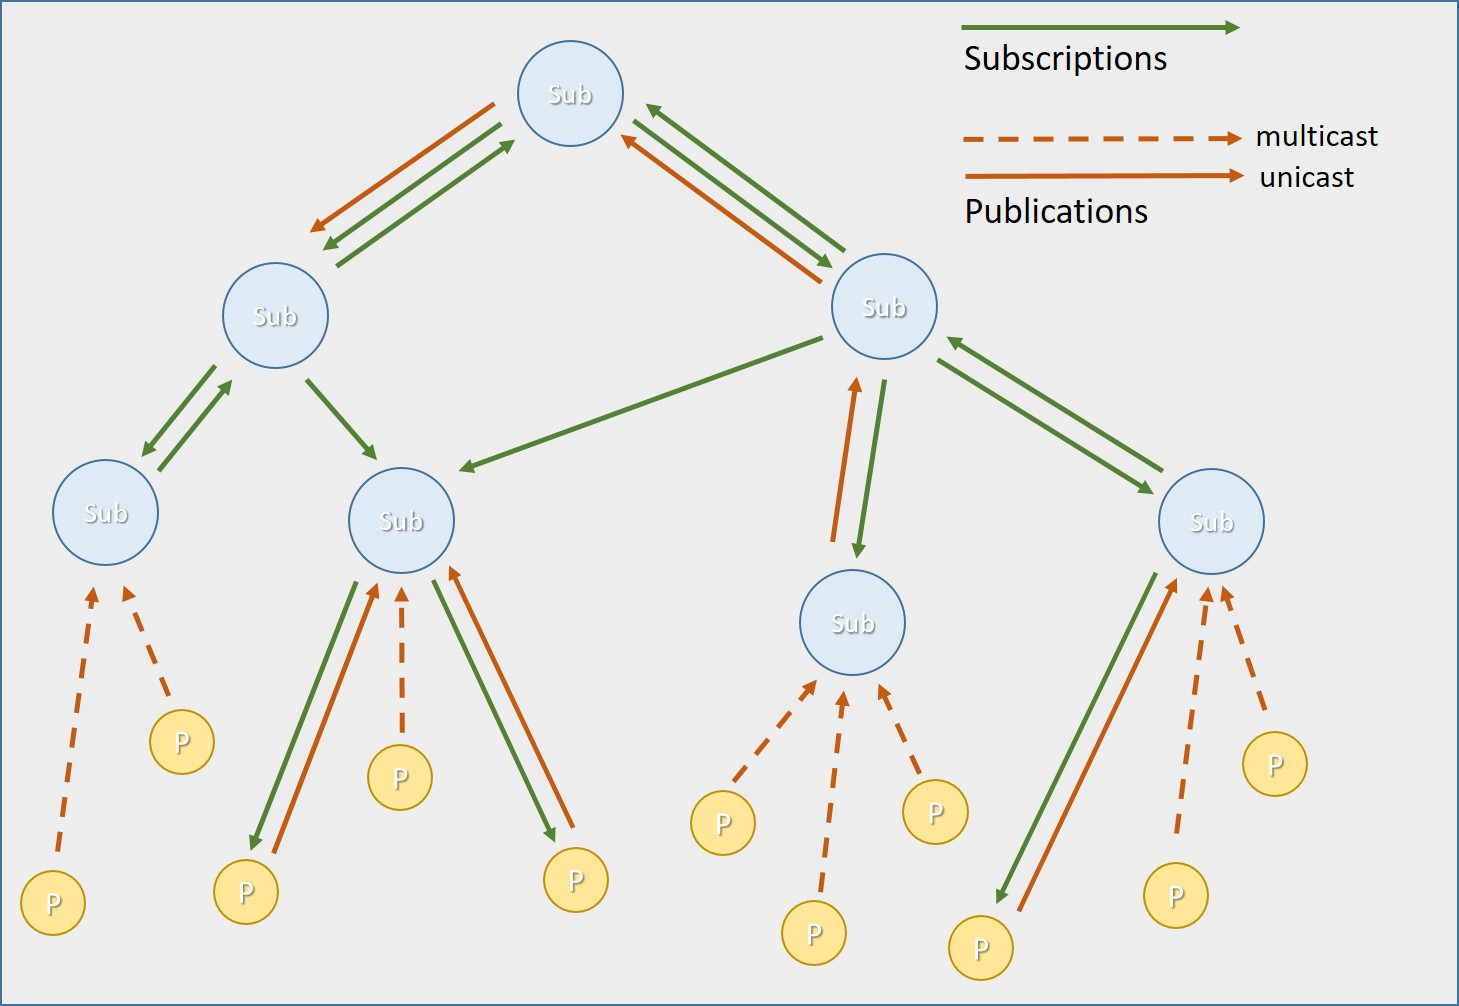
\includegraphics[width=\textwidth,height=\textheight/2,keepaspectratio=true]{dps_mesh.jpg}
\doxyfigcaption{D\+PS Mesh}
\end{DoxyImage}


Subscriptions flood throughout the network and can be forwarded in either direction, also there may be multiple routes. Publications only flow on routes that have matching subscriptions. Multicast publications are unsolicited and will be received by all nodes on the same subnet that are configured as multicast listeners. Unicast publications are only forwarded if the publication matches the subscriptions. In the steady state a publication reaching any node will be routed to all matching subscribers.\hypertarget{mesh-network_message-transports}{}\section{Transports}\label{mesh-network_message-transports}
\hypertarget{mesh-network_Multicast}{}\subsection{Multicast}\label{mesh-network_Multicast}
Multicast publications are wrapped in a Co\+AP envelope and sent to and received from the default Co\+AP port {\itshape 5683}.

A Co\+AP wrapped publication message is sent as a non-\/confirmable P\+UT request with options\+:
\begin{DoxyItemize}
\item Uri-\/\+Path\+: {\itshape dps/pub} 
\item Content-\/\+Format\+: {\itshape application/cbor} 
\end{DoxyItemize}

Control over sending and receiving multicast messages is provided via the {\itshape mcast\+Pub} parameter of \hyperlink{group__node_ga160d504bfaeb0d3711e0259000340fe3}{D\+P\+S\+\_\+\+Start\+Node()}.\hypertarget{mesh-network_Unicast}{}\subsection{Unicast}\label{mesh-network_Unicast}
D\+PS implements three different transports for sending and receiving unicast messages.

Unicast endpoints may be explicitly created and destroyed with \hyperlink{group__node_ga5064c63b8ce76bf34402e0c80183234b}{D\+P\+S\+\_\+\+Link()} and \hyperlink{group__node_ga79c86c3c0c5d6438b953a9acaab0ab0b}{D\+P\+S\+\_\+\+Unlink()}. The port used in unicast communication is provided via the {\itshape listen\+Port} parameter of \hyperlink{group__node_ga160d504bfaeb0d3711e0259000340fe3}{D\+P\+S\+\_\+\+Start\+Node()}.\hypertarget{mesh-network_UDP}{}\subsubsection{U\+DP}\label{mesh-network_UDP}
Each D\+PS message is contained in a single U\+DP datagram.\hypertarget{mesh-network_TCP}{}\subsubsection{T\+CP}\label{mesh-network_TCP}
Each D\+PS message is prefixed with the length of the message encoded as a C\+B\+OR unsigned integer value.\hypertarget{mesh-network_DTLS}{}\subsubsection{D\+T\+LS}\label{mesh-network_DTLS}
D\+T\+LS provides message authentication, integrity and confidentiality above U\+DP. Each D\+PS message is contained in a single D\+T\+LS datagram.

\begin{DoxySeeAlso}{See also}
\hyperlink{tutorials-security_enabling-network-layer-security}{Enabling network layer security} 
\end{DoxySeeAlso}

\chapter{Message Types and Flow}
\label{message-types-and-flow}
\Hypertarget{message-types-and-flow}
D\+PS has four message types\+: subscriptions, publications, acknowledgments, and subscription acknowledgements.

Subscriptions and publications are both inherently point-\/to-\/multipoint. An explicit assumption is that in IoT use cases there are many more publishers than subscribers. Publications are sent fairly frequently but subscriptions are relatively stable; subscriptions do not change frequently. To a large extent D\+PS has been designed around these assumptions. D\+PS would be good for implementing an IoT network with a large number of sensors but not ideal for implementing a highly scalable peer-\/to-\/peer chat service.

When a subscription does change only deltas for the subscription propagate through the network, this is typically less than a 100 bytes. Subscription acknowledgement messages are used to confirm that subscriptions are received at the next hop.

Publications are routed to all subscribers that have subscription topics that match the publication topics as described above.

Publications and acknowledgments can be accompanied by a payload, subscriptions do not carry a payload. Acknowledgements are optional and must be explicitly requested by the publisher when sending a publication. A subscriber can send an acknowledgement to the publisher along with an optional payload, the acknowledgement reaches the publisher by hop-\/by-\/hop forwarding in the reverse path of the publication. The reverse path ages out fairly quickly so acknowledgements should be sent as soon as possible after receipt of a publication. A publisher may receive multiple acknowledgments if there are multiple subscribers.\hypertarget{message-types-and-flow_message-encoding}{}\section{Encoding}\label{message-types-and-flow_message-encoding}
D\+PS messages are encoded in \href{https://tools.ietf.org/html/rfc7049}{\tt C\+B\+OR}, described below in \href{https://tools.ietf.org/html/draft-ietf-cbor-cddl-00}{\tt C\+D\+DL}.

Each message has the same form.

\begin{DoxyVerb}message = [
  version: 1,
  type: pub / sub / ack / sak,
  unprotected: { * field },
  protected: { * field },
  encrypted: { * field }
]
\end{DoxyVerb}
\hypertarget{message-types-and-flow_field-member-keys}{}\subsection{Field member keys}\label{message-types-and-flow_field-member-keys}
For compactness the member keys are encoded as integers as listed below.

\begin{DoxyVerb}field = (
  ? 1 => uint,               ; # port number sender is listening on
  ? 2 => int,                ; # ttl - time to live in seconds
  ? 3 => uuid,               ; # pub-id - unique identifier for a publication
  ? 4 => uint,               ; # seq-num - sequence number for a publication
  ? 5 => bool,               ; # ack-req - indicates if an publisher is requesting an acknowledgement
  ? 6 => bit-vector,         ; # bloom-filter -the bloom filter for a publication
  ? 7 => sub-flags,          ; # sub-flags - indicates delta or mute
  ? 8 => uuid,               ; # mesh-id - the mesh ID
  ? 9 => bit-vector,         ; # needs - the needs bit vector
  ? 10 => bit-vector,        ; # interests - the interests bit vector
  ? 11 => [ + topic: tstr ], ; # topics - the topic strings
  ? 12 => bstr               ; # data - payload data
)
\end{DoxyVerb}


The description of each message type includes what fields are mandatory or optional for each section.\hypertarget{message-types-and-flow_uuid}{}\subsection{U\+U\+ID}\label{message-types-and-flow_uuid}
U\+U\+I\+Ds identify publications and are also used as key identifiers for encrypted messages.

\begin{DoxyVerb}uuid = bstr .size 16
\end{DoxyVerb}
\hypertarget{message-types-and-flow_bit-vector-encoding}{}\subsection{Bit vector encoding}\label{message-types-and-flow_bit-vector-encoding}
The bit vector encoding includes control flags, the bit vector length expressed in bits and the raw or run-\/length encoded bit vector data.

\begin{DoxyVerb}bit-vector = [
  flags: uint .bits bit-vector-flags, ; # bit vector control flags
  len: uint,                          ; # bit vector length in bits
  bits: bstr                          ; # raw or rle-encoded bit vector
]
\end{DoxyVerb}
\hypertarget{message-types-and-flow_bit-vector-control-flags}{}\subsection{Bit vector control flags}\label{message-types-and-flow_bit-vector-control-flags}
Bits vectors are usually run-\/length encoded unless the raw unencoded bit vector is more compact than the rle-\/encoded representation. The rle-\/encoded flag indicates if the bit vector is encoded or raw.

The rle-\/complement flags indicates if the complement of the bit vector was was encoded. The bit vector complement is encoded if this results in a more compact encoding. This flag is only useful with run-\/length encoding.

\begin{DoxyVerb}bit-vector-flags = &(
  rle-encoded: 1,
  rle-complement: 2
)
\end{DoxyVerb}
\hypertarget{message-types-and-flow_subscription-flags}{}\subsection{Subscription flags}\label{message-types-and-flow_subscription-flags}
\begin{DoxyVerb}sub-flags = &(
  delta: 1,        ; # indicate interests is a delta
  mute: 2          ; # mute has been indicated
)
\end{DoxyVerb}
\hypertarget{message-types-and-flow_publication-message}{}\section{Publication message}\label{message-types-and-flow_publication-message}
\begin{DoxyVerb}pub = 1
\end{DoxyVerb}


{\itshape port} and {\itshape ttl} are mandatory in the {\itshape unprotected} section.

{\itshape ttl}, {\itshape pub-\/id}, {\itshape seq-\/num}, {\itshape ack-\/req} and {\itshape bloom-\/filter} are mandatory in the {\itshape protected} section.

{\itshape topics} and {\itshape data} are mandatory in the {\itshape encrypted} section.\hypertarget{message-types-and-flow_subscription-message}{}\section{Subscription message}\label{message-types-and-flow_subscription-message}
\begin{DoxyVerb}sub = 2
\end{DoxyVerb}


{\itshape port} and {\itshape seq-\/num} are mandatory in the {\itshape unprotected} section.

Additionally, in a regular subscription message, {\itshape sub-\/flags}, {\itshape mesh-\/id}, {\itshape needs} and {\itshape interests} are mandatory in the {\itshape unprotected} section. In an unlink subscription message those fields shall be absent.\hypertarget{message-types-and-flow_acknowledgement-message}{}\section{Acknowledgement message}\label{message-types-and-flow_acknowledgement-message}
\begin{DoxyVerb}ack = 3
\end{DoxyVerb}


{\itshape pub-\/id} and {\itshape seq-\/num} are mandatory in the {\itshape protected} section.

{\itshape data} is optional in the {\itshape encrypted} section.\hypertarget{message-types-and-flow_subscription-acknowledgement-message}{}\section{Subscription acknowledgement message}\label{message-types-and-flow_subscription-acknowledgement-message}
\begin{DoxyVerb}sak = 4
\end{DoxyVerb}


{\itshape port} and {\itshape seq-\/num} are mandatory in the {\itshape unprotected} section. 
\chapter{Data Series}
\label{data-series}
\Hypertarget{data-series}
D\+PS has built-\/in support for data series.

In addition to topic strings, every publication has a U\+U\+ID and serial number. Publications with same U\+U\+ID (and topic strings) form a series, the serial number is incremented each time the publication is sent to the network. The U\+U\+ID and serial number are available to the receiving subscribers. 
\chapter{Retained Publications}
\label{retained-publications}
\Hypertarget{retained-publications}
If there are no subscribers for the topic strings in a publication the publication will be discarded, typically at the first hop.

There are use cases where it is desirable for a publication to be held for later delivery. M\+Q\+TT has a feature that supports this use case; if an M\+Q\+TT publication is flagged as \char`\"{}retained\char`\"{} the M\+Q\+TT broker holds onto the publication until a subscriber is available to consume the message. D\+PS implements a similar feature where a T\+TL (time-\/to-\/live) can be set on a publication which is then held for delivery up until the time the T\+TL expires. For a publication to be retained it must match a subscription somewhere in the network, this allows specific nodes to take on responsibility for retaining matching publications. A retained publication can be replaced if the publisher sends a new publications having the same U\+U\+ID but a later serial number. A retained publication can be explicitly expired by sending a new publication with the same U\+U\+ID and a negative T\+TL.

Retained publications provide support for sleepy nodes, that is, nodes that are only periodically active on the network. For example, a wireless sensor node publishes a telemetry reading in the payload of a retained publication with a ten minute T\+TL then drops into low power mode waking within ten to deliver the next reading. The most recent telemetry will be available to subscribers no matter when they join the network. Similarly a sleepy subscriber can periodically connect to the network to receive publications updates. 
\chapter{Security}
\label{security}
\Hypertarget{security}
D\+PS has two security mechanisms\+: end-\/to-\/end encryption and link-\/layer encryption.

Publication and acknowledgement messages can be encrypted end-\/to-\/end. Messages are encrypted using \href{https://tools.ietf.org/html/rfc8152}{\tt C\+O\+SE}.

For privacy and to protect the network hop-\/by-\/hop links D\+PS uses link layer encryption where possible\+: D\+T\+LS for U\+DP, T\+LS for T\+CP, and transport-\/specific encryption for over non-\/\+IP networks. IP multicast packets do not use link-\/layer encryption. Because D\+PS is fundamentally a multi-\/hop mesh protocol payloads are secured end-\/to-\/end.

As noted above publications and acknowledgement messages can be encrypted using C\+O\+SE. The encryption in this case is end-\/to-\/end, the trust relationship is directly between the publishing node and the subscribing node, and intermediate nodes that simply route packets over the D\+PS mesh do not require a trust relationship with either the publishers or subscribers and do not hold decryption keys. The publication or acknowledgement data payload is encrypted, publications also carry the publication topic strings these are included in the encrypted payload. Message fields required for routing messages are integrity checked but obviously cannot be encrypted. The sending port number and T\+TL change on each hop so cannot be included in the end-\/to-\/end integrity check. The C\+O\+SE format includes an optional K\+ID (key-\/identifier) field. Encrypted D\+PS messages always have a K\+ID which allows the different publications to use different encryption keys.

Subscriptions do not carry payload data and the bit vectors carried in the payloads get recomputed at each hop. Unlike publications and acknowledgements, subscriptions do not use C\+O\+SE and rely solely on encryption at the link-\/layer.

Even when data is encrypted there are attack vectors based on traffic analysis. Traffic analysis is harder on a multi-\/hop mesh but because publications contain routing information that cannot be encrypted end-\/to-\/end. Specifically an attacker with access to a compromised node could use a dictionary attack to identify the topic strings in the publications and subscriptions flowing through that node. Where this is a concern the publishing and subscribing end-\/points can agree on a shared private encoding of topic strings, for example H\+M\+AC with a shared seed.

The following sections assume you are already familiar with the \hyperlink{message-types-and-flow_message-encoding}{message encoding }.\hypertarget{security_content-encryption}{}\section{Content Encryption}\label{security_content-encryption}
The {\itshape protected} section of a D\+PS message forms the protected attributes from the application as identified in C\+O\+SE. The {\itshape encrypted} section of a D\+PS message is the plaintext provided to the content encryption algorithm and is replaced by a C\+O\+SE object, either a {\itshape C\+O\+S\+E\+\_\+\+Encrypt\+\_\+\+Tagged} or {\itshape C\+O\+S\+E\+\_\+\+Encrypt0\+\_\+\+Tagged} object.

The implemented content encryption algorithms are {\itshape A\+E\+S-\/\+C\+C\+M-\/16-\/128-\/128} and {\itshape A\+E\+S-\/\+C\+C\+M-\/16-\/64-\/128}.\hypertarget{security_content-key-distribution}{}\section{Content Key Distribution}\label{security_content-key-distribution}
The encryption key is determined by the recipient algorithm. D\+PS supports the {\itshape direct}, {\itshape A128\+KW}, {\itshape E\+C\+D\+H-\/\+ES + H\+K\+D\+F-\/256}, and {\itshape E\+C\+D\+H-\/\+ES + A128\+KW} recipient algorithms.

The use of the key wrap variants allows multiple recipients to be included in a message.\hypertarget{security_elliptic-curve-keys}{}\subsection{Elliptic Curve Keys}\label{security_elliptic-curve-keys}
D\+PS supports the {\itshape N\+I\+ST P-\/256 (secp256r1)}, {\itshape N\+I\+ST P-\/384 (secp384r1)}, and {\itshape N\+I\+ST P-\/521 (secp521r1)} curves.

Point compression is not supported. Both the x and y coordinates must be included in EC key representations such as the ephemeral sender key.\hypertarget{security_key-derivation-functions}{}\subsection{Key Derivation Functions}\label{security_key-derivation-functions}
H\+K\+DF requires context information to be provided. This is represented in C\+O\+SE as the {\itshape C\+O\+S\+E\+\_\+\+K\+D\+F\+\_\+\+Context}.

The values of the {\itshape identity}, {\itshape nonce}, and {\itshape other} fields of the {\itshape Party\+U\+Info} and {\itshape Party\+V\+Info} structures in the {\itshape C\+O\+S\+E\+\_\+\+K\+D\+F\+\_\+\+Context} are {\itshape nil}.

{\itshape Supp\+Priv\+Info} is not included in the {\itshape C\+O\+S\+E\+\_\+\+K\+D\+F\+\_\+\+Context}.\hypertarget{security_counter-signatures}{}\section{Counter Signatures}\label{security_counter-signatures}
After encryption, the encrypted content is signed by the sender and the signature is included as a C\+O\+SE counter signature. This allows intermediate D\+PS nodes to authenticate the sender of a message without decrypting the contents of the message.

D\+PS supports the {\itshape E\+S256}, {\itshape E\+S384}, and {\itshape E\+S512} signature algorithms.\hypertarget{security_examples}{}\section{Examples}\label{security_examples}
An example encrypted publication message, using {\itshape A\+E\+S-\/\+C\+C\+M-\/16-\/128-\/128} for the content, {\itshape E\+C\+D\+H-\/\+E\+S+\+A128\+KW} for the key distribution, and {\itshape E\+S256} for signing, will look like\+:

\begin{DoxyVerb}message = [
  / version / 1,
  / type / 1,
  /unprotected / {
    / port / 1: 42446,
    / ttl / 2: 0
  },
  / protected (aad) / {
    / ttl / 2: 0,
    / pub-id / 3: h'17003AE54085EE56F735764C7631CE61',
    / seq-num / 4: 1,
    / ack-req / 5: false,
    / bloom-filter / 6: [1, 8192, h'002817805F00982A']
  },
  / encrypted (COSE_Encrypt_Tagged) / 96(
    [
      / protected / h'A101181E' / {
          \ alg \ 1: 30 \ AES-CCM-16-128-128 \
        } /,
      / unprotected / {
        / iv / 5: h'0100000017003AE54085EE56F7',
        / countersign / 7: [
          / protected / h'A10126' /
              \ alg \ 1: -7 \ ECDSA 256 \
            } /,
          / unprotected / {
            / kid / 4: h'4450532054657374205075626C6973686572'
          },
          / signature / h'1F14BDB559BB24A50B1C1ECA91938C445CFF64C4A24F075A6105B4679D19AEE439413AD30BE4C6C402031B2B04E7D6C2E4B2BA6A4C788E5C7DDE805654CA38CE'
        ]
      },
      / ciphertext / h'457C20BF6EB818AD98C4D820EFD2B017CACE97C47144E3D6',
      / recipients / [
        [
          / protected / h'A101381C' / {
              \ alg \ 1: -29 \ ECDH-ES+A128KW \
            } /,
          / unprotected / {
            / ephemeral / -1: {
              / kty / 1: 2,
              / crv / -1: 1,
              / x / -2: h'B34D696D855245BB79FCC8F0A328F37B7CC935803DAEC9EBAB97F061A68444E1',
              / y / -3: h'CDF27464CDC3A65DA7EC37139C354940E219A5E55D1A28265A015B2D0A47F72F'
            },
            / kid / 4: h'44505320546573742053756273637269626572'
          },
          / ciphertext / h'CF83EEA4B372FC210A374E44F040EEFA345C569C2D74A322'
        ]
      ]
    ]
  )
]
\end{DoxyVerb}
 
\chapter{Building and Running}
\label{building-and-running}
\Hypertarget{building-and-running}
\hypertarget{building-and-running_prerequisites}{}\section{Prerequisites}\label{building-and-running_prerequisites}
\hypertarget{building-and-running_prerequisites-linux}{}\subsection{Linux}\label{building-and-running_prerequisites-linux}

\begin{DoxyItemize}
\item gcc or clang
\item \href{http://scons.org/pages/download.html}{\tt S\+Cons}
\item libuv is used by node.\+js so packages are available for many distributions but note that D\+PS requires libuv 1.\+7 or later so it may be necessary to build libuv from source. \href{https://github.com/libuv}{\tt libuv source code on Git\+Hub.}
\item \href{http://www.swig.org/download.html}{\tt S\+W\+IG}
\end{DoxyItemize}\hypertarget{building-and-running_prerequisites-windows}{}\subsection{Windows}\label{building-and-running_prerequisites-windows}

\begin{DoxyItemize}
\item \href{https://www.visualstudio.com/downloads/}{\tt Visual Studio}

Note\+: In Visual Studio 2015, Visual C++ is not installed by default. When installing, be sure to choose {\bfseries Custom} installation and then choose the C++ components you require. Or, if Visual Studio is already installed, choose {\bfseries File $\vert$ New $\vert$ Project $\vert$ C++} and you will be prompted to install the necessary components.
\item \href{https://www.python.org/downloads/windows/}{\tt Latest Python 2.\+7 Release}
\item \href{http://scons.org/pages/download.html}{\tt S\+Cons}

Note\+: The S\+Cons installer will not detect the 64-\/bit installation of Python. Instead, download the zip file and follow the installation instructions in S\+Cons R\+E\+A\+D\+M\+E.\+txt.
\item \href{http://dist.libuv.org/dist/}{\tt libuv}
\item \href{http://www.swig.org/download.html}{\tt S\+W\+IG}
\end{DoxyItemize}\hypertarget{building-and-running_prerequisites-yocto}{}\subsection{Yocto}\label{building-and-running_prerequisites-yocto}
Yocto Project through the Open\+Embedded build system provides an open source development environment targeting the A\+RM, M\+I\+PS, Power\+PC and x86 architectures for a variety of platforms including x86-\/64 and emulated ones.


\begin{DoxyItemize}
\item \href{https://git.yoctoproject.org/}{\tt Yocto git}
\item \href{http://www.yoctoproject.org/docs/1.8/yocto-project-qs/yocto-project-qs.html}{\tt Yocto Project Quick Start}
\item \href{https://layers.openembedded.org/layerindex/recipe/32082/}{\tt Yocto libuv}
\end{DoxyItemize}\hypertarget{building-and-running_prerequisites-documentation}{}\subsection{Documentation}\label{building-and-running_prerequisites-documentation}
The C A\+PI documentation is generated using Doxygen. The Python (pydoc) and Java\+Script A\+PI (J\+S\+Doc) documentation is generated from the Doxygen output.

Doxygen can be downloaded from here\+: \href{http://www.stack.nl/~dimitri/doxygen/download.html}{\tt Doxygen}

Building the documentation requires the scons \href{https://bitbucket.org/scons/scons/wiki/DoxygenBuilder}{\tt Doxygen\+Builder} tool. This \href{https://bitbucket.org/scons/scons/wiki/ToolsIndex}{\tt page} has instructions on how to install the builder.\hypertarget{building-and-running_building}{}\section{Building}\label{building-and-running_building}
\hypertarget{building-and-running_building-linux-and-windows}{}\subsection{Linux and Windows}\label{building-and-running_building-linux-and-windows}
To build the D\+PS libraries, examples, bindings, and documentation run {\ttfamily scons}.

\begin{DoxyVerb}$ scons [variant=debug|release] [transport=udp|tcp|dtls] [bindings=all|none]
\end{DoxyVerb}


To build with a different compiler use the {\ttfamily CC} and {\ttfamily C\+XX} build options.

\begin{DoxyVerb}$ scons CC=clang CXX=clang++
\end{DoxyVerb}


To see the complete list of build options run {\ttfamily scons --help}. The default build configuration is {\ttfamily variant=release transport=udp bindings=all}.

\begin{DoxyNote}{Note}
A limitation of the current implementation is that the transport must be configured at compile time.
\end{DoxyNote}
The scons script pulls down source code from two external projects (mbedtls, and safestringlib) into the {\ttfamily ./ext} directory. If necessary these projects can be populated manually\+:

\begin{DoxyVerb}$ git clone https://github.com/ARMmbed/mbedtls ext/mbedtls
$ git clone https://github.com/01org/safestringlib.git ext/safestring
\end{DoxyVerb}


\begin{DoxyNote}{Note}
The ext projects are populated the first time D\+PS is built. To update these projects you need to manually do a {\ttfamily git pull} or delete the project directory and rerun scons.
\end{DoxyNote}
\hypertarget{building-and-running_building-yocto}{}\subsection{Yocto}\label{building-and-running_building-yocto}
Clone the poky repository and configure the Yocto environment. Refer to \href{http://www.yoctoproject.org/docs/1.8/yocto-project-qs/yocto-project-qs.html}{\tt Yocto Project Quick Start} for more information.

Clone the libuv Yocto project and yocto/recipes-\/connectivity/dps to the Yocto Project directory. Modify the value of S\+R\+C\+R\+E\+V\+\_\+dps in dps\+\_\+git.\+bb to the last commit of dps.

The Yocto Project directory needs to be included in B\+B\+L\+A\+Y\+E\+RS of conf/bblayers.\+conf. Refer to \href{https://wiki.yoctoproject.org/wiki/How_do_I}{\tt Yocto Wiki} for more information.

From the root directory of the Yocto Project, initialize the Yocto environment, provide a meaningful build directory name and build Yocto D\+PS.

\begin{DoxyVerb}$ source oe-init-build-env mybuilds
$ bitbake dps
\end{DoxyVerb}
\hypertarget{building-and-running_running}{}\section{Running}\label{building-and-running_running}
\hypertarget{building-and-running_running-examples}{}\subsection{Examples}\label{building-and-running_running-examples}
There are C, Python, and JS (node.\+js) examples.

The C examples are found in {\ttfamily ./examples}, the Python examples are in {\ttfamily ./py\+\_\+scripts} and the JS examples are in {\ttfamily ./js\+\_\+scripts}.

The C examples are installed in {\ttfamily ./build/dist/bin}. There are some some test scripts in {\ttfamily }./test\+\_\+scripts that run some more complex scenarios using the example programs. The test script {\ttfamily tree1} builds a small mesh and shows how publications sent to any node in the mesh get forwarded to the matching subscribers. The script {\ttfamily reg1} uses the {\ttfamily registry}, {\ttfamily reg\+\_\+pubs}, and {\ttfamily reg\+\_\+subs} examples programs to build a dynamic mesh using the experimental discovery service. 
\chapter{Tutorials}
\label{tutorials}
\Hypertarget{tutorials}
The tutorials provide an introduction into the D\+PS A\+P\+Is. It\textquotesingle{}s recommended they be read in the order below and assumes some familiarity with pub/sub terminology.

For compactness, the tutorials use the {\ttfamily a/b/c/d} topic string, where {\ttfamily a}, {\ttfamily b}, {\ttfamily c}, and {\ttfamily d} are the levels and {\ttfamily /} is the level separator, and strings for payload data. A real application would likely use more meaningful topic strings and structured payloads.


\begin{DoxyItemize}
\item \hyperlink{tutorials-hello-world}{Hello world}
\item \hyperlink{tutorials-link}{Building a D\+PS network}
\item \hyperlink{tutorials-security}{Securing the communications}
\end{DoxyItemize}

\begin{DoxySeeAlso}{See also}
\hyperlink{index}{Introduction}, \hyperlink{topic-strings}{Topic Strings}, \hyperlink{mesh-network}{Mesh Network}, \hyperlink{security}{Security} 
\end{DoxySeeAlso}
\hypertarget{tutorials-hello-world}{}\section{Hello world}\label{tutorials-hello-world}
\hypertarget{tutorials-hello-world_hello-world-prerequisites}{}\subsection{Prerequisites}\label{tutorials-hello-world_hello-world-prerequisites}

\begin{DoxyCodeInclude}
\textcolor{preprocessor}{#include <\hyperlink{dbg_8h}{dps/dbg.h}>}
\textcolor{preprocessor}{#include <\hyperlink{dps_8h}{dps/dps.h}>}
\end{DoxyCodeInclude}
 The first step in creating a D\+PS application is to include the necessary header files.\hypertarget{tutorials-hello-world_creating-a-node}{}\subsection{Creating a node}\label{tutorials-hello-world_creating-a-node}

\begin{DoxyCodeInclude}
    \textcolor{keyword}{const} \textcolor{keywordtype}{char} *separators = \textcolor{stringliteral}{"/."};
    \hyperlink{group__keystore_gaf3833cfe48f848f698514bc5daa075fa}{DPS\_KeyStore}* keyStore = NULL;
    \textcolor{keyword}{const} \hyperlink{struct___d_p_s___key_id}{DPS\_KeyId}* keyId = NULL;
    \hyperlink{group__node_ga4dd612ab965134321bb57fdb065f121c}{DPS\_Node}* node = \hyperlink{group__node_gaf6641b5bbf27b2c45ac7f926b0ce4efe}{DPS\_CreateNode}(separators, keyStore, keyId);
    \textcolor{keywordflow}{if} (!node) \{
        \textcolor{keywordflow}{goto} Exit;
    \}
\end{DoxyCodeInclude}
 Each entity in D\+PS is represented by a {\ttfamily D\+P\+S\+\_\+\+Node}. The node may be a publisher, subscriber, both, or neither. For this example, we\textquotesingle{}re going to be creating publisher and subscriber nodes.

Creating a node requires three parameters\+: the topic separators, a key store, and a key identifier. For now we\textquotesingle{}re only concerned with the separators. Key stores and identifiers are covered later when discussing how to secure communications.

The separators parameter is a string containing the characters used as topic level separators. Providing {\ttfamily /}. as the separators parameter value allows both {\ttfamily /} and {\ttfamily }. as separators.

\begin{DoxySeeAlso}{See also}
\hyperlink{group__node_gad19cf4272ba11e935654175c83db2ce1}{D\+P\+S\+\_\+\+Set\+Node\+Data()}, \hyperlink{group__node_ga65bba7bcfe5e940b153fcced4e2e8880}{D\+P\+S\+\_\+\+Get\+Node\+Data()}
\end{DoxySeeAlso}
\hypertarget{tutorials-hello-world_starting-a-node}{}\subsection{Starting a node}\label{tutorials-hello-world_starting-a-node}

\begin{DoxyCodeInclude}
    \textcolor{keywordtype}{int} mcastPub = \hyperlink{group__node_ga178a3a6450eeff450820fa34fd82049c}{DPS\_MCAST\_PUB\_ENABLE\_SEND} | 
      \hyperlink{group__node_gae493573fb2e02b87258952223eb4fcd7}{DPS\_MCAST\_PUB\_ENABLE\_RECV};
    uint16\_t listenPort = 0;
    \hyperlink{group__status_ga30395a84d3cad9d4ec29848106415038}{DPS\_Status} ret = \hyperlink{group__node_ga160d504bfaeb0d3711e0259000340fe3}{DPS\_StartNode}(node, mcastPub, listenPort);
    \textcolor{keywordflow}{if} (ret != \hyperlink{group__status_ga0ea3dd37bc558859ae0cb5a4f79a4bdd}{DPS\_OK}) \{
        \textcolor{keywordflow}{goto} Exit;
    \}
\end{DoxyCodeInclude}
 Once created, a node must be started. Starting a node enables it to begin sending and receiving D\+PS messages in the network.

For this example, we are going to be sending and receiving multicast publications so we enable both and let D\+PS assign the listening port.

\begin{DoxySeeAlso}{See also}
\hyperlink{group__node_gac939c83361ed89086f37c78d9c9009dd}{D\+P\+S\+\_\+\+M\+C\+A\+S\+T\+\_\+\+P\+U\+B\+\_\+\+D\+I\+S\+A\+B\+L\+ED}, \hyperlink{group__node_gaf920b28fe0721a7f97b11673494d7b36}{D\+P\+S\+\_\+\+Get\+Port\+Number()}
\end{DoxySeeAlso}
\hypertarget{tutorials-hello-world_publishing}{}\subsection{Publishing}\label{tutorials-hello-world_publishing}
\hypertarget{tutorials-hello-world_creating-a-publication}{}\subsubsection{Creating a publication}\label{tutorials-hello-world_creating-a-publication}

\begin{DoxyCodeInclude}
    \hyperlink{group__publication_ga0d439693474aa54e27f3d45a054696ac}{DPS\_Publication}* pub = \hyperlink{group__publication_gaca070a96a6374e99a05d647c10737962}{DPS\_CreatePublication}(node);
    \textcolor{keywordflow}{if} (!pub) \{
        \textcolor{keywordflow}{goto} Exit;
    \}
    \textcolor{keyword}{const} \textcolor{keywordtype}{char}* topics[] = \{
        \textcolor{stringliteral}{"a/b/c/d"}
    \};
    \textcolor{keywordtype}{size\_t} numTopics = A\_SIZEOF(topics);
    \textcolor{keywordtype}{int} noWildCard = \hyperlink{dps_8h_ad8b397975a479b996ef223367d8835a9}{DPS\_FALSE};
    ret = \hyperlink{group__publication_ga7b0709e28cb34d5a30b90e4142cd6c19}{DPS\_InitPublication}(pub, topics, numTopics, noWildCard, NULL, NULL);
    \textcolor{keywordflow}{if} (ret != \hyperlink{group__status_ga0ea3dd37bc558859ae0cb5a4f79a4bdd}{DPS\_OK}) \{
        \textcolor{keywordflow}{goto} Exit;
    \}
\end{DoxyCodeInclude}
 Each publication in D\+PS is represented by a {\ttfamily D\+P\+S\+\_\+\+Publication}. Each publication has a set of topics, a U\+U\+ID, and a sequence number. In this example we are creating a publication with one topic, {\ttfamily a/b/c/d}. The U\+U\+ID is assigned by D\+PS and the sequence number will be incremented each time we publish.

The {\ttfamily no\+Wild\+Card} parameter is used by the publisher to control whether a subscription is required to match the publication\textquotesingle{}s topics exactly or can use wildcards to match the topics. If we set {\ttfamily no\+Wild\+Card} to {\ttfamily D\+P\+S\+\_\+\+T\+R\+UE} then only a subscription to {\ttfamily a/b/c/d} will receive this publication. This allows the publisher to prevent publications being sent to catchall subscriptions such as {\ttfamily +/\#}. Since we set {\ttfamily no\+Wild\+Card} to {\ttfamily D\+P\+S\+\_\+\+F\+A\+L\+SE} here, subscriptions to {\ttfamily a/\#}, {\ttfamily a/+/+/d}, or similar variations will receive this publication.

Both the publication\textquotesingle{}s key identifier and acknowledgement handler are set to {\ttfamily N\+U\+LL} here; they are covered in later sections.

\begin{DoxySeeAlso}{See also}
\hyperlink{group__publication_ga91c46ccb6df7f4bb99ca5d9d35cc5a4a}{D\+P\+S\+\_\+\+Set\+Publication\+Data()}, \hyperlink{group__publication_gaa8bee35089ac62289c9ba0e6a0568ca0}{D\+P\+S\+\_\+\+Get\+Publication\+Data()}, \hyperlink{group__publication_gad2a37d52f12c93434b431eefd732f363}{D\+P\+S\+\_\+\+Publication\+Get\+Node()}, \hyperlink{group__publication_gaba1ad3ee807b75a1281d334be06a12f7}{D\+P\+S\+\_\+\+Publication\+Get\+U\+U\+I\+D()}, \hyperlink{group__publication_ga875b48217d861d4a9fa5471419d354e9}{D\+P\+S\+\_\+\+Publication\+Get\+Sequence\+Num()}
\end{DoxySeeAlso}
\hypertarget{tutorials-hello-world_sending-a-publication}{}\subsubsection{Sending a publication}\label{tutorials-hello-world_sending-a-publication}

\begin{DoxyCodeInclude}
    \textcolor{keyword}{const} \textcolor{keywordtype}{char}* payload = \textcolor{stringliteral}{"Hello"};
    \textcolor{keywordtype}{size\_t} numPayloadBytes = strlen(payload) + 1;
    int16\_t ttl = 0;
    ret = \hyperlink{group__publication_ga828a4efc5c235c48a81f6460cc3fe416}{DPS\_Publish}(pub, (\textcolor{keyword}{const} uint8\_t*)payload, numPayloadBytes, ttl);
    \textcolor{keywordflow}{if} (ret != \hyperlink{group__status_ga0ea3dd37bc558859ae0cb5a4f79a4bdd}{DPS\_OK}) \{
        \textcolor{keywordflow}{goto} Exit;
    \}
\end{DoxyCodeInclude}
 Once created and initialized with a set of topics, application payloads may be sent. Payload data is simply an array of bytes in D\+PS, no assumptions are made with regards to the payload format.

In this example the {\ttfamily ttl} parameter is zero, indicating that the publication will be sent best-\/effort to all active subscribing nodes. A non-\/zero ttl is referred to as a retained publication and is covered later.

A publisher may send additional publications via the same {\ttfamily D\+P\+S\+\_\+\+Publication}. Each additional send increments the sequence number of the publication.\hypertarget{tutorials-hello-world_subscribing}{}\subsection{Subscribing}\label{tutorials-hello-world_subscribing}
\hypertarget{tutorials-hello-world_creating-a-subscription}{}\subsubsection{Creating a subscription}\label{tutorials-hello-world_creating-a-subscription}

\begin{DoxyCodeInclude}
    \textcolor{keyword}{const} \textcolor{keywordtype}{char}* topics[] = \{
        \textcolor{stringliteral}{"a/b/c/d"}
    \};
    \textcolor{keywordtype}{size\_t} numTopics = A\_SIZEOF(topics);
    \hyperlink{group__subscription_gadb927c4c1b7306867a75fc4288b54af7}{DPS\_Subscription}* sub = \hyperlink{group__subscription_ga4095bb00bd0ca7fa9614ebbc2c28199f}{DPS\_CreateSubscription}(node, topics, 
      numTopics);
    \textcolor{keywordflow}{if} (!sub) \{
        \textcolor{keywordflow}{goto} Exit;
    \}
\end{DoxyCodeInclude}
 Each subscription in D\+PS is represented by a {\ttfamily D\+P\+S\+\_\+\+Subscription}. In this example we are creating a subscription with one topic with no wildcards, {\ttfamily a/b/c/d}.

Wildcards may be used to match a broader set of topics. A {\ttfamily +} matches any single topic level, and a {\ttfamily \#} matches all topic levels from that level on. In this instance since the publisher is allowing wildcard matching, the subscriber could use either {\ttfamily a/b/+/d} or {\ttfamily a/\#} (among others) as the topic and still receive the publication.

A subscription may also be created with multiple topics. The publication must include {\itshape all} of the topics to be received.

\begin{DoxySeeAlso}{See also}
\hyperlink{group__subscription_gad581d341003e20c714061e44b57c2009}{D\+P\+S\+\_\+\+Set\+Subscription\+Data()}, \hyperlink{group__subscription_ga88ab2284734f099ef67bcc60997142b3}{D\+P\+S\+\_\+\+Get\+Subscription\+Data()}, \hyperlink{group__subscription_gafea65751c811555736c8c65fcb3a9480}{D\+P\+S\+\_\+\+Subscription\+Get\+Node()}
\end{DoxySeeAlso}
\hypertarget{tutorials-hello-world_receiving-a-publication}{}\subsubsection{Receiving a publication}\label{tutorials-hello-world_receiving-a-publication}

\begin{DoxyCodeInclude}
        ret = \hyperlink{group__subscription_ga83234ea82a91e07e3f5894a4dcf5267e}{DPS\_Subscribe}(sub, PublicationHandler);
        \textcolor{keywordflow}{if} (ret != \hyperlink{group__status_ga0ea3dd37bc558859ae0cb5a4f79a4bdd}{DPS\_OK}) \{
            \textcolor{keywordflow}{goto} Exit;
        \}
\end{DoxyCodeInclude}
 Publications are received asynchronously. The first step in receiving a publication is to provide the publication handler to D\+PS and start the subscription. The publication handler will be called for each received publication.

\begin{DoxyNote}{Note}
Each instance of {\ttfamily D\+P\+S\+\_\+\+Node} creates and runs its own thread. The lifetime of this thread is the same as the lifetime of the node. The publication handler is dispatched from this thread.
\end{DoxyNote}

\begin{DoxyCodeInclude}
\textcolor{keyword}{static} \textcolor{keywordtype}{void} PublicationHandler(\hyperlink{group__subscription_gadb927c4c1b7306867a75fc4288b54af7}{DPS\_Subscription}* sub, \textcolor{keyword}{const} 
      \hyperlink{group__publication_ga0d439693474aa54e27f3d45a054696ac}{DPS\_Publication}* pub,
                               uint8\_t* payload, \textcolor{keywordtype}{size\_t} numPayloadBytes)
\{
    \textcolor{keywordtype}{size\_t} i;

    \textcolor{keywordflow}{for} (i = 0; i < \hyperlink{group__subscription_gab0ad2c6806f8f44f27c70fff915b7e9a}{DPS\_SubscriptionGetNumTopics}(sub); ++i) \{
        \textcolor{keyword}{const} \textcolor{keywordtype}{char}* topic = \hyperlink{group__subscription_gaacc63deda2f2d97cf3f44ca84784b2f6}{DPS\_SubscriptionGetTopic}(sub, i);
        \hyperlink{group__debug_gaf1d25cc7f1d2d92f96ba620217af28fd}{DPS\_PRINT}(\textcolor{stringliteral}{"subscription topic[%ld]=%s\(\backslash\)n"}, i, topic);
    \}

    \textcolor{keyword}{const} \hyperlink{struct___d_p_s___u_u_i_d}{DPS\_UUID}* uuid = \hyperlink{group__publication_gaba1ad3ee807b75a1281d334be06a12f7}{DPS\_PublicationGetUUID}(pub);
    \hyperlink{group__debug_gaf1d25cc7f1d2d92f96ba620217af28fd}{DPS\_PRINT}(\textcolor{stringliteral}{"uuid=%s\(\backslash\)n"}, \hyperlink{group__uuid_ga9c51faa57ecb228ce7eda077a90b20ff}{DPS\_UUIDToString}(uuid));

    uint32\_t n = \hyperlink{group__publication_ga875b48217d861d4a9fa5471419d354e9}{DPS\_PublicationGetSequenceNum}(pub);
    \hyperlink{group__debug_gaf1d25cc7f1d2d92f96ba620217af28fd}{DPS\_PRINT}(\textcolor{stringliteral}{"sequence number=%d\(\backslash\)n"}, n);

    \textcolor{keywordflow}{for} (i = 0; i < \hyperlink{group__publication_gaee6fc3b13484faacff0d26646778f777}{DPS\_PublicationGetNumTopics}(pub); ++i) \{
        \textcolor{keyword}{const} \textcolor{keywordtype}{char}* topic = \hyperlink{group__publication_ga143a5c6fbe0bdf1725e841f122582432}{DPS\_PublicationGetTopic}(pub, i);
        \hyperlink{group__debug_gaf1d25cc7f1d2d92f96ba620217af28fd}{DPS\_PRINT}(\textcolor{stringliteral}{"publication topic[%ld]=%s\(\backslash\)n"}, i, topic);
    \}

    \hyperlink{group__debug_gaf1d25cc7f1d2d92f96ba620217af28fd}{DPS\_PRINT}(\textcolor{stringliteral}{"payload=%.*s\(\backslash\)n"}, numPayloadBytes, payload);
\}
\end{DoxyCodeInclude}
 This publication handler exercises the A\+P\+Is for retrieving the subscription and publication information.\hypertarget{tutorials-hello-world_acknowledging}{}\subsection{Acknowledging}\label{tutorials-hello-world_acknowledging}
Acknowledgements provide an optional means for subscribers to reply to publications. For example, they may be used when the publication is logically a request and the acknowledgements are responses. Similar to publications, acknowledgements may include an application payload, and no assumptions are made by D\+PS with regards to the acknowledgement payload format.\hypertarget{tutorials-hello-world_requesting-an-acknowledgement}{}\subsubsection{Requesting an acknowledgement}\label{tutorials-hello-world_requesting-an-acknowledgement}

\begin{DoxyCodeInclude}
    \hyperlink{group__publication_ga0d439693474aa54e27f3d45a054696ac}{DPS\_Publication}* pub = \hyperlink{group__publication_gaca070a96a6374e99a05d647c10737962}{DPS\_CreatePublication}(node);
    \textcolor{keywordflow}{if} (!pub) \{
        \textcolor{keywordflow}{goto} Exit;
    \}
    \textcolor{keyword}{const} \textcolor{keywordtype}{char}* topics[] = \{
        \textcolor{stringliteral}{"a/b/c/d"}
    \};
    \textcolor{keywordtype}{size\_t} numTopics = A\_SIZEOF(topics);
    \textcolor{keywordtype}{int} noWildCard = \hyperlink{dps_8h_ad8b397975a479b996ef223367d8835a9}{DPS\_FALSE};
    ret = \hyperlink{group__publication_ga7b0709e28cb34d5a30b90e4142cd6c19}{DPS\_InitPublication}(pub, topics, numTopics, noWildCard, NULL,
                              AcknowledgementHandler);
    \textcolor{keywordflow}{if} (ret != \hyperlink{group__status_ga0ea3dd37bc558859ae0cb5a4f79a4bdd}{DPS\_OK}) \{
        \textcolor{keywordflow}{goto} Exit;
    \}
\end{DoxyCodeInclude}
 Requesting an acknowledgement is identical to \hyperlink{tutorials-hello-world_creating-a-publication}{Creating a publication}, with the addition of the {\ttfamily D\+P\+S\+\_\+\+Acknowledgement\+Handler}.\hypertarget{tutorials-hello-world_sending-an-acknowledgement}{}\subsubsection{Sending an acknowledgement}\label{tutorials-hello-world_sending-an-acknowledgement}

\begin{DoxyCodeInclude}
    \textcolor{keywordflow}{if} (\hyperlink{group__publication_ga516f7f314c7b95210751d00285758b9b}{DPS\_PublicationIsAckRequested}(pub)) \{
        \textcolor{keyword}{const} \textcolor{keywordtype}{char}* payload = \textcolor{stringliteral}{"World"};
        \textcolor{keywordtype}{size\_t} numPayloadBytes = strlen(payload) + 1;
        \hyperlink{group__status_ga30395a84d3cad9d4ec29848106415038}{DPS\_Status} ret = \hyperlink{group__publication_ga308074429a566ffb8d04d55bae520b04}{DPS\_AckPublication}(pub, (\textcolor{keyword}{const} uint8\_t*)payload, 
      numPayloadBytes);
        \textcolor{keywordflow}{if} (ret != \hyperlink{group__status_ga0ea3dd37bc558859ae0cb5a4f79a4bdd}{DPS\_OK}) \{
            \textcolor{keywordflow}{goto} Exit;
        \}
    \}
\end{DoxyCodeInclude}
 To determine if a publication has requested an ack, call \hyperlink{group__publication_ga516f7f314c7b95210751d00285758b9b}{D\+P\+S\+\_\+\+Publication\+Is\+Ack\+Requested()}. To send an acknowledgement, along with any optional acknowledgement payload, call \hyperlink{group__publication_ga308074429a566ffb8d04d55bae520b04}{D\+P\+S\+\_\+\+Ack\+Publication()}.

The {\ttfamily pub} parameter of the publication handler is only valid during the body of the handler. In order to acknowledge a publication after the handler has returned, the application must first call \hyperlink{group__publication_ga41f31a8b63558e13d73d96de6086e5c4}{D\+P\+S\+\_\+\+Copy\+Publication()} to create a partial copy of the publication. The copy may be used after the handler returns.\hypertarget{tutorials-hello-world_receiving-an-acknowledgement}{}\subsubsection{Receiving an acknowledgement}\label{tutorials-hello-world_receiving-an-acknowledgement}

\begin{DoxyCodeInclude}
\textcolor{keyword}{static} \textcolor{keywordtype}{void} AcknowledgementHandler(\hyperlink{group__publication_ga0d439693474aa54e27f3d45a054696ac}{DPS\_Publication}* pub,
                                   uint8\_t* payload, \textcolor{keywordtype}{size\_t} numPayloadBytes)
\{
    \textcolor{keywordtype}{size\_t} i;

    \textcolor{keyword}{const} \hyperlink{struct___d_p_s___u_u_i_d}{DPS\_UUID}* uuid = \hyperlink{group__publication_gaba1ad3ee807b75a1281d334be06a12f7}{DPS\_PublicationGetUUID}(pub);
    \hyperlink{group__debug_gaf1d25cc7f1d2d92f96ba620217af28fd}{DPS\_PRINT}(\textcolor{stringliteral}{"uuid=%s\(\backslash\)n"}, \hyperlink{group__uuid_ga9c51faa57ecb228ce7eda077a90b20ff}{DPS\_UUIDToString}(uuid));

    uint32\_t n = \hyperlink{group__publication_ga875b48217d861d4a9fa5471419d354e9}{DPS\_PublicationGetSequenceNum}(pub);
    \hyperlink{group__debug_gaf1d25cc7f1d2d92f96ba620217af28fd}{DPS\_PRINT}(\textcolor{stringliteral}{"sequence number=%d\(\backslash\)n"}, n);

    \textcolor{keywordflow}{for} (i = 0; i < \hyperlink{group__publication_gaee6fc3b13484faacff0d26646778f777}{DPS\_PublicationGetNumTopics}(pub); ++i) \{
        \textcolor{keyword}{const} \textcolor{keywordtype}{char}* topic = \hyperlink{group__publication_ga143a5c6fbe0bdf1725e841f122582432}{DPS\_PublicationGetTopic}(pub, i);
        \hyperlink{group__debug_gaf1d25cc7f1d2d92f96ba620217af28fd}{DPS\_PRINT}(\textcolor{stringliteral}{"publication topic[%ld]=%s\(\backslash\)n"}, i, topic);
    \}

    \hyperlink{group__debug_gaf1d25cc7f1d2d92f96ba620217af28fd}{DPS\_PRINT}(\textcolor{stringliteral}{"payload=%.*s\(\backslash\)n"}, numPayloadBytes, payload);
\}
\end{DoxyCodeInclude}
 Acknowledgements are received asynchronously. The acknowledgement handler will be called for each received acknowledgement.

This acknowledgement handler exercises the A\+P\+Is for retrieving the publication information associated with the acknowledgement.

\begin{DoxyNote}{Note}
The acknowledgement handler is dispatched from the {\ttfamily D\+P\+S\+\_\+\+Node\textquotesingle{}s} thread. 
\end{DoxyNote}
\hypertarget{tutorials-link}{}\section{Building a D\+PS network}\label{tutorials-link}
The \hyperlink{tutorials-hello-world}{Hello world} tutorial showed how to build a simple multicast publisher and subscriber network. This tutorial will show how to use the link functionality of D\+PS to create more complex networks that can span subnets.

As before, we need to create nodes for the publisher and subscriber using \hyperlink{tutorials-hello-world_creating-a-node}{D\+P\+S\+\_\+\+Create\+Node() }. But this time we will create a third type of node that is neither a publisher or subscriber that will forward publications and subscriptions between the publisher and subscriber nodes.\hypertarget{tutorials-link_starting-a-unicast-node}{}\subsection{Starting a node}\label{tutorials-link_starting-a-unicast-node}

\begin{DoxyCodeInclude}
    \textcolor{keywordtype}{int} mcastPub = \hyperlink{group__node_gac939c83361ed89086f37c78d9c9009dd}{DPS\_MCAST\_PUB\_DISABLED};
    uint16\_t listenPort = port;
    \hyperlink{group__status_ga30395a84d3cad9d4ec29848106415038}{DPS\_Status} ret = \hyperlink{group__node_ga160d504bfaeb0d3711e0259000340fe3}{DPS\_StartNode}(node, mcastPub, listenPort);
    \textcolor{keywordflow}{if} (ret != \hyperlink{group__status_ga0ea3dd37bc558859ae0cb5a4f79a4bdd}{DPS\_OK}) \{
        \textcolor{keywordflow}{goto} Exit;
    \}
    uint16\_t portNum = \hyperlink{group__node_gaf920b28fe0721a7f97b11673494d7b36}{DPS\_GetPortNumber}(node);
\end{DoxyCodeInclude}
 The first thing we will do is disable multicast sending and receiving for our three nodes by using \hyperlink{group__node_gac939c83361ed89086f37c78d9c9009dd}{D\+P\+S\+\_\+\+M\+C\+A\+S\+T\+\_\+\+P\+U\+B\+\_\+\+D\+I\+S\+A\+B\+L\+ED} for the {\ttfamily mcast\+Pub} parameter of \hyperlink{group__node_ga160d504bfaeb0d3711e0259000340fe3}{D\+P\+S\+\_\+\+Start\+Node()}. All publications and subscriptions will go through the forwarding node.

The second thing we do is specify the {\ttfamily listen\+Port} parameter to \hyperlink{group__node_ga160d504bfaeb0d3711e0259000340fe3}{D\+P\+S\+\_\+\+Start\+Node()}. A value of zero lets D\+PS assign an ephemeral listening port. A value of non-\/zero requests a specific port.

The last thing we do is get the ephemeral port D\+PS has chosen with \hyperlink{group__node_gaf920b28fe0721a7f97b11673494d7b36}{D\+P\+S\+\_\+\+Get\+Port\+Number()}. This will be used by the subscriber and publisher to link to the forwarding node.\hypertarget{tutorials-link_linking}{}\subsection{Linking to a node}\label{tutorials-link_linking}

\begin{DoxyCodeInclude}
        \hyperlink{group__nodeaddress_ga9e9f56aa38e82b4edcef7eb81e9f5bd2}{DPS\_NodeAddress}* addr = \hyperlink{group__nodeaddress_ga6bed18a4b0ad533ec88c7a0d376de818}{DPS\_CreateAddress}();
        \textcolor{keywordflow}{if} (!addr) \{
            \textcolor{keywordflow}{goto} Exit;
        \}

        \textcolor{keyword}{struct }sockaddr\_in saddr;
        memset(&saddr, 0, \textcolor{keyword}{sizeof}(saddr));
        saddr.sin\_family = AF\_INET;
        saddr.sin\_port = htons(linkPort);
        saddr.sin\_addr.s\_addr = htonl(INADDR\_LOOPBACK);

        \hyperlink{group__nodeaddress_ga6231c243c483bd2d282f7df734a98946}{DPS\_SetAddress}(addr, (\textcolor{keyword}{const} \textcolor{keyword}{struct} sockaddr*)&saddr);

        ret = \hyperlink{group__node_ga5064c63b8ce76bf34402e0c80183234b}{DPS\_Link}(node, addr, LinkComplete, NULL);
        \hyperlink{group__nodeaddress_ga1f373831e8009ff5959ccb02b8c3fb14}{DPS\_DestroyAddress}(addr);
        \textcolor{keywordflow}{if} (ret != \hyperlink{group__status_ga0ea3dd37bc558859ae0cb5a4f79a4bdd}{DPS\_OK}) \{
            \textcolor{keywordflow}{goto} Exit;
        \}
\end{DoxyCodeInclude}
 Now that we know the host ({\ttfamily localhost} in this example) and listening port of the forwarding node, we can call \hyperlink{group__node_ga5064c63b8ce76bf34402e0c80183234b}{D\+P\+S\+\_\+\+Link()} to create the link from the subscriber and publisher to the forwarding node. In order to do this we must first create a \hyperlink{group__nodeaddress_ga9e9f56aa38e82b4edcef7eb81e9f5bd2}{D\+P\+S\+\_\+\+Node\+Address} and set its value to the host and port of the forwarding node.

Once we call \hyperlink{group__node_ga5064c63b8ce76bf34402e0c80183234b}{D\+P\+S\+\_\+\+Link()} we can destroy the \hyperlink{group__nodeaddress_ga9e9f56aa38e82b4edcef7eb81e9f5bd2}{D\+P\+S\+\_\+\+Node\+Address} as we don\textquotesingle{}t need it anymore while we wait for the asynchronous link to complete.


\begin{DoxyCodeInclude}
\textcolor{keyword}{static} \textcolor{keywordtype}{void} LinkComplete(\hyperlink{group__node_ga4dd612ab965134321bb57fdb065f121c}{DPS\_Node}* node, \hyperlink{group__nodeaddress_ga9e9f56aa38e82b4edcef7eb81e9f5bd2}{DPS\_NodeAddress}* addr, 
      \hyperlink{group__status_ga30395a84d3cad9d4ec29848106415038}{DPS\_Status} status, \textcolor{keywordtype}{void}* data)
\{
    \hyperlink{group__debug_gaf1d25cc7f1d2d92f96ba620217af28fd}{DPS\_PRINT}(\textcolor{stringliteral}{"Linked to %s\(\backslash\)n"}, \hyperlink{group__nodeaddress_gafc7b21048f92370ca29325d6245b576d}{DPS\_NodeAddrToString}(addr));
\}
\end{DoxyCodeInclude}
 The link is now complete and we can proceed with \hyperlink{tutorials-hello-world_receiving-a-publication}{subscribing } or \hyperlink{tutorials-hello-world_sending-a-publication}{publishing } as before.

\begin{DoxyNote}{Note}
The link complete callback is dispatched from the {\ttfamily D\+P\+S\+\_\+\+Node\textquotesingle{}s} thread.
\end{DoxyNote}
\begin{DoxySeeAlso}{See also}
\hyperlink{group__node_ga79c86c3c0c5d6438b953a9acaab0ab0b}{D\+P\+S\+\_\+\+Unlink()}, \hyperlink{group__node_ga0bd13b2bd395bbc7807ecc899a8862f1}{D\+P\+S\+\_\+\+Link\+To()}, \hyperlink{group__node_ga2d5bb0528c2a171991ad6355cbadac69}{D\+P\+S\+\_\+\+Unlink\+From()} 
\end{DoxySeeAlso}
\hypertarget{tutorials-security}{}\section{Securing the communications}\label{tutorials-security}
\hypertarget{tutorials-security_enabling-network-layer-security}{}\subsection{Enabling network layer security}\label{tutorials-security_enabling-network-layer-security}
Network layer security can be used to secure unicast communications between two nodes (a single hop). This includes the subscription, acknowledgement, and subscription acknowledgement messages. When the two nodes are \hyperlink{tutorials-link}{linked }, it also includes publications. Multicast publications are not secured. One of the end-\/to-\/end mechanisms described below must be used to secure multicast publications.

The first step to enabling network layer security is to build with a transport that supports it.


\begin{DoxyCode}
$ scons transport=dtls
\end{DoxyCode}


The D\+T\+LS transport supports two mechanisms for securing the connection\+: pre-\/shared keys, and certificates.\hypertarget{tutorials-security_dtls-with-pre-shared-keys}{}\subsubsection{D\+T\+L\+S with pre-\/shared keys}\label{tutorials-security_dtls-with-pre-shared-keys}

\begin{DoxyCodeInclude}
\textcolor{preprocessor}{#define BYTE\_STR(s) \{ (const uint8\_t*)s, sizeof(s) - 1 \}}
\textcolor{keyword}{static} \textcolor{keyword}{const} \hyperlink{struct___d_p_s___key}{DPS\_Key} PSK = \{ \hyperlink{group__keystore_gga7ca1045749c725e9c4a1b4758b2a0196a662c1e84628d96be8ae08163af382392}{DPS\_KEY\_SYMMETRIC}, \{ .symmetric = BYTE\_STR(\textcolor{stringliteral}{"1234"}) \} \}
      ;
\textcolor{keyword}{static} \textcolor{keyword}{const} \hyperlink{struct___d_p_s___key_id}{DPS\_KeyId} PSK\_ID = BYTE\_STR(\textcolor{stringliteral}{"Tutorial Network PSK"});
\end{DoxyCodeInclude}
To use pre-\/shared keys (P\+S\+Ks), we\textquotesingle{}ll need to agree on a P\+SK and its identifier. {\ttfamily B\+Y\+T\+E\+\_\+\+S\+TR} is a convenience macro used in the tutorials for using strings anywhere a buffer and its length is expected in the A\+P\+Is.


\begin{DoxyCodeInclude}
    \textcolor{keyword}{const} \textcolor{keywordtype}{char} *separators = \textcolor{stringliteral}{"/."};
    \hyperlink{group__keystore_gaf3833cfe48f848f698514bc5daa075fa}{DPS\_KeyStore}* keyStore = \hyperlink{group__keystore_gafa79de23848ff56d0cced67897313369}{DPS\_CreateKeyStore}(PskAndIdHandler, PskHandler, 
      NULL, NULL);
    \textcolor{keyword}{const} \hyperlink{struct___d_p_s___key_id}{DPS\_KeyId}* keyId = NULL;
    \hyperlink{group__node_ga4dd612ab965134321bb57fdb065f121c}{DPS\_Node}* node = \hyperlink{group__node_gaf6641b5bbf27b2c45ac7f926b0ce4efe}{DPS\_CreateNode}(separators, keyStore, keyId);
    \textcolor{keywordflow}{if} (!node) \{
        \textcolor{keywordflow}{goto} Exit;
    \}
\end{DoxyCodeInclude}
All of the security mechanisms require that the node be created with a key store. The D\+T\+LS P\+SK mechanism requires that a \hyperlink{group__keystore_ga83d3ade4f4acd7d4385d606270ddfd29}{D\+P\+S\+\_\+\+Key\+And\+Id\+Handler} and \hyperlink{group__keystore_gaccf7e3d43bc1e586132d7f1ae03d02f7}{D\+P\+S\+\_\+\+Key\+Handler} be provided.


\begin{DoxyCodeInclude}
\textcolor{keyword}{static} \hyperlink{group__status_ga30395a84d3cad9d4ec29848106415038}{DPS\_Status} PskAndIdHandler(\hyperlink{group__keystore_ga7c3e50965b65334e9791780fa855ed16}{DPS\_KeyStoreRequest}* request)
\{
    \textcolor{keywordflow}{return} \hyperlink{group__keystore_ga289b1c74c01c9988f04297aa082986de}{DPS\_SetKeyAndId}(request, &PSK, &PSK\_ID);
\}
\end{DoxyCodeInclude}
The key and identifier handler simply uses \hyperlink{group__keystore_ga289b1c74c01c9988f04297aa082986de}{D\+P\+S\+\_\+\+Set\+Key\+And\+Id()} to return the P\+SK and identifier we agreed on earlier.


\begin{DoxyCodeInclude}
\textcolor{keyword}{static} \textcolor{keywordtype}{int} IsSameKeyId(\textcolor{keyword}{const} \hyperlink{struct___d_p_s___key_id}{DPS\_KeyId}* a, \textcolor{keyword}{const} \hyperlink{struct___d_p_s___key_id}{DPS\_KeyId}* b)
\{
    \textcolor{keywordflow}{return} (a->\hyperlink{struct___d_p_s___key_id_ad656ed0567e09b47f95776e8af0f29df}{len} == b->\hyperlink{struct___d_p_s___key_id_ad656ed0567e09b47f95776e8af0f29df}{len}) && !memcmp(a->\hyperlink{struct___d_p_s___key_id_a199ba6a4d89e6eab2b1c7f84db7b0e47}{id}, b->\hyperlink{struct___d_p_s___key_id_a199ba6a4d89e6eab2b1c7f84db7b0e47}{id}, a->\hyperlink{struct___d_p_s___key_id_ad656ed0567e09b47f95776e8af0f29df}{len});
\}

\textcolor{keyword}{static} \hyperlink{group__status_ga30395a84d3cad9d4ec29848106415038}{DPS\_Status} PskHandler(\hyperlink{group__keystore_ga7c3e50965b65334e9791780fa855ed16}{DPS\_KeyStoreRequest}* request, \textcolor{keyword}{const} 
      \hyperlink{struct___d_p_s___key_id}{DPS\_KeyId}* keyId)
\{
    \textcolor{keywordflow}{if} (IsSameKeyId(keyId, &PSK\_ID)) \{
        \textcolor{keywordflow}{return} \hyperlink{group__keystore_ga15d6a9b8256b67c2ec8b1d365a98dbab}{DPS\_SetKey}(request, &PSK);
    \}
    \textcolor{keywordflow}{return} \hyperlink{group__status_ga5c46980c33492a8b76bffce081dbcba4}{DPS\_ERR\_MISSING};
\}
\end{DoxyCodeInclude}
The key handler is used for P\+S\+Ks as well as other keys, so it must compare the incoming {\ttfamily key\+Id} against the P\+SK identifier and either return the P\+SK using \hyperlink{group__keystore_ga15d6a9b8256b67c2ec8b1d365a98dbab}{D\+P\+S\+\_\+\+Set\+Key()} or return \hyperlink{group__status_ga5c46980c33492a8b76bffce081dbcba4}{D\+P\+S\+\_\+\+E\+R\+R\+\_\+\+M\+I\+S\+S\+I\+NG}.

\begin{DoxySeeAlso}{See also}
\hyperlink{group__keystore_ga2da4c5f9b7ab5ff6b65d1c8f4d6c30bc}{D\+P\+S\+\_\+\+Create\+Memory\+Key\+Store()}, \hyperlink{group__keystore_ga8664b8c5cc2d3df6512ecb71e7f92212}{D\+P\+S\+\_\+\+Set\+Network\+Key()}
\end{DoxySeeAlso}
\hypertarget{tutorials-security_dtls-with-certificates}{}\subsubsection{D\+T\+L\+S with certificates}\label{tutorials-security_dtls-with-certificates}

\begin{DoxyCodeInclude}
\textcolor{keyword}{extern} \textcolor{keyword}{const} \textcolor{keywordtype}{char}* CA\_CERTIFICATE;
\textcolor{keyword}{typedef} \textcolor{keyword}{struct }\{
    \hyperlink{struct___d_p_s___key_id}{DPS\_KeyId} keyId;
    \hyperlink{struct___d_p_s___key}{DPS\_Key} key;
\} Certificate;
\textcolor{keyword}{extern} \textcolor{keyword}{const} Certificate CERTIFICATES[];
\textcolor{preprocessor}{#include "tutorial\_certs.c"}
\end{DoxyCodeInclude}
To use certificates, we\textquotesingle{}ll need a certificate for each node and the certificates of the authorities that issued them. D\+PS supports Elliptic Curve Cryptography (E\+CC) certificates. The certificates above are omitted due to their size.


\begin{DoxyCodeInclude}
    \textcolor{keyword}{const} \textcolor{keywordtype}{char} *separators = \textcolor{stringliteral}{"/."};
    \hyperlink{group__keystore_gaf3833cfe48f848f698514bc5daa075fa}{DPS\_KeyStore}* keyStore = \hyperlink{group__keystore_gafa79de23848ff56d0cced67897313369}{DPS\_CreateKeyStore}(NULL, CertificateHandler,
                                                NULL, CertificateAuthoritiesHandler);
    \textcolor{keyword}{const} \hyperlink{struct___d_p_s___key_id}{DPS\_KeyId}* keyId = nodeId;
    \hyperlink{group__node_ga4dd612ab965134321bb57fdb065f121c}{DPS\_Node}* node = \hyperlink{group__node_gaf6641b5bbf27b2c45ac7f926b0ce4efe}{DPS\_CreateNode}(separators, keyStore, keyId);
    \textcolor{keywordflow}{if} (!node) \{
        \textcolor{keywordflow}{goto} Exit;
    \}
\end{DoxyCodeInclude}
Again, all of the security mechanisms require that the node be created with a key store. The D\+T\+LS certificate mechanism requires that a \hyperlink{group__keystore_gaccf7e3d43bc1e586132d7f1ae03d02f7}{D\+P\+S\+\_\+\+Key\+Handler} and \hyperlink{group__keystore_ga0acd005f34bca4fcbe1c460e2305ddae}{D\+P\+S\+\_\+\+C\+A\+Handler} be provided.

The certificate mechanism also requires that the {\ttfamily key\+Id} parameter be provided. This is the key identifier of the public key (\hyperlink{struct___d_p_s___key_cert_a2783654ef73f2cc58911f40cd6e4f6ba}{\+\_\+\+D\+P\+S\+\_\+\+Key\+Cert\+::cert}), private key (\hyperlink{struct___d_p_s___key_cert_a0ba1842f3982c930ba76469349b0812d}{\+\_\+\+D\+P\+S\+\_\+\+Key\+Cert\+::private\+Key}), and optional password (\hyperlink{struct___d_p_s___key_cert_a18f3f492b66fbeb3de6a09aff54369cf}{\+\_\+\+D\+P\+S\+\_\+\+Key\+Cert\+::password}) of the created node. This {\ttfamily key\+Id} value will be provided to the \hyperlink{group__keystore_gaccf7e3d43bc1e586132d7f1ae03d02f7}{D\+P\+S\+\_\+\+Key\+Handler} when the node\textquotesingle{}s own certificate is requested.


\begin{DoxyCodeInclude}
\textcolor{keyword}{static} \hyperlink{group__status_ga30395a84d3cad9d4ec29848106415038}{DPS\_Status} CertificateAuthoritiesHandler(\hyperlink{group__keystore_ga7c3e50965b65334e9791780fa855ed16}{DPS\_KeyStoreRequest}* request)
\{
    \textcolor{keywordflow}{return} \hyperlink{group__keystore_ga37595f3207e42c52f7006659399135b2}{DPS\_SetCA}(request, CA\_CERTIFICATE);
\}
\end{DoxyCodeInclude}
The certificate authorities handler simply uses \hyperlink{group__keystore_ga37595f3207e42c52f7006659399135b2}{D\+P\+S\+\_\+\+Set\+C\+A()} to return the certificate authorities we trust. To include more than one certificate as shown in this example, concatenate the certificates together.


\begin{DoxyCodeInclude}
\textcolor{keyword}{static} \hyperlink{group__status_ga30395a84d3cad9d4ec29848106415038}{DPS\_Status} CertificateHandler(\hyperlink{group__keystore_ga7c3e50965b65334e9791780fa855ed16}{DPS\_KeyStoreRequest}* request, \textcolor{keyword}{const} 
      \hyperlink{struct___d_p_s___key_id}{DPS\_KeyId}* keyId)
\{
    \textcolor{keyword}{const} Certificate* certificate;
    \textcolor{keywordflow}{for} (certificate = CERTIFICATES; certificate->keyId.id; ++certificate) \{
        \textcolor{keywordflow}{if} (IsSameKeyId(keyId, &certificate->keyId)) \{
            \textcolor{keywordflow}{return} \hyperlink{group__keystore_ga15d6a9b8256b67c2ec8b1d365a98dbab}{DPS\_SetKey}(request, &certificate->key);
        \}
    \}
    \textcolor{keywordflow}{return} \hyperlink{group__status_ga5c46980c33492a8b76bffce081dbcba4}{DPS\_ERR\_MISSING};
\}
\end{DoxyCodeInclude}
The key handler is used for certificates as well as other keys, so it must compare the incoming {\ttfamily key\+Id} against the certificate identifier and either return the certificate using \hyperlink{group__keystore_ga15d6a9b8256b67c2ec8b1d365a98dbab}{D\+P\+S\+\_\+\+Set\+Key()} or return \hyperlink{group__status_ga5c46980c33492a8b76bffce081dbcba4}{D\+P\+S\+\_\+\+E\+R\+R\+\_\+\+M\+I\+S\+S\+I\+NG}.

Only the certificate with the key identifier provided to \hyperlink{group__node_gaf6641b5bbf27b2c45ac7f926b0ce4efe}{D\+P\+S\+\_\+\+Create\+Node()} needs to include the private key (\hyperlink{struct___d_p_s___key_cert_a0ba1842f3982c930ba76469349b0812d}{\+\_\+\+D\+P\+S\+\_\+\+Key\+Cert\+::private\+Key}) and optional password (\hyperlink{struct___d_p_s___key_cert_a18f3f492b66fbeb3de6a09aff54369cf}{\+\_\+\+D\+P\+S\+\_\+\+Key\+Cert\+::password}). For all other certificates, the public key (\hyperlink{struct___d_p_s___key_cert_a2783654ef73f2cc58911f40cd6e4f6ba}{\+\_\+\+D\+P\+S\+\_\+\+Key\+Cert\+::cert}) is sufficient.

\begin{DoxySeeAlso}{See also}
\hyperlink{group__keystore_ga8d55f887ebbd6b0af80caa43bf77a088}{D\+P\+S\+\_\+\+Set\+Trusted\+C\+A()}, \hyperlink{group__keystore_ga7a8c6874dd5bff0a6391a5515b545e17}{D\+P\+S\+\_\+\+Set\+Certificate()}
\end{DoxySeeAlso}
\hypertarget{tutorials-security_protecting-the-payload}{}\subsection{Protecting the payload}\label{tutorials-security_protecting-the-payload}
While network layer security allows us to secure the communications of a single hop, encrypting the payload allows us to secure the payload across multiple hops. The payload can only be decrypted by the receiving node.

Encrypting a payload uses two keys\+: the content encryption key that encrypts the payload and the key encryption key that encrypts the content encryption key. This indirection allows a single instance of the payload to be encrypted for multiple recipients.

The content encryption key is always an ephemeral A\+ES key. The key encryption key may be a symmetric or asymmetric key.\hypertarget{tutorials-security_encrypting-with-a-symmetric-key}{}\subsubsection{Encrypting with a symmetric key}\label{tutorials-security_encrypting-with-a-symmetric-key}

\begin{DoxyCodeInclude}
\textcolor{keyword}{static} \textcolor{keyword}{const} uint8\_t AES\_128\_KEY[16] = \{
    0x27, 0xbd, 0xa7, 0x4f, 0xd7, 0x60, 0xff, 0x48, 0x10, 0x59, 0x56, 0xde, 0x8f, 0x4b, 0x45, 0x70
\};
\textcolor{keyword}{static} \textcolor{keyword}{const} \hyperlink{struct___d_p_s___key}{DPS\_Key} SYMMETRIC\_KEY = \{ \hyperlink{group__keystore_gga7ca1045749c725e9c4a1b4758b2a0196a662c1e84628d96be8ae08163af382392}{DPS\_KEY\_SYMMETRIC}, \{ .symmetric = \{ 
      AES\_128\_KEY, 16 \} \} \};
\textcolor{keyword}{static} \textcolor{keyword}{const} \hyperlink{struct___d_p_s___key_id}{DPS\_KeyId} SYMMETRIC\_KEY\_ID = BYTE\_STR(\textcolor{stringliteral}{"Tutorial Symmetric Key"});
\end{DoxyCodeInclude}
To use a symmetric key encryption key, we\textquotesingle{}ll need to agree on its value and identifier.


\begin{DoxyCodeInclude}
    \textcolor{keyword}{const} \textcolor{keywordtype}{char} *separators = \textcolor{stringliteral}{"/."};
    \hyperlink{group__keystore_gaf3833cfe48f848f698514bc5daa075fa}{DPS\_KeyStore}* keyStore = \hyperlink{group__keystore_gafa79de23848ff56d0cced67897313369}{DPS\_CreateKeyStore}(NULL, SymmetricKeyHandler, 
      EphemeralSymmetricKeyHandler, NULL);
    \textcolor{keyword}{const} \hyperlink{struct___d_p_s___key_id}{DPS\_KeyId}* keyId = NULL;
    \hyperlink{group__node_ga4dd612ab965134321bb57fdb065f121c}{DPS\_Node}* node = \hyperlink{group__node_gaf6641b5bbf27b2c45ac7f926b0ce4efe}{DPS\_CreateNode}(separators, keyStore, keyId);
    \textcolor{keywordflow}{if} (!node) \{
        \textcolor{keywordflow}{goto} Exit;
    \}
\end{DoxyCodeInclude}
Again, all of the security mechanisms require that the node be created with a key store. The payload encryption mechanism requires that a \hyperlink{group__keystore_gaccf7e3d43bc1e586132d7f1ae03d02f7}{D\+P\+S\+\_\+\+Key\+Handler} and \hyperlink{group__keystore_ga5b4cf102912eea802196d3e307c399ef}{D\+P\+S\+\_\+\+Ephemeral\+Key\+Handler} be provided.


\begin{DoxyCodeInclude}
\textcolor{keyword}{static} \hyperlink{group__status_ga30395a84d3cad9d4ec29848106415038}{DPS\_Status} SymmetricKeyHandler(\hyperlink{group__keystore_ga7c3e50965b65334e9791780fa855ed16}{DPS\_KeyStoreRequest}* request, \textcolor{keyword}{const} 
      \hyperlink{struct___d_p_s___key_id}{DPS\_KeyId}* keyId)
\{
    \textcolor{keywordflow}{if} (IsSameKeyId(keyId, &SYMMETRIC\_KEY\_ID)) \{
        \textcolor{keywordflow}{return} \hyperlink{group__keystore_ga15d6a9b8256b67c2ec8b1d365a98dbab}{DPS\_SetKey}(request, &SYMMETRIC\_KEY);
    \}
    \textcolor{keywordflow}{return} \hyperlink{group__status_ga5c46980c33492a8b76bffce081dbcba4}{DPS\_ERR\_MISSING};
\}
\end{DoxyCodeInclude}
The key handler is used for symmetric keys as well as other keys, so it must compare the incoming {\ttfamily key\+Id} against the symmetric key encryption key identifier and either return the key using \hyperlink{group__keystore_ga15d6a9b8256b67c2ec8b1d365a98dbab}{D\+P\+S\+\_\+\+Set\+Key()} or return \hyperlink{group__status_ga5c46980c33492a8b76bffce081dbcba4}{D\+P\+S\+\_\+\+E\+R\+R\+\_\+\+M\+I\+S\+S\+I\+NG}.


\begin{DoxyCodeInclude}
\textcolor{keyword}{static} \hyperlink{group__status_ga30395a84d3cad9d4ec29848106415038}{DPS\_Status} EphemeralSymmetricKeyHandler(\hyperlink{group__keystore_ga7c3e50965b65334e9791780fa855ed16}{DPS\_KeyStoreRequest}* request, \textcolor{keyword}{
      const} \hyperlink{struct___d_p_s___key}{DPS\_Key}* key)
\{
    \textcolor{keywordflow}{if} (key->\hyperlink{struct___d_p_s___key_a347677e64145828ed5b1191a8fdc71d5}{type} == \hyperlink{group__keystore_gga7ca1045749c725e9c4a1b4758b2a0196a662c1e84628d96be8ae08163af382392}{DPS\_KEY\_SYMMETRIC}) \{
        uint8\_t key[16];
        GenerateRandomKey(key);
        \hyperlink{struct___d_p_s___key}{DPS\_Key} ephemeralKey = \{ \hyperlink{group__keystore_gga7ca1045749c725e9c4a1b4758b2a0196a662c1e84628d96be8ae08163af382392}{DPS\_KEY\_SYMMETRIC}, \{ .symmetric = \{ key, 16 \} \} \};
        \textcolor{keywordflow}{return} \hyperlink{group__keystore_ga15d6a9b8256b67c2ec8b1d365a98dbab}{DPS\_SetKey}(request, &ephemeralKey);
    \}
    \textcolor{keywordflow}{return} \hyperlink{group__status_ga5c46980c33492a8b76bffce081dbcba4}{DPS\_ERR\_MISSING};
\}
\end{DoxyCodeInclude}
The ephemeral key handler is used for symmetric keys as well as other keys, so it must examine the incoming {\ttfamily key} type to determine what type of ephemeral key to return. It creates a random key of the requested type and returns it using \hyperlink{group__keystore_ga15d6a9b8256b67c2ec8b1d365a98dbab}{D\+P\+S\+\_\+\+Set\+Key()}. If it cannot do that, it must return \hyperlink{group__status_ga5c46980c33492a8b76bffce081dbcba4}{D\+P\+S\+\_\+\+E\+R\+R\+\_\+\+M\+I\+S\+S\+I\+NG}.


\begin{DoxyCodeInclude}
            ret = \hyperlink{group__publication_ga91471ddf6f66798e255b28b3e913144b}{DPS\_PublicationAddSubId}(pub, &SYMMETRIC\_KEY\_ID);
            \textcolor{keywordflow}{if} (ret != \hyperlink{group__status_ga0ea3dd37bc558859ae0cb5a4f79a4bdd}{DPS\_OK}) \{
                \textcolor{keywordflow}{goto} Exit;
            \}
\end{DoxyCodeInclude}
Lastly, we add the key encryption key identifier to the publication.

This may be called multiple times with different key identifiers for a single publication. This allows an application to, for example, associate topics with key identifiers and initialize and encrypt a publication with multiple topics.

Acknowledgement payloads will be protected using the same key encryption key identifier the recipient used to decrypt the publication.

\begin{DoxySeeAlso}{See also}
\hyperlink{group__keystore_ga1855a8efae53b90fa95aa5b97295c4ec}{D\+P\+S\+\_\+\+Set\+Content\+Key()}
\end{DoxySeeAlso}
\hypertarget{tutorials-security_encrypting-with-an-asymmetric-key}{}\subsubsection{Encrypting with an asymmetric key}\label{tutorials-security_encrypting-with-an-asymmetric-key}
The steps necessary to use an asymmetric key encryption key are very similar to the steps needed to use a symmetric key encryption key, described above. Only the differences are highlighted below.

\begin{DoxyNote}{Note}
Acknowledgement payloads will be encrypted using the same asymmetric key identifier the recipient used to decrypt the publication. As this is an ephemeral key, the encryption will fail. For this reason it is recommended to use this mechanism only with \hyperlink{tutorials-security_authenticating-the-message-sender}{authenticated senders } which prevents this failure.
\end{DoxyNote}

\begin{DoxyCodeInclude}
\textcolor{keyword}{extern} \textcolor{keyword}{const} \hyperlink{struct___d_p_s___key}{DPS\_Key} ASYMMETRIC\_KEY;
\textcolor{keyword}{static} \textcolor{keyword}{const} \hyperlink{struct___d_p_s___key_id}{DPS\_KeyId} ASYMMETRIC\_KEY\_ID = BYTE\_STR(\textcolor{stringliteral}{"Tutorial Asymmetric Key"});
\end{DoxyCodeInclude}
To use asymmetric key encryption keys, the publisher will need the public key (\hyperlink{struct___d_p_s___key_cert_a2783654ef73f2cc58911f40cd6e4f6ba}{\+\_\+\+D\+P\+S\+\_\+\+Key\+Cert\+::cert}) of each recipient and each recipient will also need the private key (\hyperlink{struct___d_p_s___key_cert_a0ba1842f3982c930ba76469349b0812d}{\+\_\+\+D\+P\+S\+\_\+\+Key\+Cert\+::private\+Key}) and optional password (\hyperlink{struct___d_p_s___key_cert_a18f3f492b66fbeb3de6a09aff54369cf}{\+\_\+\+D\+P\+S\+\_\+\+Key\+Cert\+::password}). The term recipient is used here instead of subscriber since a single recipient key may be used by multiple subscribers.

For this example we are using only one recipient. D\+PS supports Elliptic Curve Cryptography (E\+CC) certificates. The certificate above is elided due to its size.


\begin{DoxyCodeInclude}
\textcolor{keyword}{static} \hyperlink{group__status_ga30395a84d3cad9d4ec29848106415038}{DPS\_Status} EphemeralAsymmetricKeyHandler(\hyperlink{group__keystore_ga7c3e50965b65334e9791780fa855ed16}{DPS\_KeyStoreRequest}* request, \textcolor{keyword}{
      const} \hyperlink{struct___d_p_s___key}{DPS\_Key}* key)
\{
    \textcolor{keywordflow}{if} (key->\hyperlink{struct___d_p_s___key_a347677e64145828ed5b1191a8fdc71d5}{type} == \hyperlink{group__keystore_gga7ca1045749c725e9c4a1b4758b2a0196a662c1e84628d96be8ae08163af382392}{DPS\_KEY\_SYMMETRIC}) \{
        uint8\_t key[16];
        GenerateRandomKey(key);
        \hyperlink{struct___d_p_s___key}{DPS\_Key} ephemeralKey = \{ \hyperlink{group__keystore_gga7ca1045749c725e9c4a1b4758b2a0196a662c1e84628d96be8ae08163af382392}{DPS\_KEY\_SYMMETRIC}, \{ .symmetric = \{ key, 16 \} \} \};
        \textcolor{keywordflow}{return} \hyperlink{group__keystore_ga15d6a9b8256b67c2ec8b1d365a98dbab}{DPS\_SetKey}(request, &ephemeralKey);
    \} \textcolor{keywordflow}{else} \textcolor{keywordflow}{if} (key->\hyperlink{struct___d_p_s___key_a347677e64145828ed5b1191a8fdc71d5}{type} == \hyperlink{group__keystore_gga7ca1045749c725e9c4a1b4758b2a0196a58453a89367757e523ac337232387d89}{DPS\_KEY\_EC}) \{
        uint8\_t x[66], y[66], d[66];
        GenerateEphemeralKey(key->\hyperlink{struct___d_p_s___key_a8cf482ff4fe81b774462469c5da9295f}{ec}.\hyperlink{struct___d_p_s___key_e_c_a9896c40cd0b6dd0bd05ac5831fc421d9}{curve}, x, y, d);
        \hyperlink{struct___d_p_s___key}{DPS\_Key} ephemeralKey = \{ \hyperlink{group__keystore_gga7ca1045749c725e9c4a1b4758b2a0196a58453a89367757e523ac337232387d89}{DPS\_KEY\_EC}, \{ .ec = \{ key->\hyperlink{struct___d_p_s___key_a8cf482ff4fe81b774462469c5da9295f}{ec}.
      \hyperlink{struct___d_p_s___key_e_c_a9896c40cd0b6dd0bd05ac5831fc421d9}{curve}, x, y, d \} \} \};
        \textcolor{keywordflow}{return} \hyperlink{group__keystore_ga15d6a9b8256b67c2ec8b1d365a98dbab}{DPS\_SetKey}(request, &ephemeralKey);
    \}
    \textcolor{keywordflow}{return} \hyperlink{group__status_ga5c46980c33492a8b76bffce081dbcba4}{DPS\_ERR\_MISSING};
\}
\end{DoxyCodeInclude}
The ephemeral key handler is used for both symmetric and asymmetric keys, so it must examine the incoming {\ttfamily key} type to determine what type of ephemeral key to return. For \hyperlink{group__keystore_gga7ca1045749c725e9c4a1b4758b2a0196a58453a89367757e523ac337232387d89}{D\+P\+S\+\_\+\+K\+E\+Y\+\_\+\+EC} types, the E\+CC curve must also be examined.

The ephemeral E\+CC key requested here is the ephemeral sender key. The actual key encryption key is derived from the sender and recipient E\+CC keys.

In either case, the key handler creates a random key of the requested type (and curve) and returns it using \hyperlink{group__keystore_ga15d6a9b8256b67c2ec8b1d365a98dbab}{D\+P\+S\+\_\+\+Set\+Key()}. If it cannot do that, it must return \hyperlink{group__status_ga5c46980c33492a8b76bffce081dbcba4}{D\+P\+S\+\_\+\+E\+R\+R\+\_\+\+M\+I\+S\+S\+I\+NG}.\hypertarget{tutorials-security_authenticating-the-message-sender}{}\subsection{Authenticating the message sender}\label{tutorials-security_authenticating-the-message-sender}

\begin{DoxyCodeInclude}
    \textcolor{keyword}{const} \textcolor{keywordtype}{char} *separators = \textcolor{stringliteral}{"/."};
    \hyperlink{group__keystore_gaf3833cfe48f848f698514bc5daa075fa}{DPS\_KeyStore}* keyStore = \hyperlink{group__keystore_gafa79de23848ff56d0cced67897313369}{DPS\_CreateKeyStore}(NULL, KeyHandler, 
      EphemeralKeyHandler, NULL);
    \textcolor{keyword}{const} \hyperlink{struct___d_p_s___key_id}{DPS\_KeyId}* keyId = nodeId;
    \hyperlink{group__node_ga4dd612ab965134321bb57fdb065f121c}{DPS\_Node}* node = \hyperlink{group__node_gaf6641b5bbf27b2c45ac7f926b0ce4efe}{DPS\_CreateNode}(separators, keyStore, keyId);
    \textcolor{keywordflow}{if} (!node) \{
        \textcolor{keywordflow}{goto} Exit;
    \}
\end{DoxyCodeInclude}
Authenticating the sender requires that the {\ttfamily key\+Id} parameter be provided. This is the key identifier of the public key (\hyperlink{struct___d_p_s___key_cert_a2783654ef73f2cc58911f40cd6e4f6ba}{\+\_\+\+D\+P\+S\+\_\+\+Key\+Cert\+::cert}), private key (\hyperlink{struct___d_p_s___key_cert_a0ba1842f3982c930ba76469349b0812d}{\+\_\+\+D\+P\+S\+\_\+\+Key\+Cert\+::private\+Key}), and optional password (\hyperlink{struct___d_p_s___key_cert_a18f3f492b66fbeb3de6a09aff54369cf}{\+\_\+\+D\+P\+S\+\_\+\+Key\+Cert\+::password}) of the created node. This {\ttfamily key\+Id} value will be provided to the \hyperlink{group__keystore_gaccf7e3d43bc1e586132d7f1ae03d02f7}{D\+P\+S\+\_\+\+Key\+Handler} when the node\textquotesingle{}s own certificate is requested.


\begin{DoxyCodeInclude}
\textcolor{keyword}{static} \hyperlink{group__status_ga30395a84d3cad9d4ec29848106415038}{DPS\_Status} KeyHandler(\hyperlink{group__keystore_ga7c3e50965b65334e9791780fa855ed16}{DPS\_KeyStoreRequest}* request, \textcolor{keyword}{const} 
      \hyperlink{struct___d_p_s___key_id}{DPS\_KeyId}* keyId)
\{
    \textcolor{keyword}{const} Certificate* certificate;
    \textcolor{keywordflow}{for} (certificate = CERTIFICATES; certificate->keyId.id; ++certificate) \{
        \textcolor{keywordflow}{if} (IsSameKeyId(keyId, &certificate->keyId)) \{
            \textcolor{keywordflow}{return} \hyperlink{group__keystore_ga15d6a9b8256b67c2ec8b1d365a98dbab}{DPS\_SetKey}(request, &certificate->key);
        \}
    \}
    \textcolor{keywordflow}{if} (IsSameKeyId(keyId, &SYMMETRIC\_KEY\_ID)) \{
        \textcolor{keywordflow}{return} \hyperlink{group__keystore_ga15d6a9b8256b67c2ec8b1d365a98dbab}{DPS\_SetKey}(request, &SYMMETRIC\_KEY);
    \}
    \textcolor{keywordflow}{if} (IsSameKeyId(keyId, &ASYMMETRIC\_KEY\_ID)) \{
        \textcolor{keywordflow}{return} \hyperlink{group__keystore_ga15d6a9b8256b67c2ec8b1d365a98dbab}{DPS\_SetKey}(request, &ASYMMETRIC\_KEY);
    \}
    \textcolor{keywordflow}{return} \hyperlink{group__status_ga5c46980c33492a8b76bffce081dbcba4}{DPS\_ERR\_MISSING};
\}
\end{DoxyCodeInclude}
The key handler implementation above supports all the mechanisms described so far.


\begin{DoxyCodeInclude}
\textcolor{keyword}{static} \hyperlink{group__status_ga30395a84d3cad9d4ec29848106415038}{DPS\_Status} EphemeralKeyHandler(\hyperlink{group__keystore_ga7c3e50965b65334e9791780fa855ed16}{DPS\_KeyStoreRequest}* request, \textcolor{keyword}{const} 
      \hyperlink{struct___d_p_s___key}{DPS\_Key}* key)
\{
    \textcolor{keywordflow}{if} (key->\hyperlink{struct___d_p_s___key_a347677e64145828ed5b1191a8fdc71d5}{type} == \hyperlink{group__keystore_gga7ca1045749c725e9c4a1b4758b2a0196a662c1e84628d96be8ae08163af382392}{DPS\_KEY\_SYMMETRIC}) \{
        uint8\_t key[16];
        GenerateRandomKey(key);
        \hyperlink{struct___d_p_s___key}{DPS\_Key} ephemeralKey = \{ \hyperlink{group__keystore_gga7ca1045749c725e9c4a1b4758b2a0196a662c1e84628d96be8ae08163af382392}{DPS\_KEY\_SYMMETRIC}, \{ .symmetric = \{ key, 16 \} \} \};
        \textcolor{keywordflow}{return} \hyperlink{group__keystore_ga15d6a9b8256b67c2ec8b1d365a98dbab}{DPS\_SetKey}(request, &ephemeralKey);
    \} \textcolor{keywordflow}{else} \textcolor{keywordflow}{if} (key->\hyperlink{struct___d_p_s___key_a347677e64145828ed5b1191a8fdc71d5}{type} == \hyperlink{group__keystore_gga7ca1045749c725e9c4a1b4758b2a0196a58453a89367757e523ac337232387d89}{DPS\_KEY\_EC}) \{
        uint8\_t x[66], y[66], d[66];
        GenerateEphemeralKey(key->\hyperlink{struct___d_p_s___key_a8cf482ff4fe81b774462469c5da9295f}{ec}.\hyperlink{struct___d_p_s___key_e_c_a9896c40cd0b6dd0bd05ac5831fc421d9}{curve}, x, y, d);
        \hyperlink{struct___d_p_s___key}{DPS\_Key} ephemeralKey = \{ \hyperlink{group__keystore_gga7ca1045749c725e9c4a1b4758b2a0196a58453a89367757e523ac337232387d89}{DPS\_KEY\_EC}, \{ .ec = \{ key->\hyperlink{struct___d_p_s___key_a8cf482ff4fe81b774462469c5da9295f}{ec}.
      \hyperlink{struct___d_p_s___key_e_c_a9896c40cd0b6dd0bd05ac5831fc421d9}{curve}, x, y, d \} \} \};
        \textcolor{keywordflow}{return} \hyperlink{group__keystore_ga15d6a9b8256b67c2ec8b1d365a98dbab}{DPS\_SetKey}(request, &ephemeralKey);
    \}
    \textcolor{keywordflow}{return} \hyperlink{group__status_ga5c46980c33492a8b76bffce081dbcba4}{DPS\_ERR\_MISSING};
\}
\end{DoxyCodeInclude}
The ephemeral key handler implementation above supports all the mechanisms described so far.


\begin{DoxyCodeInclude}
    \textcolor{keyword}{const} \hyperlink{struct___d_p_s___key_id}{DPS\_KeyId}* keyId = \hyperlink{group__publication_ga1d7e81c2f0b19736a4f7a7195e5bd98d}{DPS\_PublicationGetSenderKeyId}(pub);
    \hyperlink{group__debug_gaf1d25cc7f1d2d92f96ba620217af28fd}{DPS\_PRINT}(\textcolor{stringliteral}{"sender=%.*s\(\backslash\)n"}, keyId->\hyperlink{struct___d_p_s___key_id_ad656ed0567e09b47f95776e8af0f29df}{len}, keyId->\hyperlink{struct___d_p_s___key_id_a199ba6a4d89e6eab2b1c7f84db7b0e47}{id});
\end{DoxyCodeInclude}

\begin{DoxyCodeInclude}
    \textcolor{keyword}{const} \hyperlink{struct___d_p_s___key_id}{DPS\_KeyId}* keyId = \hyperlink{group__publication_ga9190b8fa3bad848fb428acd6c0c2b210}{DPS\_AckGetSenderKeyId}(pub);
    \hyperlink{group__debug_gaf1d25cc7f1d2d92f96ba620217af28fd}{DPS\_PRINT}(\textcolor{stringliteral}{"sender=%.*s\(\backslash\)n"}, keyId->\hyperlink{struct___d_p_s___key_id_ad656ed0567e09b47f95776e8af0f29df}{len}, keyId->\hyperlink{struct___d_p_s___key_id_a199ba6a4d89e6eab2b1c7f84db7b0e47}{id});
\end{DoxyCodeInclude}
In the publication or acknowledgement handler, the authenticated key identifier can be retrieved with \hyperlink{group__publication_ga1d7e81c2f0b19736a4f7a7195e5bd98d}{D\+P\+S\+\_\+\+Publication\+Get\+Sender\+Key\+Id()} or \hyperlink{group__publication_ga9190b8fa3bad848fb428acd6c0c2b210}{D\+P\+S\+\_\+\+Ack\+Get\+Sender\+Key\+Id()}.\hypertarget{tutorials-security_adding-access-control}{}\subsection{Adding access control}\label{tutorials-security_adding-access-control}
Adding access control is a matter of combining the existing mechanisms to enforce any policies the application needs. A simple example is shown below.\hypertarget{tutorials-security_defining-a-policy}{}\subsubsection{Defining a policy}\label{tutorials-security_defining-a-policy}

\begin{DoxyCodeInclude}
\textcolor{keyword}{typedef} \textcolor{keyword}{struct }\{
    \textcolor{keyword}{const} \textcolor{keywordtype}{char} *topic;
    \textcolor{keyword}{const} \hyperlink{struct___d_p_s___key_id}{DPS\_KeyId} keyId;
    \textcolor{keyword}{enum} \{
        PUB = (1<<0),
        SUB = (1<<1),
        ACK = (1<<2)
    \} bits;
\} AccessControlEntry;

\textcolor{keyword}{static} \textcolor{keyword}{const} AccessControlEntry ACL[] = \{
    \{ \textcolor{stringliteral}{"a/b/c/d"}, BYTE\_STR(\textcolor{stringliteral}{"alice"}), PUB       \},
    \{ \textcolor{stringliteral}{"a/b/c/d"}, BYTE\_STR(\textcolor{stringliteral}{"bob"}),   SUB | ACK \},
    \{ \textcolor{stringliteral}{"a/b/c/d"}, BYTE\_STR(\textcolor{stringliteral}{"trudy"}), SUB       \},
    \{ NULL,      \{ NULL, 0 \},       0         \}
\};

\textcolor{keyword}{static} \textcolor{keywordtype}{int} IsAllowed(\textcolor{keyword}{const} \hyperlink{struct___d_p_s___key_id}{DPS\_KeyId}* keyId, \textcolor{keywordtype}{int} bits, \textcolor{keyword}{const} 
      \hyperlink{group__publication_ga0d439693474aa54e27f3d45a054696ac}{DPS\_Publication}* pub)
\{
    \textcolor{keyword}{const} AccessControlEntry* ace;
    \textcolor{keywordflow}{for} (ace = ACL; ace->keyId.id; ++ace) \{
        \textcolor{keywordflow}{if} (IsSameKeyId(keyId, &ace->keyId) && (bits & ace->bits)) \{
            \textcolor{keywordtype}{size\_t} i;
            \textcolor{keywordflow}{for} (i = 0; i < \hyperlink{group__publication_gaee6fc3b13484faacff0d26646778f777}{DPS\_PublicationGetNumTopics}(pub); ++i) \{
                \textcolor{keywordflow}{if} (!strcmp(ace->topic, \hyperlink{group__publication_ga143a5c6fbe0bdf1725e841f122582432}{DPS\_PublicationGetTopic}(pub, i))) \{
                    \textcolor{keywordflow}{return} \hyperlink{dps_8h_a4a173ed2665cea74e58558d99b377ab3}{DPS\_TRUE};
                \}
            \}
        \}
    \}
    \textcolor{keywordflow}{return} \hyperlink{dps_8h_ad8b397975a479b996ef223367d8835a9}{DPS\_FALSE};
\}
\end{DoxyCodeInclude}
In the above we will allow {\ttfamily alice} to publish to topic {\ttfamily a/b/c/d}, {\ttfamily bob} to subscribe and acknowledge to topic {\ttfamily a/b/c/d}, and {\ttfamily trudy} to subscribe to topic {\ttfamily a/b/c/d}.

{\ttfamily Is\+Allowed} implements the policy by searching through the access control list for matching key identifiers and access bits and uses \hyperlink{group__publication_gaee6fc3b13484faacff0d26646778f777}{D\+P\+S\+\_\+\+Publication\+Get\+Num\+Topics()} and \hyperlink{group__publication_ga143a5c6fbe0bdf1725e841f122582432}{D\+P\+S\+\_\+\+Publication\+Get\+Topic()} to check the topic.\hypertarget{tutorials-security_implementing-subscription-control}{}\subsubsection{Implementing subscription control}\label{tutorials-security_implementing-subscription-control}

\begin{DoxyCodeInclude}
    ret = \hyperlink{group__publication_ga7b0709e28cb34d5a30b90e4142cd6c19}{DPS\_InitPublication}(pub, topics, numTopics, noWildCard, NULL, 
      AcknowledgementHandler);
    \textcolor{keywordflow}{if} (ret != \hyperlink{group__status_ga0ea3dd37bc558859ae0cb5a4f79a4bdd}{DPS\_OK}) \{
        \textcolor{keywordflow}{goto} Exit;
    \}
    \textcolor{keyword}{const} AccessControlEntry* ace;
    \textcolor{keywordflow}{for} (ace = ACL; ace->keyId.id; ++ace) \{
        \textcolor{keywordflow}{if} (IsAllowed(&ace->keyId, SUB, pub)) \{
            ret = \hyperlink{group__publication_ga91471ddf6f66798e255b28b3e913144b}{DPS\_PublicationAddSubId}(pub, &ace->keyId);
            \textcolor{keywordflow}{if} (ret != \hyperlink{group__status_ga0ea3dd37bc558859ae0cb5a4f79a4bdd}{DPS\_OK}) \{
                \textcolor{keywordflow}{goto} Exit;
            \}
        \}
    \}
\end{DoxyCodeInclude}
After initializing the publication, we use \hyperlink{group__publication_ga91471ddf6f66798e255b28b3e913144b}{D\+P\+S\+\_\+\+Publication\+Add\+Sub\+Id()} to add only the key identifiers of allowed subscribers. Any other subscribers will be unable to decrypt the publication.\hypertarget{tutorials-security_implementing-publication-control}{}\subsubsection{Implementing publication control}\label{tutorials-security_implementing-publication-control}

\begin{DoxyCodeInclude}
    \textcolor{keyword}{const} \hyperlink{struct___d_p_s___key_id}{DPS\_KeyId}* keyId = \hyperlink{group__publication_ga1d7e81c2f0b19736a4f7a7195e5bd98d}{DPS\_PublicationGetSenderKeyId}(pub);
    \textcolor{keywordflow}{if} (!IsAllowed(keyId, PUB, pub)) \{
        \hyperlink{group__debug_gaf1d25cc7f1d2d92f96ba620217af28fd}{DPS\_PRINT}(\textcolor{stringliteral}{"Rejecting publication\(\backslash\)n"});
        \textcolor{keywordflow}{return};
    \}
    \textcolor{comment}{/* Proceed with application handling of publication... */}
\end{DoxyCodeInclude}
In the publication handler before any application-\/specific handling is done, we use \hyperlink{group__publication_ga1d7e81c2f0b19736a4f7a7195e5bd98d}{D\+P\+S\+\_\+\+Publication\+Get\+Sender\+Key\+Id()} to first check if the sender is allowed to publish to the topic. If not, we reject the publication.\hypertarget{tutorials-security_implementing-acknowledgement-control}{}\subsubsection{Implementing acknowledgement control}\label{tutorials-security_implementing-acknowledgement-control}

\begin{DoxyCodeInclude}
    \textcolor{keyword}{const} \hyperlink{struct___d_p_s___key_id}{DPS\_KeyId}* keyId = \hyperlink{group__publication_ga9190b8fa3bad848fb428acd6c0c2b210}{DPS\_AckGetSenderKeyId}(pub);
    \textcolor{keywordflow}{if} (!IsAllowed(keyId, ACK, pub)) \{
        \hyperlink{group__debug_gac69225c4b8e73b27204a2963d4ca0633}{DPS\_ERRPRINT}(\textcolor{stringliteral}{"Rejecting acknowledgement\(\backslash\)n"});
        \textcolor{keywordflow}{return};
    \}
    \textcolor{comment}{/* Proceed with application handling of acknowledgement... */}
\end{DoxyCodeInclude}
In the acknowledgement handler, before any application-\/specific handling is done, we use \hyperlink{group__publication_ga9190b8fa3bad848fb428acd6c0c2b210}{D\+P\+S\+\_\+\+Ack\+Get\+Sender\+Key\+Id()} to first check if the sender is allowed to acknowledge the topic. If not, we reject the acknowledgement. 
\chapter{Module Index}
\section{Modules}
Here is a list of all modules\+:\begin{DoxyCompactList}
\item \contentsline{section}{Debug}{\pageref{group__debug}}{}
\item \contentsline{section}{Event}{\pageref{group__event}}{}
\item \contentsline{section}{Key Store}{\pageref{group__keystore}}{}
\item \contentsline{section}{Node}{\pageref{group__node}}{}
\item \contentsline{section}{Node Address}{\pageref{group__nodeaddress}}{}
\item \contentsline{section}{Publication}{\pageref{group__publication}}{}
\item \contentsline{section}{Services}{\pageref{group__services}}{}
\begin{DoxyCompactList}
\item \contentsline{section}{Registration}{\pageref{group__registration}}{}
\end{DoxyCompactList}
\item \contentsline{section}{Status}{\pageref{group__status}}{}
\item \contentsline{section}{Subscription}{\pageref{group__subscription}}{}
\item \contentsline{section}{U\+U\+ID}{\pageref{group__uuid}}{}
\end{DoxyCompactList}

\chapter{Data Structure Index}
\section{Data Structures}
Here are the data structures with brief descriptions\+:\begin{DoxyCompactList}
\item\contentsline{section}{\hyperlink{struct___d_p_s___key}{\+\_\+\+D\+P\+S\+\_\+\+Key} \\*Union of supported key types }{\pageref{struct___d_p_s___key}}{}
\item\contentsline{section}{\hyperlink{struct___d_p_s___key_cert}{\+\_\+\+D\+P\+S\+\_\+\+Key\+Cert} \\*Certificate key data }{\pageref{struct___d_p_s___key_cert}}{}
\item\contentsline{section}{\hyperlink{struct___d_p_s___key_e_c}{\+\_\+\+D\+P\+S\+\_\+\+Key\+EC} \\*Elliptic curve key data }{\pageref{struct___d_p_s___key_e_c}}{}
\item\contentsline{section}{\hyperlink{struct___d_p_s___key_id}{\+\_\+\+D\+P\+S\+\_\+\+Key\+Id} \\*An identifier of a key in a key store }{\pageref{struct___d_p_s___key_id}}{}
\item\contentsline{section}{\hyperlink{struct___d_p_s___key_symmetric}{\+\_\+\+D\+P\+S\+\_\+\+Key\+Symmetric} \\*Symmetric key data }{\pageref{struct___d_p_s___key_symmetric}}{}
\item\contentsline{section}{\hyperlink{struct___d_p_s___registration}{\+\_\+\+D\+P\+S\+\_\+\+Registration} \\*Registration entry }{\pageref{struct___d_p_s___registration}}{}
\item\contentsline{section}{\hyperlink{struct___d_p_s___registration_list}{\+\_\+\+D\+P\+S\+\_\+\+Registration\+List} \\*For returning a list of candidate remote nodes }{\pageref{struct___d_p_s___registration_list}}{}
\item\contentsline{section}{\hyperlink{struct___d_p_s___u_u_i_d}{\+\_\+\+D\+P\+S\+\_\+\+U\+U\+ID} \\*Type definition for a U\+U\+ID }{\pageref{struct___d_p_s___u_u_i_d}}{}
\end{DoxyCompactList}

\chapter{File Index}
\section{File List}
Here is a list of all documented files with brief descriptions\+:\begin{DoxyCompactList}
\item\contentsline{section}{\hyperlink{dbg_8h}{dbg.\+h} \\*Debug and logging macros and functions }{\pageref{dbg_8h}}{}
\item\contentsline{section}{\hyperlink{dps_8h}{dps.\+h} \\*Public A\+P\+Is }{\pageref{dps_8h}}{}
\item\contentsline{section}{\hyperlink{err_8h}{err.\+h} \\*Status codes }{\pageref{err_8h}}{}
\item\contentsline{section}{\hyperlink{event_8h}{event.\+h} \\*Signal and wait on application-\/created events }{\pageref{event_8h}}{}
\item\contentsline{section}{\hyperlink{registration_8h}{registration.\+h} \\*A registration service }{\pageref{registration_8h}}{}
\item\contentsline{section}{\hyperlink{synchronous_8h}{synchronous.\+h} \\*Synchronous helpers }{\pageref{synchronous_8h}}{}
\item\contentsline{section}{\hyperlink{uuid_8h}{uuid.\+h} \\*Create and compare U\+U\+I\+Ds }{\pageref{uuid_8h}}{}
\end{DoxyCompactList}

\chapter{Module Documentation}
\hypertarget{group__debug}{}\section{Debug}
\label{group__debug}\index{Debug@{Debug}}


Debug and logging macros and functions.  


\subsection*{Macros}
\begin{DoxyCompactItemize}
\item 
\mbox{\Hypertarget{group__debug_ga170843b022fc7bc00bf871eb5189fe52}\label{group__debug_ga170843b022fc7bc00bf871eb5189fe52}} 
\#define \hyperlink{group__debug_ga170843b022fc7bc00bf871eb5189fe52}{D\+P\+S\+\_\+\+D\+B\+G\+B\+Y\+T\+ES}(bytes,  n)~(\hyperlink{group__debug_gaeca5ec86966717c8dd2d1ffda4be2b3b}{D\+P\+S\+\_\+\+D\+E\+B\+U\+G\+\_\+\+E\+N\+A\+B\+L\+ED}() ? \hyperlink{group__debug_ga7cc66c1e82ef557238c122b067f5337a}{D\+P\+S\+\_\+\+Log\+Bytes}(D\+P\+S\+\_\+\+L\+O\+G\+\_\+\+D\+B\+G\+P\+R\+I\+NT, \+\_\+\+\_\+\+F\+I\+L\+E\+\_\+\+\_\+, \+\_\+\+\_\+\+L\+I\+N\+E\+\_\+\+\_\+, \+\_\+\+\_\+\+F\+U\+N\+C\+T\+I\+O\+N\+\_\+\+\_\+, bytes, n) \+: (void)0)
\begin{DoxyCompactList}\small\item\em Log an array of bytes at D\+B\+G\+P\+R\+I\+NT level. \end{DoxyCompactList}\item 
\mbox{\Hypertarget{group__debug_ga7ac5236c2ba157ffcf56cd073dcf0c3f}\label{group__debug_ga7ac5236c2ba157ffcf56cd073dcf0c3f}} 
\#define \hyperlink{group__debug_ga7ac5236c2ba157ffcf56cd073dcf0c3f}{D\+P\+S\+\_\+\+D\+B\+G\+P\+R\+I\+NT}(fmt, ...)~(\hyperlink{group__debug_gaeca5ec86966717c8dd2d1ffda4be2b3b}{D\+P\+S\+\_\+\+D\+E\+B\+U\+G\+\_\+\+E\+N\+A\+B\+L\+ED}() ? \hyperlink{group__debug_ga174fef61dca16376546e570c9b831502}{D\+P\+S\+\_\+\+Log}(D\+P\+S\+\_\+\+L\+O\+G\+\_\+\+D\+B\+G\+P\+R\+I\+NT, \+\_\+\+\_\+\+F\+I\+L\+E\+\_\+\+\_\+, \+\_\+\+\_\+\+L\+I\+N\+E\+\_\+\+\_\+, \+\_\+\+\_\+\+F\+U\+N\+C\+T\+I\+O\+N\+\_\+\+\_\+, fmt, \#\#\+\_\+\+\_\+\+V\+A\+\_\+\+A\+R\+G\+S\+\_\+\+\_\+) \+: (void)0)
\begin{DoxyCompactList}\small\item\em Log a message at D\+B\+G\+P\+R\+I\+NT level. \end{DoxyCompactList}\item 
\mbox{\Hypertarget{group__debug_ga0a4156dc81e39b0cf2fb251e37bda307}\label{group__debug_ga0a4156dc81e39b0cf2fb251e37bda307}} 
\#define \hyperlink{group__debug_ga0a4156dc81e39b0cf2fb251e37bda307}{D\+P\+S\+\_\+\+D\+B\+G\+T\+R\+A\+CE}()~(\hyperlink{group__debug_gaeca5ec86966717c8dd2d1ffda4be2b3b}{D\+P\+S\+\_\+\+D\+E\+B\+U\+G\+\_\+\+E\+N\+A\+B\+L\+ED}() ? \hyperlink{group__debug_ga174fef61dca16376546e570c9b831502}{D\+P\+S\+\_\+\+Log}(D\+P\+S\+\_\+\+L\+O\+G\+\_\+\+D\+B\+G\+T\+R\+A\+CE, \+\_\+\+\_\+\+F\+I\+L\+E\+\_\+\+\_\+, \+\_\+\+\_\+\+L\+I\+N\+E\+\_\+\+\_\+, \+\_\+\+\_\+\+F\+U\+N\+C\+T\+I\+O\+N\+\_\+\+\_\+, \char`\"{}\textbackslash{}n\char`\"{}) \+: (void)0)
\begin{DoxyCompactList}\small\item\em Log a function name at D\+B\+G\+T\+R\+A\+CE level. \end{DoxyCompactList}\item 
\mbox{\Hypertarget{group__debug_ga62bb2ddb60beb7390755a19cd7874b5c}\label{group__debug_ga62bb2ddb60beb7390755a19cd7874b5c}} 
\#define \hyperlink{group__debug_ga62bb2ddb60beb7390755a19cd7874b5c}{D\+P\+S\+\_\+\+D\+B\+G\+T\+R\+A\+C\+EA}(fmt, ...)~(\hyperlink{group__debug_gaeca5ec86966717c8dd2d1ffda4be2b3b}{D\+P\+S\+\_\+\+D\+E\+B\+U\+G\+\_\+\+E\+N\+A\+B\+L\+ED}() ? \hyperlink{group__debug_ga174fef61dca16376546e570c9b831502}{D\+P\+S\+\_\+\+Log}(D\+P\+S\+\_\+\+L\+O\+G\+\_\+\+D\+B\+G\+T\+R\+A\+CE, \+\_\+\+\_\+\+F\+I\+L\+E\+\_\+\+\_\+, \+\_\+\+\_\+\+L\+I\+N\+E\+\_\+\+\_\+, \+\_\+\+\_\+\+F\+U\+N\+C\+T\+I\+O\+N\+\_\+\+\_\+, fmt, \#\#\+\_\+\+\_\+\+V\+A\+\_\+\+A\+R\+G\+S\+\_\+\+\_\+) \+: (void)0)
\begin{DoxyCompactList}\small\item\em Log a function name and message at D\+B\+G\+T\+R\+A\+CE level. \end{DoxyCompactList}\item 
\mbox{\Hypertarget{group__debug_ga6990490017f384ce2d462e1b5c0963b8}\label{group__debug_ga6990490017f384ce2d462e1b5c0963b8}} 
\#define \hyperlink{group__debug_ga6990490017f384ce2d462e1b5c0963b8}{D\+P\+S\+\_\+\+D\+E\+B\+U\+G\+\_\+\+C\+O\+N\+T\+R\+OL}(dbg)~\+\_\+\+\_\+attribute\+\_\+\+\_\+((\+\_\+\+\_\+unused\+\_\+\+\_\+))static int \+\_\+\+\_\+\+D\+P\+S\+\_\+\+Debug\+Control = dbg
\begin{DoxyCompactList}\small\item\em Used at the top of a file to turn debugging on or off for that file. \end{DoxyCompactList}\item 
\mbox{\Hypertarget{group__debug_gaeca5ec86966717c8dd2d1ffda4be2b3b}\label{group__debug_gaeca5ec86966717c8dd2d1ffda4be2b3b}} 
\#define \hyperlink{group__debug_gaeca5ec86966717c8dd2d1ffda4be2b3b}{D\+P\+S\+\_\+\+D\+E\+B\+U\+G\+\_\+\+E\+N\+A\+B\+L\+ED}()~((\hyperlink{group__debug_ga6f4bedbcc8b3bd12cea20b5ce3a8abba}{D\+P\+S\+\_\+\+Debug} \&\& (\+\_\+\+\_\+\+D\+P\+S\+\_\+\+Debug\+Control == \hyperlink{group__debug_ga777427dcd2750d5006024ce1a54daaac}{D\+P\+S\+\_\+\+D\+E\+B\+U\+G\+\_\+\+ON})) $\vert$$\vert$ (\+\_\+\+\_\+\+D\+P\+S\+\_\+\+Debug\+Control == \hyperlink{group__debug_ga6eb8eb8c3804ebd6f51fe2d7a7625ed8}{D\+P\+S\+\_\+\+D\+E\+B\+U\+G\+\_\+\+F\+O\+R\+CE}))
\begin{DoxyCompactList}\small\item\em True if D\+PS debug logging is enabled. \end{DoxyCompactList}\item 
\mbox{\Hypertarget{group__debug_ga6eb8eb8c3804ebd6f51fe2d7a7625ed8}\label{group__debug_ga6eb8eb8c3804ebd6f51fe2d7a7625ed8}} 
\#define \hyperlink{group__debug_ga6eb8eb8c3804ebd6f51fe2d7a7625ed8}{D\+P\+S\+\_\+\+D\+E\+B\+U\+G\+\_\+\+F\+O\+R\+CE}~2
\begin{DoxyCompactList}\small\item\em Force debug logging. \end{DoxyCompactList}\item 
\mbox{\Hypertarget{group__debug_ga39adc166f2ce05fb751212c1db9a6ce9}\label{group__debug_ga39adc166f2ce05fb751212c1db9a6ce9}} 
\#define \hyperlink{group__debug_ga39adc166f2ce05fb751212c1db9a6ce9}{D\+P\+S\+\_\+\+D\+E\+B\+U\+G\+\_\+\+O\+FF}~0
\begin{DoxyCompactList}\small\item\em Disable debug logging. \end{DoxyCompactList}\item 
\mbox{\Hypertarget{group__debug_ga777427dcd2750d5006024ce1a54daaac}\label{group__debug_ga777427dcd2750d5006024ce1a54daaac}} 
\#define \hyperlink{group__debug_ga777427dcd2750d5006024ce1a54daaac}{D\+P\+S\+\_\+\+D\+E\+B\+U\+G\+\_\+\+ON}~1
\begin{DoxyCompactList}\small\item\em Enable debug logging. \end{DoxyCompactList}\item 
\mbox{\Hypertarget{group__debug_gac69225c4b8e73b27204a2963d4ca0633}\label{group__debug_gac69225c4b8e73b27204a2963d4ca0633}} 
\#define \hyperlink{group__debug_gac69225c4b8e73b27204a2963d4ca0633}{D\+P\+S\+\_\+\+E\+R\+R\+P\+R\+I\+NT}(fmt, ...)~\hyperlink{group__debug_ga174fef61dca16376546e570c9b831502}{D\+P\+S\+\_\+\+Log}(D\+P\+S\+\_\+\+L\+O\+G\+\_\+\+E\+R\+R\+OR, \+\_\+\+\_\+\+F\+I\+L\+E\+\_\+\+\_\+, \+\_\+\+\_\+\+L\+I\+N\+E\+\_\+\+\_\+, \+\_\+\+\_\+\+F\+U\+N\+C\+T\+I\+O\+N\+\_\+\+\_\+, fmt, \#\#\+\_\+\+\_\+\+V\+A\+\_\+\+A\+R\+G\+S\+\_\+\+\_\+)
\begin{DoxyCompactList}\small\item\em Log a message at E\+R\+R\+OR level. \end{DoxyCompactList}\item 
\mbox{\Hypertarget{group__debug_gaf1d25cc7f1d2d92f96ba620217af28fd}\label{group__debug_gaf1d25cc7f1d2d92f96ba620217af28fd}} 
\#define \hyperlink{group__debug_gaf1d25cc7f1d2d92f96ba620217af28fd}{D\+P\+S\+\_\+\+P\+R\+I\+NT}(fmt, ...)~\hyperlink{group__debug_ga174fef61dca16376546e570c9b831502}{D\+P\+S\+\_\+\+Log}(D\+P\+S\+\_\+\+L\+O\+G\+\_\+\+P\+R\+I\+NT, \+\_\+\+\_\+\+F\+I\+L\+E\+\_\+\+\_\+, \+\_\+\+\_\+\+L\+I\+N\+E\+\_\+\+\_\+, \+\_\+\+\_\+\+F\+U\+N\+C\+T\+I\+O\+N\+\_\+\+\_\+, fmt, \#\#\+\_\+\+\_\+\+V\+A\+\_\+\+A\+R\+G\+S\+\_\+\+\_\+)
\begin{DoxyCompactList}\small\item\em Log a message at P\+R\+I\+NT level. \end{DoxyCompactList}\item 
\mbox{\Hypertarget{group__debug_gad9a3f4ae1ed318b313434a82132c4044}\label{group__debug_gad9a3f4ae1ed318b313434a82132c4044}} 
\#define \hyperlink{group__debug_gad9a3f4ae1ed318b313434a82132c4044}{D\+P\+S\+\_\+\+P\+R\+I\+N\+TT}(fmt, ...)~\hyperlink{group__debug_ga174fef61dca16376546e570c9b831502}{D\+P\+S\+\_\+\+Log}(D\+P\+S\+\_\+\+L\+O\+G\+\_\+\+P\+R\+I\+N\+TT, \+\_\+\+\_\+\+F\+I\+L\+E\+\_\+\+\_\+, \+\_\+\+\_\+\+L\+I\+N\+E\+\_\+\+\_\+, \+\_\+\+\_\+\+F\+U\+N\+C\+T\+I\+O\+N\+\_\+\+\_\+, fmt, \#\#\+\_\+\+\_\+\+V\+A\+\_\+\+A\+R\+G\+S\+\_\+\+\_\+)
\begin{DoxyCompactList}\small\item\em Same as D\+P\+S\+\_\+\+P\+R\+I\+NT but prepends a system timestamp. \end{DoxyCompactList}\item 
\mbox{\Hypertarget{group__debug_ga37ab9dbe492fd9f7b78349f6e789e5f2}\label{group__debug_ga37ab9dbe492fd9f7b78349f6e789e5f2}} 
\#define \hyperlink{group__debug_ga37ab9dbe492fd9f7b78349f6e789e5f2}{D\+P\+S\+\_\+\+W\+A\+R\+N\+P\+R\+I\+NT}(fmt, ...)~(\hyperlink{group__debug_gaeca5ec86966717c8dd2d1ffda4be2b3b}{D\+P\+S\+\_\+\+D\+E\+B\+U\+G\+\_\+\+E\+N\+A\+B\+L\+ED}() ? \hyperlink{group__debug_ga174fef61dca16376546e570c9b831502}{D\+P\+S\+\_\+\+Log}(D\+P\+S\+\_\+\+L\+O\+G\+\_\+\+W\+A\+R\+N\+I\+NG, \+\_\+\+\_\+\+F\+I\+L\+E\+\_\+\+\_\+, \+\_\+\+\_\+\+L\+I\+N\+E\+\_\+\+\_\+, \+\_\+\+\_\+\+F\+U\+N\+C\+T\+I\+O\+N\+\_\+\+\_\+, fmt, \#\#\+\_\+\+\_\+\+V\+A\+\_\+\+A\+R\+G\+S\+\_\+\+\_\+) \+: (void)0)
\begin{DoxyCompactList}\small\item\em Log a message at W\+A\+R\+N\+I\+NG level. \end{DoxyCompactList}\end{DoxyCompactItemize}
\subsection*{Enumerations}
\begin{DoxyCompactItemize}
\item 
\mbox{\Hypertarget{group__debug_gad06c0421a8226b0a95be1d722ca05612}\label{group__debug_gad06c0421a8226b0a95be1d722ca05612}} 
enum \hyperlink{group__debug_gad06c0421a8226b0a95be1d722ca05612}{D\+P\+S\+\_\+\+Log\+Level} \{ \newline
{\bfseries D\+P\+S\+\_\+\+L\+O\+G\+\_\+\+E\+R\+R\+OR}, 
{\bfseries D\+P\+S\+\_\+\+L\+O\+G\+\_\+\+W\+A\+R\+N\+I\+NG}, 
{\bfseries D\+P\+S\+\_\+\+L\+O\+G\+\_\+\+P\+R\+I\+NT}, 
{\bfseries D\+P\+S\+\_\+\+L\+O\+G\+\_\+\+P\+R\+I\+N\+TT}, 
\newline
{\bfseries D\+P\+S\+\_\+\+L\+O\+G\+\_\+\+D\+B\+G\+T\+R\+A\+CE}, 
{\bfseries D\+P\+S\+\_\+\+L\+O\+G\+\_\+\+D\+B\+G\+P\+R\+I\+NT}
 \}\begin{DoxyCompactList}\small\item\em Debug logging levels. \end{DoxyCompactList}
\end{DoxyCompactItemize}
\subsection*{Functions}
\begin{DoxyCompactItemize}
\item 
void \hyperlink{group__debug_ga174fef61dca16376546e570c9b831502}{D\+P\+S\+\_\+\+Log} (\hyperlink{group__debug_gad06c0421a8226b0a95be1d722ca05612}{D\+P\+S\+\_\+\+Log\+Level} level, const char $\ast$file, int line, const char $\ast$function, const char $\ast$fmt,...)
\begin{DoxyCompactList}\small\item\em Log a message. \end{DoxyCompactList}\item 
void \hyperlink{group__debug_ga7cc66c1e82ef557238c122b067f5337a}{D\+P\+S\+\_\+\+Log\+Bytes} (\hyperlink{group__debug_gad06c0421a8226b0a95be1d722ca05612}{D\+P\+S\+\_\+\+Log\+Level} level, const char $\ast$file, int line, const char $\ast$function, const uint8\+\_\+t $\ast$bytes, size\+\_\+t n)
\begin{DoxyCompactList}\small\item\em Log an array of bytes. \end{DoxyCompactList}\end{DoxyCompactItemize}
\subsection*{Variables}
\begin{DoxyCompactItemize}
\item 
\mbox{\Hypertarget{group__debug_ga6f4bedbcc8b3bd12cea20b5ce3a8abba}\label{group__debug_ga6f4bedbcc8b3bd12cea20b5ce3a8abba}} 
int \hyperlink{group__debug_ga6f4bedbcc8b3bd12cea20b5ce3a8abba}{D\+P\+S\+\_\+\+Debug}
\begin{DoxyCompactList}\small\item\em Debug control value. \end{DoxyCompactList}\end{DoxyCompactItemize}


\subsection{Detailed Description}
Debug and logging macros and functions. 



\subsection{Function Documentation}
\mbox{\Hypertarget{group__debug_ga174fef61dca16376546e570c9b831502}\label{group__debug_ga174fef61dca16376546e570c9b831502}} 
\index{Debug@{Debug}!D\+P\+S\+\_\+\+Log@{D\+P\+S\+\_\+\+Log}}
\index{D\+P\+S\+\_\+\+Log@{D\+P\+S\+\_\+\+Log}!Debug@{Debug}}
\subsubsection{\texorpdfstring{D\+P\+S\+\_\+\+Log()}{DPS\_Log()}}
{\footnotesize\ttfamily void D\+P\+S\+\_\+\+Log (\begin{DoxyParamCaption}\item[{\hyperlink{group__debug_gad06c0421a8226b0a95be1d722ca05612}{D\+P\+S\+\_\+\+Log\+Level}}]{level,  }\item[{const char $\ast$}]{file,  }\item[{int}]{line,  }\item[{const char $\ast$}]{function,  }\item[{const char $\ast$}]{fmt,  }\item[{}]{... }\end{DoxyParamCaption})}



Log a message. 


\begin{DoxyParams}{Parameters}
{\em level} & the logging level \\
\hline
{\em file} & the file name of the message \\
\hline
{\em line} & the file line of the message \\
\hline
{\em function} & the function name of the message \\
\hline
{\em fmt} & the printf style format of the message \\
\hline
{\em ...} & the format parameters \\
\hline
\end{DoxyParams}
\mbox{\Hypertarget{group__debug_ga7cc66c1e82ef557238c122b067f5337a}\label{group__debug_ga7cc66c1e82ef557238c122b067f5337a}} 
\index{Debug@{Debug}!D\+P\+S\+\_\+\+Log\+Bytes@{D\+P\+S\+\_\+\+Log\+Bytes}}
\index{D\+P\+S\+\_\+\+Log\+Bytes@{D\+P\+S\+\_\+\+Log\+Bytes}!Debug@{Debug}}
\subsubsection{\texorpdfstring{D\+P\+S\+\_\+\+Log\+Bytes()}{DPS\_LogBytes()}}
{\footnotesize\ttfamily void D\+P\+S\+\_\+\+Log\+Bytes (\begin{DoxyParamCaption}\item[{\hyperlink{group__debug_gad06c0421a8226b0a95be1d722ca05612}{D\+P\+S\+\_\+\+Log\+Level}}]{level,  }\item[{const char $\ast$}]{file,  }\item[{int}]{line,  }\item[{const char $\ast$}]{function,  }\item[{const uint8\+\_\+t $\ast$}]{bytes,  }\item[{size\+\_\+t}]{n }\end{DoxyParamCaption})}



Log an array of bytes. 


\begin{DoxyParams}{Parameters}
{\em level} & the logging level \\
\hline
{\em file} & the file name of the message \\
\hline
{\em line} & the file line of the message \\
\hline
{\em function} & the function name of the message \\
\hline
{\em bytes} & the array of bytes \\
\hline
{\em n} & the number of bytes in the array \\
\hline
\end{DoxyParams}

\hypertarget{group__event}{}\section{Event}
\label{group__event}\index{Event@{Event}}


Signal and wait on application-\/created events.  


\subsection*{Typedefs}
\begin{DoxyCompactItemize}
\item 
\mbox{\Hypertarget{group__event_ga97617da1bac0e76646713b8665dfdd85}\label{group__event_ga97617da1bac0e76646713b8665dfdd85}} 
typedef struct \+\_\+\+D\+P\+S\+\_\+\+Event \hyperlink{group__event_ga97617da1bac0e76646713b8665dfdd85}{D\+P\+S\+\_\+\+Event}
\begin{DoxyCompactList}\small\item\em Opaque type for an event. \end{DoxyCompactList}\end{DoxyCompactItemize}
\subsection*{Functions}
\begin{DoxyCompactItemize}
\item 
\hyperlink{group__event_ga97617da1bac0e76646713b8665dfdd85}{D\+P\+S\+\_\+\+Event} $\ast$ \hyperlink{group__event_gac38abc1e32666d631a40049c90bc66d3}{D\+P\+S\+\_\+\+Create\+Event} ()
\begin{DoxyCompactList}\small\item\em Create and initialize an event. \end{DoxyCompactList}\item 
void \hyperlink{group__event_ga7539f700336357cd320d6b40eba59c63}{D\+P\+S\+\_\+\+Destroy\+Event} (\hyperlink{group__event_ga97617da1bac0e76646713b8665dfdd85}{D\+P\+S\+\_\+\+Event} $\ast$event)
\begin{DoxyCompactList}\small\item\em Destroy an event and free resources. \end{DoxyCompactList}\item 
void $\ast$ \hyperlink{group__event_gaba8fce0d0896df9b6f294112a251e39f}{D\+P\+S\+\_\+\+Get\+Event\+Data} (const \hyperlink{group__event_ga97617da1bac0e76646713b8665dfdd85}{D\+P\+S\+\_\+\+Event} $\ast$event)
\begin{DoxyCompactList}\small\item\em Get the event application data. \end{DoxyCompactList}\item 
void \hyperlink{group__event_ga23a814c5aaebf5bdddebac0ef5d295ce}{D\+P\+S\+\_\+\+Set\+Event\+Data} (\hyperlink{group__event_ga97617da1bac0e76646713b8665dfdd85}{D\+P\+S\+\_\+\+Event} $\ast$event, void $\ast$data)
\begin{DoxyCompactList}\small\item\em Set the event application data. \end{DoxyCompactList}\item 
void \hyperlink{group__event_gad0f8a3b372f972bfaa97e29fa01b5c82}{D\+P\+S\+\_\+\+Signal\+Event} (\hyperlink{group__event_ga97617da1bac0e76646713b8665dfdd85}{D\+P\+S\+\_\+\+Event} $\ast$event, \hyperlink{group__status_ga30395a84d3cad9d4ec29848106415038}{D\+P\+S\+\_\+\+Status} status)
\begin{DoxyCompactList}\small\item\em Signal an event. \end{DoxyCompactList}\item 
\hyperlink{group__status_ga30395a84d3cad9d4ec29848106415038}{D\+P\+S\+\_\+\+Status} \hyperlink{group__event_gacf62ac4adc9f8eaf088cdec6c273e930}{D\+P\+S\+\_\+\+Timed\+Wait\+For\+Event} (\hyperlink{group__event_ga97617da1bac0e76646713b8665dfdd85}{D\+P\+S\+\_\+\+Event} $\ast$event, uint16\+\_\+t timeout)
\begin{DoxyCompactList}\small\item\em Wait for an event to be signalled with a timeout. \end{DoxyCompactList}\item 
\hyperlink{group__status_ga30395a84d3cad9d4ec29848106415038}{D\+P\+S\+\_\+\+Status} \hyperlink{group__event_gab2f3f1236cd100cd271c85191df650e8}{D\+P\+S\+\_\+\+Wait\+For\+Event} (\hyperlink{group__event_ga97617da1bac0e76646713b8665dfdd85}{D\+P\+S\+\_\+\+Event} $\ast$event)
\begin{DoxyCompactList}\small\item\em Wait for an event to be signalled. \end{DoxyCompactList}\end{DoxyCompactItemize}


\subsection{Detailed Description}
Signal and wait on application-\/created events. 



\subsection{Function Documentation}
\mbox{\Hypertarget{group__event_gac38abc1e32666d631a40049c90bc66d3}\label{group__event_gac38abc1e32666d631a40049c90bc66d3}} 
\index{Event@{Event}!D\+P\+S\+\_\+\+Create\+Event@{D\+P\+S\+\_\+\+Create\+Event}}
\index{D\+P\+S\+\_\+\+Create\+Event@{D\+P\+S\+\_\+\+Create\+Event}!Event@{Event}}
\subsubsection{\texorpdfstring{D\+P\+S\+\_\+\+Create\+Event()}{DPS\_CreateEvent()}}
{\footnotesize\ttfamily \hyperlink{group__event_ga97617da1bac0e76646713b8665dfdd85}{D\+P\+S\+\_\+\+Event}$\ast$ D\+P\+S\+\_\+\+Create\+Event (\begin{DoxyParamCaption}{ }\end{DoxyParamCaption})}



Create and initialize an event. 

\begin{DoxyReturn}{Returns}
The created event, or N\+U\+LL if creation failed 
\end{DoxyReturn}
\mbox{\Hypertarget{group__event_ga7539f700336357cd320d6b40eba59c63}\label{group__event_ga7539f700336357cd320d6b40eba59c63}} 
\index{Event@{Event}!D\+P\+S\+\_\+\+Destroy\+Event@{D\+P\+S\+\_\+\+Destroy\+Event}}
\index{D\+P\+S\+\_\+\+Destroy\+Event@{D\+P\+S\+\_\+\+Destroy\+Event}!Event@{Event}}
\subsubsection{\texorpdfstring{D\+P\+S\+\_\+\+Destroy\+Event()}{DPS\_DestroyEvent()}}
{\footnotesize\ttfamily void D\+P\+S\+\_\+\+Destroy\+Event (\begin{DoxyParamCaption}\item[{\hyperlink{group__event_ga97617da1bac0e76646713b8665dfdd85}{D\+P\+S\+\_\+\+Event} $\ast$}]{event }\end{DoxyParamCaption})}



Destroy an event and free resources. 


\begin{DoxyParams}{Parameters}
{\em event} & The event to destroy \\
\hline
\end{DoxyParams}
\mbox{\Hypertarget{group__event_gaba8fce0d0896df9b6f294112a251e39f}\label{group__event_gaba8fce0d0896df9b6f294112a251e39f}} 
\index{Event@{Event}!D\+P\+S\+\_\+\+Get\+Event\+Data@{D\+P\+S\+\_\+\+Get\+Event\+Data}}
\index{D\+P\+S\+\_\+\+Get\+Event\+Data@{D\+P\+S\+\_\+\+Get\+Event\+Data}!Event@{Event}}
\subsubsection{\texorpdfstring{D\+P\+S\+\_\+\+Get\+Event\+Data()}{DPS\_GetEventData()}}
{\footnotesize\ttfamily void$\ast$ D\+P\+S\+\_\+\+Get\+Event\+Data (\begin{DoxyParamCaption}\item[{const \hyperlink{group__event_ga97617da1bac0e76646713b8665dfdd85}{D\+P\+S\+\_\+\+Event} $\ast$}]{event }\end{DoxyParamCaption})}



Get the event application data. 


\begin{DoxyParams}{Parameters}
{\em event} & The event to get the application data from\\
\hline
\end{DoxyParams}
\begin{DoxyReturn}{Returns}
The application data 
\end{DoxyReturn}
\mbox{\Hypertarget{group__event_ga23a814c5aaebf5bdddebac0ef5d295ce}\label{group__event_ga23a814c5aaebf5bdddebac0ef5d295ce}} 
\index{Event@{Event}!D\+P\+S\+\_\+\+Set\+Event\+Data@{D\+P\+S\+\_\+\+Set\+Event\+Data}}
\index{D\+P\+S\+\_\+\+Set\+Event\+Data@{D\+P\+S\+\_\+\+Set\+Event\+Data}!Event@{Event}}
\subsubsection{\texorpdfstring{D\+P\+S\+\_\+\+Set\+Event\+Data()}{DPS\_SetEventData()}}
{\footnotesize\ttfamily void D\+P\+S\+\_\+\+Set\+Event\+Data (\begin{DoxyParamCaption}\item[{\hyperlink{group__event_ga97617da1bac0e76646713b8665dfdd85}{D\+P\+S\+\_\+\+Event} $\ast$}]{event,  }\item[{void $\ast$}]{data }\end{DoxyParamCaption})}



Set the event application data. 


\begin{DoxyParams}{Parameters}
{\em event} & The event to set an application data on \\
\hline
{\em data} & The data to set \\
\hline
\end{DoxyParams}
\mbox{\Hypertarget{group__event_gad0f8a3b372f972bfaa97e29fa01b5c82}\label{group__event_gad0f8a3b372f972bfaa97e29fa01b5c82}} 
\index{Event@{Event}!D\+P\+S\+\_\+\+Signal\+Event@{D\+P\+S\+\_\+\+Signal\+Event}}
\index{D\+P\+S\+\_\+\+Signal\+Event@{D\+P\+S\+\_\+\+Signal\+Event}!Event@{Event}}
\subsubsection{\texorpdfstring{D\+P\+S\+\_\+\+Signal\+Event()}{DPS\_SignalEvent()}}
{\footnotesize\ttfamily void D\+P\+S\+\_\+\+Signal\+Event (\begin{DoxyParamCaption}\item[{\hyperlink{group__event_ga97617da1bac0e76646713b8665dfdd85}{D\+P\+S\+\_\+\+Event} $\ast$}]{event,  }\item[{\hyperlink{group__status_ga30395a84d3cad9d4ec29848106415038}{D\+P\+S\+\_\+\+Status}}]{status }\end{DoxyParamCaption})}



Signal an event. 


\begin{DoxyParams}{Parameters}
{\em event} & Event to signal \\
\hline
{\em status} & A status code to pass to the event waiter \\
\hline
\end{DoxyParams}
\mbox{\Hypertarget{group__event_gacf62ac4adc9f8eaf088cdec6c273e930}\label{group__event_gacf62ac4adc9f8eaf088cdec6c273e930}} 
\index{Event@{Event}!D\+P\+S\+\_\+\+Timed\+Wait\+For\+Event@{D\+P\+S\+\_\+\+Timed\+Wait\+For\+Event}}
\index{D\+P\+S\+\_\+\+Timed\+Wait\+For\+Event@{D\+P\+S\+\_\+\+Timed\+Wait\+For\+Event}!Event@{Event}}
\subsubsection{\texorpdfstring{D\+P\+S\+\_\+\+Timed\+Wait\+For\+Event()}{DPS\_TimedWaitForEvent()}}
{\footnotesize\ttfamily \hyperlink{group__status_ga30395a84d3cad9d4ec29848106415038}{D\+P\+S\+\_\+\+Status} D\+P\+S\+\_\+\+Timed\+Wait\+For\+Event (\begin{DoxyParamCaption}\item[{\hyperlink{group__event_ga97617da1bac0e76646713b8665dfdd85}{D\+P\+S\+\_\+\+Event} $\ast$}]{event,  }\item[{uint16\+\_\+t}]{timeout }\end{DoxyParamCaption})}



Wait for an event to be signalled with a timeout. 


\begin{DoxyParams}{Parameters}
{\em event} & Event to wait for \\
\hline
{\em timeout} & Timeout in milliseconds\\
\hline
\end{DoxyParams}
\begin{DoxyReturn}{Returns}
The status passed to \hyperlink{group__event_gad0f8a3b372f972bfaa97e29fa01b5c82}{D\+P\+S\+\_\+\+Signal\+Event()} or D\+P\+S\+\_\+\+E\+R\+R\+\_\+\+T\+I\+M\+E\+O\+UT if the call timed out. 
\end{DoxyReturn}
\mbox{\Hypertarget{group__event_gab2f3f1236cd100cd271c85191df650e8}\label{group__event_gab2f3f1236cd100cd271c85191df650e8}} 
\index{Event@{Event}!D\+P\+S\+\_\+\+Wait\+For\+Event@{D\+P\+S\+\_\+\+Wait\+For\+Event}}
\index{D\+P\+S\+\_\+\+Wait\+For\+Event@{D\+P\+S\+\_\+\+Wait\+For\+Event}!Event@{Event}}
\subsubsection{\texorpdfstring{D\+P\+S\+\_\+\+Wait\+For\+Event()}{DPS\_WaitForEvent()}}
{\footnotesize\ttfamily \hyperlink{group__status_ga30395a84d3cad9d4ec29848106415038}{D\+P\+S\+\_\+\+Status} D\+P\+S\+\_\+\+Wait\+For\+Event (\begin{DoxyParamCaption}\item[{\hyperlink{group__event_ga97617da1bac0e76646713b8665dfdd85}{D\+P\+S\+\_\+\+Event} $\ast$}]{event }\end{DoxyParamCaption})}



Wait for an event to be signalled. 


\begin{DoxyParams}{Parameters}
{\em event} & Event to wait for\\
\hline
\end{DoxyParams}
\begin{DoxyReturn}{Returns}
The status passed to \hyperlink{group__event_gad0f8a3b372f972bfaa97e29fa01b5c82}{D\+P\+S\+\_\+\+Signal\+Event()} 
\end{DoxyReturn}

\hypertarget{group__keystore}{}\section{Key Store}
\label{group__keystore}\index{Key Store@{Key Store}}


Key stores provide key data for protecting messages and the network.  


\subsection*{Data Structures}
\begin{DoxyCompactItemize}
\item 
struct \hyperlink{struct___d_p_s___key}{\+\_\+\+D\+P\+S\+\_\+\+Key}
\begin{DoxyCompactList}\small\item\em Union of supported key types. \end{DoxyCompactList}\item 
struct \hyperlink{struct___d_p_s___key_cert}{\+\_\+\+D\+P\+S\+\_\+\+Key\+Cert}
\begin{DoxyCompactList}\small\item\em Certificate key data. \end{DoxyCompactList}\item 
struct \hyperlink{struct___d_p_s___key_e_c}{\+\_\+\+D\+P\+S\+\_\+\+Key\+EC}
\begin{DoxyCompactList}\small\item\em Elliptic curve key data. \end{DoxyCompactList}\item 
struct \hyperlink{struct___d_p_s___key_id}{\+\_\+\+D\+P\+S\+\_\+\+Key\+Id}
\begin{DoxyCompactList}\small\item\em An identifier of a key in a key store. \end{DoxyCompactList}\item 
struct \hyperlink{struct___d_p_s___key_symmetric}{\+\_\+\+D\+P\+S\+\_\+\+Key\+Symmetric}
\begin{DoxyCompactList}\small\item\em Symmetric key data. \end{DoxyCompactList}\end{DoxyCompactItemize}
\subsection*{Key\+Store}
\label{_amgrp4b5eecef069e79f508e3949bf0ecf75b}%
Hooks for implementing an application-\/defined key store. \begin{DoxyCompactItemize}
\item 
enum \hyperlink{group__keystore_ga7ca1045749c725e9c4a1b4758b2a0196}{D\+P\+S\+\_\+\+Key\+Type} \{ \hyperlink{group__keystore_gga7ca1045749c725e9c4a1b4758b2a0196a662c1e84628d96be8ae08163af382392}{D\+P\+S\+\_\+\+K\+E\+Y\+\_\+\+S\+Y\+M\+M\+E\+T\+R\+IC}, 
\hyperlink{group__keystore_gga7ca1045749c725e9c4a1b4758b2a0196a58453a89367757e523ac337232387d89}{D\+P\+S\+\_\+\+K\+E\+Y\+\_\+\+EC}, 
\hyperlink{group__keystore_gga7ca1045749c725e9c4a1b4758b2a0196a04e294e477af49e6a4927884f45fcb99}{D\+P\+S\+\_\+\+K\+E\+Y\+\_\+\+E\+C\+\_\+\+C\+E\+RT}
 \}\begin{DoxyCompactList}\small\item\em A D\+PS key type. \end{DoxyCompactList}
\item 
enum \hyperlink{group__keystore_ga9ba152af7a3ed9076bfa597ef918cac1}{D\+P\+S\+\_\+\+E\+C\+Curve} \{ {\bfseries D\+P\+S\+\_\+\+E\+C\+\_\+\+C\+U\+R\+V\+E\+\_\+\+R\+E\+S\+E\+R\+V\+ED} = 0, 
\hyperlink{group__keystore_gga9ba152af7a3ed9076bfa597ef918cac1a96cd27fcba408bafcdd33b83b0395ff8}{D\+P\+S\+\_\+\+E\+C\+\_\+\+C\+U\+R\+V\+E\+\_\+\+P256} = 1, 
\hyperlink{group__keystore_gga9ba152af7a3ed9076bfa597ef918cac1a359e576be45def67ea14b96c7bfbe100}{D\+P\+S\+\_\+\+E\+C\+\_\+\+C\+U\+R\+V\+E\+\_\+\+P384} = 2, 
\hyperlink{group__keystore_gga9ba152af7a3ed9076bfa597ef918cac1abb97d4a693a02becf44c12b6e4678724}{D\+P\+S\+\_\+\+E\+C\+\_\+\+C\+U\+R\+V\+E\+\_\+\+P521} = 3
 \}\begin{DoxyCompactList}\small\item\em Allowed elliptic curves. \end{DoxyCompactList}
\item 
typedef struct \hyperlink{struct___d_p_s___key_symmetric}{\+\_\+\+D\+P\+S\+\_\+\+Key\+Symmetric} \hyperlink{group__keystore_ga4c58e71301ab14e675033c601e4eabe1}{D\+P\+S\+\_\+\+Key\+Symmetric}
\begin{DoxyCompactList}\small\item\em Symmetric key data. \end{DoxyCompactList}\item 
typedef struct \hyperlink{struct___d_p_s___key_e_c}{\+\_\+\+D\+P\+S\+\_\+\+Key\+EC} \hyperlink{group__keystore_ga658140277e0cd5c6ccc3b7727ecaae8a}{D\+P\+S\+\_\+\+Key\+EC}
\begin{DoxyCompactList}\small\item\em Elliptic curve key data. \end{DoxyCompactList}\item 
typedef struct \hyperlink{struct___d_p_s___key_cert}{\+\_\+\+D\+P\+S\+\_\+\+Key\+Cert} \hyperlink{group__keystore_ga98b6701b118cab76965736ad720f9bcf}{D\+P\+S\+\_\+\+Key\+Cert}
\begin{DoxyCompactList}\small\item\em Certificate key data. \end{DoxyCompactList}\item 
\mbox{\Hypertarget{group__keystore_gaa56a1429b6a1658e674eea558bdbbfc0}\label{group__keystore_gaa56a1429b6a1658e674eea558bdbbfc0}} 
typedef struct \hyperlink{struct___d_p_s___key}{\+\_\+\+D\+P\+S\+\_\+\+Key} \hyperlink{group__keystore_gaa56a1429b6a1658e674eea558bdbbfc0}{D\+P\+S\+\_\+\+Key}
\begin{DoxyCompactList}\small\item\em Union of supported key types. \end{DoxyCompactList}\item 
\mbox{\Hypertarget{group__keystore_ga4345e29dd2ad5d7fd88a1e988787bd72}\label{group__keystore_ga4345e29dd2ad5d7fd88a1e988787bd72}} 
typedef struct \hyperlink{struct___d_p_s___key_id}{\+\_\+\+D\+P\+S\+\_\+\+Key\+Id} \hyperlink{group__keystore_ga4345e29dd2ad5d7fd88a1e988787bd72}{D\+P\+S\+\_\+\+Key\+Id}
\begin{DoxyCompactList}\small\item\em An identifier of a key in a key store. \end{DoxyCompactList}\item 
\mbox{\Hypertarget{group__keystore_gaf3833cfe48f848f698514bc5daa075fa}\label{group__keystore_gaf3833cfe48f848f698514bc5daa075fa}} 
typedef struct \+\_\+\+D\+P\+S\+\_\+\+Key\+Store \hyperlink{group__keystore_gaf3833cfe48f848f698514bc5daa075fa}{D\+P\+S\+\_\+\+Key\+Store}
\begin{DoxyCompactList}\small\item\em Opaque type for a key store. \end{DoxyCompactList}\item 
\mbox{\Hypertarget{group__keystore_ga7c3e50965b65334e9791780fa855ed16}\label{group__keystore_ga7c3e50965b65334e9791780fa855ed16}} 
typedef struct \+\_\+\+D\+P\+S\+\_\+\+Key\+Store\+Request \hyperlink{group__keystore_ga7c3e50965b65334e9791780fa855ed16}{D\+P\+S\+\_\+\+Key\+Store\+Request}
\begin{DoxyCompactList}\small\item\em Opaque type for a key store request. \end{DoxyCompactList}\item 
typedef \hyperlink{group__status_ga30395a84d3cad9d4ec29848106415038}{D\+P\+S\+\_\+\+Status}($\ast$ \hyperlink{group__keystore_ga83d3ade4f4acd7d4385d606270ddfd29}{D\+P\+S\+\_\+\+Key\+And\+Id\+Handler}) (\hyperlink{group__keystore_ga7c3e50965b65334e9791780fa855ed16}{D\+P\+S\+\_\+\+Key\+Store\+Request} $\ast$request)
\begin{DoxyCompactList}\small\item\em Function prototype for a key store handler called when a key and key identifier is requested. \end{DoxyCompactList}\item 
typedef \hyperlink{group__status_ga30395a84d3cad9d4ec29848106415038}{D\+P\+S\+\_\+\+Status}($\ast$ \hyperlink{group__keystore_gaccf7e3d43bc1e586132d7f1ae03d02f7}{D\+P\+S\+\_\+\+Key\+Handler}) (\hyperlink{group__keystore_ga7c3e50965b65334e9791780fa855ed16}{D\+P\+S\+\_\+\+Key\+Store\+Request} $\ast$request, const \hyperlink{group__keystore_ga4345e29dd2ad5d7fd88a1e988787bd72}{D\+P\+S\+\_\+\+Key\+Id} $\ast$key\+Id)
\begin{DoxyCompactList}\small\item\em Function prototype for a key store handler called when a key with the provided key identifier is requested. \end{DoxyCompactList}\item 
typedef \hyperlink{group__status_ga30395a84d3cad9d4ec29848106415038}{D\+P\+S\+\_\+\+Status}($\ast$ \hyperlink{group__keystore_ga5b4cf102912eea802196d3e307c399ef}{D\+P\+S\+\_\+\+Ephemeral\+Key\+Handler}) (\hyperlink{group__keystore_ga7c3e50965b65334e9791780fa855ed16}{D\+P\+S\+\_\+\+Key\+Store\+Request} $\ast$request, const \hyperlink{group__keystore_gaa56a1429b6a1658e674eea558bdbbfc0}{D\+P\+S\+\_\+\+Key} $\ast$key)
\begin{DoxyCompactList}\small\item\em Function prototype for a key store handler called when an ephemeral key with the provided type is requested. \end{DoxyCompactList}\item 
typedef \hyperlink{group__status_ga30395a84d3cad9d4ec29848106415038}{D\+P\+S\+\_\+\+Status}($\ast$ \hyperlink{group__keystore_ga0acd005f34bca4fcbe1c460e2305ddae}{D\+P\+S\+\_\+\+C\+A\+Handler}) (\hyperlink{group__keystore_ga7c3e50965b65334e9791780fa855ed16}{D\+P\+S\+\_\+\+Key\+Store\+Request} $\ast$request)
\begin{DoxyCompactList}\small\item\em Function prototype for a key store handler called when the trusted CA chain is requested. \end{DoxyCompactList}\item 
\hyperlink{group__status_ga30395a84d3cad9d4ec29848106415038}{D\+P\+S\+\_\+\+Status} \hyperlink{group__keystore_ga289b1c74c01c9988f04297aa082986de}{D\+P\+S\+\_\+\+Set\+Key\+And\+Id} (\hyperlink{group__keystore_ga7c3e50965b65334e9791780fa855ed16}{D\+P\+S\+\_\+\+Key\+Store\+Request} $\ast$request, const \hyperlink{group__keystore_gaa56a1429b6a1658e674eea558bdbbfc0}{D\+P\+S\+\_\+\+Key} $\ast$key, const \hyperlink{group__keystore_ga4345e29dd2ad5d7fd88a1e988787bd72}{D\+P\+S\+\_\+\+Key\+Id} $\ast$key\+Id)
\begin{DoxyCompactList}\small\item\em Provide a key and key identifier to a key store request. \end{DoxyCompactList}\item 
\hyperlink{group__status_ga30395a84d3cad9d4ec29848106415038}{D\+P\+S\+\_\+\+Status} \hyperlink{group__keystore_ga15d6a9b8256b67c2ec8b1d365a98dbab}{D\+P\+S\+\_\+\+Set\+Key} (\hyperlink{group__keystore_ga7c3e50965b65334e9791780fa855ed16}{D\+P\+S\+\_\+\+Key\+Store\+Request} $\ast$request, const \hyperlink{group__keystore_gaa56a1429b6a1658e674eea558bdbbfc0}{D\+P\+S\+\_\+\+Key} $\ast$key)
\begin{DoxyCompactList}\small\item\em Provide a key to a key store request. \end{DoxyCompactList}\item 
\hyperlink{group__status_ga30395a84d3cad9d4ec29848106415038}{D\+P\+S\+\_\+\+Status} \hyperlink{group__keystore_ga37595f3207e42c52f7006659399135b2}{D\+P\+S\+\_\+\+Set\+CA} (\hyperlink{group__keystore_ga7c3e50965b65334e9791780fa855ed16}{D\+P\+S\+\_\+\+Key\+Store\+Request} $\ast$request, const char $\ast$ca)
\begin{DoxyCompactList}\small\item\em Provide a trusted CA chain to a key store request. \end{DoxyCompactList}\item 
\hyperlink{group__keystore_gaf3833cfe48f848f698514bc5daa075fa}{D\+P\+S\+\_\+\+Key\+Store} $\ast$ \hyperlink{group__keystore_ga088b3dc5eff10ab334d1e2aa0a329c26}{D\+P\+S\+\_\+\+Key\+Store\+Handle} (\hyperlink{group__keystore_ga7c3e50965b65334e9791780fa855ed16}{D\+P\+S\+\_\+\+Key\+Store\+Request} $\ast$request)
\begin{DoxyCompactList}\small\item\em Returns the {\ttfamily D\+P\+S\+\_\+\+Key\+Store$\ast$} of a key store request. \end{DoxyCompactList}\item 
\hyperlink{group__keystore_gaf3833cfe48f848f698514bc5daa075fa}{D\+P\+S\+\_\+\+Key\+Store} $\ast$ \hyperlink{group__keystore_gafa79de23848ff56d0cced67897313369}{D\+P\+S\+\_\+\+Create\+Key\+Store} (\hyperlink{group__keystore_ga83d3ade4f4acd7d4385d606270ddfd29}{D\+P\+S\+\_\+\+Key\+And\+Id\+Handler} key\+And\+Id\+Handler, \hyperlink{group__keystore_gaccf7e3d43bc1e586132d7f1ae03d02f7}{D\+P\+S\+\_\+\+Key\+Handler} key\+Handler, \hyperlink{group__keystore_ga5b4cf102912eea802196d3e307c399ef}{D\+P\+S\+\_\+\+Ephemeral\+Key\+Handler} ephemeral\+Key\+Handler, \hyperlink{group__keystore_ga0acd005f34bca4fcbe1c460e2305ddae}{D\+P\+S\+\_\+\+C\+A\+Handler} ca\+Handler)
\begin{DoxyCompactList}\small\item\em Creates a key store. \end{DoxyCompactList}\item 
void \hyperlink{group__keystore_ga40bea030ef0ba65ec332880ae2bbfee1}{D\+P\+S\+\_\+\+Destroy\+Key\+Store} (\hyperlink{group__keystore_gaf3833cfe48f848f698514bc5daa075fa}{D\+P\+S\+\_\+\+Key\+Store} $\ast$key\+Store)
\begin{DoxyCompactList}\small\item\em Destroys a previously created key store. \end{DoxyCompactList}\item 
\hyperlink{group__status_ga30395a84d3cad9d4ec29848106415038}{D\+P\+S\+\_\+\+Status} \hyperlink{group__keystore_gaf8062875af6cab5caabc3f13bf995807}{D\+P\+S\+\_\+\+Set\+Key\+Store\+Data} (\hyperlink{group__keystore_gaf3833cfe48f848f698514bc5daa075fa}{D\+P\+S\+\_\+\+Key\+Store} $\ast$key\+Store, void $\ast$data)
\begin{DoxyCompactList}\small\item\em Store a pointer to application data in a key store. \end{DoxyCompactList}\item 
void $\ast$ \hyperlink{group__keystore_ga3b67d7dde74267ee9342dc3efd33812b}{D\+P\+S\+\_\+\+Get\+Key\+Store\+Data} (const \hyperlink{group__keystore_gaf3833cfe48f848f698514bc5daa075fa}{D\+P\+S\+\_\+\+Key\+Store} $\ast$key\+Store)
\begin{DoxyCompactList}\small\item\em Get application data pointer previously set by \hyperlink{group__keystore_gaf8062875af6cab5caabc3f13bf995807}{D\+P\+S\+\_\+\+Set\+Key\+Store\+Data()}. \end{DoxyCompactList}\end{DoxyCompactItemize}
\subsection*{In-\/memory Key Store}
\label{_amgrp68c1df9ad4ec9d94325f55864c7d7170}%
The implementation of an in-\/memory key store. \begin{DoxyCompactItemize}
\item 
\mbox{\Hypertarget{group__keystore_ga57f11410b3ef6a686594b60836dc8c99}\label{group__keystore_ga57f11410b3ef6a686594b60836dc8c99}} 
typedef struct \+\_\+\+D\+P\+S\+\_\+\+Memory\+Key\+Store \hyperlink{group__keystore_ga57f11410b3ef6a686594b60836dc8c99}{D\+P\+S\+\_\+\+Memory\+Key\+Store}
\begin{DoxyCompactList}\small\item\em Opaque type for an in-\/memory key store. \end{DoxyCompactList}\item 
\hyperlink{group__keystore_ga57f11410b3ef6a686594b60836dc8c99}{D\+P\+S\+\_\+\+Memory\+Key\+Store} $\ast$ \hyperlink{group__keystore_ga2da4c5f9b7ab5ff6b65d1c8f4d6c30bc}{D\+P\+S\+\_\+\+Create\+Memory\+Key\+Store} ()
\begin{DoxyCompactList}\small\item\em Creates an in-\/memory key store. \end{DoxyCompactList}\item 
void \hyperlink{group__keystore_ga2f9f4aeff872ca74d5735a8727f4dbae}{D\+P\+S\+\_\+\+Destroy\+Memory\+Key\+Store} (\hyperlink{group__keystore_ga57f11410b3ef6a686594b60836dc8c99}{D\+P\+S\+\_\+\+Memory\+Key\+Store} $\ast$key\+Store)
\begin{DoxyCompactList}\small\item\em Destroys a previously created in-\/memory key store. \end{DoxyCompactList}\item 
\hyperlink{group__status_ga30395a84d3cad9d4ec29848106415038}{D\+P\+S\+\_\+\+Status} \hyperlink{group__keystore_ga1855a8efae53b90fa95aa5b97295c4ec}{D\+P\+S\+\_\+\+Set\+Content\+Key} (\hyperlink{group__keystore_ga57f11410b3ef6a686594b60836dc8c99}{D\+P\+S\+\_\+\+Memory\+Key\+Store} $\ast$key\+Store, const \hyperlink{group__keystore_ga4345e29dd2ad5d7fd88a1e988787bd72}{D\+P\+S\+\_\+\+Key\+Id} $\ast$key\+Id, const \hyperlink{group__keystore_gaa56a1429b6a1658e674eea558bdbbfc0}{D\+P\+S\+\_\+\+Key} $\ast$key)
\begin{DoxyCompactList}\small\item\em Create or replace a key with the specified key identifier in the key store. \end{DoxyCompactList}\item 
\hyperlink{group__status_ga30395a84d3cad9d4ec29848106415038}{D\+P\+S\+\_\+\+Status} \hyperlink{group__keystore_ga8664b8c5cc2d3df6512ecb71e7f92212}{D\+P\+S\+\_\+\+Set\+Network\+Key} (\hyperlink{group__keystore_ga57f11410b3ef6a686594b60836dc8c99}{D\+P\+S\+\_\+\+Memory\+Key\+Store} $\ast$key\+Store, const \hyperlink{group__keystore_ga4345e29dd2ad5d7fd88a1e988787bd72}{D\+P\+S\+\_\+\+Key\+Id} $\ast$key\+Id, const \hyperlink{group__keystore_gaa56a1429b6a1658e674eea558bdbbfc0}{D\+P\+S\+\_\+\+Key} $\ast$key)
\begin{DoxyCompactList}\small\item\em Create or replace the network key in the key store. \end{DoxyCompactList}\item 
\hyperlink{group__status_ga30395a84d3cad9d4ec29848106415038}{D\+P\+S\+\_\+\+Status} \hyperlink{group__keystore_ga8d55f887ebbd6b0af80caa43bf77a088}{D\+P\+S\+\_\+\+Set\+Trusted\+CA} (\hyperlink{group__keystore_ga57f11410b3ef6a686594b60836dc8c99}{D\+P\+S\+\_\+\+Memory\+Key\+Store} $\ast$mks, const char $\ast$ca)
\begin{DoxyCompactList}\small\item\em Create or replace the trusted C\+A(s) in the key store. \end{DoxyCompactList}\item 
\hyperlink{group__status_ga30395a84d3cad9d4ec29848106415038}{D\+P\+S\+\_\+\+Status} \hyperlink{group__keystore_ga7a8c6874dd5bff0a6391a5515b545e17}{D\+P\+S\+\_\+\+Set\+Certificate} (\hyperlink{group__keystore_ga57f11410b3ef6a686594b60836dc8c99}{D\+P\+S\+\_\+\+Memory\+Key\+Store} $\ast$mks, const char $\ast$cert, const char $\ast$key, const char $\ast$password)
\begin{DoxyCompactList}\small\item\em Create or replace a certificate in the key store. \end{DoxyCompactList}\item 
\hyperlink{group__keystore_gaf3833cfe48f848f698514bc5daa075fa}{D\+P\+S\+\_\+\+Key\+Store} $\ast$ \hyperlink{group__keystore_ga2811c4ffff51bd75a72dd0a9c8796616}{D\+P\+S\+\_\+\+Memory\+Key\+Store\+Handle} (\hyperlink{group__keystore_ga57f11410b3ef6a686594b60836dc8c99}{D\+P\+S\+\_\+\+Memory\+Key\+Store} $\ast$key\+Store)
\begin{DoxyCompactList}\small\item\em Returns the {\ttfamily D\+P\+S\+\_\+\+Key\+Store$\ast$} of an in-\/memory key store. \end{DoxyCompactList}\end{DoxyCompactItemize}


\subsection{Detailed Description}
Key stores provide key data for protecting messages and the network. 



\subsection{Typedef Documentation}
\mbox{\Hypertarget{group__keystore_ga0acd005f34bca4fcbe1c460e2305ddae}\label{group__keystore_ga0acd005f34bca4fcbe1c460e2305ddae}} 
\index{Key Store@{Key Store}!D\+P\+S\+\_\+\+C\+A\+Handler@{D\+P\+S\+\_\+\+C\+A\+Handler}}
\index{D\+P\+S\+\_\+\+C\+A\+Handler@{D\+P\+S\+\_\+\+C\+A\+Handler}!Key Store@{Key Store}}
\subsubsection{\texorpdfstring{D\+P\+S\+\_\+\+C\+A\+Handler}{DPS\_CAHandler}}
{\footnotesize\ttfamily typedef \hyperlink{group__status_ga30395a84d3cad9d4ec29848106415038}{D\+P\+S\+\_\+\+Status}($\ast$ D\+P\+S\+\_\+\+C\+A\+Handler) (\hyperlink{group__keystore_ga7c3e50965b65334e9791780fa855ed16}{D\+P\+S\+\_\+\+Key\+Store\+Request} $\ast$request)}



Function prototype for a key store handler called when the trusted CA chain is requested. 

\hyperlink{group__keystore_ga37595f3207e42c52f7006659399135b2}{D\+P\+S\+\_\+\+Set\+C\+A()} should be called to provide the CA chain to the caller.


\begin{DoxyParams}{Parameters}
{\em request} & The request, only valid with the body of this callback function.\\
\hline
\end{DoxyParams}
\begin{DoxyReturn}{Returns}

\begin{DoxyItemize}
\item D\+P\+S\+\_\+\+OK when \hyperlink{group__keystore_ga37595f3207e42c52f7006659399135b2}{D\+P\+S\+\_\+\+Set\+C\+A()} succeeds
\item D\+P\+S\+\_\+\+E\+R\+R\+\_\+\+M\+I\+S\+S\+I\+NG when no CA chain is configured
\item error otherwise 
\end{DoxyItemize}
\end{DoxyReturn}
\mbox{\Hypertarget{group__keystore_ga5b4cf102912eea802196d3e307c399ef}\label{group__keystore_ga5b4cf102912eea802196d3e307c399ef}} 
\index{Key Store@{Key Store}!D\+P\+S\+\_\+\+Ephemeral\+Key\+Handler@{D\+P\+S\+\_\+\+Ephemeral\+Key\+Handler}}
\index{D\+P\+S\+\_\+\+Ephemeral\+Key\+Handler@{D\+P\+S\+\_\+\+Ephemeral\+Key\+Handler}!Key Store@{Key Store}}
\subsubsection{\texorpdfstring{D\+P\+S\+\_\+\+Ephemeral\+Key\+Handler}{DPS\_EphemeralKeyHandler}}
{\footnotesize\ttfamily typedef \hyperlink{group__status_ga30395a84d3cad9d4ec29848106415038}{D\+P\+S\+\_\+\+Status}($\ast$ D\+P\+S\+\_\+\+Ephemeral\+Key\+Handler) (\hyperlink{group__keystore_ga7c3e50965b65334e9791780fa855ed16}{D\+P\+S\+\_\+\+Key\+Store\+Request} $\ast$request, const \hyperlink{group__keystore_gaa56a1429b6a1658e674eea558bdbbfc0}{D\+P\+S\+\_\+\+Key} $\ast$key)}



Function prototype for a key store handler called when an ephemeral key with the provided type is requested. 

\hyperlink{group__keystore_ga15d6a9b8256b67c2ec8b1d365a98dbab}{D\+P\+S\+\_\+\+Set\+Key()} should be called to provide the ephemeral key to the caller.


\begin{DoxyParams}{Parameters}
{\em request} & The request, only valid with the body of this callback function. \\
\hline
{\em key} & The requested key type and parameters (e.\+g. key-\/$>$type is D\+P\+S\+\_\+\+K\+E\+Y\+\_\+\+EC and key-\/$>$ec.\+curve is D\+P\+S\+\_\+\+E\+C\+\_\+\+C\+U\+R\+V\+E\+\_\+\+P256).\\
\hline
\end{DoxyParams}
\begin{DoxyReturn}{Returns}

\begin{DoxyItemize}
\item D\+P\+S\+\_\+\+OK when \hyperlink{group__keystore_ga15d6a9b8256b67c2ec8b1d365a98dbab}{D\+P\+S\+\_\+\+Set\+Key()} succeeds
\item D\+P\+S\+\_\+\+E\+R\+R\+\_\+\+M\+I\+S\+S\+I\+NG when no key is located
\item error otherwise 
\end{DoxyItemize}
\end{DoxyReturn}
\mbox{\Hypertarget{group__keystore_ga83d3ade4f4acd7d4385d606270ddfd29}\label{group__keystore_ga83d3ade4f4acd7d4385d606270ddfd29}} 
\index{Key Store@{Key Store}!D\+P\+S\+\_\+\+Key\+And\+Id\+Handler@{D\+P\+S\+\_\+\+Key\+And\+Id\+Handler}}
\index{D\+P\+S\+\_\+\+Key\+And\+Id\+Handler@{D\+P\+S\+\_\+\+Key\+And\+Id\+Handler}!Key Store@{Key Store}}
\subsubsection{\texorpdfstring{D\+P\+S\+\_\+\+Key\+And\+Id\+Handler}{DPS\_KeyAndIdHandler}}
{\footnotesize\ttfamily typedef \hyperlink{group__status_ga30395a84d3cad9d4ec29848106415038}{D\+P\+S\+\_\+\+Status}($\ast$ D\+P\+S\+\_\+\+Key\+And\+Id\+Handler) (\hyperlink{group__keystore_ga7c3e50965b65334e9791780fa855ed16}{D\+P\+S\+\_\+\+Key\+Store\+Request} $\ast$request)}



Function prototype for a key store handler called when a key and key identifier is requested. 

\hyperlink{group__keystore_ga289b1c74c01c9988f04297aa082986de}{D\+P\+S\+\_\+\+Set\+Key\+And\+Id()} should be called to provide the key and identifier to the caller.


\begin{DoxyParams}{Parameters}
{\em request} & The request, only valid with the body of this callback function.\\
\hline
\end{DoxyParams}
\begin{DoxyReturn}{Returns}

\begin{DoxyItemize}
\item D\+P\+S\+\_\+\+OK when \hyperlink{group__keystore_ga289b1c74c01c9988f04297aa082986de}{D\+P\+S\+\_\+\+Set\+Key\+And\+Id()} succeeds
\item D\+P\+S\+\_\+\+E\+R\+R\+\_\+\+M\+I\+S\+S\+I\+NG when no key is configured for this host
\item error otherwise 
\end{DoxyItemize}
\end{DoxyReturn}
\mbox{\Hypertarget{group__keystore_ga98b6701b118cab76965736ad720f9bcf}\label{group__keystore_ga98b6701b118cab76965736ad720f9bcf}} 
\index{Key Store@{Key Store}!D\+P\+S\+\_\+\+Key\+Cert@{D\+P\+S\+\_\+\+Key\+Cert}}
\index{D\+P\+S\+\_\+\+Key\+Cert@{D\+P\+S\+\_\+\+Key\+Cert}!Key Store@{Key Store}}
\subsubsection{\texorpdfstring{D\+P\+S\+\_\+\+Key\+Cert}{DPS\_KeyCert}}
{\footnotesize\ttfamily typedef struct \hyperlink{struct___d_p_s___key_cert}{\+\_\+\+D\+P\+S\+\_\+\+Key\+Cert}  \hyperlink{group__keystore_ga98b6701b118cab76965736ad720f9bcf}{D\+P\+S\+\_\+\+Key\+Cert}}



Certificate key data. 

\begin{DoxyNote}{Note}
Need to define this outside of D\+P\+S\+\_\+\+Key to satisfy S\+W\+IG. 
\end{DoxyNote}
\mbox{\Hypertarget{group__keystore_ga658140277e0cd5c6ccc3b7727ecaae8a}\label{group__keystore_ga658140277e0cd5c6ccc3b7727ecaae8a}} 
\index{Key Store@{Key Store}!D\+P\+S\+\_\+\+Key\+EC@{D\+P\+S\+\_\+\+Key\+EC}}
\index{D\+P\+S\+\_\+\+Key\+EC@{D\+P\+S\+\_\+\+Key\+EC}!Key Store@{Key Store}}
\subsubsection{\texorpdfstring{D\+P\+S\+\_\+\+Key\+EC}{DPS\_KeyEC}}
{\footnotesize\ttfamily typedef struct \hyperlink{struct___d_p_s___key_e_c}{\+\_\+\+D\+P\+S\+\_\+\+Key\+EC}  \hyperlink{group__keystore_ga658140277e0cd5c6ccc3b7727ecaae8a}{D\+P\+S\+\_\+\+Key\+EC}}



Elliptic curve key data. 

Only {\ttfamily x} and {\ttfamily y} are needed for a public key. Similarly, only {\ttfamily d} is needed for a private key.

\begin{DoxyNote}{Note}
Need to define this outside of D\+P\+S\+\_\+\+Key to satisfy S\+W\+IG. 
\end{DoxyNote}
\mbox{\Hypertarget{group__keystore_gaccf7e3d43bc1e586132d7f1ae03d02f7}\label{group__keystore_gaccf7e3d43bc1e586132d7f1ae03d02f7}} 
\index{Key Store@{Key Store}!D\+P\+S\+\_\+\+Key\+Handler@{D\+P\+S\+\_\+\+Key\+Handler}}
\index{D\+P\+S\+\_\+\+Key\+Handler@{D\+P\+S\+\_\+\+Key\+Handler}!Key Store@{Key Store}}
\subsubsection{\texorpdfstring{D\+P\+S\+\_\+\+Key\+Handler}{DPS\_KeyHandler}}
{\footnotesize\ttfamily typedef \hyperlink{group__status_ga30395a84d3cad9d4ec29848106415038}{D\+P\+S\+\_\+\+Status}($\ast$ D\+P\+S\+\_\+\+Key\+Handler) (\hyperlink{group__keystore_ga7c3e50965b65334e9791780fa855ed16}{D\+P\+S\+\_\+\+Key\+Store\+Request} $\ast$request, const \hyperlink{group__keystore_ga4345e29dd2ad5d7fd88a1e988787bd72}{D\+P\+S\+\_\+\+Key\+Id} $\ast$key\+Id)}



Function prototype for a key store handler called when a key with the provided key identifier is requested. 

\hyperlink{group__keystore_ga15d6a9b8256b67c2ec8b1d365a98dbab}{D\+P\+S\+\_\+\+Set\+Key()} should be called to provide the key to the caller.


\begin{DoxyParams}{Parameters}
{\em request} & The request, only valid with the body of this callback function. \\
\hline
{\em key\+Id} & The identifier of the key to provide.\\
\hline
\end{DoxyParams}
\begin{DoxyReturn}{Returns}

\begin{DoxyItemize}
\item D\+P\+S\+\_\+\+OK when \hyperlink{group__keystore_ga15d6a9b8256b67c2ec8b1d365a98dbab}{D\+P\+S\+\_\+\+Set\+Key()} succeeds
\item D\+P\+S\+\_\+\+E\+R\+R\+\_\+\+M\+I\+S\+S\+I\+NG when no key is located
\item error otherwise 
\end{DoxyItemize}
\end{DoxyReturn}
\mbox{\Hypertarget{group__keystore_ga4c58e71301ab14e675033c601e4eabe1}\label{group__keystore_ga4c58e71301ab14e675033c601e4eabe1}} 
\index{Key Store@{Key Store}!D\+P\+S\+\_\+\+Key\+Symmetric@{D\+P\+S\+\_\+\+Key\+Symmetric}}
\index{D\+P\+S\+\_\+\+Key\+Symmetric@{D\+P\+S\+\_\+\+Key\+Symmetric}!Key Store@{Key Store}}
\subsubsection{\texorpdfstring{D\+P\+S\+\_\+\+Key\+Symmetric}{DPS\_KeySymmetric}}
{\footnotesize\ttfamily typedef struct \hyperlink{struct___d_p_s___key_symmetric}{\+\_\+\+D\+P\+S\+\_\+\+Key\+Symmetric}  \hyperlink{group__keystore_ga4c58e71301ab14e675033c601e4eabe1}{D\+P\+S\+\_\+\+Key\+Symmetric}}



Symmetric key data. 

\begin{DoxyNote}{Note}
Need to define this outside of D\+P\+S\+\_\+\+Key to satisfy S\+W\+IG. 
\end{DoxyNote}


\subsection{Enumeration Type Documentation}
\mbox{\Hypertarget{group__keystore_ga9ba152af7a3ed9076bfa597ef918cac1}\label{group__keystore_ga9ba152af7a3ed9076bfa597ef918cac1}} 
\index{Key Store@{Key Store}!D\+P\+S\+\_\+\+E\+C\+Curve@{D\+P\+S\+\_\+\+E\+C\+Curve}}
\index{D\+P\+S\+\_\+\+E\+C\+Curve@{D\+P\+S\+\_\+\+E\+C\+Curve}!Key Store@{Key Store}}
\subsubsection{\texorpdfstring{D\+P\+S\+\_\+\+E\+C\+Curve}{DPS\_ECCurve}}
{\footnotesize\ttfamily enum \hyperlink{group__keystore_ga9ba152af7a3ed9076bfa597ef918cac1}{D\+P\+S\+\_\+\+E\+C\+Curve}}



Allowed elliptic curves. 

\begin{DoxyEnumFields}{Enumerator}
\raisebox{\heightof{T}}[0pt][0pt]{\index{D\+P\+S\+\_\+\+E\+C\+\_\+\+C\+U\+R\+V\+E\+\_\+\+P256@{D\+P\+S\+\_\+\+E\+C\+\_\+\+C\+U\+R\+V\+E\+\_\+\+P256}!Key Store@{Key Store}}\index{Key Store@{Key Store}!D\+P\+S\+\_\+\+E\+C\+\_\+\+C\+U\+R\+V\+E\+\_\+\+P256@{D\+P\+S\+\_\+\+E\+C\+\_\+\+C\+U\+R\+V\+E\+\_\+\+P256}}}\mbox{\Hypertarget{group__keystore_gga9ba152af7a3ed9076bfa597ef918cac1a96cd27fcba408bafcdd33b83b0395ff8}\label{group__keystore_gga9ba152af7a3ed9076bfa597ef918cac1a96cd27fcba408bafcdd33b83b0395ff8}} 
D\+P\+S\+\_\+\+E\+C\+\_\+\+C\+U\+R\+V\+E\+\_\+\+P256&N\+I\+ST P-\/256 also known as secp256r1. \\
\hline

\raisebox{\heightof{T}}[0pt][0pt]{\index{D\+P\+S\+\_\+\+E\+C\+\_\+\+C\+U\+R\+V\+E\+\_\+\+P384@{D\+P\+S\+\_\+\+E\+C\+\_\+\+C\+U\+R\+V\+E\+\_\+\+P384}!Key Store@{Key Store}}\index{Key Store@{Key Store}!D\+P\+S\+\_\+\+E\+C\+\_\+\+C\+U\+R\+V\+E\+\_\+\+P384@{D\+P\+S\+\_\+\+E\+C\+\_\+\+C\+U\+R\+V\+E\+\_\+\+P384}}}\mbox{\Hypertarget{group__keystore_gga9ba152af7a3ed9076bfa597ef918cac1a359e576be45def67ea14b96c7bfbe100}\label{group__keystore_gga9ba152af7a3ed9076bfa597ef918cac1a359e576be45def67ea14b96c7bfbe100}} 
D\+P\+S\+\_\+\+E\+C\+\_\+\+C\+U\+R\+V\+E\+\_\+\+P384&N\+I\+ST P-\/384 also known as secp384r1. \\
\hline

\raisebox{\heightof{T}}[0pt][0pt]{\index{D\+P\+S\+\_\+\+E\+C\+\_\+\+C\+U\+R\+V\+E\+\_\+\+P521@{D\+P\+S\+\_\+\+E\+C\+\_\+\+C\+U\+R\+V\+E\+\_\+\+P521}!Key Store@{Key Store}}\index{Key Store@{Key Store}!D\+P\+S\+\_\+\+E\+C\+\_\+\+C\+U\+R\+V\+E\+\_\+\+P521@{D\+P\+S\+\_\+\+E\+C\+\_\+\+C\+U\+R\+V\+E\+\_\+\+P521}}}\mbox{\Hypertarget{group__keystore_gga9ba152af7a3ed9076bfa597ef918cac1abb97d4a693a02becf44c12b6e4678724}\label{group__keystore_gga9ba152af7a3ed9076bfa597ef918cac1abb97d4a693a02becf44c12b6e4678724}} 
D\+P\+S\+\_\+\+E\+C\+\_\+\+C\+U\+R\+V\+E\+\_\+\+P521&N\+I\+ST P-\/521 also known as secp521r1. \\
\hline

\end{DoxyEnumFields}
\mbox{\Hypertarget{group__keystore_ga7ca1045749c725e9c4a1b4758b2a0196}\label{group__keystore_ga7ca1045749c725e9c4a1b4758b2a0196}} 
\index{Key Store@{Key Store}!D\+P\+S\+\_\+\+Key\+Type@{D\+P\+S\+\_\+\+Key\+Type}}
\index{D\+P\+S\+\_\+\+Key\+Type@{D\+P\+S\+\_\+\+Key\+Type}!Key Store@{Key Store}}
\subsubsection{\texorpdfstring{D\+P\+S\+\_\+\+Key\+Type}{DPS\_KeyType}}
{\footnotesize\ttfamily enum \hyperlink{group__keystore_ga7ca1045749c725e9c4a1b4758b2a0196}{D\+P\+S\+\_\+\+Key\+Type}}



A D\+PS key type. 

\begin{DoxyEnumFields}{Enumerator}
\raisebox{\heightof{T}}[0pt][0pt]{\index{D\+P\+S\+\_\+\+K\+E\+Y\+\_\+\+S\+Y\+M\+M\+E\+T\+R\+IC@{D\+P\+S\+\_\+\+K\+E\+Y\+\_\+\+S\+Y\+M\+M\+E\+T\+R\+IC}!Key Store@{Key Store}}\index{Key Store@{Key Store}!D\+P\+S\+\_\+\+K\+E\+Y\+\_\+\+S\+Y\+M\+M\+E\+T\+R\+IC@{D\+P\+S\+\_\+\+K\+E\+Y\+\_\+\+S\+Y\+M\+M\+E\+T\+R\+IC}}}\mbox{\Hypertarget{group__keystore_gga7ca1045749c725e9c4a1b4758b2a0196a662c1e84628d96be8ae08163af382392}\label{group__keystore_gga7ca1045749c725e9c4a1b4758b2a0196a662c1e84628d96be8ae08163af382392}} 
D\+P\+S\+\_\+\+K\+E\+Y\+\_\+\+S\+Y\+M\+M\+E\+T\+R\+IC&D\+P\+S\+\_\+\+Key\+Symmetric. \\
\hline

\raisebox{\heightof{T}}[0pt][0pt]{\index{D\+P\+S\+\_\+\+K\+E\+Y\+\_\+\+EC@{D\+P\+S\+\_\+\+K\+E\+Y\+\_\+\+EC}!Key Store@{Key Store}}\index{Key Store@{Key Store}!D\+P\+S\+\_\+\+K\+E\+Y\+\_\+\+EC@{D\+P\+S\+\_\+\+K\+E\+Y\+\_\+\+EC}}}\mbox{\Hypertarget{group__keystore_gga7ca1045749c725e9c4a1b4758b2a0196a58453a89367757e523ac337232387d89}\label{group__keystore_gga7ca1045749c725e9c4a1b4758b2a0196a58453a89367757e523ac337232387d89}} 
D\+P\+S\+\_\+\+K\+E\+Y\+\_\+\+EC&D\+P\+S\+\_\+\+Key\+EC. \\
\hline

\raisebox{\heightof{T}}[0pt][0pt]{\index{D\+P\+S\+\_\+\+K\+E\+Y\+\_\+\+E\+C\+\_\+\+C\+E\+RT@{D\+P\+S\+\_\+\+K\+E\+Y\+\_\+\+E\+C\+\_\+\+C\+E\+RT}!Key Store@{Key Store}}\index{Key Store@{Key Store}!D\+P\+S\+\_\+\+K\+E\+Y\+\_\+\+E\+C\+\_\+\+C\+E\+RT@{D\+P\+S\+\_\+\+K\+E\+Y\+\_\+\+E\+C\+\_\+\+C\+E\+RT}}}\mbox{\Hypertarget{group__keystore_gga7ca1045749c725e9c4a1b4758b2a0196a04e294e477af49e6a4927884f45fcb99}\label{group__keystore_gga7ca1045749c725e9c4a1b4758b2a0196a04e294e477af49e6a4927884f45fcb99}} 
D\+P\+S\+\_\+\+K\+E\+Y\+\_\+\+E\+C\+\_\+\+C\+E\+RT&D\+P\+S\+\_\+\+Key\+Cert. \\
\hline

\end{DoxyEnumFields}


\subsection{Function Documentation}
\mbox{\Hypertarget{group__keystore_gafa79de23848ff56d0cced67897313369}\label{group__keystore_gafa79de23848ff56d0cced67897313369}} 
\index{Key Store@{Key Store}!D\+P\+S\+\_\+\+Create\+Key\+Store@{D\+P\+S\+\_\+\+Create\+Key\+Store}}
\index{D\+P\+S\+\_\+\+Create\+Key\+Store@{D\+P\+S\+\_\+\+Create\+Key\+Store}!Key Store@{Key Store}}
\subsubsection{\texorpdfstring{D\+P\+S\+\_\+\+Create\+Key\+Store()}{DPS\_CreateKeyStore()}}
{\footnotesize\ttfamily \hyperlink{group__keystore_gaf3833cfe48f848f698514bc5daa075fa}{D\+P\+S\+\_\+\+Key\+Store}$\ast$ D\+P\+S\+\_\+\+Create\+Key\+Store (\begin{DoxyParamCaption}\item[{\hyperlink{group__keystore_ga83d3ade4f4acd7d4385d606270ddfd29}{D\+P\+S\+\_\+\+Key\+And\+Id\+Handler}}]{key\+And\+Id\+Handler,  }\item[{\hyperlink{group__keystore_gaccf7e3d43bc1e586132d7f1ae03d02f7}{D\+P\+S\+\_\+\+Key\+Handler}}]{key\+Handler,  }\item[{\hyperlink{group__keystore_ga5b4cf102912eea802196d3e307c399ef}{D\+P\+S\+\_\+\+Ephemeral\+Key\+Handler}}]{ephemeral\+Key\+Handler,  }\item[{\hyperlink{group__keystore_ga0acd005f34bca4fcbe1c460e2305ddae}{D\+P\+S\+\_\+\+C\+A\+Handler}}]{ca\+Handler }\end{DoxyParamCaption})}



Creates a key store. 


\begin{DoxyParams}{Parameters}
{\em key\+And\+Id\+Handler} & Optional handler for receiving key and key identifier requests \\
\hline
{\em key\+Handler} & Optional handler for receiving key requests \\
\hline
{\em ephemeral\+Key\+Handler} & Optional handler for receiving ephemeral key requests \\
\hline
{\em ca\+Handler} & Optional handler for receiving CA chain requests\\
\hline
\end{DoxyParams}
\begin{DoxyReturn}{Returns}
The key store or N\+U\+LL if there were no resources. 
\end{DoxyReturn}
\mbox{\Hypertarget{group__keystore_ga2da4c5f9b7ab5ff6b65d1c8f4d6c30bc}\label{group__keystore_ga2da4c5f9b7ab5ff6b65d1c8f4d6c30bc}} 
\index{Key Store@{Key Store}!D\+P\+S\+\_\+\+Create\+Memory\+Key\+Store@{D\+P\+S\+\_\+\+Create\+Memory\+Key\+Store}}
\index{D\+P\+S\+\_\+\+Create\+Memory\+Key\+Store@{D\+P\+S\+\_\+\+Create\+Memory\+Key\+Store}!Key Store@{Key Store}}
\subsubsection{\texorpdfstring{D\+P\+S\+\_\+\+Create\+Memory\+Key\+Store()}{DPS\_CreateMemoryKeyStore()}}
{\footnotesize\ttfamily \hyperlink{group__keystore_ga57f11410b3ef6a686594b60836dc8c99}{D\+P\+S\+\_\+\+Memory\+Key\+Store}$\ast$ D\+P\+S\+\_\+\+Create\+Memory\+Key\+Store (\begin{DoxyParamCaption}{ }\end{DoxyParamCaption})}



Creates an in-\/memory key store. 

\begin{DoxyReturn}{Returns}
The key store or N\+U\+LL if there were no resources. 
\end{DoxyReturn}
\mbox{\Hypertarget{group__keystore_ga40bea030ef0ba65ec332880ae2bbfee1}\label{group__keystore_ga40bea030ef0ba65ec332880ae2bbfee1}} 
\index{Key Store@{Key Store}!D\+P\+S\+\_\+\+Destroy\+Key\+Store@{D\+P\+S\+\_\+\+Destroy\+Key\+Store}}
\index{D\+P\+S\+\_\+\+Destroy\+Key\+Store@{D\+P\+S\+\_\+\+Destroy\+Key\+Store}!Key Store@{Key Store}}
\subsubsection{\texorpdfstring{D\+P\+S\+\_\+\+Destroy\+Key\+Store()}{DPS\_DestroyKeyStore()}}
{\footnotesize\ttfamily void D\+P\+S\+\_\+\+Destroy\+Key\+Store (\begin{DoxyParamCaption}\item[{\hyperlink{group__keystore_gaf3833cfe48f848f698514bc5daa075fa}{D\+P\+S\+\_\+\+Key\+Store} $\ast$}]{key\+Store }\end{DoxyParamCaption})}



Destroys a previously created key store. 


\begin{DoxyParams}{Parameters}
{\em key\+Store} & The key store \\
\hline
\end{DoxyParams}
\mbox{\Hypertarget{group__keystore_ga2f9f4aeff872ca74d5735a8727f4dbae}\label{group__keystore_ga2f9f4aeff872ca74d5735a8727f4dbae}} 
\index{Key Store@{Key Store}!D\+P\+S\+\_\+\+Destroy\+Memory\+Key\+Store@{D\+P\+S\+\_\+\+Destroy\+Memory\+Key\+Store}}
\index{D\+P\+S\+\_\+\+Destroy\+Memory\+Key\+Store@{D\+P\+S\+\_\+\+Destroy\+Memory\+Key\+Store}!Key Store@{Key Store}}
\subsubsection{\texorpdfstring{D\+P\+S\+\_\+\+Destroy\+Memory\+Key\+Store()}{DPS\_DestroyMemoryKeyStore()}}
{\footnotesize\ttfamily void D\+P\+S\+\_\+\+Destroy\+Memory\+Key\+Store (\begin{DoxyParamCaption}\item[{\hyperlink{group__keystore_ga57f11410b3ef6a686594b60836dc8c99}{D\+P\+S\+\_\+\+Memory\+Key\+Store} $\ast$}]{key\+Store }\end{DoxyParamCaption})}



Destroys a previously created in-\/memory key store. 


\begin{DoxyParams}{Parameters}
{\em key\+Store} & An in-\/memory key store \\
\hline
\end{DoxyParams}
\mbox{\Hypertarget{group__keystore_ga3b67d7dde74267ee9342dc3efd33812b}\label{group__keystore_ga3b67d7dde74267ee9342dc3efd33812b}} 
\index{Key Store@{Key Store}!D\+P\+S\+\_\+\+Get\+Key\+Store\+Data@{D\+P\+S\+\_\+\+Get\+Key\+Store\+Data}}
\index{D\+P\+S\+\_\+\+Get\+Key\+Store\+Data@{D\+P\+S\+\_\+\+Get\+Key\+Store\+Data}!Key Store@{Key Store}}
\subsubsection{\texorpdfstring{D\+P\+S\+\_\+\+Get\+Key\+Store\+Data()}{DPS\_GetKeyStoreData()}}
{\footnotesize\ttfamily void$\ast$ D\+P\+S\+\_\+\+Get\+Key\+Store\+Data (\begin{DoxyParamCaption}\item[{const \hyperlink{group__keystore_gaf3833cfe48f848f698514bc5daa075fa}{D\+P\+S\+\_\+\+Key\+Store} $\ast$}]{key\+Store }\end{DoxyParamCaption})}



Get application data pointer previously set by \hyperlink{group__keystore_gaf8062875af6cab5caabc3f13bf995807}{D\+P\+S\+\_\+\+Set\+Key\+Store\+Data()}. 


\begin{DoxyParams}{Parameters}
{\em key\+Store} & The key\+Store\\
\hline
\end{DoxyParams}
\begin{DoxyReturn}{Returns}
A pointer to the data or N\+U\+LL if the key store is invalid 
\end{DoxyReturn}
\mbox{\Hypertarget{group__keystore_ga088b3dc5eff10ab334d1e2aa0a329c26}\label{group__keystore_ga088b3dc5eff10ab334d1e2aa0a329c26}} 
\index{Key Store@{Key Store}!D\+P\+S\+\_\+\+Key\+Store\+Handle@{D\+P\+S\+\_\+\+Key\+Store\+Handle}}
\index{D\+P\+S\+\_\+\+Key\+Store\+Handle@{D\+P\+S\+\_\+\+Key\+Store\+Handle}!Key Store@{Key Store}}
\subsubsection{\texorpdfstring{D\+P\+S\+\_\+\+Key\+Store\+Handle()}{DPS\_KeyStoreHandle()}}
{\footnotesize\ttfamily \hyperlink{group__keystore_gaf3833cfe48f848f698514bc5daa075fa}{D\+P\+S\+\_\+\+Key\+Store}$\ast$ D\+P\+S\+\_\+\+Key\+Store\+Handle (\begin{DoxyParamCaption}\item[{\hyperlink{group__keystore_ga7c3e50965b65334e9791780fa855ed16}{D\+P\+S\+\_\+\+Key\+Store\+Request} $\ast$}]{request }\end{DoxyParamCaption})}



Returns the {\ttfamily D\+P\+S\+\_\+\+Key\+Store$\ast$} of a key store request. 


\begin{DoxyParams}{Parameters}
{\em request} & A key store request\\
\hline
\end{DoxyParams}
\begin{DoxyReturn}{Returns}
The D\+P\+S\+\_\+\+Key\+Store$\ast$ or N\+U\+LL 
\end{DoxyReturn}
\mbox{\Hypertarget{group__keystore_ga2811c4ffff51bd75a72dd0a9c8796616}\label{group__keystore_ga2811c4ffff51bd75a72dd0a9c8796616}} 
\index{Key Store@{Key Store}!D\+P\+S\+\_\+\+Memory\+Key\+Store\+Handle@{D\+P\+S\+\_\+\+Memory\+Key\+Store\+Handle}}
\index{D\+P\+S\+\_\+\+Memory\+Key\+Store\+Handle@{D\+P\+S\+\_\+\+Memory\+Key\+Store\+Handle}!Key Store@{Key Store}}
\subsubsection{\texorpdfstring{D\+P\+S\+\_\+\+Memory\+Key\+Store\+Handle()}{DPS\_MemoryKeyStoreHandle()}}
{\footnotesize\ttfamily \hyperlink{group__keystore_gaf3833cfe48f848f698514bc5daa075fa}{D\+P\+S\+\_\+\+Key\+Store}$\ast$ D\+P\+S\+\_\+\+Memory\+Key\+Store\+Handle (\begin{DoxyParamCaption}\item[{\hyperlink{group__keystore_ga57f11410b3ef6a686594b60836dc8c99}{D\+P\+S\+\_\+\+Memory\+Key\+Store} $\ast$}]{key\+Store }\end{DoxyParamCaption})}



Returns the {\ttfamily D\+P\+S\+\_\+\+Key\+Store$\ast$} of an in-\/memory key store. 


\begin{DoxyParams}{Parameters}
{\em key\+Store} & An in-\/memory key store\\
\hline
\end{DoxyParams}
\begin{DoxyReturn}{Returns}
The D\+P\+S\+\_\+\+Key\+Store$\ast$ or N\+U\+LL 
\end{DoxyReturn}
\mbox{\Hypertarget{group__keystore_ga37595f3207e42c52f7006659399135b2}\label{group__keystore_ga37595f3207e42c52f7006659399135b2}} 
\index{Key Store@{Key Store}!D\+P\+S\+\_\+\+Set\+CA@{D\+P\+S\+\_\+\+Set\+CA}}
\index{D\+P\+S\+\_\+\+Set\+CA@{D\+P\+S\+\_\+\+Set\+CA}!Key Store@{Key Store}}
\subsubsection{\texorpdfstring{D\+P\+S\+\_\+\+Set\+C\+A()}{DPS\_SetCA()}}
{\footnotesize\ttfamily \hyperlink{group__status_ga30395a84d3cad9d4ec29848106415038}{D\+P\+S\+\_\+\+Status} D\+P\+S\+\_\+\+Set\+CA (\begin{DoxyParamCaption}\item[{\hyperlink{group__keystore_ga7c3e50965b65334e9791780fa855ed16}{D\+P\+S\+\_\+\+Key\+Store\+Request} $\ast$}]{request,  }\item[{const char $\ast$}]{ca }\end{DoxyParamCaption})}



Provide a trusted CA chain to a key store request. 


\begin{DoxyParams}{Parameters}
{\em request} & The {\ttfamily request} parameter of the handler \\
\hline
{\em ca} & The CA chain in P\+EM format\\
\hline
\end{DoxyParams}
\begin{DoxyReturn}{Returns}
D\+P\+S\+\_\+\+OK or an error 
\end{DoxyReturn}
\mbox{\Hypertarget{group__keystore_ga7a8c6874dd5bff0a6391a5515b545e17}\label{group__keystore_ga7a8c6874dd5bff0a6391a5515b545e17}} 
\index{Key Store@{Key Store}!D\+P\+S\+\_\+\+Set\+Certificate@{D\+P\+S\+\_\+\+Set\+Certificate}}
\index{D\+P\+S\+\_\+\+Set\+Certificate@{D\+P\+S\+\_\+\+Set\+Certificate}!Key Store@{Key Store}}
\subsubsection{\texorpdfstring{D\+P\+S\+\_\+\+Set\+Certificate()}{DPS\_SetCertificate()}}
{\footnotesize\ttfamily \hyperlink{group__status_ga30395a84d3cad9d4ec29848106415038}{D\+P\+S\+\_\+\+Status} D\+P\+S\+\_\+\+Set\+Certificate (\begin{DoxyParamCaption}\item[{\hyperlink{group__keystore_ga57f11410b3ef6a686594b60836dc8c99}{D\+P\+S\+\_\+\+Memory\+Key\+Store} $\ast$}]{mks,  }\item[{const char $\ast$}]{cert,  }\item[{const char $\ast$}]{key,  }\item[{const char $\ast$}]{password }\end{DoxyParamCaption})}



Create or replace a certificate in the key store. 


\begin{DoxyParams}{Parameters}
{\em mks} & An in-\/memory key store \\
\hline
{\em cert} & The certificate in P\+EM format \\
\hline
{\em key} & The optional private key in P\+EM format \\
\hline
{\em password} & The optional password protecting the key, may be N\+U\+LL\\
\hline
\end{DoxyParams}
\begin{DoxyReturn}{Returns}
D\+P\+S\+\_\+\+OK or an error 
\end{DoxyReturn}
\mbox{\Hypertarget{group__keystore_ga1855a8efae53b90fa95aa5b97295c4ec}\label{group__keystore_ga1855a8efae53b90fa95aa5b97295c4ec}} 
\index{Key Store@{Key Store}!D\+P\+S\+\_\+\+Set\+Content\+Key@{D\+P\+S\+\_\+\+Set\+Content\+Key}}
\index{D\+P\+S\+\_\+\+Set\+Content\+Key@{D\+P\+S\+\_\+\+Set\+Content\+Key}!Key Store@{Key Store}}
\subsubsection{\texorpdfstring{D\+P\+S\+\_\+\+Set\+Content\+Key()}{DPS\_SetContentKey()}}
{\footnotesize\ttfamily \hyperlink{group__status_ga30395a84d3cad9d4ec29848106415038}{D\+P\+S\+\_\+\+Status} D\+P\+S\+\_\+\+Set\+Content\+Key (\begin{DoxyParamCaption}\item[{\hyperlink{group__keystore_ga57f11410b3ef6a686594b60836dc8c99}{D\+P\+S\+\_\+\+Memory\+Key\+Store} $\ast$}]{key\+Store,  }\item[{const \hyperlink{group__keystore_ga4345e29dd2ad5d7fd88a1e988787bd72}{D\+P\+S\+\_\+\+Key\+Id} $\ast$}]{key\+Id,  }\item[{const \hyperlink{group__keystore_gaa56a1429b6a1658e674eea558bdbbfc0}{D\+P\+S\+\_\+\+Key} $\ast$}]{key }\end{DoxyParamCaption})}



Create or replace a key with the specified key identifier in the key store. 

Specify a previously set key identifier and a N\+U\+LL key to remove a key from the key store.


\begin{DoxyParams}{Parameters}
{\em key\+Store} & An in-\/memory key store \\
\hline
{\em key\+Id} & The identifier of the key to create, replace, or remove \\
\hline
{\em key} & The key\\
\hline
\end{DoxyParams}
\begin{DoxyReturn}{Returns}
D\+P\+S\+\_\+\+OK or an error 
\end{DoxyReturn}
\mbox{\Hypertarget{group__keystore_ga15d6a9b8256b67c2ec8b1d365a98dbab}\label{group__keystore_ga15d6a9b8256b67c2ec8b1d365a98dbab}} 
\index{Key Store@{Key Store}!D\+P\+S\+\_\+\+Set\+Key@{D\+P\+S\+\_\+\+Set\+Key}}
\index{D\+P\+S\+\_\+\+Set\+Key@{D\+P\+S\+\_\+\+Set\+Key}!Key Store@{Key Store}}
\subsubsection{\texorpdfstring{D\+P\+S\+\_\+\+Set\+Key()}{DPS\_SetKey()}}
{\footnotesize\ttfamily \hyperlink{group__status_ga30395a84d3cad9d4ec29848106415038}{D\+P\+S\+\_\+\+Status} D\+P\+S\+\_\+\+Set\+Key (\begin{DoxyParamCaption}\item[{\hyperlink{group__keystore_ga7c3e50965b65334e9791780fa855ed16}{D\+P\+S\+\_\+\+Key\+Store\+Request} $\ast$}]{request,  }\item[{const \hyperlink{group__keystore_gaa56a1429b6a1658e674eea558bdbbfc0}{D\+P\+S\+\_\+\+Key} $\ast$}]{key }\end{DoxyParamCaption})}



Provide a key to a key store request. 


\begin{DoxyParams}{Parameters}
{\em request} & The {\ttfamily request} parameter of the handler \\
\hline
{\em key} & The key\\
\hline
\end{DoxyParams}
\begin{DoxyReturn}{Returns}
D\+P\+S\+\_\+\+OK or an error 
\end{DoxyReturn}
\mbox{\Hypertarget{group__keystore_ga289b1c74c01c9988f04297aa082986de}\label{group__keystore_ga289b1c74c01c9988f04297aa082986de}} 
\index{Key Store@{Key Store}!D\+P\+S\+\_\+\+Set\+Key\+And\+Id@{D\+P\+S\+\_\+\+Set\+Key\+And\+Id}}
\index{D\+P\+S\+\_\+\+Set\+Key\+And\+Id@{D\+P\+S\+\_\+\+Set\+Key\+And\+Id}!Key Store@{Key Store}}
\subsubsection{\texorpdfstring{D\+P\+S\+\_\+\+Set\+Key\+And\+Id()}{DPS\_SetKeyAndId()}}
{\footnotesize\ttfamily \hyperlink{group__status_ga30395a84d3cad9d4ec29848106415038}{D\+P\+S\+\_\+\+Status} D\+P\+S\+\_\+\+Set\+Key\+And\+Id (\begin{DoxyParamCaption}\item[{\hyperlink{group__keystore_ga7c3e50965b65334e9791780fa855ed16}{D\+P\+S\+\_\+\+Key\+Store\+Request} $\ast$}]{request,  }\item[{const \hyperlink{group__keystore_gaa56a1429b6a1658e674eea558bdbbfc0}{D\+P\+S\+\_\+\+Key} $\ast$}]{key,  }\item[{const \hyperlink{group__keystore_ga4345e29dd2ad5d7fd88a1e988787bd72}{D\+P\+S\+\_\+\+Key\+Id} $\ast$}]{key\+Id }\end{DoxyParamCaption})}



Provide a key and key identifier to a key store request. 


\begin{DoxyParams}{Parameters}
{\em request} & The {\ttfamily request} parameter of the handler \\
\hline
{\em key} & The key \\
\hline
{\em key\+Id} & The identifier of the key to provide\\
\hline
\end{DoxyParams}
\begin{DoxyReturn}{Returns}
D\+P\+S\+\_\+\+OK or an error 
\end{DoxyReturn}
\mbox{\Hypertarget{group__keystore_gaf8062875af6cab5caabc3f13bf995807}\label{group__keystore_gaf8062875af6cab5caabc3f13bf995807}} 
\index{Key Store@{Key Store}!D\+P\+S\+\_\+\+Set\+Key\+Store\+Data@{D\+P\+S\+\_\+\+Set\+Key\+Store\+Data}}
\index{D\+P\+S\+\_\+\+Set\+Key\+Store\+Data@{D\+P\+S\+\_\+\+Set\+Key\+Store\+Data}!Key Store@{Key Store}}
\subsubsection{\texorpdfstring{D\+P\+S\+\_\+\+Set\+Key\+Store\+Data()}{DPS\_SetKeyStoreData()}}
{\footnotesize\ttfamily \hyperlink{group__status_ga30395a84d3cad9d4ec29848106415038}{D\+P\+S\+\_\+\+Status} D\+P\+S\+\_\+\+Set\+Key\+Store\+Data (\begin{DoxyParamCaption}\item[{\hyperlink{group__keystore_gaf3833cfe48f848f698514bc5daa075fa}{D\+P\+S\+\_\+\+Key\+Store} $\ast$}]{key\+Store,  }\item[{void $\ast$}]{data }\end{DoxyParamCaption})}



Store a pointer to application data in a key store. 


\begin{DoxyParams}{Parameters}
{\em key\+Store} & The key store \\
\hline
{\em data} & The data pointer to store\\
\hline
\end{DoxyParams}
\begin{DoxyReturn}{Returns}
D\+P\+S\+\_\+\+OK or an error 
\end{DoxyReturn}
\mbox{\Hypertarget{group__keystore_ga8664b8c5cc2d3df6512ecb71e7f92212}\label{group__keystore_ga8664b8c5cc2d3df6512ecb71e7f92212}} 
\index{Key Store@{Key Store}!D\+P\+S\+\_\+\+Set\+Network\+Key@{D\+P\+S\+\_\+\+Set\+Network\+Key}}
\index{D\+P\+S\+\_\+\+Set\+Network\+Key@{D\+P\+S\+\_\+\+Set\+Network\+Key}!Key Store@{Key Store}}
\subsubsection{\texorpdfstring{D\+P\+S\+\_\+\+Set\+Network\+Key()}{DPS\_SetNetworkKey()}}
{\footnotesize\ttfamily \hyperlink{group__status_ga30395a84d3cad9d4ec29848106415038}{D\+P\+S\+\_\+\+Status} D\+P\+S\+\_\+\+Set\+Network\+Key (\begin{DoxyParamCaption}\item[{\hyperlink{group__keystore_ga57f11410b3ef6a686594b60836dc8c99}{D\+P\+S\+\_\+\+Memory\+Key\+Store} $\ast$}]{key\+Store,  }\item[{const \hyperlink{group__keystore_ga4345e29dd2ad5d7fd88a1e988787bd72}{D\+P\+S\+\_\+\+Key\+Id} $\ast$}]{key\+Id,  }\item[{const \hyperlink{group__keystore_gaa56a1429b6a1658e674eea558bdbbfc0}{D\+P\+S\+\_\+\+Key} $\ast$}]{key }\end{DoxyParamCaption})}



Create or replace the network key in the key store. 


\begin{DoxyParams}{Parameters}
{\em key\+Store} & An in-\/memory key store \\
\hline
{\em key\+Id} & The identifier of the key to create \\
\hline
{\em key} & The key\\
\hline
\end{DoxyParams}
\begin{DoxyReturn}{Returns}
D\+P\+S\+\_\+\+OK or an error 
\end{DoxyReturn}
\mbox{\Hypertarget{group__keystore_ga8d55f887ebbd6b0af80caa43bf77a088}\label{group__keystore_ga8d55f887ebbd6b0af80caa43bf77a088}} 
\index{Key Store@{Key Store}!D\+P\+S\+\_\+\+Set\+Trusted\+CA@{D\+P\+S\+\_\+\+Set\+Trusted\+CA}}
\index{D\+P\+S\+\_\+\+Set\+Trusted\+CA@{D\+P\+S\+\_\+\+Set\+Trusted\+CA}!Key Store@{Key Store}}
\subsubsection{\texorpdfstring{D\+P\+S\+\_\+\+Set\+Trusted\+C\+A()}{DPS\_SetTrustedCA()}}
{\footnotesize\ttfamily \hyperlink{group__status_ga30395a84d3cad9d4ec29848106415038}{D\+P\+S\+\_\+\+Status} D\+P\+S\+\_\+\+Set\+Trusted\+CA (\begin{DoxyParamCaption}\item[{\hyperlink{group__keystore_ga57f11410b3ef6a686594b60836dc8c99}{D\+P\+S\+\_\+\+Memory\+Key\+Store} $\ast$}]{mks,  }\item[{const char $\ast$}]{ca }\end{DoxyParamCaption})}



Create or replace the trusted C\+A(s) in the key store. 


\begin{DoxyParams}{Parameters}
{\em mks} & An in-\/memory key store \\
\hline
{\em ca} & The CA chain in P\+EM format\\
\hline
\end{DoxyParams}
\begin{DoxyReturn}{Returns}
D\+P\+S\+\_\+\+OK or an error 
\end{DoxyReturn}

\hypertarget{group__node}{}\section{Node}
\label{group__node}\index{Node@{Node}}


Entities in the D\+PS network.  


\subsection*{Macros}
\begin{DoxyCompactItemize}
\item 
\#define \hyperlink{group__node_gac939c83361ed89086f37c78d9c9009dd}{D\+P\+S\+\_\+\+M\+C\+A\+S\+T\+\_\+\+P\+U\+B\+\_\+\+D\+I\+S\+A\+B\+L\+ED}~0
\begin{DoxyCompactList}\small\item\em Disable multicast send and receive on the node. \end{DoxyCompactList}\item 
\#define \hyperlink{group__node_gae493573fb2e02b87258952223eb4fcd7}{D\+P\+S\+\_\+\+M\+C\+A\+S\+T\+\_\+\+P\+U\+B\+\_\+\+E\+N\+A\+B\+L\+E\+\_\+\+R\+E\+CV}~2
\begin{DoxyCompactList}\small\item\em Enable multicast receive on the node. \end{DoxyCompactList}\item 
\#define \hyperlink{group__node_ga178a3a6450eeff450820fa34fd82049c}{D\+P\+S\+\_\+\+M\+C\+A\+S\+T\+\_\+\+P\+U\+B\+\_\+\+E\+N\+A\+B\+L\+E\+\_\+\+S\+E\+ND}~1
\begin{DoxyCompactList}\small\item\em Enable multicast send on the node. \end{DoxyCompactList}\item 
\mbox{\Hypertarget{group__node_ga89df880f9650da5730fa152642c0be9f}\label{group__node_ga89df880f9650da5730fa152642c0be9f}} 
\#define \hyperlink{group__node_ga89df880f9650da5730fa152642c0be9f}{D\+P\+S\+\_\+\+S\+U\+B\+S\+C\+R\+I\+P\+T\+I\+O\+N\+\_\+\+U\+P\+D\+A\+T\+E\+\_\+\+R\+A\+TE}~1000
\begin{DoxyCompactList}\small\item\em The default maximum rate (in msecs) to compute and send out subscription updates. \end{DoxyCompactList}\end{DoxyCompactItemize}
\subsection*{Typedefs}
\begin{DoxyCompactItemize}
\item 
\mbox{\Hypertarget{group__node_ga4dd612ab965134321bb57fdb065f121c}\label{group__node_ga4dd612ab965134321bb57fdb065f121c}} 
typedef struct \+\_\+\+D\+P\+S\+\_\+\+Node \hyperlink{group__node_ga4dd612ab965134321bb57fdb065f121c}{D\+P\+S\+\_\+\+Node}
\begin{DoxyCompactList}\small\item\em Opaque type for a node. \end{DoxyCompactList}\item 
typedef void($\ast$ \hyperlink{group__node_gaaf70ac42acab8a67693947871e97600f}{D\+P\+S\+\_\+\+On\+Link\+Complete}) (\hyperlink{group__node_ga4dd612ab965134321bb57fdb065f121c}{D\+P\+S\+\_\+\+Node} $\ast$node, \hyperlink{group__nodeaddress_ga9e9f56aa38e82b4edcef7eb81e9f5bd2}{D\+P\+S\+\_\+\+Node\+Address} $\ast$addr, \hyperlink{group__status_ga30395a84d3cad9d4ec29848106415038}{D\+P\+S\+\_\+\+Status} status, void $\ast$data)
\begin{DoxyCompactList}\small\item\em Function prototype for function called when a \hyperlink{group__node_ga5064c63b8ce76bf34402e0c80183234b}{D\+P\+S\+\_\+\+Link()} completes. \end{DoxyCompactList}\item 
typedef void($\ast$ \hyperlink{group__node_ga1e88cc9ca744782e36d58a022fe026c5}{D\+P\+S\+\_\+\+On\+Node\+Destroyed}) (\hyperlink{group__node_ga4dd612ab965134321bb57fdb065f121c}{D\+P\+S\+\_\+\+Node} $\ast$node, void $\ast$data)
\begin{DoxyCompactList}\small\item\em Function prototype for callback function called when a node is destroyed. \end{DoxyCompactList}\item 
typedef void($\ast$ \hyperlink{group__node_gac1c96ed1ff9a92e7421ae1c428acb904}{D\+P\+S\+\_\+\+On\+Resolve\+Address\+Complete}) (\hyperlink{group__node_ga4dd612ab965134321bb57fdb065f121c}{D\+P\+S\+\_\+\+Node} $\ast$node, \hyperlink{group__nodeaddress_ga9e9f56aa38e82b4edcef7eb81e9f5bd2}{D\+P\+S\+\_\+\+Node\+Address} $\ast$addr, void $\ast$data)
\begin{DoxyCompactList}\small\item\em Function prototype for function called when a \hyperlink{group__node_gab78df7f4498b847ddb32fdd33d39ef0f}{D\+P\+S\+\_\+\+Resolve\+Address()} completes. \end{DoxyCompactList}\item 
typedef void($\ast$ \hyperlink{group__node_ga70b98e7cc39f0dccdba41f0984de82f6}{D\+P\+S\+\_\+\+On\+Unlink\+Complete}) (\hyperlink{group__node_ga4dd612ab965134321bb57fdb065f121c}{D\+P\+S\+\_\+\+Node} $\ast$node, \hyperlink{group__nodeaddress_ga9e9f56aa38e82b4edcef7eb81e9f5bd2}{D\+P\+S\+\_\+\+Node\+Address} $\ast$addr, void $\ast$data)
\begin{DoxyCompactList}\small\item\em Function prototype for function called when a \hyperlink{group__node_ga79c86c3c0c5d6438b953a9acaab0ab0b}{D\+P\+S\+\_\+\+Unlink()} completes. \end{DoxyCompactList}\end{DoxyCompactItemize}
\subsection*{Functions}
\begin{DoxyCompactItemize}
\item 
\hyperlink{group__node_ga4dd612ab965134321bb57fdb065f121c}{D\+P\+S\+\_\+\+Node} $\ast$ \hyperlink{group__node_gaf6641b5bbf27b2c45ac7f926b0ce4efe}{D\+P\+S\+\_\+\+Create\+Node} (const char $\ast$separators, \hyperlink{group__keystore_gaf3833cfe48f848f698514bc5daa075fa}{D\+P\+S\+\_\+\+Key\+Store} $\ast$key\+Store, const \hyperlink{group__keystore_ga4345e29dd2ad5d7fd88a1e988787bd72}{D\+P\+S\+\_\+\+Key\+Id} $\ast$key\+Id)
\begin{DoxyCompactList}\small\item\em Allocates space for a local D\+PS node. \end{DoxyCompactList}\item 
\hyperlink{group__status_ga30395a84d3cad9d4ec29848106415038}{D\+P\+S\+\_\+\+Status} \hyperlink{group__node_ga85f5121f80411f5ab82449efe20b68dd}{D\+P\+S\+\_\+\+Destroy\+Node} (\hyperlink{group__node_ga4dd612ab965134321bb57fdb065f121c}{D\+P\+S\+\_\+\+Node} $\ast$node, \hyperlink{group__node_ga1e88cc9ca744782e36d58a022fe026c5}{D\+P\+S\+\_\+\+On\+Node\+Destroyed} cb, void $\ast$data)
\begin{DoxyCompactList}\small\item\em Destroys a node and free any resources. \end{DoxyCompactList}\item 
uv\+\_\+loop\+\_\+t $\ast$ \hyperlink{group__node_ga7dacebc6533305fba12335b3b8c817dc}{D\+P\+S\+\_\+\+Get\+Loop} (\hyperlink{group__node_ga4dd612ab965134321bb57fdb065f121c}{D\+P\+S\+\_\+\+Node} $\ast$node)
\begin{DoxyCompactList}\small\item\em Get the uv event loop for this node. \end{DoxyCompactList}\item 
void $\ast$ \hyperlink{group__node_ga65bba7bcfe5e940b153fcced4e2e8880}{D\+P\+S\+\_\+\+Get\+Node\+Data} (const \hyperlink{group__node_ga4dd612ab965134321bb57fdb065f121c}{D\+P\+S\+\_\+\+Node} $\ast$node)
\begin{DoxyCompactList}\small\item\em Get application data pointer previously set by \hyperlink{group__node_gad19cf4272ba11e935654175c83db2ce1}{D\+P\+S\+\_\+\+Set\+Node\+Data()} \end{DoxyCompactList}\item 
uint16\+\_\+t \hyperlink{group__node_gaf920b28fe0721a7f97b11673494d7b36}{D\+P\+S\+\_\+\+Get\+Port\+Number} (\hyperlink{group__node_ga4dd612ab965134321bb57fdb065f121c}{D\+P\+S\+\_\+\+Node} $\ast$node)
\begin{DoxyCompactList}\small\item\em Get the port number this node is listening for connections on. \end{DoxyCompactList}\item 
\hyperlink{group__status_ga30395a84d3cad9d4ec29848106415038}{D\+P\+S\+\_\+\+Status} \hyperlink{group__node_ga5064c63b8ce76bf34402e0c80183234b}{D\+P\+S\+\_\+\+Link} (\hyperlink{group__node_ga4dd612ab965134321bb57fdb065f121c}{D\+P\+S\+\_\+\+Node} $\ast$node, \hyperlink{group__nodeaddress_ga9e9f56aa38e82b4edcef7eb81e9f5bd2}{D\+P\+S\+\_\+\+Node\+Address} $\ast$addr, \hyperlink{group__node_gaaf70ac42acab8a67693947871e97600f}{D\+P\+S\+\_\+\+On\+Link\+Complete} cb, void $\ast$data)
\begin{DoxyCompactList}\small\item\em Link the local node to a remote node. \end{DoxyCompactList}\item 
\hyperlink{group__status_ga30395a84d3cad9d4ec29848106415038}{D\+P\+S\+\_\+\+Status} \hyperlink{group__node_ga0bd13b2bd395bbc7807ecc899a8862f1}{D\+P\+S\+\_\+\+Link\+To} (\hyperlink{group__node_ga4dd612ab965134321bb57fdb065f121c}{D\+P\+S\+\_\+\+Node} $\ast$node, const char $\ast$host, uint16\+\_\+t port, \hyperlink{group__nodeaddress_ga9e9f56aa38e82b4edcef7eb81e9f5bd2}{D\+P\+S\+\_\+\+Node\+Address} $\ast$addr)
\begin{DoxyCompactList}\small\item\em Synchronous helper that wraps \hyperlink{group__node_ga5064c63b8ce76bf34402e0c80183234b}{D\+P\+S\+\_\+\+Link()}. \end{DoxyCompactList}\item 
\hyperlink{group__status_ga30395a84d3cad9d4ec29848106415038}{D\+P\+S\+\_\+\+Status} \hyperlink{group__node_gab78df7f4498b847ddb32fdd33d39ef0f}{D\+P\+S\+\_\+\+Resolve\+Address} (\hyperlink{group__node_ga4dd612ab965134321bb57fdb065f121c}{D\+P\+S\+\_\+\+Node} $\ast$node, const char $\ast$host, const char $\ast$service, \hyperlink{group__node_gac1c96ed1ff9a92e7421ae1c428acb904}{D\+P\+S\+\_\+\+On\+Resolve\+Address\+Complete} cb, void $\ast$data)
\begin{DoxyCompactList}\small\item\em Resolve a host name or IP address and service name or port number. \end{DoxyCompactList}\item 
\hyperlink{group__status_ga30395a84d3cad9d4ec29848106415038}{D\+P\+S\+\_\+\+Status} \hyperlink{group__node_gad19cf4272ba11e935654175c83db2ce1}{D\+P\+S\+\_\+\+Set\+Node\+Data} (\hyperlink{group__node_ga4dd612ab965134321bb57fdb065f121c}{D\+P\+S\+\_\+\+Node} $\ast$node, void $\ast$data)
\begin{DoxyCompactList}\small\item\em Store a pointer to application data in a node. \end{DoxyCompactList}\item 
void \hyperlink{group__node_gac7e33476c06009ed42a6ea6f3c53380a}{D\+P\+S\+\_\+\+Set\+Node\+Subscription\+Update\+Delay} (\hyperlink{group__node_ga4dd612ab965134321bb57fdb065f121c}{D\+P\+S\+\_\+\+Node} $\ast$node, uint32\+\_\+t subs\+Rate\+Msecs)
\begin{DoxyCompactList}\small\item\em Specify the time delay (in msecs) between subscription updates. \end{DoxyCompactList}\item 
\hyperlink{group__status_ga30395a84d3cad9d4ec29848106415038}{D\+P\+S\+\_\+\+Status} \hyperlink{group__node_ga160d504bfaeb0d3711e0259000340fe3}{D\+P\+S\+\_\+\+Start\+Node} (\hyperlink{group__node_ga4dd612ab965134321bb57fdb065f121c}{D\+P\+S\+\_\+\+Node} $\ast$node, int mcast\+Pub, uint16\+\_\+t listen\+Port)
\begin{DoxyCompactList}\small\item\em Initialized and starts running a local node. \end{DoxyCompactList}\item 
\hyperlink{group__status_ga30395a84d3cad9d4ec29848106415038}{D\+P\+S\+\_\+\+Status} \hyperlink{group__node_ga79c86c3c0c5d6438b953a9acaab0ab0b}{D\+P\+S\+\_\+\+Unlink} (\hyperlink{group__node_ga4dd612ab965134321bb57fdb065f121c}{D\+P\+S\+\_\+\+Node} $\ast$node, \hyperlink{group__nodeaddress_ga9e9f56aa38e82b4edcef7eb81e9f5bd2}{D\+P\+S\+\_\+\+Node\+Address} $\ast$addr, \hyperlink{group__node_ga70b98e7cc39f0dccdba41f0984de82f6}{D\+P\+S\+\_\+\+On\+Unlink\+Complete} cb, void $\ast$data)
\begin{DoxyCompactList}\small\item\em Unlink the local node from a remote node. \end{DoxyCompactList}\item 
\hyperlink{group__status_ga30395a84d3cad9d4ec29848106415038}{D\+P\+S\+\_\+\+Status} \hyperlink{group__node_ga2d5bb0528c2a171991ad6355cbadac69}{D\+P\+S\+\_\+\+Unlink\+From} (\hyperlink{group__node_ga4dd612ab965134321bb57fdb065f121c}{D\+P\+S\+\_\+\+Node} $\ast$node, \hyperlink{group__nodeaddress_ga9e9f56aa38e82b4edcef7eb81e9f5bd2}{D\+P\+S\+\_\+\+Node\+Address} $\ast$addr)
\begin{DoxyCompactList}\small\item\em Synchronous helper that wraps \hyperlink{group__node_ga79c86c3c0c5d6438b953a9acaab0ab0b}{D\+P\+S\+\_\+\+Unlink()}. \end{DoxyCompactList}\end{DoxyCompactItemize}


\subsection{Detailed Description}
Entities in the D\+PS network. 



\subsection{Macro Definition Documentation}
\mbox{\Hypertarget{group__node_gac939c83361ed89086f37c78d9c9009dd}\label{group__node_gac939c83361ed89086f37c78d9c9009dd}} 
\index{Node@{Node}!D\+P\+S\+\_\+\+M\+C\+A\+S\+T\+\_\+\+P\+U\+B\+\_\+\+D\+I\+S\+A\+B\+L\+ED@{D\+P\+S\+\_\+\+M\+C\+A\+S\+T\+\_\+\+P\+U\+B\+\_\+\+D\+I\+S\+A\+B\+L\+ED}}
\index{D\+P\+S\+\_\+\+M\+C\+A\+S\+T\+\_\+\+P\+U\+B\+\_\+\+D\+I\+S\+A\+B\+L\+ED@{D\+P\+S\+\_\+\+M\+C\+A\+S\+T\+\_\+\+P\+U\+B\+\_\+\+D\+I\+S\+A\+B\+L\+ED}!Node@{Node}}
\subsubsection{\texorpdfstring{D\+P\+S\+\_\+\+M\+C\+A\+S\+T\+\_\+\+P\+U\+B\+\_\+\+D\+I\+S\+A\+B\+L\+ED}{DPS\_MCAST\_PUB\_DISABLED}}
{\footnotesize\ttfamily \#define D\+P\+S\+\_\+\+M\+C\+A\+S\+T\+\_\+\+P\+U\+B\+\_\+\+D\+I\+S\+A\+B\+L\+ED~0}



Disable multicast send and receive on the node. 

See {\ttfamily mcast\+Pub} of \hyperlink{group__node_ga160d504bfaeb0d3711e0259000340fe3}{D\+P\+S\+\_\+\+Start\+Node()}. \mbox{\Hypertarget{group__node_gae493573fb2e02b87258952223eb4fcd7}\label{group__node_gae493573fb2e02b87258952223eb4fcd7}} 
\index{Node@{Node}!D\+P\+S\+\_\+\+M\+C\+A\+S\+T\+\_\+\+P\+U\+B\+\_\+\+E\+N\+A\+B\+L\+E\+\_\+\+R\+E\+CV@{D\+P\+S\+\_\+\+M\+C\+A\+S\+T\+\_\+\+P\+U\+B\+\_\+\+E\+N\+A\+B\+L\+E\+\_\+\+R\+E\+CV}}
\index{D\+P\+S\+\_\+\+M\+C\+A\+S\+T\+\_\+\+P\+U\+B\+\_\+\+E\+N\+A\+B\+L\+E\+\_\+\+R\+E\+CV@{D\+P\+S\+\_\+\+M\+C\+A\+S\+T\+\_\+\+P\+U\+B\+\_\+\+E\+N\+A\+B\+L\+E\+\_\+\+R\+E\+CV}!Node@{Node}}
\subsubsection{\texorpdfstring{D\+P\+S\+\_\+\+M\+C\+A\+S\+T\+\_\+\+P\+U\+B\+\_\+\+E\+N\+A\+B\+L\+E\+\_\+\+R\+E\+CV}{DPS\_MCAST\_PUB\_ENABLE\_RECV}}
{\footnotesize\ttfamily \#define D\+P\+S\+\_\+\+M\+C\+A\+S\+T\+\_\+\+P\+U\+B\+\_\+\+E\+N\+A\+B\+L\+E\+\_\+\+R\+E\+CV~2}



Enable multicast receive on the node. 

See {\ttfamily mcast\+Pub} of \hyperlink{group__node_ga160d504bfaeb0d3711e0259000340fe3}{D\+P\+S\+\_\+\+Start\+Node()}. \mbox{\Hypertarget{group__node_ga178a3a6450eeff450820fa34fd82049c}\label{group__node_ga178a3a6450eeff450820fa34fd82049c}} 
\index{Node@{Node}!D\+P\+S\+\_\+\+M\+C\+A\+S\+T\+\_\+\+P\+U\+B\+\_\+\+E\+N\+A\+B\+L\+E\+\_\+\+S\+E\+ND@{D\+P\+S\+\_\+\+M\+C\+A\+S\+T\+\_\+\+P\+U\+B\+\_\+\+E\+N\+A\+B\+L\+E\+\_\+\+S\+E\+ND}}
\index{D\+P\+S\+\_\+\+M\+C\+A\+S\+T\+\_\+\+P\+U\+B\+\_\+\+E\+N\+A\+B\+L\+E\+\_\+\+S\+E\+ND@{D\+P\+S\+\_\+\+M\+C\+A\+S\+T\+\_\+\+P\+U\+B\+\_\+\+E\+N\+A\+B\+L\+E\+\_\+\+S\+E\+ND}!Node@{Node}}
\subsubsection{\texorpdfstring{D\+P\+S\+\_\+\+M\+C\+A\+S\+T\+\_\+\+P\+U\+B\+\_\+\+E\+N\+A\+B\+L\+E\+\_\+\+S\+E\+ND}{DPS\_MCAST\_PUB\_ENABLE\_SEND}}
{\footnotesize\ttfamily \#define D\+P\+S\+\_\+\+M\+C\+A\+S\+T\+\_\+\+P\+U\+B\+\_\+\+E\+N\+A\+B\+L\+E\+\_\+\+S\+E\+ND~1}



Enable multicast send on the node. 

See {\ttfamily mcast\+Pub} of \hyperlink{group__node_ga160d504bfaeb0d3711e0259000340fe3}{D\+P\+S\+\_\+\+Start\+Node()}. 

\subsection{Typedef Documentation}
\mbox{\Hypertarget{group__node_gaaf70ac42acab8a67693947871e97600f}\label{group__node_gaaf70ac42acab8a67693947871e97600f}} 
\index{Node@{Node}!D\+P\+S\+\_\+\+On\+Link\+Complete@{D\+P\+S\+\_\+\+On\+Link\+Complete}}
\index{D\+P\+S\+\_\+\+On\+Link\+Complete@{D\+P\+S\+\_\+\+On\+Link\+Complete}!Node@{Node}}
\subsubsection{\texorpdfstring{D\+P\+S\+\_\+\+On\+Link\+Complete}{DPS\_OnLinkComplete}}
{\footnotesize\ttfamily typedef void($\ast$ D\+P\+S\+\_\+\+On\+Link\+Complete) (\hyperlink{group__node_ga4dd612ab965134321bb57fdb065f121c}{D\+P\+S\+\_\+\+Node} $\ast$node, \hyperlink{group__nodeaddress_ga9e9f56aa38e82b4edcef7eb81e9f5bd2}{D\+P\+S\+\_\+\+Node\+Address} $\ast$addr, \hyperlink{group__status_ga30395a84d3cad9d4ec29848106415038}{D\+P\+S\+\_\+\+Status} status, void $\ast$data)}



Function prototype for function called when a \hyperlink{group__node_ga5064c63b8ce76bf34402e0c80183234b}{D\+P\+S\+\_\+\+Link()} completes. 


\begin{DoxyParams}{Parameters}
{\em node} & The local node to use \\
\hline
{\em addr} & The address of the remote node that was linked \\
\hline
{\em status} & Indicates if the link completed or failed \\
\hline
{\em data} & Application data passed in the call to \hyperlink{group__node_ga5064c63b8ce76bf34402e0c80183234b}{D\+P\+S\+\_\+\+Link()} \\
\hline
\end{DoxyParams}
\mbox{\Hypertarget{group__node_ga1e88cc9ca744782e36d58a022fe026c5}\label{group__node_ga1e88cc9ca744782e36d58a022fe026c5}} 
\index{Node@{Node}!D\+P\+S\+\_\+\+On\+Node\+Destroyed@{D\+P\+S\+\_\+\+On\+Node\+Destroyed}}
\index{D\+P\+S\+\_\+\+On\+Node\+Destroyed@{D\+P\+S\+\_\+\+On\+Node\+Destroyed}!Node@{Node}}
\subsubsection{\texorpdfstring{D\+P\+S\+\_\+\+On\+Node\+Destroyed}{DPS\_OnNodeDestroyed}}
{\footnotesize\ttfamily typedef void($\ast$ D\+P\+S\+\_\+\+On\+Node\+Destroyed) (\hyperlink{group__node_ga4dd612ab965134321bb57fdb065f121c}{D\+P\+S\+\_\+\+Node} $\ast$node, void $\ast$data)}



Function prototype for callback function called when a node is destroyed. 


\begin{DoxyParams}{Parameters}
{\em node} & The node that was destroyed. This node is valid during the callback. \\
\hline
{\em data} & Data passed to \hyperlink{group__node_ga85f5121f80411f5ab82449efe20b68dd}{D\+P\+S\+\_\+\+Destroy\+Node()} \\
\hline
\end{DoxyParams}
\mbox{\Hypertarget{group__node_gac1c96ed1ff9a92e7421ae1c428acb904}\label{group__node_gac1c96ed1ff9a92e7421ae1c428acb904}} 
\index{Node@{Node}!D\+P\+S\+\_\+\+On\+Resolve\+Address\+Complete@{D\+P\+S\+\_\+\+On\+Resolve\+Address\+Complete}}
\index{D\+P\+S\+\_\+\+On\+Resolve\+Address\+Complete@{D\+P\+S\+\_\+\+On\+Resolve\+Address\+Complete}!Node@{Node}}
\subsubsection{\texorpdfstring{D\+P\+S\+\_\+\+On\+Resolve\+Address\+Complete}{DPS\_OnResolveAddressComplete}}
{\footnotesize\ttfamily typedef void($\ast$ D\+P\+S\+\_\+\+On\+Resolve\+Address\+Complete) (\hyperlink{group__node_ga4dd612ab965134321bb57fdb065f121c}{D\+P\+S\+\_\+\+Node} $\ast$node, \hyperlink{group__nodeaddress_ga9e9f56aa38e82b4edcef7eb81e9f5bd2}{D\+P\+S\+\_\+\+Node\+Address} $\ast$addr, void $\ast$data)}



Function prototype for function called when a \hyperlink{group__node_gab78df7f4498b847ddb32fdd33d39ef0f}{D\+P\+S\+\_\+\+Resolve\+Address()} completes. 


\begin{DoxyParams}{Parameters}
{\em node} & The local node to use \\
\hline
{\em addr} & The resolved address or N\+U\+LL if the address could not be resolved \\
\hline
{\em data} & Application data passed in the call to \hyperlink{group__node_gab78df7f4498b847ddb32fdd33d39ef0f}{D\+P\+S\+\_\+\+Resolve\+Address()} \\
\hline
\end{DoxyParams}
\mbox{\Hypertarget{group__node_ga70b98e7cc39f0dccdba41f0984de82f6}\label{group__node_ga70b98e7cc39f0dccdba41f0984de82f6}} 
\index{Node@{Node}!D\+P\+S\+\_\+\+On\+Unlink\+Complete@{D\+P\+S\+\_\+\+On\+Unlink\+Complete}}
\index{D\+P\+S\+\_\+\+On\+Unlink\+Complete@{D\+P\+S\+\_\+\+On\+Unlink\+Complete}!Node@{Node}}
\subsubsection{\texorpdfstring{D\+P\+S\+\_\+\+On\+Unlink\+Complete}{DPS\_OnUnlinkComplete}}
{\footnotesize\ttfamily typedef void($\ast$ D\+P\+S\+\_\+\+On\+Unlink\+Complete) (\hyperlink{group__node_ga4dd612ab965134321bb57fdb065f121c}{D\+P\+S\+\_\+\+Node} $\ast$node, \hyperlink{group__nodeaddress_ga9e9f56aa38e82b4edcef7eb81e9f5bd2}{D\+P\+S\+\_\+\+Node\+Address} $\ast$addr, void $\ast$data)}



Function prototype for function called when a \hyperlink{group__node_ga79c86c3c0c5d6438b953a9acaab0ab0b}{D\+P\+S\+\_\+\+Unlink()} completes. 


\begin{DoxyParams}{Parameters}
{\em node} & The local node to use \\
\hline
{\em addr} & The address of the remote node that was unlinked \\
\hline
{\em data} & Application data passed in the call to \hyperlink{group__node_ga79c86c3c0c5d6438b953a9acaab0ab0b}{D\+P\+S\+\_\+\+Unlink()} \\
\hline
\end{DoxyParams}


\subsection{Function Documentation}
\mbox{\Hypertarget{group__node_gaf6641b5bbf27b2c45ac7f926b0ce4efe}\label{group__node_gaf6641b5bbf27b2c45ac7f926b0ce4efe}} 
\index{Node@{Node}!D\+P\+S\+\_\+\+Create\+Node@{D\+P\+S\+\_\+\+Create\+Node}}
\index{D\+P\+S\+\_\+\+Create\+Node@{D\+P\+S\+\_\+\+Create\+Node}!Node@{Node}}
\subsubsection{\texorpdfstring{D\+P\+S\+\_\+\+Create\+Node()}{DPS\_CreateNode()}}
{\footnotesize\ttfamily \hyperlink{group__node_ga4dd612ab965134321bb57fdb065f121c}{D\+P\+S\+\_\+\+Node}$\ast$ D\+P\+S\+\_\+\+Create\+Node (\begin{DoxyParamCaption}\item[{const char $\ast$}]{separators,  }\item[{\hyperlink{group__keystore_gaf3833cfe48f848f698514bc5daa075fa}{D\+P\+S\+\_\+\+Key\+Store} $\ast$}]{key\+Store,  }\item[{const \hyperlink{group__keystore_ga4345e29dd2ad5d7fd88a1e988787bd72}{D\+P\+S\+\_\+\+Key\+Id} $\ast$}]{key\+Id }\end{DoxyParamCaption})}



Allocates space for a local D\+PS node. 


\begin{DoxyParams}{Parameters}
{\em separators} & The separator characters to use for topic matching, if N\+U\+LL defaults to \char`\"{}/\char`\"{} \\
\hline
{\em key\+Store} & The key store to use for this node \\
\hline
{\em key\+Id} & The key identifier of this node\\
\hline
\end{DoxyParams}
\begin{DoxyReturn}{Returns}
The uninitialized node or N\+U\+LL if there were no resources for the node. 
\end{DoxyReturn}
\mbox{\Hypertarget{group__node_ga85f5121f80411f5ab82449efe20b68dd}\label{group__node_ga85f5121f80411f5ab82449efe20b68dd}} 
\index{Node@{Node}!D\+P\+S\+\_\+\+Destroy\+Node@{D\+P\+S\+\_\+\+Destroy\+Node}}
\index{D\+P\+S\+\_\+\+Destroy\+Node@{D\+P\+S\+\_\+\+Destroy\+Node}!Node@{Node}}
\subsubsection{\texorpdfstring{D\+P\+S\+\_\+\+Destroy\+Node()}{DPS\_DestroyNode()}}
{\footnotesize\ttfamily \hyperlink{group__status_ga30395a84d3cad9d4ec29848106415038}{D\+P\+S\+\_\+\+Status} D\+P\+S\+\_\+\+Destroy\+Node (\begin{DoxyParamCaption}\item[{\hyperlink{group__node_ga4dd612ab965134321bb57fdb065f121c}{D\+P\+S\+\_\+\+Node} $\ast$}]{node,  }\item[{\hyperlink{group__node_ga1e88cc9ca744782e36d58a022fe026c5}{D\+P\+S\+\_\+\+On\+Node\+Destroyed}}]{cb,  }\item[{void $\ast$}]{data }\end{DoxyParamCaption})}



Destroys a node and free any resources. 


\begin{DoxyParams}{Parameters}
{\em node} & The node to destroy \\
\hline
{\em cb} & Callback function to be called when the node is destroyed \\
\hline
{\em data} & Data to be passed to the callback function\\
\hline
\end{DoxyParams}
\begin{DoxyReturn}{Returns}

\begin{DoxyItemize}
\item D\+P\+S\+\_\+\+OK if the node will be destroyed and the callback called
\item D\+P\+S\+\_\+\+E\+R\+R\+\_\+\+N\+U\+LL node or cb was null
\item Or an error status code in which case the callback will not be called. 
\end{DoxyItemize}
\end{DoxyReturn}
\mbox{\Hypertarget{group__node_ga7dacebc6533305fba12335b3b8c817dc}\label{group__node_ga7dacebc6533305fba12335b3b8c817dc}} 
\index{Node@{Node}!D\+P\+S\+\_\+\+Get\+Loop@{D\+P\+S\+\_\+\+Get\+Loop}}
\index{D\+P\+S\+\_\+\+Get\+Loop@{D\+P\+S\+\_\+\+Get\+Loop}!Node@{Node}}
\subsubsection{\texorpdfstring{D\+P\+S\+\_\+\+Get\+Loop()}{DPS\_GetLoop()}}
{\footnotesize\ttfamily uv\+\_\+loop\+\_\+t$\ast$ D\+P\+S\+\_\+\+Get\+Loop (\begin{DoxyParamCaption}\item[{\hyperlink{group__node_ga4dd612ab965134321bb57fdb065f121c}{D\+P\+S\+\_\+\+Node} $\ast$}]{node }\end{DoxyParamCaption})}



Get the uv event loop for this node. 

The only thing that is safe to do with the node is to create an async callback. Other libuv A\+P\+Is can then be called from within the async callback.


\begin{DoxyParams}{Parameters}
{\em node} & The local node to use\\
\hline
\end{DoxyParams}
\begin{DoxyReturn}{Returns}
The uv event loop 
\end{DoxyReturn}
\mbox{\Hypertarget{group__node_ga65bba7bcfe5e940b153fcced4e2e8880}\label{group__node_ga65bba7bcfe5e940b153fcced4e2e8880}} 
\index{Node@{Node}!D\+P\+S\+\_\+\+Get\+Node\+Data@{D\+P\+S\+\_\+\+Get\+Node\+Data}}
\index{D\+P\+S\+\_\+\+Get\+Node\+Data@{D\+P\+S\+\_\+\+Get\+Node\+Data}!Node@{Node}}
\subsubsection{\texorpdfstring{D\+P\+S\+\_\+\+Get\+Node\+Data()}{DPS\_GetNodeData()}}
{\footnotesize\ttfamily void$\ast$ D\+P\+S\+\_\+\+Get\+Node\+Data (\begin{DoxyParamCaption}\item[{const \hyperlink{group__node_ga4dd612ab965134321bb57fdb065f121c}{D\+P\+S\+\_\+\+Node} $\ast$}]{node }\end{DoxyParamCaption})}



Get application data pointer previously set by \hyperlink{group__node_gad19cf4272ba11e935654175c83db2ce1}{D\+P\+S\+\_\+\+Set\+Node\+Data()} 


\begin{DoxyParams}{Parameters}
{\em node} & The node\\
\hline
\end{DoxyParams}
\begin{DoxyReturn}{Returns}
A pointer to the data or N\+U\+LL if the node is invalid 
\end{DoxyReturn}
\mbox{\Hypertarget{group__node_gaf920b28fe0721a7f97b11673494d7b36}\label{group__node_gaf920b28fe0721a7f97b11673494d7b36}} 
\index{Node@{Node}!D\+P\+S\+\_\+\+Get\+Port\+Number@{D\+P\+S\+\_\+\+Get\+Port\+Number}}
\index{D\+P\+S\+\_\+\+Get\+Port\+Number@{D\+P\+S\+\_\+\+Get\+Port\+Number}!Node@{Node}}
\subsubsection{\texorpdfstring{D\+P\+S\+\_\+\+Get\+Port\+Number()}{DPS\_GetPortNumber()}}
{\footnotesize\ttfamily uint16\+\_\+t D\+P\+S\+\_\+\+Get\+Port\+Number (\begin{DoxyParamCaption}\item[{\hyperlink{group__node_ga4dd612ab965134321bb57fdb065f121c}{D\+P\+S\+\_\+\+Node} $\ast$}]{node }\end{DoxyParamCaption})}



Get the port number this node is listening for connections on. 


\begin{DoxyParams}{Parameters}
{\em node} & The local node to use\\
\hline
\end{DoxyParams}
\begin{DoxyReturn}{Returns}
The port number 
\end{DoxyReturn}
\mbox{\Hypertarget{group__node_ga5064c63b8ce76bf34402e0c80183234b}\label{group__node_ga5064c63b8ce76bf34402e0c80183234b}} 
\index{Node@{Node}!D\+P\+S\+\_\+\+Link@{D\+P\+S\+\_\+\+Link}}
\index{D\+P\+S\+\_\+\+Link@{D\+P\+S\+\_\+\+Link}!Node@{Node}}
\subsubsection{\texorpdfstring{D\+P\+S\+\_\+\+Link()}{DPS\_Link()}}
{\footnotesize\ttfamily \hyperlink{group__status_ga30395a84d3cad9d4ec29848106415038}{D\+P\+S\+\_\+\+Status} D\+P\+S\+\_\+\+Link (\begin{DoxyParamCaption}\item[{\hyperlink{group__node_ga4dd612ab965134321bb57fdb065f121c}{D\+P\+S\+\_\+\+Node} $\ast$}]{node,  }\item[{\hyperlink{group__nodeaddress_ga9e9f56aa38e82b4edcef7eb81e9f5bd2}{D\+P\+S\+\_\+\+Node\+Address} $\ast$}]{addr,  }\item[{\hyperlink{group__node_gaaf70ac42acab8a67693947871e97600f}{D\+P\+S\+\_\+\+On\+Link\+Complete}}]{cb,  }\item[{void $\ast$}]{data }\end{DoxyParamCaption})}



Link the local node to a remote node. 


\begin{DoxyParams}{Parameters}
{\em node} & The local node to use \\
\hline
{\em addr} & The address of the remote node to link to \\
\hline
{\em cb} & The callback function to call on completion, can be N\+U\+LL which case the function is synchronous \\
\hline
{\em data} & Application data to be passed to the callback\\
\hline
\end{DoxyParams}
\begin{DoxyReturn}{Returns}
D\+P\+S\+\_\+\+OK or an error status. If an error status is returned the callback function will not be called. 
\end{DoxyReturn}
\mbox{\Hypertarget{group__node_ga0bd13b2bd395bbc7807ecc899a8862f1}\label{group__node_ga0bd13b2bd395bbc7807ecc899a8862f1}} 
\index{Node@{Node}!D\+P\+S\+\_\+\+Link\+To@{D\+P\+S\+\_\+\+Link\+To}}
\index{D\+P\+S\+\_\+\+Link\+To@{D\+P\+S\+\_\+\+Link\+To}!Node@{Node}}
\subsubsection{\texorpdfstring{D\+P\+S\+\_\+\+Link\+To()}{DPS\_LinkTo()}}
{\footnotesize\ttfamily \hyperlink{group__status_ga30395a84d3cad9d4ec29848106415038}{D\+P\+S\+\_\+\+Status} D\+P\+S\+\_\+\+Link\+To (\begin{DoxyParamCaption}\item[{\hyperlink{group__node_ga4dd612ab965134321bb57fdb065f121c}{D\+P\+S\+\_\+\+Node} $\ast$}]{node,  }\item[{const char $\ast$}]{host,  }\item[{uint16\+\_\+t}]{port,  }\item[{\hyperlink{group__nodeaddress_ga9e9f56aa38e82b4edcef7eb81e9f5bd2}{D\+P\+S\+\_\+\+Node\+Address} $\ast$}]{addr }\end{DoxyParamCaption})}



Synchronous helper that wraps \hyperlink{group__node_ga5064c63b8ce76bf34402e0c80183234b}{D\+P\+S\+\_\+\+Link()}. 


\begin{DoxyParams}{Parameters}
{\em node} & The local node to link from \\
\hline
{\em host} & The host name or IP address to link to. A N\+U\+LL host indicates localhost. \\
\hline
{\em port} & The port number \\
\hline
{\em addr} & Returns the resolved address for the remote node\\
\hline
\end{DoxyParams}
\begin{DoxyReturn}{Returns}
D\+P\+S\+\_\+\+OK if the link is successful, an error otherwise 
\end{DoxyReturn}
\mbox{\Hypertarget{group__node_gab78df7f4498b847ddb32fdd33d39ef0f}\label{group__node_gab78df7f4498b847ddb32fdd33d39ef0f}} 
\index{Node@{Node}!D\+P\+S\+\_\+\+Resolve\+Address@{D\+P\+S\+\_\+\+Resolve\+Address}}
\index{D\+P\+S\+\_\+\+Resolve\+Address@{D\+P\+S\+\_\+\+Resolve\+Address}!Node@{Node}}
\subsubsection{\texorpdfstring{D\+P\+S\+\_\+\+Resolve\+Address()}{DPS\_ResolveAddress()}}
{\footnotesize\ttfamily \hyperlink{group__status_ga30395a84d3cad9d4ec29848106415038}{D\+P\+S\+\_\+\+Status} D\+P\+S\+\_\+\+Resolve\+Address (\begin{DoxyParamCaption}\item[{\hyperlink{group__node_ga4dd612ab965134321bb57fdb065f121c}{D\+P\+S\+\_\+\+Node} $\ast$}]{node,  }\item[{const char $\ast$}]{host,  }\item[{const char $\ast$}]{service,  }\item[{\hyperlink{group__node_gac1c96ed1ff9a92e7421ae1c428acb904}{D\+P\+S\+\_\+\+On\+Resolve\+Address\+Complete}}]{cb,  }\item[{void $\ast$}]{data }\end{DoxyParamCaption})}



Resolve a host name or IP address and service name or port number. 


\begin{DoxyParams}{Parameters}
{\em node} & The local node to use \\
\hline
{\em host} & The host name or IP address to resolve \\
\hline
{\em service} & The port or service name to resolve \\
\hline
{\em cb} & The callback function to call on completion \\
\hline
{\em data} & Application data to be passed to the callback\\
\hline
\end{DoxyParams}
\begin{DoxyReturn}{Returns}
D\+P\+S\+\_\+\+OK or an error status. If an error status is returned the callback function will not be called. 
\end{DoxyReturn}
\mbox{\Hypertarget{group__node_gad19cf4272ba11e935654175c83db2ce1}\label{group__node_gad19cf4272ba11e935654175c83db2ce1}} 
\index{Node@{Node}!D\+P\+S\+\_\+\+Set\+Node\+Data@{D\+P\+S\+\_\+\+Set\+Node\+Data}}
\index{D\+P\+S\+\_\+\+Set\+Node\+Data@{D\+P\+S\+\_\+\+Set\+Node\+Data}!Node@{Node}}
\subsubsection{\texorpdfstring{D\+P\+S\+\_\+\+Set\+Node\+Data()}{DPS\_SetNodeData()}}
{\footnotesize\ttfamily \hyperlink{group__status_ga30395a84d3cad9d4ec29848106415038}{D\+P\+S\+\_\+\+Status} D\+P\+S\+\_\+\+Set\+Node\+Data (\begin{DoxyParamCaption}\item[{\hyperlink{group__node_ga4dd612ab965134321bb57fdb065f121c}{D\+P\+S\+\_\+\+Node} $\ast$}]{node,  }\item[{void $\ast$}]{data }\end{DoxyParamCaption})}



Store a pointer to application data in a node. 


\begin{DoxyParams}{Parameters}
{\em node} & The node \\
\hline
{\em data} & The data pointer to store\\
\hline
\end{DoxyParams}
\begin{DoxyReturn}{Returns}
D\+P\+S\+\_\+\+OK or an error 
\end{DoxyReturn}
\mbox{\Hypertarget{group__node_gac7e33476c06009ed42a6ea6f3c53380a}\label{group__node_gac7e33476c06009ed42a6ea6f3c53380a}} 
\index{Node@{Node}!D\+P\+S\+\_\+\+Set\+Node\+Subscription\+Update\+Delay@{D\+P\+S\+\_\+\+Set\+Node\+Subscription\+Update\+Delay}}
\index{D\+P\+S\+\_\+\+Set\+Node\+Subscription\+Update\+Delay@{D\+P\+S\+\_\+\+Set\+Node\+Subscription\+Update\+Delay}!Node@{Node}}
\subsubsection{\texorpdfstring{D\+P\+S\+\_\+\+Set\+Node\+Subscription\+Update\+Delay()}{DPS\_SetNodeSubscriptionUpdateDelay()}}
{\footnotesize\ttfamily void D\+P\+S\+\_\+\+Set\+Node\+Subscription\+Update\+Delay (\begin{DoxyParamCaption}\item[{\hyperlink{group__node_ga4dd612ab965134321bb57fdb065f121c}{D\+P\+S\+\_\+\+Node} $\ast$}]{node,  }\item[{uint32\+\_\+t}]{subs\+Rate\+Msecs }\end{DoxyParamCaption})}



Specify the time delay (in msecs) between subscription updates. 


\begin{DoxyParams}{Parameters}
{\em node} & The node \\
\hline
{\em subs\+Rate\+Msecs} & The time delay (in msecs) between updates \\
\hline
\end{DoxyParams}
\mbox{\Hypertarget{group__node_ga160d504bfaeb0d3711e0259000340fe3}\label{group__node_ga160d504bfaeb0d3711e0259000340fe3}} 
\index{Node@{Node}!D\+P\+S\+\_\+\+Start\+Node@{D\+P\+S\+\_\+\+Start\+Node}}
\index{D\+P\+S\+\_\+\+Start\+Node@{D\+P\+S\+\_\+\+Start\+Node}!Node@{Node}}
\subsubsection{\texorpdfstring{D\+P\+S\+\_\+\+Start\+Node()}{DPS\_StartNode()}}
{\footnotesize\ttfamily \hyperlink{group__status_ga30395a84d3cad9d4ec29848106415038}{D\+P\+S\+\_\+\+Status} D\+P\+S\+\_\+\+Start\+Node (\begin{DoxyParamCaption}\item[{\hyperlink{group__node_ga4dd612ab965134321bb57fdb065f121c}{D\+P\+S\+\_\+\+Node} $\ast$}]{node,  }\item[{int}]{mcast\+Pub,  }\item[{uint16\+\_\+t}]{listen\+Port }\end{DoxyParamCaption})}



Initialized and starts running a local node. 

Node can only be started once.


\begin{DoxyParams}{Parameters}
{\em node} & The node \\
\hline
{\em mcast\+Pub} & Indicates if this node sends or listens for multicast publications \\
\hline
{\em listen\+Port} & If non-\/zero identifies specific port to listen on\\
\hline
\end{DoxyParams}
\begin{DoxyReturn}{Returns}
D\+P\+S\+\_\+\+OK or various error status codes 
\end{DoxyReturn}
\mbox{\Hypertarget{group__node_ga79c86c3c0c5d6438b953a9acaab0ab0b}\label{group__node_ga79c86c3c0c5d6438b953a9acaab0ab0b}} 
\index{Node@{Node}!D\+P\+S\+\_\+\+Unlink@{D\+P\+S\+\_\+\+Unlink}}
\index{D\+P\+S\+\_\+\+Unlink@{D\+P\+S\+\_\+\+Unlink}!Node@{Node}}
\subsubsection{\texorpdfstring{D\+P\+S\+\_\+\+Unlink()}{DPS\_Unlink()}}
{\footnotesize\ttfamily \hyperlink{group__status_ga30395a84d3cad9d4ec29848106415038}{D\+P\+S\+\_\+\+Status} D\+P\+S\+\_\+\+Unlink (\begin{DoxyParamCaption}\item[{\hyperlink{group__node_ga4dd612ab965134321bb57fdb065f121c}{D\+P\+S\+\_\+\+Node} $\ast$}]{node,  }\item[{\hyperlink{group__nodeaddress_ga9e9f56aa38e82b4edcef7eb81e9f5bd2}{D\+P\+S\+\_\+\+Node\+Address} $\ast$}]{addr,  }\item[{\hyperlink{group__node_ga70b98e7cc39f0dccdba41f0984de82f6}{D\+P\+S\+\_\+\+On\+Unlink\+Complete}}]{cb,  }\item[{void $\ast$}]{data }\end{DoxyParamCaption})}



Unlink the local node from a remote node. 


\begin{DoxyParams}{Parameters}
{\em node} & The local node to use \\
\hline
{\em addr} & The address of the remote node to unlink from \\
\hline
{\em cb} & The callback function to call on completion, can be N\+U\+LL which case the function is synchronous \\
\hline
{\em data} & Application data to be passed to the callback\\
\hline
\end{DoxyParams}
\begin{DoxyReturn}{Returns}
D\+P\+S\+\_\+\+OK or an error status. If an error status is returned the callback function will not be called. 
\end{DoxyReturn}
\mbox{\Hypertarget{group__node_ga2d5bb0528c2a171991ad6355cbadac69}\label{group__node_ga2d5bb0528c2a171991ad6355cbadac69}} 
\index{Node@{Node}!D\+P\+S\+\_\+\+Unlink\+From@{D\+P\+S\+\_\+\+Unlink\+From}}
\index{D\+P\+S\+\_\+\+Unlink\+From@{D\+P\+S\+\_\+\+Unlink\+From}!Node@{Node}}
\subsubsection{\texorpdfstring{D\+P\+S\+\_\+\+Unlink\+From()}{DPS\_UnlinkFrom()}}
{\footnotesize\ttfamily \hyperlink{group__status_ga30395a84d3cad9d4ec29848106415038}{D\+P\+S\+\_\+\+Status} D\+P\+S\+\_\+\+Unlink\+From (\begin{DoxyParamCaption}\item[{\hyperlink{group__node_ga4dd612ab965134321bb57fdb065f121c}{D\+P\+S\+\_\+\+Node} $\ast$}]{node,  }\item[{\hyperlink{group__nodeaddress_ga9e9f56aa38e82b4edcef7eb81e9f5bd2}{D\+P\+S\+\_\+\+Node\+Address} $\ast$}]{addr }\end{DoxyParamCaption})}



Synchronous helper that wraps \hyperlink{group__node_ga79c86c3c0c5d6438b953a9acaab0ab0b}{D\+P\+S\+\_\+\+Unlink()}. 


\begin{DoxyParams}{Parameters}
{\em node} & The local node to unlink from \\
\hline
{\em addr} & The address of the remote node to unlink\\
\hline
\end{DoxyParams}
\begin{DoxyReturn}{Returns}
D\+P\+S\+\_\+\+OK if the unlink is successful, an error otherwise 
\end{DoxyReturn}

\hypertarget{group__nodeaddress}{}\section{Node Address}
\label{group__nodeaddress}\index{Node Address@{Node Address}}


Remote node addresses.  


\subsection*{Typedefs}
\begin{DoxyCompactItemize}
\item 
\mbox{\Hypertarget{group__nodeaddress_ga9e9f56aa38e82b4edcef7eb81e9f5bd2}\label{group__nodeaddress_ga9e9f56aa38e82b4edcef7eb81e9f5bd2}} 
typedef struct \+\_\+\+D\+P\+S\+\_\+\+Node\+Address \hyperlink{group__nodeaddress_ga9e9f56aa38e82b4edcef7eb81e9f5bd2}{D\+P\+S\+\_\+\+Node\+Address}
\begin{DoxyCompactList}\small\item\em Opaque type for a remote node address. \end{DoxyCompactList}\end{DoxyCompactItemize}
\subsection*{Functions}
\begin{DoxyCompactItemize}
\item 
void \hyperlink{group__nodeaddress_gace91591af9bf2a99bad07deda1b9176c}{D\+P\+S\+\_\+\+Copy\+Address} (\hyperlink{group__nodeaddress_ga9e9f56aa38e82b4edcef7eb81e9f5bd2}{D\+P\+S\+\_\+\+Node\+Address} $\ast$dest, const \hyperlink{group__nodeaddress_ga9e9f56aa38e82b4edcef7eb81e9f5bd2}{D\+P\+S\+\_\+\+Node\+Address} $\ast$src)
\begin{DoxyCompactList}\small\item\em Copy a node address. \end{DoxyCompactList}\item 
\hyperlink{group__nodeaddress_ga9e9f56aa38e82b4edcef7eb81e9f5bd2}{D\+P\+S\+\_\+\+Node\+Address} $\ast$ \hyperlink{group__nodeaddress_ga6bed18a4b0ad533ec88c7a0d376de818}{D\+P\+S\+\_\+\+Create\+Address} ()
\begin{DoxyCompactList}\small\item\em Creates a node address. \end{DoxyCompactList}\item 
void \hyperlink{group__nodeaddress_ga1f373831e8009ff5959ccb02b8c3fb14}{D\+P\+S\+\_\+\+Destroy\+Address} (\hyperlink{group__nodeaddress_ga9e9f56aa38e82b4edcef7eb81e9f5bd2}{D\+P\+S\+\_\+\+Node\+Address} $\ast$addr)
\begin{DoxyCompactList}\small\item\em Frees resources associated with an address. \end{DoxyCompactList}\item 
const char $\ast$ \hyperlink{group__nodeaddress_gafc7b21048f92370ca29325d6245b576d}{D\+P\+S\+\_\+\+Node\+Addr\+To\+String} (const \hyperlink{group__nodeaddress_ga9e9f56aa38e82b4edcef7eb81e9f5bd2}{D\+P\+S\+\_\+\+Node\+Address} $\ast$addr)
\begin{DoxyCompactList}\small\item\em Get text representation of an address. \end{DoxyCompactList}\item 
\hyperlink{group__nodeaddress_ga9e9f56aa38e82b4edcef7eb81e9f5bd2}{D\+P\+S\+\_\+\+Node\+Address} $\ast$ \hyperlink{group__nodeaddress_ga6231c243c483bd2d282f7df734a98946}{D\+P\+S\+\_\+\+Set\+Address} (\hyperlink{group__nodeaddress_ga9e9f56aa38e82b4edcef7eb81e9f5bd2}{D\+P\+S\+\_\+\+Node\+Address} $\ast$addr, const struct sockaddr $\ast$sa)
\begin{DoxyCompactList}\small\item\em Set a node address. \end{DoxyCompactList}\end{DoxyCompactItemize}


\subsection{Detailed Description}
Remote node addresses. 



\subsection{Function Documentation}
\mbox{\Hypertarget{group__nodeaddress_gace91591af9bf2a99bad07deda1b9176c}\label{group__nodeaddress_gace91591af9bf2a99bad07deda1b9176c}} 
\index{Node Address@{Node Address}!D\+P\+S\+\_\+\+Copy\+Address@{D\+P\+S\+\_\+\+Copy\+Address}}
\index{D\+P\+S\+\_\+\+Copy\+Address@{D\+P\+S\+\_\+\+Copy\+Address}!Node Address@{Node Address}}
\subsubsection{\texorpdfstring{D\+P\+S\+\_\+\+Copy\+Address()}{DPS\_CopyAddress()}}
{\footnotesize\ttfamily void D\+P\+S\+\_\+\+Copy\+Address (\begin{DoxyParamCaption}\item[{\hyperlink{group__nodeaddress_ga9e9f56aa38e82b4edcef7eb81e9f5bd2}{D\+P\+S\+\_\+\+Node\+Address} $\ast$}]{dest,  }\item[{const \hyperlink{group__nodeaddress_ga9e9f56aa38e82b4edcef7eb81e9f5bd2}{D\+P\+S\+\_\+\+Node\+Address} $\ast$}]{src }\end{DoxyParamCaption})}



Copy a node address. 


\begin{DoxyParams}{Parameters}
{\em dest} & The address to copy to. \\
\hline
{\em src} & The address to copy from. \\
\hline
\end{DoxyParams}
\mbox{\Hypertarget{group__nodeaddress_ga6bed18a4b0ad533ec88c7a0d376de818}\label{group__nodeaddress_ga6bed18a4b0ad533ec88c7a0d376de818}} 
\index{Node Address@{Node Address}!D\+P\+S\+\_\+\+Create\+Address@{D\+P\+S\+\_\+\+Create\+Address}}
\index{D\+P\+S\+\_\+\+Create\+Address@{D\+P\+S\+\_\+\+Create\+Address}!Node Address@{Node Address}}
\subsubsection{\texorpdfstring{D\+P\+S\+\_\+\+Create\+Address()}{DPS\_CreateAddress()}}
{\footnotesize\ttfamily \hyperlink{group__nodeaddress_ga9e9f56aa38e82b4edcef7eb81e9f5bd2}{D\+P\+S\+\_\+\+Node\+Address}$\ast$ D\+P\+S\+\_\+\+Create\+Address (\begin{DoxyParamCaption}{ }\end{DoxyParamCaption})}



Creates a node address. 

\begin{DoxyReturn}{Returns}
The created address, or N\+U\+LL if creation failed 
\end{DoxyReturn}
\mbox{\Hypertarget{group__nodeaddress_ga1f373831e8009ff5959ccb02b8c3fb14}\label{group__nodeaddress_ga1f373831e8009ff5959ccb02b8c3fb14}} 
\index{Node Address@{Node Address}!D\+P\+S\+\_\+\+Destroy\+Address@{D\+P\+S\+\_\+\+Destroy\+Address}}
\index{D\+P\+S\+\_\+\+Destroy\+Address@{D\+P\+S\+\_\+\+Destroy\+Address}!Node Address@{Node Address}}
\subsubsection{\texorpdfstring{D\+P\+S\+\_\+\+Destroy\+Address()}{DPS\_DestroyAddress()}}
{\footnotesize\ttfamily void D\+P\+S\+\_\+\+Destroy\+Address (\begin{DoxyParamCaption}\item[{\hyperlink{group__nodeaddress_ga9e9f56aa38e82b4edcef7eb81e9f5bd2}{D\+P\+S\+\_\+\+Node\+Address} $\ast$}]{addr }\end{DoxyParamCaption})}



Frees resources associated with an address. 


\begin{DoxyParams}{Parameters}
{\em addr} & A previously created address. \\
\hline
\end{DoxyParams}
\mbox{\Hypertarget{group__nodeaddress_gafc7b21048f92370ca29325d6245b576d}\label{group__nodeaddress_gafc7b21048f92370ca29325d6245b576d}} 
\index{Node Address@{Node Address}!D\+P\+S\+\_\+\+Node\+Addr\+To\+String@{D\+P\+S\+\_\+\+Node\+Addr\+To\+String}}
\index{D\+P\+S\+\_\+\+Node\+Addr\+To\+String@{D\+P\+S\+\_\+\+Node\+Addr\+To\+String}!Node Address@{Node Address}}
\subsubsection{\texorpdfstring{D\+P\+S\+\_\+\+Node\+Addr\+To\+String()}{DPS\_NodeAddrToString()}}
{\footnotesize\ttfamily const char$\ast$ D\+P\+S\+\_\+\+Node\+Addr\+To\+String (\begin{DoxyParamCaption}\item[{const \hyperlink{group__nodeaddress_ga9e9f56aa38e82b4edcef7eb81e9f5bd2}{D\+P\+S\+\_\+\+Node\+Address} $\ast$}]{addr }\end{DoxyParamCaption})}



Get text representation of an address. 

This function uses a static string buffer so is not thread safe.


\begin{DoxyParams}{Parameters}
{\em addr} & to get the text for\\
\hline
\end{DoxyParams}
\begin{DoxyReturn}{Returns}
A text string for the address 
\end{DoxyReturn}
\mbox{\Hypertarget{group__nodeaddress_ga6231c243c483bd2d282f7df734a98946}\label{group__nodeaddress_ga6231c243c483bd2d282f7df734a98946}} 
\index{Node Address@{Node Address}!D\+P\+S\+\_\+\+Set\+Address@{D\+P\+S\+\_\+\+Set\+Address}}
\index{D\+P\+S\+\_\+\+Set\+Address@{D\+P\+S\+\_\+\+Set\+Address}!Node Address@{Node Address}}
\subsubsection{\texorpdfstring{D\+P\+S\+\_\+\+Set\+Address()}{DPS\_SetAddress()}}
{\footnotesize\ttfamily \hyperlink{group__nodeaddress_ga9e9f56aa38e82b4edcef7eb81e9f5bd2}{D\+P\+S\+\_\+\+Node\+Address}$\ast$ D\+P\+S\+\_\+\+Set\+Address (\begin{DoxyParamCaption}\item[{\hyperlink{group__nodeaddress_ga9e9f56aa38e82b4edcef7eb81e9f5bd2}{D\+P\+S\+\_\+\+Node\+Address} $\ast$}]{addr,  }\item[{const struct sockaddr $\ast$}]{sa }\end{DoxyParamCaption})}



Set a node address. 


\begin{DoxyParams}{Parameters}
{\em addr} & The address to set \\
\hline
{\em sa} & The value to set\\
\hline
\end{DoxyParams}
\begin{DoxyReturn}{Returns}
The addr passed in. 
\end{DoxyReturn}

\hypertarget{group__publication}{}\section{Publication}
\label{group__publication}\index{Publication@{Publication}}


Publications.  


\subsection*{Typedefs}
\begin{DoxyCompactItemize}
\item 
typedef void($\ast$ \hyperlink{group__publication_gaf8615f0bcd3d95859cd7f2cdbf772e23}{D\+P\+S\+\_\+\+Acknowledgement\+Handler}) (\hyperlink{group__publication_ga0d439693474aa54e27f3d45a054696ac}{D\+P\+S\+\_\+\+Publication} $\ast$pub, uint8\+\_\+t $\ast$payload, size\+\_\+t len)
\begin{DoxyCompactList}\small\item\em Function prototype for a publication acknowledgement handler called when an acknowledgement for a publication is received from a remote subscriber. \end{DoxyCompactList}\item 
\mbox{\Hypertarget{group__publication_ga0d439693474aa54e27f3d45a054696ac}\label{group__publication_ga0d439693474aa54e27f3d45a054696ac}} 
typedef struct \+\_\+\+D\+P\+S\+\_\+\+Publication \hyperlink{group__publication_ga0d439693474aa54e27f3d45a054696ac}{D\+P\+S\+\_\+\+Publication}
\begin{DoxyCompactList}\small\item\em Opaque type for a publication. \end{DoxyCompactList}\end{DoxyCompactItemize}
\subsection*{Functions}
\begin{DoxyCompactItemize}
\item 
const \hyperlink{group__keystore_ga4345e29dd2ad5d7fd88a1e988787bd72}{D\+P\+S\+\_\+\+Key\+Id} $\ast$ \hyperlink{group__publication_ga9190b8fa3bad848fb428acd6c0c2b210}{D\+P\+S\+\_\+\+Ack\+Get\+Sender\+Key\+Id} (const \hyperlink{group__publication_ga0d439693474aa54e27f3d45a054696ac}{D\+P\+S\+\_\+\+Publication} $\ast$pub)
\begin{DoxyCompactList}\small\item\em Get the key identifier of an acknowledgement, only valid with the body of the D\+P\+S\+\_\+\+Acknowledgement\+Handler function. \end{DoxyCompactList}\item 
\hyperlink{group__status_ga30395a84d3cad9d4ec29848106415038}{D\+P\+S\+\_\+\+Status} \hyperlink{group__publication_ga308074429a566ffb8d04d55bae520b04}{D\+P\+S\+\_\+\+Ack\+Publication} (const \hyperlink{group__publication_ga0d439693474aa54e27f3d45a054696ac}{D\+P\+S\+\_\+\+Publication} $\ast$pub, const uint8\+\_\+t $\ast$ack\+Payload, size\+\_\+t len)
\begin{DoxyCompactList}\small\item\em Acknowledge a publication. \end{DoxyCompactList}\item 
\hyperlink{group__publication_ga0d439693474aa54e27f3d45a054696ac}{D\+P\+S\+\_\+\+Publication} $\ast$ \hyperlink{group__publication_ga41f31a8b63558e13d73d96de6086e5c4}{D\+P\+S\+\_\+\+Copy\+Publication} (const \hyperlink{group__publication_ga0d439693474aa54e27f3d45a054696ac}{D\+P\+S\+\_\+\+Publication} $\ast$pub)
\begin{DoxyCompactList}\small\item\em Creates a partial copy of a publication that can be used to acknowledge the publication. \end{DoxyCompactList}\item 
\hyperlink{group__publication_ga0d439693474aa54e27f3d45a054696ac}{D\+P\+S\+\_\+\+Publication} $\ast$ \hyperlink{group__publication_gaca070a96a6374e99a05d647c10737962}{D\+P\+S\+\_\+\+Create\+Publication} (\hyperlink{group__node_ga4dd612ab965134321bb57fdb065f121c}{D\+P\+S\+\_\+\+Node} $\ast$node)
\begin{DoxyCompactList}\small\item\em Allocates storage for a publication. \end{DoxyCompactList}\item 
\hyperlink{group__status_ga30395a84d3cad9d4ec29848106415038}{D\+P\+S\+\_\+\+Status} \hyperlink{group__publication_ga17bb01c949aaaf3bafd53323c9effd5f}{D\+P\+S\+\_\+\+Destroy\+Publication} (\hyperlink{group__publication_ga0d439693474aa54e27f3d45a054696ac}{D\+P\+S\+\_\+\+Publication} $\ast$pub)
\begin{DoxyCompactList}\small\item\em Delete a publication and frees any resources allocated. \end{DoxyCompactList}\item 
void $\ast$ \hyperlink{group__publication_gaa8bee35089ac62289c9ba0e6a0568ca0}{D\+P\+S\+\_\+\+Get\+Publication\+Data} (const \hyperlink{group__publication_ga0d439693474aa54e27f3d45a054696ac}{D\+P\+S\+\_\+\+Publication} $\ast$pub)
\begin{DoxyCompactList}\small\item\em Get application data pointer previously set by \hyperlink{group__publication_ga91c46ccb6df7f4bb99ca5d9d35cc5a4a}{D\+P\+S\+\_\+\+Set\+Publication\+Data()} \end{DoxyCompactList}\item 
\hyperlink{group__status_ga30395a84d3cad9d4ec29848106415038}{D\+P\+S\+\_\+\+Status} \hyperlink{group__publication_ga7b0709e28cb34d5a30b90e4142cd6c19}{D\+P\+S\+\_\+\+Init\+Publication} (\hyperlink{group__publication_ga0d439693474aa54e27f3d45a054696ac}{D\+P\+S\+\_\+\+Publication} $\ast$pub, const char $\ast$$\ast$topics, size\+\_\+t num\+Topics, int no\+Wild\+Card, const \hyperlink{group__keystore_ga4345e29dd2ad5d7fd88a1e988787bd72}{D\+P\+S\+\_\+\+Key\+Id} $\ast$key\+Id, \hyperlink{group__publication_gaf8615f0bcd3d95859cd7f2cdbf772e23}{D\+P\+S\+\_\+\+Acknowledgement\+Handler} handler)
\begin{DoxyCompactList}\small\item\em Initializes a newly created publication with a set of topics. \end{DoxyCompactList}\item 
\hyperlink{group__status_ga30395a84d3cad9d4ec29848106415038}{D\+P\+S\+\_\+\+Status} \hyperlink{group__publication_ga91471ddf6f66798e255b28b3e913144b}{D\+P\+S\+\_\+\+Publication\+Add\+Sub\+Id} (\hyperlink{group__publication_ga0d439693474aa54e27f3d45a054696ac}{D\+P\+S\+\_\+\+Publication} $\ast$pub, const \hyperlink{group__keystore_ga4345e29dd2ad5d7fd88a1e988787bd72}{D\+P\+S\+\_\+\+Key\+Id} $\ast$key\+Id)
\begin{DoxyCompactList}\small\item\em Adds a key identifier to use for encrypted publications. \end{DoxyCompactList}\item 
\hyperlink{group__node_ga4dd612ab965134321bb57fdb065f121c}{D\+P\+S\+\_\+\+Node} $\ast$ \hyperlink{group__publication_gad2a37d52f12c93434b431eefd732f363}{D\+P\+S\+\_\+\+Publication\+Get\+Node} (const \hyperlink{group__publication_ga0d439693474aa54e27f3d45a054696ac}{D\+P\+S\+\_\+\+Publication} $\ast$pub)
\begin{DoxyCompactList}\small\item\em Get the local node associated with a publication. \end{DoxyCompactList}\item 
size\+\_\+t \hyperlink{group__publication_gaee6fc3b13484faacff0d26646778f777}{D\+P\+S\+\_\+\+Publication\+Get\+Num\+Topics} (const \hyperlink{group__publication_ga0d439693474aa54e27f3d45a054696ac}{D\+P\+S\+\_\+\+Publication} $\ast$pub)
\begin{DoxyCompactList}\small\item\em Get the number of topics in a publication. \end{DoxyCompactList}\item 
const \hyperlink{group__keystore_ga4345e29dd2ad5d7fd88a1e988787bd72}{D\+P\+S\+\_\+\+Key\+Id} $\ast$ \hyperlink{group__publication_ga1d7e81c2f0b19736a4f7a7195e5bd98d}{D\+P\+S\+\_\+\+Publication\+Get\+Sender\+Key\+Id} (const \hyperlink{group__publication_ga0d439693474aa54e27f3d45a054696ac}{D\+P\+S\+\_\+\+Publication} $\ast$pub)
\begin{DoxyCompactList}\small\item\em Get the key identifier of a publication. \end{DoxyCompactList}\item 
uint32\+\_\+t \hyperlink{group__publication_ga875b48217d861d4a9fa5471419d354e9}{D\+P\+S\+\_\+\+Publication\+Get\+Sequence\+Num} (const \hyperlink{group__publication_ga0d439693474aa54e27f3d45a054696ac}{D\+P\+S\+\_\+\+Publication} $\ast$pub)
\begin{DoxyCompactList}\small\item\em Get the sequence number for a publication. \end{DoxyCompactList}\item 
const char $\ast$ \hyperlink{group__publication_ga143a5c6fbe0bdf1725e841f122582432}{D\+P\+S\+\_\+\+Publication\+Get\+Topic} (const \hyperlink{group__publication_ga0d439693474aa54e27f3d45a054696ac}{D\+P\+S\+\_\+\+Publication} $\ast$pub, size\+\_\+t index)
\begin{DoxyCompactList}\small\item\em Get a topic for a publication. \end{DoxyCompactList}\item 
const \hyperlink{group__uuid_gaef1d03afcc6410602ade1d48f24c3997}{D\+P\+S\+\_\+\+U\+U\+ID} $\ast$ \hyperlink{group__publication_gaba1ad3ee807b75a1281d334be06a12f7}{D\+P\+S\+\_\+\+Publication\+Get\+U\+U\+ID} (const \hyperlink{group__publication_ga0d439693474aa54e27f3d45a054696ac}{D\+P\+S\+\_\+\+Publication} $\ast$pub)
\begin{DoxyCompactList}\small\item\em Get the U\+U\+ID for a publication. \end{DoxyCompactList}\item 
int \hyperlink{group__publication_ga516f7f314c7b95210751d00285758b9b}{D\+P\+S\+\_\+\+Publication\+Is\+Ack\+Requested} (const \hyperlink{group__publication_ga0d439693474aa54e27f3d45a054696ac}{D\+P\+S\+\_\+\+Publication} $\ast$pub)
\begin{DoxyCompactList}\small\item\em Check if an acknowledgement was requested for a publication. \end{DoxyCompactList}\item 
void \hyperlink{group__publication_gaa5225be2733d6ebfd01f9475e3fc06f5}{D\+P\+S\+\_\+\+Publication\+Remove\+Sub\+Id} (\hyperlink{group__publication_ga0d439693474aa54e27f3d45a054696ac}{D\+P\+S\+\_\+\+Publication} $\ast$pub, const \hyperlink{group__keystore_ga4345e29dd2ad5d7fd88a1e988787bd72}{D\+P\+S\+\_\+\+Key\+Id} $\ast$key\+Id)
\begin{DoxyCompactList}\small\item\em Removes a key identifier to use for encrypted publications. \end{DoxyCompactList}\item 
\hyperlink{group__status_ga30395a84d3cad9d4ec29848106415038}{D\+P\+S\+\_\+\+Status} \hyperlink{group__publication_ga828a4efc5c235c48a81f6460cc3fe416}{D\+P\+S\+\_\+\+Publish} (\hyperlink{group__publication_ga0d439693474aa54e27f3d45a054696ac}{D\+P\+S\+\_\+\+Publication} $\ast$pub, const uint8\+\_\+t $\ast$pub\+Payload, size\+\_\+t len, int16\+\_\+t ttl)
\begin{DoxyCompactList}\small\item\em Publish a set of topics along with an optional payload. \end{DoxyCompactList}\item 
\hyperlink{group__status_ga30395a84d3cad9d4ec29848106415038}{D\+P\+S\+\_\+\+Status} \hyperlink{group__publication_ga91c46ccb6df7f4bb99ca5d9d35cc5a4a}{D\+P\+S\+\_\+\+Set\+Publication\+Data} (\hyperlink{group__publication_ga0d439693474aa54e27f3d45a054696ac}{D\+P\+S\+\_\+\+Publication} $\ast$pub, void $\ast$data)
\begin{DoxyCompactList}\small\item\em Store a pointer to application data in a publication. \end{DoxyCompactList}\end{DoxyCompactItemize}


\subsection{Detailed Description}
Publications. 



\subsection{Typedef Documentation}
\mbox{\Hypertarget{group__publication_gaf8615f0bcd3d95859cd7f2cdbf772e23}\label{group__publication_gaf8615f0bcd3d95859cd7f2cdbf772e23}} 
\index{Publication@{Publication}!D\+P\+S\+\_\+\+Acknowledgement\+Handler@{D\+P\+S\+\_\+\+Acknowledgement\+Handler}}
\index{D\+P\+S\+\_\+\+Acknowledgement\+Handler@{D\+P\+S\+\_\+\+Acknowledgement\+Handler}!Publication@{Publication}}
\subsubsection{\texorpdfstring{D\+P\+S\+\_\+\+Acknowledgement\+Handler}{DPS\_AcknowledgementHandler}}
{\footnotesize\ttfamily typedef void($\ast$ D\+P\+S\+\_\+\+Acknowledgement\+Handler) (\hyperlink{group__publication_ga0d439693474aa54e27f3d45a054696ac}{D\+P\+S\+\_\+\+Publication} $\ast$pub, uint8\+\_\+t $\ast$payload, size\+\_\+t len)}



Function prototype for a publication acknowledgement handler called when an acknowledgement for a publication is received from a remote subscriber. 

The handler is called for each subscriber that generates an acknowledgement so may be called numerous times for same publication.


\begin{DoxyParams}{Parameters}
{\em pub} & Opaque handle for the publication that was received \\
\hline
{\em payload} & Payload accompanying the acknowledgement if any \\
\hline
{\em len} & Length of the payload \\
\hline
\end{DoxyParams}


\subsection{Function Documentation}
\mbox{\Hypertarget{group__publication_ga9190b8fa3bad848fb428acd6c0c2b210}\label{group__publication_ga9190b8fa3bad848fb428acd6c0c2b210}} 
\index{Publication@{Publication}!D\+P\+S\+\_\+\+Ack\+Get\+Sender\+Key\+Id@{D\+P\+S\+\_\+\+Ack\+Get\+Sender\+Key\+Id}}
\index{D\+P\+S\+\_\+\+Ack\+Get\+Sender\+Key\+Id@{D\+P\+S\+\_\+\+Ack\+Get\+Sender\+Key\+Id}!Publication@{Publication}}
\subsubsection{\texorpdfstring{D\+P\+S\+\_\+\+Ack\+Get\+Sender\+Key\+Id()}{DPS\_AckGetSenderKeyId()}}
{\footnotesize\ttfamily const \hyperlink{group__keystore_ga4345e29dd2ad5d7fd88a1e988787bd72}{D\+P\+S\+\_\+\+Key\+Id}$\ast$ D\+P\+S\+\_\+\+Ack\+Get\+Sender\+Key\+Id (\begin{DoxyParamCaption}\item[{const \hyperlink{group__publication_ga0d439693474aa54e27f3d45a054696ac}{D\+P\+S\+\_\+\+Publication} $\ast$}]{pub }\end{DoxyParamCaption})}



Get the key identifier of an acknowledgement, only valid with the body of the D\+P\+S\+\_\+\+Acknowledgement\+Handler function. 


\begin{DoxyParams}{Parameters}
{\em pub} & The pub parameter of D\+P\+S\+\_\+\+Acknowledgement\+Handler\\
\hline
\end{DoxyParams}
\begin{DoxyReturn}{Returns}
The key identifier of the subscriber, may be N\+U\+LL 
\end{DoxyReturn}
\mbox{\Hypertarget{group__publication_ga308074429a566ffb8d04d55bae520b04}\label{group__publication_ga308074429a566ffb8d04d55bae520b04}} 
\index{Publication@{Publication}!D\+P\+S\+\_\+\+Ack\+Publication@{D\+P\+S\+\_\+\+Ack\+Publication}}
\index{D\+P\+S\+\_\+\+Ack\+Publication@{D\+P\+S\+\_\+\+Ack\+Publication}!Publication@{Publication}}
\subsubsection{\texorpdfstring{D\+P\+S\+\_\+\+Ack\+Publication()}{DPS\_AckPublication()}}
{\footnotesize\ttfamily \hyperlink{group__status_ga30395a84d3cad9d4ec29848106415038}{D\+P\+S\+\_\+\+Status} D\+P\+S\+\_\+\+Ack\+Publication (\begin{DoxyParamCaption}\item[{const \hyperlink{group__publication_ga0d439693474aa54e27f3d45a054696ac}{D\+P\+S\+\_\+\+Publication} $\ast$}]{pub,  }\item[{const uint8\+\_\+t $\ast$}]{ack\+Payload,  }\item[{size\+\_\+t}]{len }\end{DoxyParamCaption})}



Acknowledge a publication. 

A publication should be acknowledged as soon as possible after receipt, ideally from within the publication handler callback function. If the publication cannot be acknowledged immediately in the publication handler callback, call \hyperlink{group__publication_ga41f31a8b63558e13d73d96de6086e5c4}{D\+P\+S\+\_\+\+Copy\+Publication()} to make a partial copy of the publication that can be passed to this function at a later time.


\begin{DoxyParams}{Parameters}
{\em pub} & The publication to acknowledge \\
\hline
{\em ack\+Payload} & Optional payload to accompany the acknowledgement \\
\hline
{\em len} & The length of the payload\\
\hline
\end{DoxyParams}
\begin{DoxyReturn}{Returns}
D\+P\+S\+\_\+\+OK if acknowledge is successful, an error otherwise 
\end{DoxyReturn}
\mbox{\Hypertarget{group__publication_ga41f31a8b63558e13d73d96de6086e5c4}\label{group__publication_ga41f31a8b63558e13d73d96de6086e5c4}} 
\index{Publication@{Publication}!D\+P\+S\+\_\+\+Copy\+Publication@{D\+P\+S\+\_\+\+Copy\+Publication}}
\index{D\+P\+S\+\_\+\+Copy\+Publication@{D\+P\+S\+\_\+\+Copy\+Publication}!Publication@{Publication}}
\subsubsection{\texorpdfstring{D\+P\+S\+\_\+\+Copy\+Publication()}{DPS\_CopyPublication()}}
{\footnotesize\ttfamily \hyperlink{group__publication_ga0d439693474aa54e27f3d45a054696ac}{D\+P\+S\+\_\+\+Publication}$\ast$ D\+P\+S\+\_\+\+Copy\+Publication (\begin{DoxyParamCaption}\item[{const \hyperlink{group__publication_ga0d439693474aa54e27f3d45a054696ac}{D\+P\+S\+\_\+\+Publication} $\ast$}]{pub }\end{DoxyParamCaption})}



Creates a partial copy of a publication that can be used to acknowledge the publication. 

The copy is not useful for anything other than in a call to \hyperlink{group__publication_ga308074429a566ffb8d04d55bae520b04}{D\+P\+S\+\_\+\+Ack\+Publication()} and should be freed by calling \hyperlink{group__publication_ga17bb01c949aaaf3bafd53323c9effd5f}{D\+P\+S\+\_\+\+Destroy\+Publication()} when no longer needed.

The partial copy can be used with \hyperlink{group__publication_gaba1ad3ee807b75a1281d334be06a12f7}{D\+P\+S\+\_\+\+Publication\+Get\+U\+U\+I\+D()} and \hyperlink{group__publication_ga875b48217d861d4a9fa5471419d354e9}{D\+P\+S\+\_\+\+Publication\+Get\+Sequence\+Num()}


\begin{DoxyParams}{Parameters}
{\em pub} & The publication to copy\\
\hline
\end{DoxyParams}
\begin{DoxyReturn}{Returns}
A partial copy of the publication or N\+U\+LL if the publication could not be copied. 
\end{DoxyReturn}
\mbox{\Hypertarget{group__publication_gaca070a96a6374e99a05d647c10737962}\label{group__publication_gaca070a96a6374e99a05d647c10737962}} 
\index{Publication@{Publication}!D\+P\+S\+\_\+\+Create\+Publication@{D\+P\+S\+\_\+\+Create\+Publication}}
\index{D\+P\+S\+\_\+\+Create\+Publication@{D\+P\+S\+\_\+\+Create\+Publication}!Publication@{Publication}}
\subsubsection{\texorpdfstring{D\+P\+S\+\_\+\+Create\+Publication()}{DPS\_CreatePublication()}}
{\footnotesize\ttfamily \hyperlink{group__publication_ga0d439693474aa54e27f3d45a054696ac}{D\+P\+S\+\_\+\+Publication}$\ast$ D\+P\+S\+\_\+\+Create\+Publication (\begin{DoxyParamCaption}\item[{\hyperlink{group__node_ga4dd612ab965134321bb57fdb065f121c}{D\+P\+S\+\_\+\+Node} $\ast$}]{node }\end{DoxyParamCaption})}



Allocates storage for a publication. 


\begin{DoxyParams}{Parameters}
{\em node} & The local node to use\\
\hline
\end{DoxyParams}
\begin{DoxyReturn}{Returns}
The newly created publication, or N\+U\+LL if creation failed 
\end{DoxyReturn}
\mbox{\Hypertarget{group__publication_ga17bb01c949aaaf3bafd53323c9effd5f}\label{group__publication_ga17bb01c949aaaf3bafd53323c9effd5f}} 
\index{Publication@{Publication}!D\+P\+S\+\_\+\+Destroy\+Publication@{D\+P\+S\+\_\+\+Destroy\+Publication}}
\index{D\+P\+S\+\_\+\+Destroy\+Publication@{D\+P\+S\+\_\+\+Destroy\+Publication}!Publication@{Publication}}
\subsubsection{\texorpdfstring{D\+P\+S\+\_\+\+Destroy\+Publication()}{DPS\_DestroyPublication()}}
{\footnotesize\ttfamily \hyperlink{group__status_ga30395a84d3cad9d4ec29848106415038}{D\+P\+S\+\_\+\+Status} D\+P\+S\+\_\+\+Destroy\+Publication (\begin{DoxyParamCaption}\item[{\hyperlink{group__publication_ga0d439693474aa54e27f3d45a054696ac}{D\+P\+S\+\_\+\+Publication} $\ast$}]{pub }\end{DoxyParamCaption})}



Delete a publication and frees any resources allocated. 

This does not cancel retained publications that have an unexpired T\+TL. To expire a retained publication call \hyperlink{group__publication_ga828a4efc5c235c48a81f6460cc3fe416}{D\+P\+S\+\_\+\+Publish()} with a zero T\+TL.

This function should only be called for publications created by \hyperlink{group__publication_gaca070a96a6374e99a05d647c10737962}{D\+P\+S\+\_\+\+Create\+Publication()} or \hyperlink{group__publication_ga41f31a8b63558e13d73d96de6086e5c4}{D\+P\+S\+\_\+\+Copy\+Publication()}.


\begin{DoxyParams}{Parameters}
{\em pub} & The publication to destroy\\
\hline
\end{DoxyParams}
\begin{DoxyReturn}{Returns}
D\+P\+S\+\_\+\+OK if destroy is successful, an error otherwise 
\end{DoxyReturn}
\mbox{\Hypertarget{group__publication_gaa8bee35089ac62289c9ba0e6a0568ca0}\label{group__publication_gaa8bee35089ac62289c9ba0e6a0568ca0}} 
\index{Publication@{Publication}!D\+P\+S\+\_\+\+Get\+Publication\+Data@{D\+P\+S\+\_\+\+Get\+Publication\+Data}}
\index{D\+P\+S\+\_\+\+Get\+Publication\+Data@{D\+P\+S\+\_\+\+Get\+Publication\+Data}!Publication@{Publication}}
\subsubsection{\texorpdfstring{D\+P\+S\+\_\+\+Get\+Publication\+Data()}{DPS\_GetPublicationData()}}
{\footnotesize\ttfamily void$\ast$ D\+P\+S\+\_\+\+Get\+Publication\+Data (\begin{DoxyParamCaption}\item[{const \hyperlink{group__publication_ga0d439693474aa54e27f3d45a054696ac}{D\+P\+S\+\_\+\+Publication} $\ast$}]{pub }\end{DoxyParamCaption})}



Get application data pointer previously set by \hyperlink{group__publication_ga91c46ccb6df7f4bb99ca5d9d35cc5a4a}{D\+P\+S\+\_\+\+Set\+Publication\+Data()} 


\begin{DoxyParams}{Parameters}
{\em pub} & The publication\\
\hline
\end{DoxyParams}
\begin{DoxyReturn}{Returns}
A pointer to the data or N\+U\+LL if the publication is invalid 
\end{DoxyReturn}
\mbox{\Hypertarget{group__publication_ga7b0709e28cb34d5a30b90e4142cd6c19}\label{group__publication_ga7b0709e28cb34d5a30b90e4142cd6c19}} 
\index{Publication@{Publication}!D\+P\+S\+\_\+\+Init\+Publication@{D\+P\+S\+\_\+\+Init\+Publication}}
\index{D\+P\+S\+\_\+\+Init\+Publication@{D\+P\+S\+\_\+\+Init\+Publication}!Publication@{Publication}}
\subsubsection{\texorpdfstring{D\+P\+S\+\_\+\+Init\+Publication()}{DPS\_InitPublication()}}
{\footnotesize\ttfamily \hyperlink{group__status_ga30395a84d3cad9d4ec29848106415038}{D\+P\+S\+\_\+\+Status} D\+P\+S\+\_\+\+Init\+Publication (\begin{DoxyParamCaption}\item[{\hyperlink{group__publication_ga0d439693474aa54e27f3d45a054696ac}{D\+P\+S\+\_\+\+Publication} $\ast$}]{pub,  }\item[{const char $\ast$$\ast$}]{topics,  }\item[{size\+\_\+t}]{num\+Topics,  }\item[{int}]{no\+Wild\+Card,  }\item[{const \hyperlink{group__keystore_ga4345e29dd2ad5d7fd88a1e988787bd72}{D\+P\+S\+\_\+\+Key\+Id} $\ast$}]{key\+Id,  }\item[{\hyperlink{group__publication_gaf8615f0bcd3d95859cd7f2cdbf772e23}{D\+P\+S\+\_\+\+Acknowledgement\+Handler}}]{handler }\end{DoxyParamCaption})}



Initializes a newly created publication with a set of topics. 

Each publication has a U\+U\+ID and a sequence number. The sequence number is incremented each time the publication is published. This allows subscriber to determine that publications received form a series. The acknowledgement handler is optional, if present the publication is marked as requesting acknowledgement and that information is provided to the subscribers.

Call the accessor function \hyperlink{group__publication_gaba1ad3ee807b75a1281d334be06a12f7}{D\+P\+S\+\_\+\+Publication\+Get\+U\+U\+I\+D()} to get the U\+U\+ID for this publication.


\begin{DoxyParams}{Parameters}
{\em pub} & The the publication to initialize \\
\hline
{\em topics} & The topic strings to publish \\
\hline
{\em num\+Topics} & The number of topic strings to publish -\/ must be $>$= 1 \\
\hline
{\em no\+Wild\+Card} & If T\+R\+UE the publication will not match wildcard subscriptions \\
\hline
{\em key\+Id} & Optional key identifier to use for encrypted publications \\
\hline
{\em handler} & Optional handler for receiving acknowledgements\\
\hline
\end{DoxyParams}
\begin{DoxyReturn}{Returns}
D\+P\+S\+\_\+\+OK if initialization is successful, an error otherwise 
\end{DoxyReturn}
\mbox{\Hypertarget{group__publication_ga91471ddf6f66798e255b28b3e913144b}\label{group__publication_ga91471ddf6f66798e255b28b3e913144b}} 
\index{Publication@{Publication}!D\+P\+S\+\_\+\+Publication\+Add\+Sub\+Id@{D\+P\+S\+\_\+\+Publication\+Add\+Sub\+Id}}
\index{D\+P\+S\+\_\+\+Publication\+Add\+Sub\+Id@{D\+P\+S\+\_\+\+Publication\+Add\+Sub\+Id}!Publication@{Publication}}
\subsubsection{\texorpdfstring{D\+P\+S\+\_\+\+Publication\+Add\+Sub\+Id()}{DPS\_PublicationAddSubId()}}
{\footnotesize\ttfamily \hyperlink{group__status_ga30395a84d3cad9d4ec29848106415038}{D\+P\+S\+\_\+\+Status} D\+P\+S\+\_\+\+Publication\+Add\+Sub\+Id (\begin{DoxyParamCaption}\item[{\hyperlink{group__publication_ga0d439693474aa54e27f3d45a054696ac}{D\+P\+S\+\_\+\+Publication} $\ast$}]{pub,  }\item[{const \hyperlink{group__keystore_ga4345e29dd2ad5d7fd88a1e988787bd72}{D\+P\+S\+\_\+\+Key\+Id} $\ast$}]{key\+Id }\end{DoxyParamCaption})}



Adds a key identifier to use for encrypted publications. 


\begin{DoxyParams}{Parameters}
{\em pub} & The the publication to initialize \\
\hline
{\em key\+Id} & Key identifier to use for encrypted publications\\
\hline
\end{DoxyParams}
\begin{DoxyReturn}{Returns}
D\+P\+S\+\_\+\+OK if addition is successful, an error otherwise 
\end{DoxyReturn}
\mbox{\Hypertarget{group__publication_gad2a37d52f12c93434b431eefd732f363}\label{group__publication_gad2a37d52f12c93434b431eefd732f363}} 
\index{Publication@{Publication}!D\+P\+S\+\_\+\+Publication\+Get\+Node@{D\+P\+S\+\_\+\+Publication\+Get\+Node}}
\index{D\+P\+S\+\_\+\+Publication\+Get\+Node@{D\+P\+S\+\_\+\+Publication\+Get\+Node}!Publication@{Publication}}
\subsubsection{\texorpdfstring{D\+P\+S\+\_\+\+Publication\+Get\+Node()}{DPS\_PublicationGetNode()}}
{\footnotesize\ttfamily \hyperlink{group__node_ga4dd612ab965134321bb57fdb065f121c}{D\+P\+S\+\_\+\+Node}$\ast$ D\+P\+S\+\_\+\+Publication\+Get\+Node (\begin{DoxyParamCaption}\item[{const \hyperlink{group__publication_ga0d439693474aa54e27f3d45a054696ac}{D\+P\+S\+\_\+\+Publication} $\ast$}]{pub }\end{DoxyParamCaption})}



Get the local node associated with a publication. 


\begin{DoxyParams}{Parameters}
{\em pub} & The publication\\
\hline
\end{DoxyParams}
\begin{DoxyReturn}{Returns}
The node or N\+U\+LL if the publication is invalid 
\end{DoxyReturn}
\mbox{\Hypertarget{group__publication_gaee6fc3b13484faacff0d26646778f777}\label{group__publication_gaee6fc3b13484faacff0d26646778f777}} 
\index{Publication@{Publication}!D\+P\+S\+\_\+\+Publication\+Get\+Num\+Topics@{D\+P\+S\+\_\+\+Publication\+Get\+Num\+Topics}}
\index{D\+P\+S\+\_\+\+Publication\+Get\+Num\+Topics@{D\+P\+S\+\_\+\+Publication\+Get\+Num\+Topics}!Publication@{Publication}}
\subsubsection{\texorpdfstring{D\+P\+S\+\_\+\+Publication\+Get\+Num\+Topics()}{DPS\_PublicationGetNumTopics()}}
{\footnotesize\ttfamily size\+\_\+t D\+P\+S\+\_\+\+Publication\+Get\+Num\+Topics (\begin{DoxyParamCaption}\item[{const \hyperlink{group__publication_ga0d439693474aa54e27f3d45a054696ac}{D\+P\+S\+\_\+\+Publication} $\ast$}]{pub }\end{DoxyParamCaption})}



Get the number of topics in a publication. 


\begin{DoxyParams}{Parameters}
{\em pub} & The publication\\
\hline
\end{DoxyParams}
\begin{DoxyReturn}{Returns}
The number of topics. 
\end{DoxyReturn}
\mbox{\Hypertarget{group__publication_ga1d7e81c2f0b19736a4f7a7195e5bd98d}\label{group__publication_ga1d7e81c2f0b19736a4f7a7195e5bd98d}} 
\index{Publication@{Publication}!D\+P\+S\+\_\+\+Publication\+Get\+Sender\+Key\+Id@{D\+P\+S\+\_\+\+Publication\+Get\+Sender\+Key\+Id}}
\index{D\+P\+S\+\_\+\+Publication\+Get\+Sender\+Key\+Id@{D\+P\+S\+\_\+\+Publication\+Get\+Sender\+Key\+Id}!Publication@{Publication}}
\subsubsection{\texorpdfstring{D\+P\+S\+\_\+\+Publication\+Get\+Sender\+Key\+Id()}{DPS\_PublicationGetSenderKeyId()}}
{\footnotesize\ttfamily const \hyperlink{group__keystore_ga4345e29dd2ad5d7fd88a1e988787bd72}{D\+P\+S\+\_\+\+Key\+Id}$\ast$ D\+P\+S\+\_\+\+Publication\+Get\+Sender\+Key\+Id (\begin{DoxyParamCaption}\item[{const \hyperlink{group__publication_ga0d439693474aa54e27f3d45a054696ac}{D\+P\+S\+\_\+\+Publication} $\ast$}]{pub }\end{DoxyParamCaption})}



Get the key identifier of a publication. 


\begin{DoxyParams}{Parameters}
{\em pub} & The publication\\
\hline
\end{DoxyParams}
\begin{DoxyReturn}{Returns}
The key identifier of the publisher, may be N\+U\+LL 
\end{DoxyReturn}
\mbox{\Hypertarget{group__publication_ga875b48217d861d4a9fa5471419d354e9}\label{group__publication_ga875b48217d861d4a9fa5471419d354e9}} 
\index{Publication@{Publication}!D\+P\+S\+\_\+\+Publication\+Get\+Sequence\+Num@{D\+P\+S\+\_\+\+Publication\+Get\+Sequence\+Num}}
\index{D\+P\+S\+\_\+\+Publication\+Get\+Sequence\+Num@{D\+P\+S\+\_\+\+Publication\+Get\+Sequence\+Num}!Publication@{Publication}}
\subsubsection{\texorpdfstring{D\+P\+S\+\_\+\+Publication\+Get\+Sequence\+Num()}{DPS\_PublicationGetSequenceNum()}}
{\footnotesize\ttfamily uint32\+\_\+t D\+P\+S\+\_\+\+Publication\+Get\+Sequence\+Num (\begin{DoxyParamCaption}\item[{const \hyperlink{group__publication_ga0d439693474aa54e27f3d45a054696ac}{D\+P\+S\+\_\+\+Publication} $\ast$}]{pub }\end{DoxyParamCaption})}



Get the sequence number for a publication. 

Serial numbers are always $>$ 0.


\begin{DoxyParams}{Parameters}
{\em pub} & The publication\\
\hline
\end{DoxyParams}
\begin{DoxyReturn}{Returns}
The sequence number or zero if the publication is invalid. 
\end{DoxyReturn}
\mbox{\Hypertarget{group__publication_ga143a5c6fbe0bdf1725e841f122582432}\label{group__publication_ga143a5c6fbe0bdf1725e841f122582432}} 
\index{Publication@{Publication}!D\+P\+S\+\_\+\+Publication\+Get\+Topic@{D\+P\+S\+\_\+\+Publication\+Get\+Topic}}
\index{D\+P\+S\+\_\+\+Publication\+Get\+Topic@{D\+P\+S\+\_\+\+Publication\+Get\+Topic}!Publication@{Publication}}
\subsubsection{\texorpdfstring{D\+P\+S\+\_\+\+Publication\+Get\+Topic()}{DPS\_PublicationGetTopic()}}
{\footnotesize\ttfamily const char$\ast$ D\+P\+S\+\_\+\+Publication\+Get\+Topic (\begin{DoxyParamCaption}\item[{const \hyperlink{group__publication_ga0d439693474aa54e27f3d45a054696ac}{D\+P\+S\+\_\+\+Publication} $\ast$}]{pub,  }\item[{size\+\_\+t}]{index }\end{DoxyParamCaption})}



Get a topic for a publication. 


\begin{DoxyParams}{Parameters}
{\em pub} & The publication \\
\hline
{\em index} & The topic index\\
\hline
\end{DoxyParams}
\begin{DoxyReturn}{Returns}
The topic string or N\+U\+LL if the publication or index is invalid. 
\end{DoxyReturn}
\mbox{\Hypertarget{group__publication_gaba1ad3ee807b75a1281d334be06a12f7}\label{group__publication_gaba1ad3ee807b75a1281d334be06a12f7}} 
\index{Publication@{Publication}!D\+P\+S\+\_\+\+Publication\+Get\+U\+U\+ID@{D\+P\+S\+\_\+\+Publication\+Get\+U\+U\+ID}}
\index{D\+P\+S\+\_\+\+Publication\+Get\+U\+U\+ID@{D\+P\+S\+\_\+\+Publication\+Get\+U\+U\+ID}!Publication@{Publication}}
\subsubsection{\texorpdfstring{D\+P\+S\+\_\+\+Publication\+Get\+U\+U\+I\+D()}{DPS\_PublicationGetUUID()}}
{\footnotesize\ttfamily const \hyperlink{group__uuid_gaef1d03afcc6410602ade1d48f24c3997}{D\+P\+S\+\_\+\+U\+U\+ID}$\ast$ D\+P\+S\+\_\+\+Publication\+Get\+U\+U\+ID (\begin{DoxyParamCaption}\item[{const \hyperlink{group__publication_ga0d439693474aa54e27f3d45a054696ac}{D\+P\+S\+\_\+\+Publication} $\ast$}]{pub }\end{DoxyParamCaption})}



Get the U\+U\+ID for a publication. 


\begin{DoxyParams}{Parameters}
{\em pub} & The publication\\
\hline
\end{DoxyParams}
\begin{DoxyReturn}{Returns}
The U\+U\+ID if publication is valid, or N\+U\+LL otherwise 
\end{DoxyReturn}
\mbox{\Hypertarget{group__publication_ga516f7f314c7b95210751d00285758b9b}\label{group__publication_ga516f7f314c7b95210751d00285758b9b}} 
\index{Publication@{Publication}!D\+P\+S\+\_\+\+Publication\+Is\+Ack\+Requested@{D\+P\+S\+\_\+\+Publication\+Is\+Ack\+Requested}}
\index{D\+P\+S\+\_\+\+Publication\+Is\+Ack\+Requested@{D\+P\+S\+\_\+\+Publication\+Is\+Ack\+Requested}!Publication@{Publication}}
\subsubsection{\texorpdfstring{D\+P\+S\+\_\+\+Publication\+Is\+Ack\+Requested()}{DPS\_PublicationIsAckRequested()}}
{\footnotesize\ttfamily int D\+P\+S\+\_\+\+Publication\+Is\+Ack\+Requested (\begin{DoxyParamCaption}\item[{const \hyperlink{group__publication_ga0d439693474aa54e27f3d45a054696ac}{D\+P\+S\+\_\+\+Publication} $\ast$}]{pub }\end{DoxyParamCaption})}



Check if an acknowledgement was requested for a publication. 


\begin{DoxyParams}{Parameters}
{\em pub} & The publication\\
\hline
\end{DoxyParams}
\begin{DoxyReturn}{Returns}
1 if an acknowledgement was requested, otherwise 0. 
\end{DoxyReturn}
\mbox{\Hypertarget{group__publication_gaa5225be2733d6ebfd01f9475e3fc06f5}\label{group__publication_gaa5225be2733d6ebfd01f9475e3fc06f5}} 
\index{Publication@{Publication}!D\+P\+S\+\_\+\+Publication\+Remove\+Sub\+Id@{D\+P\+S\+\_\+\+Publication\+Remove\+Sub\+Id}}
\index{D\+P\+S\+\_\+\+Publication\+Remove\+Sub\+Id@{D\+P\+S\+\_\+\+Publication\+Remove\+Sub\+Id}!Publication@{Publication}}
\subsubsection{\texorpdfstring{D\+P\+S\+\_\+\+Publication\+Remove\+Sub\+Id()}{DPS\_PublicationRemoveSubId()}}
{\footnotesize\ttfamily void D\+P\+S\+\_\+\+Publication\+Remove\+Sub\+Id (\begin{DoxyParamCaption}\item[{\hyperlink{group__publication_ga0d439693474aa54e27f3d45a054696ac}{D\+P\+S\+\_\+\+Publication} $\ast$}]{pub,  }\item[{const \hyperlink{group__keystore_ga4345e29dd2ad5d7fd88a1e988787bd72}{D\+P\+S\+\_\+\+Key\+Id} $\ast$}]{key\+Id }\end{DoxyParamCaption})}



Removes a key identifier to use for encrypted publications. 


\begin{DoxyParams}{Parameters}
{\em pub} & The the publication to initialize \\
\hline
{\em key\+Id} & Key identifier to remove \\
\hline
\end{DoxyParams}
\mbox{\Hypertarget{group__publication_ga828a4efc5c235c48a81f6460cc3fe416}\label{group__publication_ga828a4efc5c235c48a81f6460cc3fe416}} 
\index{Publication@{Publication}!D\+P\+S\+\_\+\+Publish@{D\+P\+S\+\_\+\+Publish}}
\index{D\+P\+S\+\_\+\+Publish@{D\+P\+S\+\_\+\+Publish}!Publication@{Publication}}
\subsubsection{\texorpdfstring{D\+P\+S\+\_\+\+Publish()}{DPS\_Publish()}}
{\footnotesize\ttfamily \hyperlink{group__status_ga30395a84d3cad9d4ec29848106415038}{D\+P\+S\+\_\+\+Status} D\+P\+S\+\_\+\+Publish (\begin{DoxyParamCaption}\item[{\hyperlink{group__publication_ga0d439693474aa54e27f3d45a054696ac}{D\+P\+S\+\_\+\+Publication} $\ast$}]{pub,  }\item[{const uint8\+\_\+t $\ast$}]{pub\+Payload,  }\item[{size\+\_\+t}]{len,  }\item[{int16\+\_\+t}]{ttl }\end{DoxyParamCaption})}



Publish a set of topics along with an optional payload. 

The topics will be published immediately to matching subscribers and then re-\/published whenever a new matching subscription is received.

Call the accessor function \hyperlink{group__publication_gaba1ad3ee807b75a1281d334be06a12f7}{D\+P\+S\+\_\+\+Publication\+Get\+U\+U\+I\+D()} to get the U\+U\+ID for this publication. Call the accessor function \hyperlink{group__publication_ga875b48217d861d4a9fa5471419d354e9}{D\+P\+S\+\_\+\+Publication\+Get\+Sequence\+Num()} to get the current sequence number for this publication. The sequence number is incremented each time \hyperlink{group__publication_ga828a4efc5c235c48a81f6460cc3fe416}{D\+P\+S\+\_\+\+Publish()} is called for the same publication.


\begin{DoxyParams}{Parameters}
{\em pub} & The publication to send \\
\hline
{\em pub\+Payload} & Optional payload \\
\hline
{\em len} & Length of the payload \\
\hline
{\em ttl} & Time to live in seconds -\/ maximum T\+TL is about 9 hours\\
\hline
\end{DoxyParams}
\begin{DoxyReturn}{Returns}
D\+P\+S\+\_\+\+OK if the topics were successfully published 
\end{DoxyReturn}
\mbox{\Hypertarget{group__publication_ga91c46ccb6df7f4bb99ca5d9d35cc5a4a}\label{group__publication_ga91c46ccb6df7f4bb99ca5d9d35cc5a4a}} 
\index{Publication@{Publication}!D\+P\+S\+\_\+\+Set\+Publication\+Data@{D\+P\+S\+\_\+\+Set\+Publication\+Data}}
\index{D\+P\+S\+\_\+\+Set\+Publication\+Data@{D\+P\+S\+\_\+\+Set\+Publication\+Data}!Publication@{Publication}}
\subsubsection{\texorpdfstring{D\+P\+S\+\_\+\+Set\+Publication\+Data()}{DPS\_SetPublicationData()}}
{\footnotesize\ttfamily \hyperlink{group__status_ga30395a84d3cad9d4ec29848106415038}{D\+P\+S\+\_\+\+Status} D\+P\+S\+\_\+\+Set\+Publication\+Data (\begin{DoxyParamCaption}\item[{\hyperlink{group__publication_ga0d439693474aa54e27f3d45a054696ac}{D\+P\+S\+\_\+\+Publication} $\ast$}]{pub,  }\item[{void $\ast$}]{data }\end{DoxyParamCaption})}



Store a pointer to application data in a publication. 


\begin{DoxyParams}{Parameters}
{\em pub} & The publication \\
\hline
{\em data} & The data pointer to store\\
\hline
\end{DoxyParams}
\begin{DoxyReturn}{Returns}
D\+P\+S\+\_\+\+OK or an error 
\end{DoxyReturn}

\hypertarget{group__registration}{}\section{Registration}
\label{group__registration}\index{Registration@{Registration}}


A registration service.  


\subsection*{Data Structures}
\begin{DoxyCompactItemize}
\item 
struct \hyperlink{struct___d_p_s___registration}{\+\_\+\+D\+P\+S\+\_\+\+Registration}
\begin{DoxyCompactList}\small\item\em Registration entry. \end{DoxyCompactList}\item 
struct \hyperlink{struct___d_p_s___registration_list}{\+\_\+\+D\+P\+S\+\_\+\+Registration\+List}
\begin{DoxyCompactList}\small\item\em For returning a list of candidate remote nodes. \end{DoxyCompactList}\end{DoxyCompactItemize}
\subsection*{Macros}
\begin{DoxyCompactItemize}
\item 
\mbox{\Hypertarget{group__registration_gafde6e5d4cc3e65a94afdd30a689221d5}\label{group__registration_gafde6e5d4cc3e65a94afdd30a689221d5}} 
\#define \hyperlink{group__registration_gafde6e5d4cc3e65a94afdd30a689221d5}{D\+P\+S\+\_\+\+C\+A\+N\+D\+I\+D\+A\+T\+E\+\_\+\+F\+A\+I\+L\+ED}~0x02
\begin{DoxyCompactList}\small\item\em An attempt to link to a candidate was attempted but failed. \end{DoxyCompactList}\item 
\mbox{\Hypertarget{group__registration_gae27a3dfd1f2e746220e99921f2c33a6c}\label{group__registration_gae27a3dfd1f2e746220e99921f2c33a6c}} 
\#define \hyperlink{group__registration_gae27a3dfd1f2e746220e99921f2c33a6c}{D\+P\+S\+\_\+\+C\+A\+N\+D\+I\+D\+A\+T\+E\+\_\+\+I\+N\+V\+A\+L\+ID}~0x10
\begin{DoxyCompactList}\small\item\em This is a invalid candidate address for linking. \end{DoxyCompactList}\item 
\mbox{\Hypertarget{group__registration_ga243eb1f49d56c2ae1f542a0c95a5a52d}\label{group__registration_ga243eb1f49d56c2ae1f542a0c95a5a52d}} 
\#define \hyperlink{group__registration_ga243eb1f49d56c2ae1f542a0c95a5a52d}{D\+P\+S\+\_\+\+C\+A\+N\+D\+I\+D\+A\+T\+E\+\_\+\+L\+I\+N\+K\+ED}~0x04
\begin{DoxyCompactList}\small\item\em Registration is currently linked. \end{DoxyCompactList}\item 
\mbox{\Hypertarget{group__registration_ga06a44e56022098c9464bd881cf5efe20}\label{group__registration_ga06a44e56022098c9464bd881cf5efe20}} 
\#define \hyperlink{group__registration_ga06a44e56022098c9464bd881cf5efe20}{D\+P\+S\+\_\+\+C\+A\+N\+D\+I\+D\+A\+T\+E\+\_\+\+T\+R\+Y\+I\+NG}~0x01
\begin{DoxyCompactList}\small\item\em An attempt is being made link to a candidate. \end{DoxyCompactList}\item 
\mbox{\Hypertarget{group__registration_ga0564134dd21bdecf8e8e25cf832e2a38}\label{group__registration_ga0564134dd21bdecf8e8e25cf832e2a38}} 
\#define \hyperlink{group__registration_ga0564134dd21bdecf8e8e25cf832e2a38}{D\+P\+S\+\_\+\+C\+A\+N\+D\+I\+D\+A\+T\+E\+\_\+\+U\+N\+L\+I\+N\+K\+ED}~0x08
\begin{DoxyCompactList}\small\item\em Registration was linked but is currently not linked. \end{DoxyCompactList}\end{DoxyCompactItemize}
\subsection*{Typedefs}
\begin{DoxyCompactItemize}
\item 
typedef void($\ast$ \hyperlink{group__registration_gad6b4f95f999e950345587b5ae2de69e2}{D\+P\+S\+\_\+\+On\+Reg\+Get\+Complete}) (\hyperlink{group__registration_ga2b9489ff306ad253d24b03c418a6eda0}{D\+P\+S\+\_\+\+Registration\+List} $\ast$regs, \hyperlink{group__status_ga30395a84d3cad9d4ec29848106415038}{D\+P\+S\+\_\+\+Status} status, void $\ast$data)
\begin{DoxyCompactList}\small\item\em Function prototype for callback called when \hyperlink{group__registration_ga7288d76e731feb67b22951d7d1966311}{D\+P\+S\+\_\+\+Registration\+\_\+\+Get()} completes. \end{DoxyCompactList}\item 
typedef void($\ast$ \hyperlink{group__registration_gaaa0a8c9235e57aaf3e95dc3ecbf13c53}{D\+P\+S\+\_\+\+On\+Reg\+Link\+To\+Complete}) (\hyperlink{group__node_ga4dd612ab965134321bb57fdb065f121c}{D\+P\+S\+\_\+\+Node} $\ast$node, \hyperlink{group__registration_ga2b9489ff306ad253d24b03c418a6eda0}{D\+P\+S\+\_\+\+Registration\+List} $\ast$regs, \hyperlink{group__nodeaddress_ga9e9f56aa38e82b4edcef7eb81e9f5bd2}{D\+P\+S\+\_\+\+Node\+Address} $\ast$addr, \hyperlink{group__status_ga30395a84d3cad9d4ec29848106415038}{D\+P\+S\+\_\+\+Status} status, void $\ast$data)
\begin{DoxyCompactList}\small\item\em Function prototype for callback called when \hyperlink{group__registration_ga73550318aa9625aff612e549e9854e0c}{D\+P\+S\+\_\+\+Registration\+\_\+\+Link\+To()} completes. \end{DoxyCompactList}\item 
typedef void($\ast$ \hyperlink{group__registration_ga8f1d316de08b7dea7dfe55ae814e0219}{D\+P\+S\+\_\+\+On\+Reg\+Put\+Complete}) (\hyperlink{group__status_ga30395a84d3cad9d4ec29848106415038}{D\+P\+S\+\_\+\+Status} status, void $\ast$data)
\begin{DoxyCompactList}\small\item\em Function prototype for callback called when \hyperlink{group__registration_gac412d38875c80431c558773a42ba0766}{D\+P\+S\+\_\+\+Registration\+\_\+\+Put()} completes. \end{DoxyCompactList}\item 
\mbox{\Hypertarget{group__registration_gac06db7e10b2626b06bacd09414e7d740}\label{group__registration_gac06db7e10b2626b06bacd09414e7d740}} 
typedef struct \hyperlink{struct___d_p_s___registration}{\+\_\+\+D\+P\+S\+\_\+\+Registration} \hyperlink{group__registration_gac06db7e10b2626b06bacd09414e7d740}{D\+P\+S\+\_\+\+Registration}
\begin{DoxyCompactList}\small\item\em Registration entry. \end{DoxyCompactList}\item 
\mbox{\Hypertarget{group__registration_ga2b9489ff306ad253d24b03c418a6eda0}\label{group__registration_ga2b9489ff306ad253d24b03c418a6eda0}} 
typedef struct \hyperlink{struct___d_p_s___registration_list}{\+\_\+\+D\+P\+S\+\_\+\+Registration\+List} \hyperlink{group__registration_ga2b9489ff306ad253d24b03c418a6eda0}{D\+P\+S\+\_\+\+Registration\+List}
\begin{DoxyCompactList}\small\item\em For returning a list of candidate remote nodes. \end{DoxyCompactList}\end{DoxyCompactItemize}
\subsection*{Functions}
\begin{DoxyCompactItemize}
\item 
\hyperlink{group__registration_ga2b9489ff306ad253d24b03c418a6eda0}{D\+P\+S\+\_\+\+Registration\+List} $\ast$ \hyperlink{group__registration_ga3d1f2e10a8d3ffd66cf4c3ba5c53b490}{D\+P\+S\+\_\+\+Create\+Registration\+List} (uint8\+\_\+t size)
\begin{DoxyCompactList}\small\item\em Create an empty registration list of the specified size. \end{DoxyCompactList}\item 
void \hyperlink{group__registration_ga0dbaa5dbea47290035a11dc22fc45f2d}{D\+P\+S\+\_\+\+Destroy\+Registration\+List} (\hyperlink{group__registration_ga2b9489ff306ad253d24b03c418a6eda0}{D\+P\+S\+\_\+\+Registration\+List} $\ast$regs)
\begin{DoxyCompactList}\small\item\em Destroy a registration list and free resources. \end{DoxyCompactList}\item 
\hyperlink{group__status_ga30395a84d3cad9d4ec29848106415038}{D\+P\+S\+\_\+\+Status} \hyperlink{group__registration_ga7288d76e731feb67b22951d7d1966311}{D\+P\+S\+\_\+\+Registration\+\_\+\+Get} (\hyperlink{group__node_ga4dd612ab965134321bb57fdb065f121c}{D\+P\+S\+\_\+\+Node} $\ast$node, const char $\ast$host, uint16\+\_\+t port, const char $\ast$tenant\+String, \hyperlink{group__registration_ga2b9489ff306ad253d24b03c418a6eda0}{D\+P\+S\+\_\+\+Registration\+List} $\ast$regs, \hyperlink{group__registration_gad6b4f95f999e950345587b5ae2de69e2}{D\+P\+S\+\_\+\+On\+Reg\+Get\+Complete} cb, void $\ast$data)
\begin{DoxyCompactList}\small\item\em Resolve the host and port of a registration service and lookup the addresses registered with that service. \end{DoxyCompactList}\item 
\hyperlink{group__status_ga30395a84d3cad9d4ec29848106415038}{D\+P\+S\+\_\+\+Status} \hyperlink{group__registration_ga189dc57b265d83d6503f18e953759559}{D\+P\+S\+\_\+\+Registration\+\_\+\+Get\+Syn} (\hyperlink{group__node_ga4dd612ab965134321bb57fdb065f121c}{D\+P\+S\+\_\+\+Node} $\ast$node, const char $\ast$host, uint16\+\_\+t port, const char $\ast$tenant\+String, \hyperlink{group__registration_ga2b9489ff306ad253d24b03c418a6eda0}{D\+P\+S\+\_\+\+Registration\+List} $\ast$regs)
\begin{DoxyCompactList}\small\item\em A synchronous version of D\+P\+S\+\_\+\+Registration\+Get() this function blocks until the candidate list has been populated or the request times out. \end{DoxyCompactList}\item 
\hyperlink{group__status_ga30395a84d3cad9d4ec29848106415038}{D\+P\+S\+\_\+\+Status} \hyperlink{group__registration_ga73550318aa9625aff612e549e9854e0c}{D\+P\+S\+\_\+\+Registration\+\_\+\+Link\+To} (\hyperlink{group__node_ga4dd612ab965134321bb57fdb065f121c}{D\+P\+S\+\_\+\+Node} $\ast$node, \hyperlink{group__registration_ga2b9489ff306ad253d24b03c418a6eda0}{D\+P\+S\+\_\+\+Registration\+List} $\ast$regs, \hyperlink{group__registration_gaaa0a8c9235e57aaf3e95dc3ecbf13c53}{D\+P\+S\+\_\+\+On\+Reg\+Link\+To\+Complete} cb, void $\ast$data)
\begin{DoxyCompactList}\small\item\em Randomly select a remote candidate to link to. \end{DoxyCompactList}\item 
\hyperlink{group__status_ga30395a84d3cad9d4ec29848106415038}{D\+P\+S\+\_\+\+Status} \hyperlink{group__registration_gab50e1fb04be97888ec759b1f0b3df1e6}{D\+P\+S\+\_\+\+Registration\+\_\+\+Link\+To\+Syn} (\hyperlink{group__node_ga4dd612ab965134321bb57fdb065f121c}{D\+P\+S\+\_\+\+Node} $\ast$node, \hyperlink{group__registration_ga2b9489ff306ad253d24b03c418a6eda0}{D\+P\+S\+\_\+\+Registration\+List} $\ast$regs, \hyperlink{group__nodeaddress_ga9e9f56aa38e82b4edcef7eb81e9f5bd2}{D\+P\+S\+\_\+\+Node\+Address} $\ast$addr)
\begin{DoxyCompactList}\small\item\em Synchronous version of Registration\+\_\+\+Link\+To. \end{DoxyCompactList}\item 
\hyperlink{group__status_ga30395a84d3cad9d4ec29848106415038}{D\+P\+S\+\_\+\+Status} \hyperlink{group__registration_gac412d38875c80431c558773a42ba0766}{D\+P\+S\+\_\+\+Registration\+\_\+\+Put} (\hyperlink{group__node_ga4dd612ab965134321bb57fdb065f121c}{D\+P\+S\+\_\+\+Node} $\ast$node, const char $\ast$host, uint16\+\_\+t port, const char $\ast$tenant\+String, \hyperlink{group__registration_ga8f1d316de08b7dea7dfe55ae814e0219}{D\+P\+S\+\_\+\+On\+Reg\+Put\+Complete} cb, void $\ast$data)
\begin{DoxyCompactList}\small\item\em Resolve the host and port of a registration service and register a local node with that service. \end{DoxyCompactList}\item 
\hyperlink{group__status_ga30395a84d3cad9d4ec29848106415038}{D\+P\+S\+\_\+\+Status} \hyperlink{group__registration_ga19a9b2743c27769b371c1fc8b97eced1}{D\+P\+S\+\_\+\+Registration\+\_\+\+Put\+Syn} (\hyperlink{group__node_ga4dd612ab965134321bb57fdb065f121c}{D\+P\+S\+\_\+\+Node} $\ast$node, const char $\ast$host, uint16\+\_\+t port, const char $\ast$tenant\+String)
\begin{DoxyCompactList}\small\item\em Synchronous version of D\+P\+S\+\_\+\+Registration\+Put(). \end{DoxyCompactList}\end{DoxyCompactItemize}
\subsection*{Variables}
\begin{DoxyCompactItemize}
\item 
\mbox{\Hypertarget{group__registration_ga7c1111f95ed473c1b27fa3c9ee096796}\label{group__registration_ga7c1111f95ed473c1b27fa3c9ee096796}} 
const char $\ast$ \hyperlink{group__registration_ga7c1111f95ed473c1b27fa3c9ee096796}{D\+P\+S\+\_\+\+Registry\+Topic\+String}
\begin{DoxyCompactList}\small\item\em The registry topic string. \end{DoxyCompactList}\end{DoxyCompactItemize}


\subsection{Detailed Description}
A registration service. 



\subsection{Typedef Documentation}
\mbox{\Hypertarget{group__registration_gad6b4f95f999e950345587b5ae2de69e2}\label{group__registration_gad6b4f95f999e950345587b5ae2de69e2}} 
\index{Registration@{Registration}!D\+P\+S\+\_\+\+On\+Reg\+Get\+Complete@{D\+P\+S\+\_\+\+On\+Reg\+Get\+Complete}}
\index{D\+P\+S\+\_\+\+On\+Reg\+Get\+Complete@{D\+P\+S\+\_\+\+On\+Reg\+Get\+Complete}!Registration@{Registration}}
\subsubsection{\texorpdfstring{D\+P\+S\+\_\+\+On\+Reg\+Get\+Complete}{DPS\_OnRegGetComplete}}
{\footnotesize\ttfamily typedef void($\ast$ D\+P\+S\+\_\+\+On\+Reg\+Get\+Complete) (\hyperlink{group__registration_ga2b9489ff306ad253d24b03c418a6eda0}{D\+P\+S\+\_\+\+Registration\+List} $\ast$regs, \hyperlink{group__status_ga30395a84d3cad9d4ec29848106415038}{D\+P\+S\+\_\+\+Status} status, void $\ast$data)}



Function prototype for callback called when \hyperlink{group__registration_ga7288d76e731feb67b22951d7d1966311}{D\+P\+S\+\_\+\+Registration\+\_\+\+Get()} completes. 


\begin{DoxyParams}{Parameters}
{\em regs} & Struct containing the list of candidate passed in to \hyperlink{group__registration_ga7288d76e731feb67b22951d7d1966311}{D\+P\+S\+\_\+\+Registration\+\_\+\+Get()} \\
\hline
{\em status} & D\+P\+S\+\_\+\+OK if the get completed successfully -\/ the registration list might be empty, \\
\hline
{\em data} & Caller supplied data passed into the \hyperlink{group__registration_ga7288d76e731feb67b22951d7d1966311}{D\+P\+S\+\_\+\+Registration\+\_\+\+Get()} \\
\hline
\end{DoxyParams}
\mbox{\Hypertarget{group__registration_gaaa0a8c9235e57aaf3e95dc3ecbf13c53}\label{group__registration_gaaa0a8c9235e57aaf3e95dc3ecbf13c53}} 
\index{Registration@{Registration}!D\+P\+S\+\_\+\+On\+Reg\+Link\+To\+Complete@{D\+P\+S\+\_\+\+On\+Reg\+Link\+To\+Complete}}
\index{D\+P\+S\+\_\+\+On\+Reg\+Link\+To\+Complete@{D\+P\+S\+\_\+\+On\+Reg\+Link\+To\+Complete}!Registration@{Registration}}
\subsubsection{\texorpdfstring{D\+P\+S\+\_\+\+On\+Reg\+Link\+To\+Complete}{DPS\_OnRegLinkToComplete}}
{\footnotesize\ttfamily typedef void($\ast$ D\+P\+S\+\_\+\+On\+Reg\+Link\+To\+Complete) (\hyperlink{group__node_ga4dd612ab965134321bb57fdb065f121c}{D\+P\+S\+\_\+\+Node} $\ast$node, \hyperlink{group__registration_ga2b9489ff306ad253d24b03c418a6eda0}{D\+P\+S\+\_\+\+Registration\+List} $\ast$regs, \hyperlink{group__nodeaddress_ga9e9f56aa38e82b4edcef7eb81e9f5bd2}{D\+P\+S\+\_\+\+Node\+Address} $\ast$addr, \hyperlink{group__status_ga30395a84d3cad9d4ec29848106415038}{D\+P\+S\+\_\+\+Status} status, void $\ast$data)}



Function prototype for callback called when \hyperlink{group__registration_ga73550318aa9625aff612e549e9854e0c}{D\+P\+S\+\_\+\+Registration\+\_\+\+Link\+To()} completes. 


\begin{DoxyParams}{Parameters}
{\em regs} & The list of registrations addresses passed in to \hyperlink{group__registration_ga73550318aa9625aff612e549e9854e0c}{D\+P\+S\+\_\+\+Registration\+\_\+\+Link\+To()}. \\
\hline
{\em addr} & The address if the remote if status == D\+P\+S\+\_\+\+OK \\
\hline
{\em status} & Status code indicating success or failure
\begin{DoxyItemize}
\item D\+P\+S\+\_\+\+OK if a link was successfully established
\item D\+P\+S\+\_\+\+E\+R\+R\+\_\+\+N\+O\+\_\+\+R\+O\+U\+TE if a link could not be established
\item Other error status codes 
\end{DoxyItemize}\\
\hline
{\em data} & Caller supplied data passed into the \hyperlink{group__registration_ga73550318aa9625aff612e549e9854e0c}{D\+P\+S\+\_\+\+Registration\+\_\+\+Link\+To()} \\
\hline
\end{DoxyParams}
\mbox{\Hypertarget{group__registration_ga8f1d316de08b7dea7dfe55ae814e0219}\label{group__registration_ga8f1d316de08b7dea7dfe55ae814e0219}} 
\index{Registration@{Registration}!D\+P\+S\+\_\+\+On\+Reg\+Put\+Complete@{D\+P\+S\+\_\+\+On\+Reg\+Put\+Complete}}
\index{D\+P\+S\+\_\+\+On\+Reg\+Put\+Complete@{D\+P\+S\+\_\+\+On\+Reg\+Put\+Complete}!Registration@{Registration}}
\subsubsection{\texorpdfstring{D\+P\+S\+\_\+\+On\+Reg\+Put\+Complete}{DPS\_OnRegPutComplete}}
{\footnotesize\ttfamily typedef void($\ast$ D\+P\+S\+\_\+\+On\+Reg\+Put\+Complete) (\hyperlink{group__status_ga30395a84d3cad9d4ec29848106415038}{D\+P\+S\+\_\+\+Status} status, void $\ast$data)}



Function prototype for callback called when \hyperlink{group__registration_gac412d38875c80431c558773a42ba0766}{D\+P\+S\+\_\+\+Registration\+\_\+\+Put()} completes. 


\begin{DoxyParams}{Parameters}
{\em status} & Status code indicating success or failure
\begin{DoxyItemize}
\item D\+P\+S\+\_\+\+OK if the registration was made
\item Other error status codes 
\end{DoxyItemize}\\
\hline
{\em data} & Caller supplied data passed into the \hyperlink{group__registration_gac412d38875c80431c558773a42ba0766}{D\+P\+S\+\_\+\+Registration\+\_\+\+Put()} \\
\hline
\end{DoxyParams}


\subsection{Function Documentation}
\mbox{\Hypertarget{group__registration_ga3d1f2e10a8d3ffd66cf4c3ba5c53b490}\label{group__registration_ga3d1f2e10a8d3ffd66cf4c3ba5c53b490}} 
\index{Registration@{Registration}!D\+P\+S\+\_\+\+Create\+Registration\+List@{D\+P\+S\+\_\+\+Create\+Registration\+List}}
\index{D\+P\+S\+\_\+\+Create\+Registration\+List@{D\+P\+S\+\_\+\+Create\+Registration\+List}!Registration@{Registration}}
\subsubsection{\texorpdfstring{D\+P\+S\+\_\+\+Create\+Registration\+List()}{DPS\_CreateRegistrationList()}}
{\footnotesize\ttfamily \hyperlink{group__registration_ga2b9489ff306ad253d24b03c418a6eda0}{D\+P\+S\+\_\+\+Registration\+List}$\ast$ D\+P\+S\+\_\+\+Create\+Registration\+List (\begin{DoxyParamCaption}\item[{uint8\+\_\+t}]{size }\end{DoxyParamCaption})}



Create an empty registration list of the specified size. 


\begin{DoxyParams}{Parameters}
{\em size} & The desired size of the list\\
\hline
\end{DoxyParams}
\begin{DoxyReturn}{Returns}
The newly created registration list or N\+U\+LL if an error occurred 
\end{DoxyReturn}
\mbox{\Hypertarget{group__registration_ga0dbaa5dbea47290035a11dc22fc45f2d}\label{group__registration_ga0dbaa5dbea47290035a11dc22fc45f2d}} 
\index{Registration@{Registration}!D\+P\+S\+\_\+\+Destroy\+Registration\+List@{D\+P\+S\+\_\+\+Destroy\+Registration\+List}}
\index{D\+P\+S\+\_\+\+Destroy\+Registration\+List@{D\+P\+S\+\_\+\+Destroy\+Registration\+List}!Registration@{Registration}}
\subsubsection{\texorpdfstring{D\+P\+S\+\_\+\+Destroy\+Registration\+List()}{DPS\_DestroyRegistrationList()}}
{\footnotesize\ttfamily void D\+P\+S\+\_\+\+Destroy\+Registration\+List (\begin{DoxyParamCaption}\item[{\hyperlink{group__registration_ga2b9489ff306ad253d24b03c418a6eda0}{D\+P\+S\+\_\+\+Registration\+List} $\ast$}]{regs }\end{DoxyParamCaption})}



Destroy a registration list and free resources. 


\begin{DoxyParams}{Parameters}
{\em regs} & A previously created registration list \\
\hline
\end{DoxyParams}
\mbox{\Hypertarget{group__registration_ga7288d76e731feb67b22951d7d1966311}\label{group__registration_ga7288d76e731feb67b22951d7d1966311}} 
\index{Registration@{Registration}!D\+P\+S\+\_\+\+Registration\+\_\+\+Get@{D\+P\+S\+\_\+\+Registration\+\_\+\+Get}}
\index{D\+P\+S\+\_\+\+Registration\+\_\+\+Get@{D\+P\+S\+\_\+\+Registration\+\_\+\+Get}!Registration@{Registration}}
\subsubsection{\texorpdfstring{D\+P\+S\+\_\+\+Registration\+\_\+\+Get()}{DPS\_Registration\_Get()}}
{\footnotesize\ttfamily \hyperlink{group__status_ga30395a84d3cad9d4ec29848106415038}{D\+P\+S\+\_\+\+Status} D\+P\+S\+\_\+\+Registration\+\_\+\+Get (\begin{DoxyParamCaption}\item[{\hyperlink{group__node_ga4dd612ab965134321bb57fdb065f121c}{D\+P\+S\+\_\+\+Node} $\ast$}]{node,  }\item[{const char $\ast$}]{host,  }\item[{uint16\+\_\+t}]{port,  }\item[{const char $\ast$}]{tenant\+String,  }\item[{\hyperlink{group__registration_ga2b9489ff306ad253d24b03c418a6eda0}{D\+P\+S\+\_\+\+Registration\+List} $\ast$}]{regs,  }\item[{\hyperlink{group__registration_gad6b4f95f999e950345587b5ae2de69e2}{D\+P\+S\+\_\+\+On\+Reg\+Get\+Complete}}]{cb,  }\item[{void $\ast$}]{data }\end{DoxyParamCaption})}



Resolve the host and port of a registration service and lookup the addresses registered with that service. 


\begin{DoxyParams}{Parameters}
{\em node} & The node \\
\hline
{\em host} & The host name or IP address to register with \\
\hline
{\em port} & The port number \\
\hline
{\em tenant\+String} & Topic string identifying the tenant \\
\hline
{\em regs} & Registration list for accumulating the results. The count field must be initialized with the maximum number of registrations to be returned. The candidate list pointer must remain valid until the callback is called. \\
\hline
{\em cb} & The callback to call with the result \\
\hline
{\em data} & Caller supplied data to be passed to the callback\\
\hline
\end{DoxyParams}
\begin{DoxyReturn}{Returns}
D\+P\+S\+\_\+\+OK if the registration get request was successfully initiated, otherwise returns an error status and the callback function will not be called. 
\end{DoxyReturn}
\mbox{\Hypertarget{group__registration_ga189dc57b265d83d6503f18e953759559}\label{group__registration_ga189dc57b265d83d6503f18e953759559}} 
\index{Registration@{Registration}!D\+P\+S\+\_\+\+Registration\+\_\+\+Get\+Syn@{D\+P\+S\+\_\+\+Registration\+\_\+\+Get\+Syn}}
\index{D\+P\+S\+\_\+\+Registration\+\_\+\+Get\+Syn@{D\+P\+S\+\_\+\+Registration\+\_\+\+Get\+Syn}!Registration@{Registration}}
\subsubsection{\texorpdfstring{D\+P\+S\+\_\+\+Registration\+\_\+\+Get\+Syn()}{DPS\_Registration\_GetSyn()}}
{\footnotesize\ttfamily \hyperlink{group__status_ga30395a84d3cad9d4ec29848106415038}{D\+P\+S\+\_\+\+Status} D\+P\+S\+\_\+\+Registration\+\_\+\+Get\+Syn (\begin{DoxyParamCaption}\item[{\hyperlink{group__node_ga4dd612ab965134321bb57fdb065f121c}{D\+P\+S\+\_\+\+Node} $\ast$}]{node,  }\item[{const char $\ast$}]{host,  }\item[{uint16\+\_\+t}]{port,  }\item[{const char $\ast$}]{tenant\+String,  }\item[{\hyperlink{group__registration_ga2b9489ff306ad253d24b03c418a6eda0}{D\+P\+S\+\_\+\+Registration\+List} $\ast$}]{regs }\end{DoxyParamCaption})}



A synchronous version of D\+P\+S\+\_\+\+Registration\+Get() this function blocks until the candidate list has been populated or the request times out. 


\begin{DoxyParams}{Parameters}
{\em node} & The node \\
\hline
{\em host} & The host name or IP address to register with \\
\hline
{\em port} & The port number \\
\hline
{\em tenant\+String} & Topic string identifying the tenant \\
\hline
{\em regs} & Registration list for accumulating the results.\\
\hline
\end{DoxyParams}
\begin{DoxyReturn}{Returns}
D\+P\+S\+\_\+\+OK if the get request succeeded or and error status for the failure. 
\end{DoxyReturn}
\mbox{\Hypertarget{group__registration_ga73550318aa9625aff612e549e9854e0c}\label{group__registration_ga73550318aa9625aff612e549e9854e0c}} 
\index{Registration@{Registration}!D\+P\+S\+\_\+\+Registration\+\_\+\+Link\+To@{D\+P\+S\+\_\+\+Registration\+\_\+\+Link\+To}}
\index{D\+P\+S\+\_\+\+Registration\+\_\+\+Link\+To@{D\+P\+S\+\_\+\+Registration\+\_\+\+Link\+To}!Registration@{Registration}}
\subsubsection{\texorpdfstring{D\+P\+S\+\_\+\+Registration\+\_\+\+Link\+To()}{DPS\_Registration\_LinkTo()}}
{\footnotesize\ttfamily \hyperlink{group__status_ga30395a84d3cad9d4ec29848106415038}{D\+P\+S\+\_\+\+Status} D\+P\+S\+\_\+\+Registration\+\_\+\+Link\+To (\begin{DoxyParamCaption}\item[{\hyperlink{group__node_ga4dd612ab965134321bb57fdb065f121c}{D\+P\+S\+\_\+\+Node} $\ast$}]{node,  }\item[{\hyperlink{group__registration_ga2b9489ff306ad253d24b03c418a6eda0}{D\+P\+S\+\_\+\+Registration\+List} $\ast$}]{regs,  }\item[{\hyperlink{group__registration_gaaa0a8c9235e57aaf3e95dc3ecbf13c53}{D\+P\+S\+\_\+\+On\+Reg\+Link\+To\+Complete}}]{cb,  }\item[{void $\ast$}]{data }\end{DoxyParamCaption})}



Randomly select a remote candidate to link to. 


\begin{DoxyParams}{Parameters}
{\em node} & The local node to link \\
\hline
{\em regs} & The list of candidate registrations to try to link to \\
\hline
{\em cb} & The callback to call with the result \\
\hline
{\em data} & Caller supplied data to be passed to the callback\\
\hline
\end{DoxyParams}
\begin{DoxyReturn}{Returns}
Status code indicating success or failure
\begin{DoxyItemize}
\item D\+P\+S\+\_\+\+OK if a link is being tried, the success or failure will be reported in the callback
\item D\+P\+S\+\_\+\+E\+R\+R\+\_\+\+N\+O\+\_\+\+R\+O\+U\+TE if no new links can be established
\item Other error status codes 
\end{DoxyItemize}
\end{DoxyReturn}
\mbox{\Hypertarget{group__registration_gab50e1fb04be97888ec759b1f0b3df1e6}\label{group__registration_gab50e1fb04be97888ec759b1f0b3df1e6}} 
\index{Registration@{Registration}!D\+P\+S\+\_\+\+Registration\+\_\+\+Link\+To\+Syn@{D\+P\+S\+\_\+\+Registration\+\_\+\+Link\+To\+Syn}}
\index{D\+P\+S\+\_\+\+Registration\+\_\+\+Link\+To\+Syn@{D\+P\+S\+\_\+\+Registration\+\_\+\+Link\+To\+Syn}!Registration@{Registration}}
\subsubsection{\texorpdfstring{D\+P\+S\+\_\+\+Registration\+\_\+\+Link\+To\+Syn()}{DPS\_Registration\_LinkToSyn()}}
{\footnotesize\ttfamily \hyperlink{group__status_ga30395a84d3cad9d4ec29848106415038}{D\+P\+S\+\_\+\+Status} D\+P\+S\+\_\+\+Registration\+\_\+\+Link\+To\+Syn (\begin{DoxyParamCaption}\item[{\hyperlink{group__node_ga4dd612ab965134321bb57fdb065f121c}{D\+P\+S\+\_\+\+Node} $\ast$}]{node,  }\item[{\hyperlink{group__registration_ga2b9489ff306ad253d24b03c418a6eda0}{D\+P\+S\+\_\+\+Registration\+List} $\ast$}]{regs,  }\item[{\hyperlink{group__nodeaddress_ga9e9f56aa38e82b4edcef7eb81e9f5bd2}{D\+P\+S\+\_\+\+Node\+Address} $\ast$}]{addr }\end{DoxyParamCaption})}



Synchronous version of Registration\+\_\+\+Link\+To. 


\begin{DoxyParams}{Parameters}
{\em node} & The local node to link \\
\hline
{\em regs} & The list of candidate registrations to try to link to \\
\hline
{\em addr} & Set to the address of the linked candidate\\
\hline
\end{DoxyParams}
\begin{DoxyReturn}{Returns}
Status code indicating success or failure
\begin{DoxyItemize}
\item D\+P\+S\+\_\+\+OK if a link was successfully established
\item D\+P\+S\+\_\+\+E\+R\+R\+\_\+\+N\+O\+\_\+\+R\+O\+U\+TE if no new links can be established
\item Other error status codes 
\end{DoxyItemize}
\end{DoxyReturn}
\mbox{\Hypertarget{group__registration_gac412d38875c80431c558773a42ba0766}\label{group__registration_gac412d38875c80431c558773a42ba0766}} 
\index{Registration@{Registration}!D\+P\+S\+\_\+\+Registration\+\_\+\+Put@{D\+P\+S\+\_\+\+Registration\+\_\+\+Put}}
\index{D\+P\+S\+\_\+\+Registration\+\_\+\+Put@{D\+P\+S\+\_\+\+Registration\+\_\+\+Put}!Registration@{Registration}}
\subsubsection{\texorpdfstring{D\+P\+S\+\_\+\+Registration\+\_\+\+Put()}{DPS\_Registration\_Put()}}
{\footnotesize\ttfamily \hyperlink{group__status_ga30395a84d3cad9d4ec29848106415038}{D\+P\+S\+\_\+\+Status} D\+P\+S\+\_\+\+Registration\+\_\+\+Put (\begin{DoxyParamCaption}\item[{\hyperlink{group__node_ga4dd612ab965134321bb57fdb065f121c}{D\+P\+S\+\_\+\+Node} $\ast$}]{node,  }\item[{const char $\ast$}]{host,  }\item[{uint16\+\_\+t}]{port,  }\item[{const char $\ast$}]{tenant\+String,  }\item[{\hyperlink{group__registration_ga8f1d316de08b7dea7dfe55ae814e0219}{D\+P\+S\+\_\+\+On\+Reg\+Put\+Complete}}]{cb,  }\item[{void $\ast$}]{data }\end{DoxyParamCaption})}



Resolve the host and port of a registration service and register a local node with that service. 


\begin{DoxyParams}{Parameters}
{\em node} & The local node to register \\
\hline
{\em host} & The host name or IP address to register with \\
\hline
{\em port} & The port number \\
\hline
{\em tenant\+String} & Topic string identifying the tenant \\
\hline
{\em cb} & Callback called when the registration completes. \\
\hline
{\em data} & Caller provided data to be passed to the callback function\\
\hline
\end{DoxyParams}
\begin{DoxyReturn}{Returns}
D\+P\+S\+\_\+\+OK if the registration put request was successfully initiated, otherwise returns an error status and the callback function will not be called. 
\end{DoxyReturn}
\mbox{\Hypertarget{group__registration_ga19a9b2743c27769b371c1fc8b97eced1}\label{group__registration_ga19a9b2743c27769b371c1fc8b97eced1}} 
\index{Registration@{Registration}!D\+P\+S\+\_\+\+Registration\+\_\+\+Put\+Syn@{D\+P\+S\+\_\+\+Registration\+\_\+\+Put\+Syn}}
\index{D\+P\+S\+\_\+\+Registration\+\_\+\+Put\+Syn@{D\+P\+S\+\_\+\+Registration\+\_\+\+Put\+Syn}!Registration@{Registration}}
\subsubsection{\texorpdfstring{D\+P\+S\+\_\+\+Registration\+\_\+\+Put\+Syn()}{DPS\_Registration\_PutSyn()}}
{\footnotesize\ttfamily \hyperlink{group__status_ga30395a84d3cad9d4ec29848106415038}{D\+P\+S\+\_\+\+Status} D\+P\+S\+\_\+\+Registration\+\_\+\+Put\+Syn (\begin{DoxyParamCaption}\item[{\hyperlink{group__node_ga4dd612ab965134321bb57fdb065f121c}{D\+P\+S\+\_\+\+Node} $\ast$}]{node,  }\item[{const char $\ast$}]{host,  }\item[{uint16\+\_\+t}]{port,  }\item[{const char $\ast$}]{tenant\+String }\end{DoxyParamCaption})}



Synchronous version of D\+P\+S\+\_\+\+Registration\+Put(). 

This function blocks until the operations is complete.


\begin{DoxyParams}{Parameters}
{\em node} & The local node to register \\
\hline
{\em host} & The host name or IP address to register with \\
\hline
{\em port} & The port number \\
\hline
{\em tenant\+String} & Topic string identifying the tenant\\
\hline
\end{DoxyParams}
\begin{DoxyReturn}{Returns}
D\+P\+S\+\_\+\+OK if the put request succeeded or and error status for the failure. 
\end{DoxyReturn}

\hypertarget{group__services}{}\section{Services}
\label{group__services}\index{Services@{Services}}


Services built upon D\+PS.  


\subsection*{Modules}
\begin{DoxyCompactItemize}
\item 
\hyperlink{group__registration}{Registration}
\begin{DoxyCompactList}\small\item\em A registration service. \end{DoxyCompactList}\end{DoxyCompactItemize}


\subsection{Detailed Description}
Services built upon D\+PS. 


\hypertarget{group__status}{}\section{Status}
\label{group__status}\index{Status@{Status}}


Status codes.  


\subsection*{Macros}
\begin{DoxyCompactItemize}
\item 
\mbox{\Hypertarget{group__status_gab7ef2498c212cd215dcd710c534b44bb}\label{group__status_gab7ef2498c212cd215dcd710c534b44bb}} 
\#define \hyperlink{group__status_gab7ef2498c212cd215dcd710c534b44bb}{D\+P\+S\+\_\+\+E\+R\+R\+\_\+\+A\+R\+GS}~3
\begin{DoxyCompactList}\small\item\em Invalid argument(s) \end{DoxyCompactList}\item 
\mbox{\Hypertarget{group__status_ga6170fba8d741b70a1f4c7e8662beceea}\label{group__status_ga6170fba8d741b70a1f4c7e8662beceea}} 
\#define \hyperlink{group__status_ga6170fba8d741b70a1f4c7e8662beceea}{D\+P\+S\+\_\+\+E\+R\+R\+\_\+\+B\+U\+SY}~12
\begin{DoxyCompactList}\small\item\em Operation cannot be performed right now. \end{DoxyCompactList}\item 
\mbox{\Hypertarget{group__status_gabace0ae959b833d5df1d81ad45cb43b9}\label{group__status_gabace0ae959b833d5df1d81ad45cb43b9}} 
\#define \hyperlink{group__status_gabace0ae959b833d5df1d81ad45cb43b9}{D\+P\+S\+\_\+\+E\+R\+R\+\_\+\+E\+OD}~8
\begin{DoxyCompactList}\small\item\em Unexpected end of data. \end{DoxyCompactList}\item 
\mbox{\Hypertarget{group__status_ga40b286792608c99ed5dffd1caca9f569}\label{group__status_ga40b286792608c99ed5dffd1caca9f569}} 
\#define \hyperlink{group__status_ga40b286792608c99ed5dffd1caca9f569}{D\+P\+S\+\_\+\+E\+R\+R\+\_\+\+E\+OF}~22
\begin{DoxyCompactList}\small\item\em End of file or socket closed. \end{DoxyCompactList}\item 
\mbox{\Hypertarget{group__status_ga7fb0645b6d1cac68a2ce723c1932b0bf}\label{group__status_ga7fb0645b6d1cac68a2ce723c1932b0bf}} 
\#define \hyperlink{group__status_ga7fb0645b6d1cac68a2ce723c1932b0bf}{D\+P\+S\+\_\+\+E\+R\+R\+\_\+\+E\+X\+I\+S\+TS}~13
\begin{DoxyCompactList}\small\item\em Something not expected was present. \end{DoxyCompactList}\item 
\mbox{\Hypertarget{group__status_ga45240d9b5760ba1a30ad0bee0a6d2b7c}\label{group__status_ga45240d9b5760ba1a30ad0bee0a6d2b7c}} 
\#define \hyperlink{group__status_ga45240d9b5760ba1a30ad0bee0a6d2b7c}{D\+P\+S\+\_\+\+E\+R\+R\+\_\+\+E\+X\+P\+I\+R\+ED}~19
\begin{DoxyCompactList}\small\item\em A remote node has expired. \end{DoxyCompactList}\item 
\mbox{\Hypertarget{group__status_gaa6d56ac86cbf831fe49fa74e46043a1d}\label{group__status_gaa6d56ac86cbf831fe49fa74e46043a1d}} 
\#define \hyperlink{group__status_gaa6d56ac86cbf831fe49fa74e46043a1d}{D\+P\+S\+\_\+\+E\+R\+R\+\_\+\+F\+A\+I\+L\+U\+RE}~1
\begin{DoxyCompactList}\small\item\em Non-\/specific failure. \end{DoxyCompactList}\item 
\mbox{\Hypertarget{group__status_ga6cac7d217edd07c3d7f1babf54cac1d7}\label{group__status_ga6cac7d217edd07c3d7f1babf54cac1d7}} 
\#define \hyperlink{group__status_ga6cac7d217edd07c3d7f1babf54cac1d7}{D\+P\+S\+\_\+\+E\+R\+R\+\_\+\+I\+N\+V\+A\+L\+ID}~11
\begin{DoxyCompactList}\small\item\em A value was invalid. \end{DoxyCompactList}\item 
\mbox{\Hypertarget{group__status_ga5c46980c33492a8b76bffce081dbcba4}\label{group__status_ga5c46980c33492a8b76bffce081dbcba4}} 
\#define \hyperlink{group__status_ga5c46980c33492a8b76bffce081dbcba4}{D\+P\+S\+\_\+\+E\+R\+R\+\_\+\+M\+I\+S\+S\+I\+NG}~14
\begin{DoxyCompactList}\small\item\em Something expected was missing. \end{DoxyCompactList}\item 
\mbox{\Hypertarget{group__status_ga80a0ccafe770ca4149e65300d870c0d9}\label{group__status_ga80a0ccafe770ca4149e65300d870c0d9}} 
\#define \hyperlink{group__status_ga80a0ccafe770ca4149e65300d870c0d9}{D\+P\+S\+\_\+\+E\+R\+R\+\_\+\+N\+E\+T\+W\+O\+RK}~10
\begin{DoxyCompactList}\small\item\em Network or socket error. \end{DoxyCompactList}\item 
\mbox{\Hypertarget{group__status_ga934517e91f6e214fb6cab5089d5acc92}\label{group__status_ga934517e91f6e214fb6cab5089d5acc92}} 
\#define \hyperlink{group__status_ga934517e91f6e214fb6cab5089d5acc92}{D\+P\+S\+\_\+\+E\+R\+R\+\_\+\+N\+O\+\_\+\+R\+O\+U\+TE}~16
\begin{DoxyCompactList}\small\item\em There is no route to the requested destination. \end{DoxyCompactList}\item 
\mbox{\Hypertarget{group__status_ga9047d1e219f2a62a948845d922582ec5}\label{group__status_ga9047d1e219f2a62a948845d922582ec5}} 
\#define \hyperlink{group__status_ga9047d1e219f2a62a948845d922582ec5}{D\+P\+S\+\_\+\+E\+R\+R\+\_\+\+N\+O\+D\+E\+\_\+\+D\+E\+S\+T\+R\+O\+Y\+ED}~21
\begin{DoxyCompactList}\small\item\em Node has already been destroyed. \end{DoxyCompactList}\item 
\mbox{\Hypertarget{group__status_gac13dac4973f6700ff95461171148c1c8}\label{group__status_gac13dac4973f6700ff95461171148c1c8}} 
\#define \hyperlink{group__status_gac13dac4973f6700ff95461171148c1c8}{D\+P\+S\+\_\+\+E\+R\+R\+\_\+\+N\+O\+T\+\_\+\+E\+N\+C\+R\+Y\+P\+T\+ED}~25
\begin{DoxyCompactList}\small\item\em Payload does not appear to be encrypted. \end{DoxyCompactList}\item 
\mbox{\Hypertarget{group__status_gad175cd9050dec5f3a214bc62c3c7473c}\label{group__status_gad175cd9050dec5f3a214bc62c3c7473c}} 
\#define \hyperlink{group__status_gad175cd9050dec5f3a214bc62c3c7473c}{D\+P\+S\+\_\+\+E\+R\+R\+\_\+\+N\+O\+T\+\_\+\+I\+M\+P\+L\+E\+M\+E\+N\+T\+ED}~23
\begin{DoxyCompactList}\small\item\em Feature or function not implemented. \end{DoxyCompactList}\item 
\mbox{\Hypertarget{group__status_ga92b1c68aa4f1526347ccb76aa9382d76}\label{group__status_ga92b1c68aa4f1526347ccb76aa9382d76}} 
\#define \hyperlink{group__status_ga92b1c68aa4f1526347ccb76aa9382d76}{D\+P\+S\+\_\+\+E\+R\+R\+\_\+\+N\+O\+T\+\_\+\+I\+N\+I\+T\+I\+A\+L\+I\+Z\+ED}~18
\begin{DoxyCompactList}\small\item\em Object has not yet been initialized. \end{DoxyCompactList}\item 
\mbox{\Hypertarget{group__status_ga40f77c0ef70f691e6e158c8756ad8895}\label{group__status_ga40f77c0ef70f691e6e158c8756ad8895}} 
\#define \hyperlink{group__status_ga40f77c0ef70f691e6e158c8756ad8895}{D\+P\+S\+\_\+\+E\+R\+R\+\_\+\+N\+O\+T\+\_\+\+S\+T\+A\+R\+T\+ED}~17
\begin{DoxyCompactList}\small\item\em Node has not yet been started. \end{DoxyCompactList}\item 
\mbox{\Hypertarget{group__status_ga36c4d95c785c30cd74bb4498703ae231}\label{group__status_ga36c4d95c785c30cd74bb4498703ae231}} 
\#define \hyperlink{group__status_ga36c4d95c785c30cd74bb4498703ae231}{D\+P\+S\+\_\+\+E\+R\+R\+\_\+\+N\+U\+LL}~2
\begin{DoxyCompactList}\small\item\em Invalid null pointer. \end{DoxyCompactList}\item 
\mbox{\Hypertarget{group__status_ga9127c1d49f4ca6a51c5585efc76ce362}\label{group__status_ga9127c1d49f4ca6a51c5585efc76ce362}} 
\#define \hyperlink{group__status_ga9127c1d49f4ca6a51c5585efc76ce362}{D\+P\+S\+\_\+\+E\+R\+R\+\_\+\+OK}~0
\begin{DoxyCompactList}\small\item\em Alias for D\+P\+S\+\_\+\+OK. \end{DoxyCompactList}\item 
\mbox{\Hypertarget{group__status_ga54ee1a62589bee7cd9e82acfd4fa1cad}\label{group__status_ga54ee1a62589bee7cd9e82acfd4fa1cad}} 
\#define \hyperlink{group__status_ga54ee1a62589bee7cd9e82acfd4fa1cad}{D\+P\+S\+\_\+\+E\+R\+R\+\_\+\+O\+V\+E\+R\+F\+L\+OW}~9
\begin{DoxyCompactList}\small\item\em Buffer overflow. \end{DoxyCompactList}\item 
\mbox{\Hypertarget{group__status_ga6030b4923c05c4ad75e89b3b7b923c5f}\label{group__status_ga6030b4923c05c4ad75e89b3b7b923c5f}} 
\#define \hyperlink{group__status_ga6030b4923c05c4ad75e89b3b7b923c5f}{D\+P\+S\+\_\+\+E\+R\+R\+\_\+\+R\+E\+AD}~5
\begin{DoxyCompactList}\small\item\em Read operation failed. \end{DoxyCompactList}\item 
\mbox{\Hypertarget{group__status_ga09dd06b53fdfdc87406d380de331b75b}\label{group__status_ga09dd06b53fdfdc87406d380de331b75b}} 
\#define \hyperlink{group__status_ga09dd06b53fdfdc87406d380de331b75b}{D\+P\+S\+\_\+\+E\+R\+R\+\_\+\+R\+E\+S\+O\+U\+R\+C\+ES}~4
\begin{DoxyCompactList}\small\item\em Resource failure, typically memory allocation. \end{DoxyCompactList}\item 
\mbox{\Hypertarget{group__status_gaa3bb7fee9a4a926de2df54a272446b5c}\label{group__status_gaa3bb7fee9a4a926de2df54a272446b5c}} 
\#define \hyperlink{group__status_gaa3bb7fee9a4a926de2df54a272446b5c}{D\+P\+S\+\_\+\+E\+R\+R\+\_\+\+S\+E\+C\+U\+R\+I\+TY}~24
\begin{DoxyCompactList}\small\item\em A security related error -\/ failure to decrypt or authenticate. \end{DoxyCompactList}\item 
\mbox{\Hypertarget{group__status_ga01852545b0caefe96ff155d540bb3a68}\label{group__status_ga01852545b0caefe96ff155d540bb3a68}} 
\#define \hyperlink{group__status_ga01852545b0caefe96ff155d540bb3a68}{D\+P\+S\+\_\+\+E\+R\+R\+\_\+\+S\+T\+A\+LE}~15
\begin{DoxyCompactList}\small\item\em A publication was stale. \end{DoxyCompactList}\item 
\mbox{\Hypertarget{group__status_ga87337c85a55fcaf2dbaaf128362f6c8c}\label{group__status_ga87337c85a55fcaf2dbaaf128362f6c8c}} 
\#define \hyperlink{group__status_ga87337c85a55fcaf2dbaaf128362f6c8c}{D\+P\+S\+\_\+\+E\+R\+R\+\_\+\+S\+T\+O\+P\+P\+I\+NG}~26
\begin{DoxyCompactList}\small\item\em The current node is stopping. \end{DoxyCompactList}\item 
\mbox{\Hypertarget{group__status_gadac4ab9da07e3886e1e93a408e6963c4}\label{group__status_gadac4ab9da07e3886e1e93a408e6963c4}} 
\#define \hyperlink{group__status_gadac4ab9da07e3886e1e93a408e6963c4}{D\+P\+S\+\_\+\+E\+R\+R\+\_\+\+T\+I\+M\+E\+O\+UT}~7
\begin{DoxyCompactList}\small\item\em Operation timed out. \end{DoxyCompactList}\item 
\mbox{\Hypertarget{group__status_gab1a09e3fc51905cc823298f964ad60e6}\label{group__status_gab1a09e3fc51905cc823298f964ad60e6}} 
\#define \hyperlink{group__status_gab1a09e3fc51905cc823298f964ad60e6}{D\+P\+S\+\_\+\+E\+R\+R\+\_\+\+U\+N\+R\+E\+S\+O\+L\+V\+ED}~20
\begin{DoxyCompactList}\small\item\em Name resolution failed. \end{DoxyCompactList}\item 
\mbox{\Hypertarget{group__status_ga1d0f98f61006267befea4de4378a18d8}\label{group__status_ga1d0f98f61006267befea4de4378a18d8}} 
\#define \hyperlink{group__status_ga1d0f98f61006267befea4de4378a18d8}{D\+P\+S\+\_\+\+E\+R\+R\+\_\+\+W\+R\+I\+TE}~6
\begin{DoxyCompactList}\small\item\em Write operation failed. \end{DoxyCompactList}\item 
\mbox{\Hypertarget{group__status_ga0ea3dd37bc558859ae0cb5a4f79a4bdd}\label{group__status_ga0ea3dd37bc558859ae0cb5a4f79a4bdd}} 
\#define \hyperlink{group__status_ga0ea3dd37bc558859ae0cb5a4f79a4bdd}{D\+P\+S\+\_\+\+OK}~0
\begin{DoxyCompactList}\small\item\em Function succeeded. \end{DoxyCompactList}\end{DoxyCompactItemize}
\subsection*{Typedefs}
\begin{DoxyCompactItemize}
\item 
\mbox{\Hypertarget{group__status_ga30395a84d3cad9d4ec29848106415038}\label{group__status_ga30395a84d3cad9d4ec29848106415038}} 
typedef int \hyperlink{group__status_ga30395a84d3cad9d4ec29848106415038}{D\+P\+S\+\_\+\+Status}
\begin{DoxyCompactList}\small\item\em The status code type. \end{DoxyCompactList}\end{DoxyCompactItemize}
\subsection*{Functions}
\begin{DoxyCompactItemize}
\item 
const char $\ast$ \hyperlink{group__status_ga916083e3c32631f9d412c84c0999481f}{D\+P\+S\+\_\+\+Err\+Txt} (\hyperlink{group__status_ga30395a84d3cad9d4ec29848106415038}{D\+P\+S\+\_\+\+Status} s)
\begin{DoxyCompactList}\small\item\em The text string representation of the status code. \end{DoxyCompactList}\end{DoxyCompactItemize}


\subsection{Detailed Description}
Status codes. 



\subsection{Function Documentation}
\mbox{\Hypertarget{group__status_ga916083e3c32631f9d412c84c0999481f}\label{group__status_ga916083e3c32631f9d412c84c0999481f}} 
\index{Status@{Status}!D\+P\+S\+\_\+\+Err\+Txt@{D\+P\+S\+\_\+\+Err\+Txt}}
\index{D\+P\+S\+\_\+\+Err\+Txt@{D\+P\+S\+\_\+\+Err\+Txt}!Status@{Status}}
\subsubsection{\texorpdfstring{D\+P\+S\+\_\+\+Err\+Txt()}{DPS\_ErrTxt()}}
{\footnotesize\ttfamily const char$\ast$ D\+P\+S\+\_\+\+Err\+Txt (\begin{DoxyParamCaption}\item[{\hyperlink{group__status_ga30395a84d3cad9d4ec29848106415038}{D\+P\+S\+\_\+\+Status}}]{s }\end{DoxyParamCaption})}



The text string representation of the status code. 


\begin{DoxyParams}{Parameters}
{\em s} & the status code\\
\hline
\end{DoxyParams}
\begin{DoxyReturn}{Returns}
the text string representation 
\end{DoxyReturn}

\hypertarget{group__subscription}{}\section{Subscription}
\label{group__subscription}\index{Subscription@{Subscription}}


Subscriptions.  


\subsection*{Typedefs}
\begin{DoxyCompactItemize}
\item 
typedef void($\ast$ \hyperlink{group__subscription_gab95ef1762636ad505c940744b8dce83f}{D\+P\+S\+\_\+\+Publication\+Handler}) (\hyperlink{group__subscription_gadb927c4c1b7306867a75fc4288b54af7}{D\+P\+S\+\_\+\+Subscription} $\ast$sub, const \hyperlink{group__publication_ga0d439693474aa54e27f3d45a054696ac}{D\+P\+S\+\_\+\+Publication} $\ast$pub, uint8\+\_\+t $\ast$payload, size\+\_\+t len)
\begin{DoxyCompactList}\small\item\em Function prototype for a publication handler called when a publication is received that matches a subscription. \end{DoxyCompactList}\item 
\mbox{\Hypertarget{group__subscription_gadb927c4c1b7306867a75fc4288b54af7}\label{group__subscription_gadb927c4c1b7306867a75fc4288b54af7}} 
typedef struct \+\_\+\+D\+P\+S\+\_\+\+Subscription \hyperlink{group__subscription_gadb927c4c1b7306867a75fc4288b54af7}{D\+P\+S\+\_\+\+Subscription}
\begin{DoxyCompactList}\small\item\em Opaque type for a subscription. \end{DoxyCompactList}\end{DoxyCompactItemize}
\subsection*{Functions}
\begin{DoxyCompactItemize}
\item 
\hyperlink{group__subscription_gadb927c4c1b7306867a75fc4288b54af7}{D\+P\+S\+\_\+\+Subscription} $\ast$ \hyperlink{group__subscription_ga4095bb00bd0ca7fa9614ebbc2c28199f}{D\+P\+S\+\_\+\+Create\+Subscription} (\hyperlink{group__node_ga4dd612ab965134321bb57fdb065f121c}{D\+P\+S\+\_\+\+Node} $\ast$node, const char $\ast$$\ast$topics, size\+\_\+t num\+Topics)
\begin{DoxyCompactList}\small\item\em Allocate memory for a subscription and initialize topics. \end{DoxyCompactList}\item 
\hyperlink{group__status_ga30395a84d3cad9d4ec29848106415038}{D\+P\+S\+\_\+\+Status} \hyperlink{group__subscription_gaac78b5690aa31eec642b2a706faac510}{D\+P\+S\+\_\+\+Destroy\+Subscription} (\hyperlink{group__subscription_gadb927c4c1b7306867a75fc4288b54af7}{D\+P\+S\+\_\+\+Subscription} $\ast$sub)
\begin{DoxyCompactList}\small\item\em Stop subscribing to the subscription topic and free resources allocated for the subscription. \end{DoxyCompactList}\item 
void $\ast$ \hyperlink{group__subscription_ga88ab2284734f099ef67bcc60997142b3}{D\+P\+S\+\_\+\+Get\+Subscription\+Data} (\hyperlink{group__subscription_gadb927c4c1b7306867a75fc4288b54af7}{D\+P\+S\+\_\+\+Subscription} $\ast$sub)
\begin{DoxyCompactList}\small\item\em Get application data pointer previously set by \hyperlink{group__subscription_gad581d341003e20c714061e44b57c2009}{D\+P\+S\+\_\+\+Set\+Subscription\+Data()} \end{DoxyCompactList}\item 
\hyperlink{group__status_ga30395a84d3cad9d4ec29848106415038}{D\+P\+S\+\_\+\+Status} \hyperlink{group__subscription_gad581d341003e20c714061e44b57c2009}{D\+P\+S\+\_\+\+Set\+Subscription\+Data} (\hyperlink{group__subscription_gadb927c4c1b7306867a75fc4288b54af7}{D\+P\+S\+\_\+\+Subscription} $\ast$sub, void $\ast$data)
\begin{DoxyCompactList}\small\item\em Store a pointer to application data in a subscription. \end{DoxyCompactList}\item 
\hyperlink{group__status_ga30395a84d3cad9d4ec29848106415038}{D\+P\+S\+\_\+\+Status} \hyperlink{group__subscription_ga83234ea82a91e07e3f5894a4dcf5267e}{D\+P\+S\+\_\+\+Subscribe} (\hyperlink{group__subscription_gadb927c4c1b7306867a75fc4288b54af7}{D\+P\+S\+\_\+\+Subscription} $\ast$sub, \hyperlink{group__subscription_gab95ef1762636ad505c940744b8dce83f}{D\+P\+S\+\_\+\+Publication\+Handler} handler)
\begin{DoxyCompactList}\small\item\em Start subscribing to a set of topics. \end{DoxyCompactList}\item 
\hyperlink{group__node_ga4dd612ab965134321bb57fdb065f121c}{D\+P\+S\+\_\+\+Node} $\ast$ \hyperlink{group__subscription_gafea65751c811555736c8c65fcb3a9480}{D\+P\+S\+\_\+\+Subscription\+Get\+Node} (const \hyperlink{group__subscription_gadb927c4c1b7306867a75fc4288b54af7}{D\+P\+S\+\_\+\+Subscription} $\ast$sub)
\begin{DoxyCompactList}\small\item\em Get the local node associated with a subscription. \end{DoxyCompactList}\item 
size\+\_\+t \hyperlink{group__subscription_gab0ad2c6806f8f44f27c70fff915b7e9a}{D\+P\+S\+\_\+\+Subscription\+Get\+Num\+Topics} (const \hyperlink{group__subscription_gadb927c4c1b7306867a75fc4288b54af7}{D\+P\+S\+\_\+\+Subscription} $\ast$sub)
\begin{DoxyCompactList}\small\item\em Get the number of topics registered with an active subscription. \end{DoxyCompactList}\item 
const char $\ast$ \hyperlink{group__subscription_gaacc63deda2f2d97cf3f44ca84784b2f6}{D\+P\+S\+\_\+\+Subscription\+Get\+Topic} (const \hyperlink{group__subscription_gadb927c4c1b7306867a75fc4288b54af7}{D\+P\+S\+\_\+\+Subscription} $\ast$sub, size\+\_\+t index)
\begin{DoxyCompactList}\small\item\em Get a topic for an active subscription. \end{DoxyCompactList}\end{DoxyCompactItemize}


\subsection{Detailed Description}
Subscriptions. 



\subsection{Typedef Documentation}
\mbox{\Hypertarget{group__subscription_gab95ef1762636ad505c940744b8dce83f}\label{group__subscription_gab95ef1762636ad505c940744b8dce83f}} 
\index{Subscription@{Subscription}!D\+P\+S\+\_\+\+Publication\+Handler@{D\+P\+S\+\_\+\+Publication\+Handler}}
\index{D\+P\+S\+\_\+\+Publication\+Handler@{D\+P\+S\+\_\+\+Publication\+Handler}!Subscription@{Subscription}}
\subsubsection{\texorpdfstring{D\+P\+S\+\_\+\+Publication\+Handler}{DPS\_PublicationHandler}}
{\footnotesize\ttfamily typedef void($\ast$ D\+P\+S\+\_\+\+Publication\+Handler) (\hyperlink{group__subscription_gadb927c4c1b7306867a75fc4288b54af7}{D\+P\+S\+\_\+\+Subscription} $\ast$sub, const \hyperlink{group__publication_ga0d439693474aa54e27f3d45a054696ac}{D\+P\+S\+\_\+\+Publication} $\ast$pub, uint8\+\_\+t $\ast$payload, size\+\_\+t len)}



Function prototype for a publication handler called when a publication is received that matches a subscription. 

Note that there is a possibility of false-\/positive matches.

The publication handle is only valid within the body of this callback function. \hyperlink{group__publication_ga41f31a8b63558e13d73d96de6086e5c4}{D\+P\+S\+\_\+\+Copy\+Publication()} will make a partial copy of the publication that can be used later for example to call \hyperlink{group__publication_ga308074429a566ffb8d04d55bae520b04}{D\+P\+S\+\_\+\+Ack\+Publication()}.

The accessor functions \hyperlink{group__publication_gaba1ad3ee807b75a1281d334be06a12f7}{D\+P\+S\+\_\+\+Publication\+Get\+U\+U\+I\+D()} and \hyperlink{group__publication_ga875b48217d861d4a9fa5471419d354e9}{D\+P\+S\+\_\+\+Publication\+Get\+Sequence\+Num()} return information about the received publication.

The accessor functions \hyperlink{group__subscription_gab0ad2c6806f8f44f27c70fff915b7e9a}{D\+P\+S\+\_\+\+Subscription\+Get\+Num\+Topics()} and \hyperlink{group__subscription_gaacc63deda2f2d97cf3f44ca84784b2f6}{D\+P\+S\+\_\+\+Subscription\+Get\+Topic()} return information about the subscription that was matched.


\begin{DoxyParams}{Parameters}
{\em sub} & Opaque handle for the subscription that was matched \\
\hline
{\em pub} & Opaque handle for the publication that was received \\
\hline
{\em payload} & Payload from the publication if any \\
\hline
{\em len} & Length of the payload \\
\hline
\end{DoxyParams}


\subsection{Function Documentation}
\mbox{\Hypertarget{group__subscription_ga4095bb00bd0ca7fa9614ebbc2c28199f}\label{group__subscription_ga4095bb00bd0ca7fa9614ebbc2c28199f}} 
\index{Subscription@{Subscription}!D\+P\+S\+\_\+\+Create\+Subscription@{D\+P\+S\+\_\+\+Create\+Subscription}}
\index{D\+P\+S\+\_\+\+Create\+Subscription@{D\+P\+S\+\_\+\+Create\+Subscription}!Subscription@{Subscription}}
\subsubsection{\texorpdfstring{D\+P\+S\+\_\+\+Create\+Subscription()}{DPS\_CreateSubscription()}}
{\footnotesize\ttfamily \hyperlink{group__subscription_gadb927c4c1b7306867a75fc4288b54af7}{D\+P\+S\+\_\+\+Subscription}$\ast$ D\+P\+S\+\_\+\+Create\+Subscription (\begin{DoxyParamCaption}\item[{\hyperlink{group__node_ga4dd612ab965134321bb57fdb065f121c}{D\+P\+S\+\_\+\+Node} $\ast$}]{node,  }\item[{const char $\ast$$\ast$}]{topics,  }\item[{size\+\_\+t}]{num\+Topics }\end{DoxyParamCaption})}



Allocate memory for a subscription and initialize topics. 


\begin{DoxyParams}{Parameters}
{\em node} & The local node to use \\
\hline
{\em topics} & The topic strings to match \\
\hline
{\em num\+Topics} & The number of topic strings to match -\/ must be $>$= 1\\
\hline
\end{DoxyParams}
\begin{DoxyReturn}{Returns}
The newly created subscription or N\+U\+LL if resources could not be allocated or the arguments were invalid 
\end{DoxyReturn}
\mbox{\Hypertarget{group__subscription_gaac78b5690aa31eec642b2a706faac510}\label{group__subscription_gaac78b5690aa31eec642b2a706faac510}} 
\index{Subscription@{Subscription}!D\+P\+S\+\_\+\+Destroy\+Subscription@{D\+P\+S\+\_\+\+Destroy\+Subscription}}
\index{D\+P\+S\+\_\+\+Destroy\+Subscription@{D\+P\+S\+\_\+\+Destroy\+Subscription}!Subscription@{Subscription}}
\subsubsection{\texorpdfstring{D\+P\+S\+\_\+\+Destroy\+Subscription()}{DPS\_DestroySubscription()}}
{\footnotesize\ttfamily \hyperlink{group__status_ga30395a84d3cad9d4ec29848106415038}{D\+P\+S\+\_\+\+Status} D\+P\+S\+\_\+\+Destroy\+Subscription (\begin{DoxyParamCaption}\item[{\hyperlink{group__subscription_gadb927c4c1b7306867a75fc4288b54af7}{D\+P\+S\+\_\+\+Subscription} $\ast$}]{sub }\end{DoxyParamCaption})}



Stop subscribing to the subscription topic and free resources allocated for the subscription. 


\begin{DoxyParams}{Parameters}
{\em sub} & The subscription to cancel\\
\hline
\end{DoxyParams}
\begin{DoxyReturn}{Returns}
D\+P\+S\+\_\+\+OK if destroy is successful, an error otherwise 
\end{DoxyReturn}
\mbox{\Hypertarget{group__subscription_ga88ab2284734f099ef67bcc60997142b3}\label{group__subscription_ga88ab2284734f099ef67bcc60997142b3}} 
\index{Subscription@{Subscription}!D\+P\+S\+\_\+\+Get\+Subscription\+Data@{D\+P\+S\+\_\+\+Get\+Subscription\+Data}}
\index{D\+P\+S\+\_\+\+Get\+Subscription\+Data@{D\+P\+S\+\_\+\+Get\+Subscription\+Data}!Subscription@{Subscription}}
\subsubsection{\texorpdfstring{D\+P\+S\+\_\+\+Get\+Subscription\+Data()}{DPS\_GetSubscriptionData()}}
{\footnotesize\ttfamily void$\ast$ D\+P\+S\+\_\+\+Get\+Subscription\+Data (\begin{DoxyParamCaption}\item[{\hyperlink{group__subscription_gadb927c4c1b7306867a75fc4288b54af7}{D\+P\+S\+\_\+\+Subscription} $\ast$}]{sub }\end{DoxyParamCaption})}



Get application data pointer previously set by \hyperlink{group__subscription_gad581d341003e20c714061e44b57c2009}{D\+P\+S\+\_\+\+Set\+Subscription\+Data()} 


\begin{DoxyParams}{Parameters}
{\em sub} & The subscription\\
\hline
\end{DoxyParams}
\begin{DoxyReturn}{Returns}
A pointer to the data or N\+U\+LL if the subscription is invalid 
\end{DoxyReturn}
\mbox{\Hypertarget{group__subscription_gad581d341003e20c714061e44b57c2009}\label{group__subscription_gad581d341003e20c714061e44b57c2009}} 
\index{Subscription@{Subscription}!D\+P\+S\+\_\+\+Set\+Subscription\+Data@{D\+P\+S\+\_\+\+Set\+Subscription\+Data}}
\index{D\+P\+S\+\_\+\+Set\+Subscription\+Data@{D\+P\+S\+\_\+\+Set\+Subscription\+Data}!Subscription@{Subscription}}
\subsubsection{\texorpdfstring{D\+P\+S\+\_\+\+Set\+Subscription\+Data()}{DPS\_SetSubscriptionData()}}
{\footnotesize\ttfamily \hyperlink{group__status_ga30395a84d3cad9d4ec29848106415038}{D\+P\+S\+\_\+\+Status} D\+P\+S\+\_\+\+Set\+Subscription\+Data (\begin{DoxyParamCaption}\item[{\hyperlink{group__subscription_gadb927c4c1b7306867a75fc4288b54af7}{D\+P\+S\+\_\+\+Subscription} $\ast$}]{sub,  }\item[{void $\ast$}]{data }\end{DoxyParamCaption})}



Store a pointer to application data in a subscription. 


\begin{DoxyParams}{Parameters}
{\em sub} & The subscription \\
\hline
{\em data} & The data pointer to store\\
\hline
\end{DoxyParams}
\begin{DoxyReturn}{Returns}
D\+P\+S\+\_\+\+OK or an error 
\end{DoxyReturn}
\mbox{\Hypertarget{group__subscription_ga83234ea82a91e07e3f5894a4dcf5267e}\label{group__subscription_ga83234ea82a91e07e3f5894a4dcf5267e}} 
\index{Subscription@{Subscription}!D\+P\+S\+\_\+\+Subscribe@{D\+P\+S\+\_\+\+Subscribe}}
\index{D\+P\+S\+\_\+\+Subscribe@{D\+P\+S\+\_\+\+Subscribe}!Subscription@{Subscription}}
\subsubsection{\texorpdfstring{D\+P\+S\+\_\+\+Subscribe()}{DPS\_Subscribe()}}
{\footnotesize\ttfamily \hyperlink{group__status_ga30395a84d3cad9d4ec29848106415038}{D\+P\+S\+\_\+\+Status} D\+P\+S\+\_\+\+Subscribe (\begin{DoxyParamCaption}\item[{\hyperlink{group__subscription_gadb927c4c1b7306867a75fc4288b54af7}{D\+P\+S\+\_\+\+Subscription} $\ast$}]{sub,  }\item[{\hyperlink{group__subscription_gab95ef1762636ad505c940744b8dce83f}{D\+P\+S\+\_\+\+Publication\+Handler}}]{handler }\end{DoxyParamCaption})}



Start subscribing to a set of topics. 


\begin{DoxyParams}{Parameters}
{\em sub} & The subscription to start \\
\hline
{\em handler} & Callback function to be called with topic matches\\
\hline
\end{DoxyParams}
\begin{DoxyReturn}{Returns}
D\+P\+S\+\_\+\+OK if start is successful, an error otherwise 
\end{DoxyReturn}
\mbox{\Hypertarget{group__subscription_gafea65751c811555736c8c65fcb3a9480}\label{group__subscription_gafea65751c811555736c8c65fcb3a9480}} 
\index{Subscription@{Subscription}!D\+P\+S\+\_\+\+Subscription\+Get\+Node@{D\+P\+S\+\_\+\+Subscription\+Get\+Node}}
\index{D\+P\+S\+\_\+\+Subscription\+Get\+Node@{D\+P\+S\+\_\+\+Subscription\+Get\+Node}!Subscription@{Subscription}}
\subsubsection{\texorpdfstring{D\+P\+S\+\_\+\+Subscription\+Get\+Node()}{DPS\_SubscriptionGetNode()}}
{\footnotesize\ttfamily \hyperlink{group__node_ga4dd612ab965134321bb57fdb065f121c}{D\+P\+S\+\_\+\+Node}$\ast$ D\+P\+S\+\_\+\+Subscription\+Get\+Node (\begin{DoxyParamCaption}\item[{const \hyperlink{group__subscription_gadb927c4c1b7306867a75fc4288b54af7}{D\+P\+S\+\_\+\+Subscription} $\ast$}]{sub }\end{DoxyParamCaption})}



Get the local node associated with a subscription. 


\begin{DoxyParams}{Parameters}
{\em sub} & The subscription\\
\hline
\end{DoxyParams}
\begin{DoxyReturn}{Returns}
The node or N\+U\+LL if the subscription is invalid 
\end{DoxyReturn}
\mbox{\Hypertarget{group__subscription_gab0ad2c6806f8f44f27c70fff915b7e9a}\label{group__subscription_gab0ad2c6806f8f44f27c70fff915b7e9a}} 
\index{Subscription@{Subscription}!D\+P\+S\+\_\+\+Subscription\+Get\+Num\+Topics@{D\+P\+S\+\_\+\+Subscription\+Get\+Num\+Topics}}
\index{D\+P\+S\+\_\+\+Subscription\+Get\+Num\+Topics@{D\+P\+S\+\_\+\+Subscription\+Get\+Num\+Topics}!Subscription@{Subscription}}
\subsubsection{\texorpdfstring{D\+P\+S\+\_\+\+Subscription\+Get\+Num\+Topics()}{DPS\_SubscriptionGetNumTopics()}}
{\footnotesize\ttfamily size\+\_\+t D\+P\+S\+\_\+\+Subscription\+Get\+Num\+Topics (\begin{DoxyParamCaption}\item[{const \hyperlink{group__subscription_gadb927c4c1b7306867a75fc4288b54af7}{D\+P\+S\+\_\+\+Subscription} $\ast$}]{sub }\end{DoxyParamCaption})}



Get the number of topics registered with an active subscription. 


\begin{DoxyParams}{Parameters}
{\em sub} & The subscription\\
\hline
\end{DoxyParams}
\begin{DoxyReturn}{Returns}
The number of topics. 
\end{DoxyReturn}
\mbox{\Hypertarget{group__subscription_gaacc63deda2f2d97cf3f44ca84784b2f6}\label{group__subscription_gaacc63deda2f2d97cf3f44ca84784b2f6}} 
\index{Subscription@{Subscription}!D\+P\+S\+\_\+\+Subscription\+Get\+Topic@{D\+P\+S\+\_\+\+Subscription\+Get\+Topic}}
\index{D\+P\+S\+\_\+\+Subscription\+Get\+Topic@{D\+P\+S\+\_\+\+Subscription\+Get\+Topic}!Subscription@{Subscription}}
\subsubsection{\texorpdfstring{D\+P\+S\+\_\+\+Subscription\+Get\+Topic()}{DPS\_SubscriptionGetTopic()}}
{\footnotesize\ttfamily const char$\ast$ D\+P\+S\+\_\+\+Subscription\+Get\+Topic (\begin{DoxyParamCaption}\item[{const \hyperlink{group__subscription_gadb927c4c1b7306867a75fc4288b54af7}{D\+P\+S\+\_\+\+Subscription} $\ast$}]{sub,  }\item[{size\+\_\+t}]{index }\end{DoxyParamCaption})}



Get a topic for an active subscription. 


\begin{DoxyParams}{Parameters}
{\em sub} & The subscription \\
\hline
{\em index} & The topic index\\
\hline
\end{DoxyParams}
\begin{DoxyReturn}{Returns}
The topic string or N\+U\+LL if the subscription or index is invalid. 
\end{DoxyReturn}

\hypertarget{group__uuid}{}\section{U\+U\+ID}
\label{group__uuid}\index{U\+U\+ID@{U\+U\+ID}}


Create and compare U\+U\+I\+Ds.  


\subsection*{Data Structures}
\begin{DoxyCompactItemize}
\item 
struct \hyperlink{struct___d_p_s___u_u_i_d}{\+\_\+\+D\+P\+S\+\_\+\+U\+U\+ID}
\begin{DoxyCompactList}\small\item\em Type definition for a U\+U\+ID. \end{DoxyCompactList}\end{DoxyCompactItemize}
\subsection*{Typedefs}
\begin{DoxyCompactItemize}
\item 
\mbox{\Hypertarget{group__uuid_gaef1d03afcc6410602ade1d48f24c3997}\label{group__uuid_gaef1d03afcc6410602ade1d48f24c3997}} 
typedef struct \hyperlink{struct___d_p_s___u_u_i_d}{\+\_\+\+D\+P\+S\+\_\+\+U\+U\+ID} \hyperlink{group__uuid_gaef1d03afcc6410602ade1d48f24c3997}{D\+P\+S\+\_\+\+U\+U\+ID}
\begin{DoxyCompactList}\small\item\em Type definition for a U\+U\+ID. \end{DoxyCompactList}\end{DoxyCompactItemize}
\subsection*{Functions}
\begin{DoxyCompactItemize}
\item 
void \hyperlink{group__uuid_ga28a9b3d0518c4327afe94d087d1d2322}{D\+P\+S\+\_\+\+Generate\+U\+U\+ID} (\hyperlink{group__uuid_gaef1d03afcc6410602ade1d48f24c3997}{D\+P\+S\+\_\+\+U\+U\+ID} $\ast$uuid)
\begin{DoxyCompactList}\small\item\em Non secure generation of a random U\+U\+ID. \end{DoxyCompactList}\item 
\hyperlink{group__status_ga30395a84d3cad9d4ec29848106415038}{D\+P\+S\+\_\+\+Status} \hyperlink{group__uuid_ga725c154c5fccf2a2c9a6c32353a63228}{D\+P\+S\+\_\+\+Init\+U\+U\+ID} ()
\begin{DoxyCompactList}\small\item\em One time initialization. \end{DoxyCompactList}\item 
int \hyperlink{group__uuid_ga7819e63fac9457f892236b1b3f183713}{D\+P\+S\+\_\+\+U\+U\+I\+D\+Compare} (const \hyperlink{group__uuid_gaef1d03afcc6410602ade1d48f24c3997}{D\+P\+S\+\_\+\+U\+U\+ID} $\ast$a, const \hyperlink{group__uuid_gaef1d03afcc6410602ade1d48f24c3997}{D\+P\+S\+\_\+\+U\+U\+ID} $\ast$b)
\begin{DoxyCompactList}\small\item\em Numerical comparison of two U\+U\+I\+Ds. \end{DoxyCompactList}\item 
const char $\ast$ \hyperlink{group__uuid_ga9c51faa57ecb228ce7eda077a90b20ff}{D\+P\+S\+\_\+\+U\+U\+I\+D\+To\+String} (const \hyperlink{group__uuid_gaef1d03afcc6410602ade1d48f24c3997}{D\+P\+S\+\_\+\+U\+U\+ID} $\ast$uuid)
\begin{DoxyCompactList}\small\item\em Return a string representation of a U\+U\+ID. \end{DoxyCompactList}\end{DoxyCompactItemize}


\subsection{Detailed Description}
Create and compare U\+U\+I\+Ds. 



\subsection{Function Documentation}
\mbox{\Hypertarget{group__uuid_ga28a9b3d0518c4327afe94d087d1d2322}\label{group__uuid_ga28a9b3d0518c4327afe94d087d1d2322}} 
\index{U\+U\+ID@{U\+U\+ID}!D\+P\+S\+\_\+\+Generate\+U\+U\+ID@{D\+P\+S\+\_\+\+Generate\+U\+U\+ID}}
\index{D\+P\+S\+\_\+\+Generate\+U\+U\+ID@{D\+P\+S\+\_\+\+Generate\+U\+U\+ID}!U\+U\+ID@{U\+U\+ID}}
\subsubsection{\texorpdfstring{D\+P\+S\+\_\+\+Generate\+U\+U\+I\+D()}{DPS\_GenerateUUID()}}
{\footnotesize\ttfamily void D\+P\+S\+\_\+\+Generate\+U\+U\+ID (\begin{DoxyParamCaption}\item[{\hyperlink{group__uuid_gaef1d03afcc6410602ade1d48f24c3997}{D\+P\+S\+\_\+\+U\+U\+ID} $\ast$}]{uuid }\end{DoxyParamCaption})}



Non secure generation of a random U\+U\+ID. 


\begin{DoxyParams}{Parameters}
{\em uuid} & The generated U\+U\+ID. \\
\hline
\end{DoxyParams}
\mbox{\Hypertarget{group__uuid_ga725c154c5fccf2a2c9a6c32353a63228}\label{group__uuid_ga725c154c5fccf2a2c9a6c32353a63228}} 
\index{U\+U\+ID@{U\+U\+ID}!D\+P\+S\+\_\+\+Init\+U\+U\+ID@{D\+P\+S\+\_\+\+Init\+U\+U\+ID}}
\index{D\+P\+S\+\_\+\+Init\+U\+U\+ID@{D\+P\+S\+\_\+\+Init\+U\+U\+ID}!U\+U\+ID@{U\+U\+ID}}
\subsubsection{\texorpdfstring{D\+P\+S\+\_\+\+Init\+U\+U\+I\+D()}{DPS\_InitUUID()}}
{\footnotesize\ttfamily \hyperlink{group__status_ga30395a84d3cad9d4ec29848106415038}{D\+P\+S\+\_\+\+Status} D\+P\+S\+\_\+\+Init\+U\+U\+ID (\begin{DoxyParamCaption}{ }\end{DoxyParamCaption})}



One time initialization. 

\begin{DoxyReturn}{Returns}
D\+P\+S\+\_\+\+OK if initialization succeeds, an error otherwise 
\end{DoxyReturn}
\mbox{\Hypertarget{group__uuid_ga7819e63fac9457f892236b1b3f183713}\label{group__uuid_ga7819e63fac9457f892236b1b3f183713}} 
\index{U\+U\+ID@{U\+U\+ID}!D\+P\+S\+\_\+\+U\+U\+I\+D\+Compare@{D\+P\+S\+\_\+\+U\+U\+I\+D\+Compare}}
\index{D\+P\+S\+\_\+\+U\+U\+I\+D\+Compare@{D\+P\+S\+\_\+\+U\+U\+I\+D\+Compare}!U\+U\+ID@{U\+U\+ID}}
\subsubsection{\texorpdfstring{D\+P\+S\+\_\+\+U\+U\+I\+D\+Compare()}{DPS\_UUIDCompare()}}
{\footnotesize\ttfamily int D\+P\+S\+\_\+\+U\+U\+I\+D\+Compare (\begin{DoxyParamCaption}\item[{const \hyperlink{group__uuid_gaef1d03afcc6410602ade1d48f24c3997}{D\+P\+S\+\_\+\+U\+U\+ID} $\ast$}]{a,  }\item[{const \hyperlink{group__uuid_gaef1d03afcc6410602ade1d48f24c3997}{D\+P\+S\+\_\+\+U\+U\+ID} $\ast$}]{b }\end{DoxyParamCaption})}



Numerical comparison of two U\+U\+I\+Ds. 


\begin{DoxyParams}{Parameters}
{\em a} & One of the U\+U\+I\+Ds to compare \\
\hline
{\em b} & The other U\+U\+ID to compare\\
\hline
\end{DoxyParams}
\begin{DoxyReturn}{Returns}

\begin{DoxyItemize}
\item $<$0 if a less than b
\item 0 if a equal to b
\item $>$0 if a greater than b 
\end{DoxyItemize}
\end{DoxyReturn}
\mbox{\Hypertarget{group__uuid_ga9c51faa57ecb228ce7eda077a90b20ff}\label{group__uuid_ga9c51faa57ecb228ce7eda077a90b20ff}} 
\index{U\+U\+ID@{U\+U\+ID}!D\+P\+S\+\_\+\+U\+U\+I\+D\+To\+String@{D\+P\+S\+\_\+\+U\+U\+I\+D\+To\+String}}
\index{D\+P\+S\+\_\+\+U\+U\+I\+D\+To\+String@{D\+P\+S\+\_\+\+U\+U\+I\+D\+To\+String}!U\+U\+ID@{U\+U\+ID}}
\subsubsection{\texorpdfstring{D\+P\+S\+\_\+\+U\+U\+I\+D\+To\+String()}{DPS\_UUIDToString()}}
{\footnotesize\ttfamily const char$\ast$ D\+P\+S\+\_\+\+U\+U\+I\+D\+To\+String (\begin{DoxyParamCaption}\item[{const \hyperlink{group__uuid_gaef1d03afcc6410602ade1d48f24c3997}{D\+P\+S\+\_\+\+U\+U\+ID} $\ast$}]{uuid }\end{DoxyParamCaption})}



Return a string representation of a U\+U\+ID. 

\begin{DoxyNote}{Note}
This function uses a static string and is non-\/reentrant.
\end{DoxyNote}

\begin{DoxyParams}{Parameters}
{\em uuid} & The U\+U\+ID\\
\hline
\end{DoxyParams}
\begin{DoxyReturn}{Returns}
The string representation 
\end{DoxyReturn}

\chapter{Data Structure Documentation}
\hypertarget{struct___d_p_s___key}{}\section{\+\_\+\+D\+P\+S\+\_\+\+Key Struct Reference}
\label{struct___d_p_s___key}\index{\+\_\+\+D\+P\+S\+\_\+\+Key@{\+\_\+\+D\+P\+S\+\_\+\+Key}}


Union of supported key types.  


\subsection*{Data Fields}
\begin{DoxyCompactItemize}
\item 
\mbox{\Hypertarget{struct___d_p_s___key_a34cd61abd9b28c058877dbc8478f43c1}\label{struct___d_p_s___key_a34cd61abd9b28c058877dbc8478f43c1}} 
\begin{tabbing}
xx\=xx\=xx\=xx\=xx\=xx\=xx\=xx\=xx\=\kill
union \{\\
\>\hyperlink{group__keystore_ga98b6701b118cab76965736ad720f9bcf}{DPS\_KeyCert} \hyperlink{struct___d_p_s___key_ab26f5094ccd656e85b009f3ce26cc2a6}{cert}\\
\>\>{\em DPS\_KEY\_EC\_CERT. }\\
\>\hyperlink{group__keystore_ga658140277e0cd5c6ccc3b7727ecaae8a}{DPS\_KeyEC} \hyperlink{struct___d_p_s___key_a8cf482ff4fe81b774462469c5da9295f}{ec}\\
\>\>{\em DPS\_KEY\_EC. }\\
\>\hyperlink{group__keystore_ga4c58e71301ab14e675033c601e4eabe1}{DPS\_KeySymmetric} \hyperlink{struct___d_p_s___key_a4e26dff7c8127c1709eac2f2f1eadc61}{symmetric}\\
\>\>{\em DPS\_KEY\_SYMMETRIC. }\\
\}; \\

\end{tabbing}\begin{DoxyCompactList}\small\item\em Value of key. \end{DoxyCompactList}\item 
\mbox{\Hypertarget{struct___d_p_s___key_a347677e64145828ed5b1191a8fdc71d5}\label{struct___d_p_s___key_a347677e64145828ed5b1191a8fdc71d5}} 
\hyperlink{group__keystore_ga7ca1045749c725e9c4a1b4758b2a0196}{D\+P\+S\+\_\+\+Key\+Type} \hyperlink{struct___d_p_s___key_a347677e64145828ed5b1191a8fdc71d5}{type}
\begin{DoxyCompactList}\small\item\em Type of key. \end{DoxyCompactList}\end{DoxyCompactItemize}


\subsection{Detailed Description}
Union of supported key types. 

The documentation for this struct was generated from the following file\+:\begin{DoxyCompactItemize}
\item 
\hyperlink{dps_8h}{dps.\+h}\end{DoxyCompactItemize}

\hypertarget{struct___d_p_s___key_cert}{}\section{\+\_\+\+D\+P\+S\+\_\+\+Key\+Cert Struct Reference}
\label{struct___d_p_s___key_cert}\index{\+\_\+\+D\+P\+S\+\_\+\+Key\+Cert@{\+\_\+\+D\+P\+S\+\_\+\+Key\+Cert}}


Certificate key data.  


\subsection*{Data Fields}
\begin{DoxyCompactItemize}
\item 
\mbox{\Hypertarget{struct___d_p_s___key_cert_a2783654ef73f2cc58911f40cd6e4f6ba}\label{struct___d_p_s___key_cert_a2783654ef73f2cc58911f40cd6e4f6ba}} 
const char $\ast$ \hyperlink{struct___d_p_s___key_cert_a2783654ef73f2cc58911f40cd6e4f6ba}{cert}
\begin{DoxyCompactList}\small\item\em The certificate in P\+EM format. \end{DoxyCompactList}\item 
\mbox{\Hypertarget{struct___d_p_s___key_cert_a18f3f492b66fbeb3de6a09aff54369cf}\label{struct___d_p_s___key_cert_a18f3f492b66fbeb3de6a09aff54369cf}} 
const char $\ast$ \hyperlink{struct___d_p_s___key_cert_a18f3f492b66fbeb3de6a09aff54369cf}{password}
\begin{DoxyCompactList}\small\item\em The optional password protecting the key. \end{DoxyCompactList}\item 
\mbox{\Hypertarget{struct___d_p_s___key_cert_a0ba1842f3982c930ba76469349b0812d}\label{struct___d_p_s___key_cert_a0ba1842f3982c930ba76469349b0812d}} 
const char $\ast$ \hyperlink{struct___d_p_s___key_cert_a0ba1842f3982c930ba76469349b0812d}{private\+Key}
\begin{DoxyCompactList}\small\item\em The optional private key in P\+EM format. \end{DoxyCompactList}\end{DoxyCompactItemize}


\subsection{Detailed Description}
Certificate key data. 

\begin{DoxyNote}{Note}
Need to define this outside of D\+P\+S\+\_\+\+Key to satisfy S\+W\+IG. 
\end{DoxyNote}


The documentation for this struct was generated from the following file\+:\begin{DoxyCompactItemize}
\item 
\hyperlink{dps_8h}{dps.\+h}\end{DoxyCompactItemize}

\hypertarget{struct___d_p_s___key_e_c}{}\section{\+\_\+\+D\+P\+S\+\_\+\+Key\+EC Struct Reference}
\label{struct___d_p_s___key_e_c}\index{\+\_\+\+D\+P\+S\+\_\+\+Key\+EC@{\+\_\+\+D\+P\+S\+\_\+\+Key\+EC}}


Elliptic curve key data.  


\subsection*{Data Fields}
\begin{DoxyCompactItemize}
\item 
\mbox{\Hypertarget{struct___d_p_s___key_e_c_a9896c40cd0b6dd0bd05ac5831fc421d9}\label{struct___d_p_s___key_e_c_a9896c40cd0b6dd0bd05ac5831fc421d9}} 
\hyperlink{group__keystore_ga9ba152af7a3ed9076bfa597ef918cac1}{D\+P\+S\+\_\+\+E\+C\+Curve} \hyperlink{struct___d_p_s___key_e_c_a9896c40cd0b6dd0bd05ac5831fc421d9}{curve}
\begin{DoxyCompactList}\small\item\em The named curve. \end{DoxyCompactList}\item 
\mbox{\Hypertarget{struct___d_p_s___key_e_c_aa008a9db4f8bc93e6572b91cfb0a51dd}\label{struct___d_p_s___key_e_c_aa008a9db4f8bc93e6572b91cfb0a51dd}} 
const uint8\+\_\+t $\ast$ \hyperlink{struct___d_p_s___key_e_c_aa008a9db4f8bc93e6572b91cfb0a51dd}{d}
\begin{DoxyCompactList}\small\item\em D coordinate. \end{DoxyCompactList}\item 
\mbox{\Hypertarget{struct___d_p_s___key_e_c_a341a17a83bec9eb91bc2ce93c3832d81}\label{struct___d_p_s___key_e_c_a341a17a83bec9eb91bc2ce93c3832d81}} 
const uint8\+\_\+t $\ast$ \hyperlink{struct___d_p_s___key_e_c_a341a17a83bec9eb91bc2ce93c3832d81}{x}
\begin{DoxyCompactList}\small\item\em X coordinate. \end{DoxyCompactList}\item 
\mbox{\Hypertarget{struct___d_p_s___key_e_c_adab7230a279ab8e4a30483cc71608abd}\label{struct___d_p_s___key_e_c_adab7230a279ab8e4a30483cc71608abd}} 
const uint8\+\_\+t $\ast$ \hyperlink{struct___d_p_s___key_e_c_adab7230a279ab8e4a30483cc71608abd}{y}
\begin{DoxyCompactList}\small\item\em Y coordinate. \end{DoxyCompactList}\end{DoxyCompactItemize}


\subsection{Detailed Description}
Elliptic curve key data. 

Only {\ttfamily x} and {\ttfamily y} are needed for a public key. Similarly, only {\ttfamily d} is needed for a private key.

\begin{DoxyNote}{Note}
Need to define this outside of D\+P\+S\+\_\+\+Key to satisfy S\+W\+IG. 
\end{DoxyNote}


The documentation for this struct was generated from the following file\+:\begin{DoxyCompactItemize}
\item 
\hyperlink{dps_8h}{dps.\+h}\end{DoxyCompactItemize}

\hypertarget{struct___d_p_s___key_id}{}\section{\+\_\+\+D\+P\+S\+\_\+\+Key\+Id Struct Reference}
\label{struct___d_p_s___key_id}\index{\+\_\+\+D\+P\+S\+\_\+\+Key\+Id@{\+\_\+\+D\+P\+S\+\_\+\+Key\+Id}}


An identifier of a key in a key store.  


\subsection*{Data Fields}
\begin{DoxyCompactItemize}
\item 
\mbox{\Hypertarget{struct___d_p_s___key_id_a199ba6a4d89e6eab2b1c7f84db7b0e47}\label{struct___d_p_s___key_id_a199ba6a4d89e6eab2b1c7f84db7b0e47}} 
const uint8\+\_\+t $\ast$ \hyperlink{struct___d_p_s___key_id_a199ba6a4d89e6eab2b1c7f84db7b0e47}{id}
\begin{DoxyCompactList}\small\item\em the identifier of the key \end{DoxyCompactList}\item 
\mbox{\Hypertarget{struct___d_p_s___key_id_ad656ed0567e09b47f95776e8af0f29df}\label{struct___d_p_s___key_id_ad656ed0567e09b47f95776e8af0f29df}} 
size\+\_\+t \hyperlink{struct___d_p_s___key_id_ad656ed0567e09b47f95776e8af0f29df}{len}
\begin{DoxyCompactList}\small\item\em the length of the identifier, in bytes \end{DoxyCompactList}\end{DoxyCompactItemize}


\subsection{Detailed Description}
An identifier of a key in a key store. 

The documentation for this struct was generated from the following file\+:\begin{DoxyCompactItemize}
\item 
\hyperlink{dps_8h}{dps.\+h}\end{DoxyCompactItemize}

\hypertarget{struct___d_p_s___key_symmetric}{}\section{\+\_\+\+D\+P\+S\+\_\+\+Key\+Symmetric Struct Reference}
\label{struct___d_p_s___key_symmetric}\index{\+\_\+\+D\+P\+S\+\_\+\+Key\+Symmetric@{\+\_\+\+D\+P\+S\+\_\+\+Key\+Symmetric}}


Symmetric key data.  


\subsection*{Data Fields}
\begin{DoxyCompactItemize}
\item 
\mbox{\Hypertarget{struct___d_p_s___key_symmetric_affb7a3c0682b963d4011a1d7ecbbe76a}\label{struct___d_p_s___key_symmetric_affb7a3c0682b963d4011a1d7ecbbe76a}} 
const uint8\+\_\+t $\ast$ \hyperlink{struct___d_p_s___key_symmetric_affb7a3c0682b963d4011a1d7ecbbe76a}{key}
\begin{DoxyCompactList}\small\item\em Key data. \end{DoxyCompactList}\item 
\mbox{\Hypertarget{struct___d_p_s___key_symmetric_ad12194a41f7828b7b7098608bf7d5fd0}\label{struct___d_p_s___key_symmetric_ad12194a41f7828b7b7098608bf7d5fd0}} 
size\+\_\+t \hyperlink{struct___d_p_s___key_symmetric_ad12194a41f7828b7b7098608bf7d5fd0}{len}
\begin{DoxyCompactList}\small\item\em Size of key data. \end{DoxyCompactList}\end{DoxyCompactItemize}


\subsection{Detailed Description}
Symmetric key data. 

\begin{DoxyNote}{Note}
Need to define this outside of D\+P\+S\+\_\+\+Key to satisfy S\+W\+IG. 
\end{DoxyNote}


The documentation for this struct was generated from the following file\+:\begin{DoxyCompactItemize}
\item 
\hyperlink{dps_8h}{dps.\+h}\end{DoxyCompactItemize}

\hypertarget{struct___d_p_s___registration}{}\section{\+\_\+\+D\+P\+S\+\_\+\+Registration Struct Reference}
\label{struct___d_p_s___registration}\index{\+\_\+\+D\+P\+S\+\_\+\+Registration@{\+\_\+\+D\+P\+S\+\_\+\+Registration}}


Registration entry.  


\subsection*{Data Fields}
\begin{DoxyCompactItemize}
\item 
\mbox{\Hypertarget{struct___d_p_s___registration_a0201a3f33b4b0ad0ed7134607ccc7ecb}\label{struct___d_p_s___registration_a0201a3f33b4b0ad0ed7134607ccc7ecb}} 
uint8\+\_\+t \hyperlink{struct___d_p_s___registration_a0201a3f33b4b0ad0ed7134607ccc7ecb}{flags}
\begin{DoxyCompactList}\small\item\em Registration entry flags. \end{DoxyCompactList}\item 
\mbox{\Hypertarget{struct___d_p_s___registration_ae78f74ba04a5f9cf7a48d4aa39a3e774}\label{struct___d_p_s___registration_ae78f74ba04a5f9cf7a48d4aa39a3e774}} 
char $\ast$ \hyperlink{struct___d_p_s___registration_ae78f74ba04a5f9cf7a48d4aa39a3e774}{host}
\begin{DoxyCompactList}\small\item\em The registered host name or IP address. \end{DoxyCompactList}\item 
\mbox{\Hypertarget{struct___d_p_s___registration_ab9ca063a4985209066220ac048085a57}\label{struct___d_p_s___registration_ab9ca063a4985209066220ac048085a57}} 
uint16\+\_\+t \hyperlink{struct___d_p_s___registration_ab9ca063a4985209066220ac048085a57}{port}
\begin{DoxyCompactList}\small\item\em The registered port. \end{DoxyCompactList}\end{DoxyCompactItemize}


\subsection{Detailed Description}
Registration entry. 

The documentation for this struct was generated from the following file\+:\begin{DoxyCompactItemize}
\item 
\hyperlink{registration_8h}{registration.\+h}\end{DoxyCompactItemize}

\hypertarget{struct___d_p_s___registration_list}{}\section{\+\_\+\+D\+P\+S\+\_\+\+Registration\+List Struct Reference}
\label{struct___d_p_s___registration_list}\index{\+\_\+\+D\+P\+S\+\_\+\+Registration\+List@{\+\_\+\+D\+P\+S\+\_\+\+Registration\+List}}


For returning a list of candidate remote nodes.  


\subsection*{Data Fields}
\begin{DoxyCompactItemize}
\item 
\mbox{\Hypertarget{struct___d_p_s___registration_list_a3cf76d39d9ec5bee027f8dae52c1982d}\label{struct___d_p_s___registration_list_a3cf76d39d9ec5bee027f8dae52c1982d}} 
uint8\+\_\+t \hyperlink{struct___d_p_s___registration_list_a3cf76d39d9ec5bee027f8dae52c1982d}{count}
\begin{DoxyCompactList}\small\item\em Number of entries currently in the list. \end{DoxyCompactList}\item 
\mbox{\Hypertarget{struct___d_p_s___registration_list_a7090074f00b35189ff64c21d5bc40535}\label{struct___d_p_s___registration_list_a7090074f00b35189ff64c21d5bc40535}} 
\hyperlink{group__registration_gac06db7e10b2626b06bacd09414e7d740}{D\+P\+S\+\_\+\+Registration} \hyperlink{struct___d_p_s___registration_list_a7090074f00b35189ff64c21d5bc40535}{list} \mbox{[}1\mbox{]}
\begin{DoxyCompactList}\small\item\em The list. \end{DoxyCompactList}\item 
\mbox{\Hypertarget{struct___d_p_s___registration_list_a9aeb3177f17c29a6af6a702d3994b39d}\label{struct___d_p_s___registration_list_a9aeb3177f17c29a6af6a702d3994b39d}} 
uint8\+\_\+t \hyperlink{struct___d_p_s___registration_list_a9aeb3177f17c29a6af6a702d3994b39d}{size}
\begin{DoxyCompactList}\small\item\em Size of the list. \end{DoxyCompactList}\end{DoxyCompactItemize}


\subsection{Detailed Description}
For returning a list of candidate remote nodes. 

The documentation for this struct was generated from the following file\+:\begin{DoxyCompactItemize}
\item 
\hyperlink{registration_8h}{registration.\+h}\end{DoxyCompactItemize}

\hypertarget{struct___d_p_s___u_u_i_d}{}\section{\+\_\+\+D\+P\+S\+\_\+\+U\+U\+ID Struct Reference}
\label{struct___d_p_s___u_u_i_d}\index{\+\_\+\+D\+P\+S\+\_\+\+U\+U\+ID@{\+\_\+\+D\+P\+S\+\_\+\+U\+U\+ID}}


Type definition for a U\+U\+ID.  


\subsection*{Data Fields}
\begin{DoxyCompactItemize}
\item 
\mbox{\Hypertarget{struct___d_p_s___u_u_i_d_ac01a70f40b7080c7d6e42bd538456f35}\label{struct___d_p_s___u_u_i_d_ac01a70f40b7080c7d6e42bd538456f35}} 
\begin{tabbing}
xx\=xx\=xx\=xx\=xx\=xx\=xx\=xx\=xx\=\kill
union \{\\
\>uint8\_t \hyperlink{struct___d_p_s___u_u_i_d_a5f642859395d3916ea96804c6bf16880}{val} \mbox{[}16\mbox{]}\\
\>\>{\em The UUID as an array of 8-\/bit values. }\\
\>uint64\_t \hyperlink{struct___d_p_s___u_u_i_d_aee3748c444033b543f494e8bf6d64645}{val64} \mbox{[}2\mbox{]}\\
\>\>{\em The UUID as an array of 64-\/bit values. }\\
\}; \\

\end{tabbing}\begin{DoxyCompactList}\small\item\em $<$ The U\+U\+ID value \end{DoxyCompactList}\end{DoxyCompactItemize}


\subsection{Detailed Description}
Type definition for a U\+U\+ID. 

The documentation for this struct was generated from the following file\+:\begin{DoxyCompactItemize}
\item 
\hyperlink{uuid_8h}{uuid.\+h}\end{DoxyCompactItemize}

\chapter{File Documentation}
\hypertarget{dbg_8h}{}\section{dbg.\+h File Reference}
\label{dbg_8h}\index{dbg.\+h@{dbg.\+h}}


Debug and logging macros and functions.  


\subsection*{Macros}
\begin{DoxyCompactItemize}
\item 
\#define \hyperlink{group__debug_ga170843b022fc7bc00bf871eb5189fe52}{D\+P\+S\+\_\+\+D\+B\+G\+B\+Y\+T\+ES}(bytes,  n)~(\hyperlink{group__debug_gaeca5ec86966717c8dd2d1ffda4be2b3b}{D\+P\+S\+\_\+\+D\+E\+B\+U\+G\+\_\+\+E\+N\+A\+B\+L\+ED}() ? \hyperlink{group__debug_ga7cc66c1e82ef557238c122b067f5337a}{D\+P\+S\+\_\+\+Log\+Bytes}(D\+P\+S\+\_\+\+L\+O\+G\+\_\+\+D\+B\+G\+P\+R\+I\+NT, \+\_\+\+\_\+\+F\+I\+L\+E\+\_\+\+\_\+, \+\_\+\+\_\+\+L\+I\+N\+E\+\_\+\+\_\+, \+\_\+\+\_\+\+F\+U\+N\+C\+T\+I\+O\+N\+\_\+\+\_\+, bytes, n) \+: (void)0)
\begin{DoxyCompactList}\small\item\em Log an array of bytes at D\+B\+G\+P\+R\+I\+NT level. \end{DoxyCompactList}\item 
\#define \hyperlink{group__debug_ga7ac5236c2ba157ffcf56cd073dcf0c3f}{D\+P\+S\+\_\+\+D\+B\+G\+P\+R\+I\+NT}(fmt, ...)~(\hyperlink{group__debug_gaeca5ec86966717c8dd2d1ffda4be2b3b}{D\+P\+S\+\_\+\+D\+E\+B\+U\+G\+\_\+\+E\+N\+A\+B\+L\+ED}() ? \hyperlink{group__debug_ga174fef61dca16376546e570c9b831502}{D\+P\+S\+\_\+\+Log}(D\+P\+S\+\_\+\+L\+O\+G\+\_\+\+D\+B\+G\+P\+R\+I\+NT, \+\_\+\+\_\+\+F\+I\+L\+E\+\_\+\+\_\+, \+\_\+\+\_\+\+L\+I\+N\+E\+\_\+\+\_\+, \+\_\+\+\_\+\+F\+U\+N\+C\+T\+I\+O\+N\+\_\+\+\_\+, fmt, \#\#\+\_\+\+\_\+\+V\+A\+\_\+\+A\+R\+G\+S\+\_\+\+\_\+) \+: (void)0)
\begin{DoxyCompactList}\small\item\em Log a message at D\+B\+G\+P\+R\+I\+NT level. \end{DoxyCompactList}\item 
\#define \hyperlink{group__debug_ga0a4156dc81e39b0cf2fb251e37bda307}{D\+P\+S\+\_\+\+D\+B\+G\+T\+R\+A\+CE}()~(\hyperlink{group__debug_gaeca5ec86966717c8dd2d1ffda4be2b3b}{D\+P\+S\+\_\+\+D\+E\+B\+U\+G\+\_\+\+E\+N\+A\+B\+L\+ED}() ? \hyperlink{group__debug_ga174fef61dca16376546e570c9b831502}{D\+P\+S\+\_\+\+Log}(D\+P\+S\+\_\+\+L\+O\+G\+\_\+\+D\+B\+G\+T\+R\+A\+CE, \+\_\+\+\_\+\+F\+I\+L\+E\+\_\+\+\_\+, \+\_\+\+\_\+\+L\+I\+N\+E\+\_\+\+\_\+, \+\_\+\+\_\+\+F\+U\+N\+C\+T\+I\+O\+N\+\_\+\+\_\+, \char`\"{}\textbackslash{}n\char`\"{}) \+: (void)0)
\begin{DoxyCompactList}\small\item\em Log a function name at D\+B\+G\+T\+R\+A\+CE level. \end{DoxyCompactList}\item 
\#define \hyperlink{group__debug_ga62bb2ddb60beb7390755a19cd7874b5c}{D\+P\+S\+\_\+\+D\+B\+G\+T\+R\+A\+C\+EA}(fmt, ...)~(\hyperlink{group__debug_gaeca5ec86966717c8dd2d1ffda4be2b3b}{D\+P\+S\+\_\+\+D\+E\+B\+U\+G\+\_\+\+E\+N\+A\+B\+L\+ED}() ? \hyperlink{group__debug_ga174fef61dca16376546e570c9b831502}{D\+P\+S\+\_\+\+Log}(D\+P\+S\+\_\+\+L\+O\+G\+\_\+\+D\+B\+G\+T\+R\+A\+CE, \+\_\+\+\_\+\+F\+I\+L\+E\+\_\+\+\_\+, \+\_\+\+\_\+\+L\+I\+N\+E\+\_\+\+\_\+, \+\_\+\+\_\+\+F\+U\+N\+C\+T\+I\+O\+N\+\_\+\+\_\+, fmt, \#\#\+\_\+\+\_\+\+V\+A\+\_\+\+A\+R\+G\+S\+\_\+\+\_\+) \+: (void)0)
\begin{DoxyCompactList}\small\item\em Log a function name and message at D\+B\+G\+T\+R\+A\+CE level. \end{DoxyCompactList}\item 
\#define \hyperlink{group__debug_ga6990490017f384ce2d462e1b5c0963b8}{D\+P\+S\+\_\+\+D\+E\+B\+U\+G\+\_\+\+C\+O\+N\+T\+R\+OL}(dbg)~\+\_\+\+\_\+attribute\+\_\+\+\_\+((\+\_\+\+\_\+unused\+\_\+\+\_\+))static int \+\_\+\+\_\+\+D\+P\+S\+\_\+\+Debug\+Control = dbg
\begin{DoxyCompactList}\small\item\em Used at the top of a file to turn debugging on or off for that file. \end{DoxyCompactList}\item 
\#define \hyperlink{group__debug_gaeca5ec86966717c8dd2d1ffda4be2b3b}{D\+P\+S\+\_\+\+D\+E\+B\+U\+G\+\_\+\+E\+N\+A\+B\+L\+ED}()~((\hyperlink{group__debug_ga6f4bedbcc8b3bd12cea20b5ce3a8abba}{D\+P\+S\+\_\+\+Debug} \&\& (\+\_\+\+\_\+\+D\+P\+S\+\_\+\+Debug\+Control == \hyperlink{group__debug_ga777427dcd2750d5006024ce1a54daaac}{D\+P\+S\+\_\+\+D\+E\+B\+U\+G\+\_\+\+ON})) $\vert$$\vert$ (\+\_\+\+\_\+\+D\+P\+S\+\_\+\+Debug\+Control == \hyperlink{group__debug_ga6eb8eb8c3804ebd6f51fe2d7a7625ed8}{D\+P\+S\+\_\+\+D\+E\+B\+U\+G\+\_\+\+F\+O\+R\+CE}))
\begin{DoxyCompactList}\small\item\em True if D\+PS debug logging is enabled. \end{DoxyCompactList}\item 
\#define \hyperlink{group__debug_ga6eb8eb8c3804ebd6f51fe2d7a7625ed8}{D\+P\+S\+\_\+\+D\+E\+B\+U\+G\+\_\+\+F\+O\+R\+CE}~2
\begin{DoxyCompactList}\small\item\em Force debug logging. \end{DoxyCompactList}\item 
\#define \hyperlink{group__debug_ga39adc166f2ce05fb751212c1db9a6ce9}{D\+P\+S\+\_\+\+D\+E\+B\+U\+G\+\_\+\+O\+FF}~0
\begin{DoxyCompactList}\small\item\em Disable debug logging. \end{DoxyCompactList}\item 
\#define \hyperlink{group__debug_ga777427dcd2750d5006024ce1a54daaac}{D\+P\+S\+\_\+\+D\+E\+B\+U\+G\+\_\+\+ON}~1
\begin{DoxyCompactList}\small\item\em Enable debug logging. \end{DoxyCompactList}\item 
\#define \hyperlink{group__debug_gac69225c4b8e73b27204a2963d4ca0633}{D\+P\+S\+\_\+\+E\+R\+R\+P\+R\+I\+NT}(fmt, ...)~\hyperlink{group__debug_ga174fef61dca16376546e570c9b831502}{D\+P\+S\+\_\+\+Log}(D\+P\+S\+\_\+\+L\+O\+G\+\_\+\+E\+R\+R\+OR, \+\_\+\+\_\+\+F\+I\+L\+E\+\_\+\+\_\+, \+\_\+\+\_\+\+L\+I\+N\+E\+\_\+\+\_\+, \+\_\+\+\_\+\+F\+U\+N\+C\+T\+I\+O\+N\+\_\+\+\_\+, fmt, \#\#\+\_\+\+\_\+\+V\+A\+\_\+\+A\+R\+G\+S\+\_\+\+\_\+)
\begin{DoxyCompactList}\small\item\em Log a message at E\+R\+R\+OR level. \end{DoxyCompactList}\item 
\#define \hyperlink{group__debug_gaf1d25cc7f1d2d92f96ba620217af28fd}{D\+P\+S\+\_\+\+P\+R\+I\+NT}(fmt, ...)~\hyperlink{group__debug_ga174fef61dca16376546e570c9b831502}{D\+P\+S\+\_\+\+Log}(D\+P\+S\+\_\+\+L\+O\+G\+\_\+\+P\+R\+I\+NT, \+\_\+\+\_\+\+F\+I\+L\+E\+\_\+\+\_\+, \+\_\+\+\_\+\+L\+I\+N\+E\+\_\+\+\_\+, \+\_\+\+\_\+\+F\+U\+N\+C\+T\+I\+O\+N\+\_\+\+\_\+, fmt, \#\#\+\_\+\+\_\+\+V\+A\+\_\+\+A\+R\+G\+S\+\_\+\+\_\+)
\begin{DoxyCompactList}\small\item\em Log a message at P\+R\+I\+NT level. \end{DoxyCompactList}\item 
\#define \hyperlink{group__debug_gad9a3f4ae1ed318b313434a82132c4044}{D\+P\+S\+\_\+\+P\+R\+I\+N\+TT}(fmt, ...)~\hyperlink{group__debug_ga174fef61dca16376546e570c9b831502}{D\+P\+S\+\_\+\+Log}(D\+P\+S\+\_\+\+L\+O\+G\+\_\+\+P\+R\+I\+N\+TT, \+\_\+\+\_\+\+F\+I\+L\+E\+\_\+\+\_\+, \+\_\+\+\_\+\+L\+I\+N\+E\+\_\+\+\_\+, \+\_\+\+\_\+\+F\+U\+N\+C\+T\+I\+O\+N\+\_\+\+\_\+, fmt, \#\#\+\_\+\+\_\+\+V\+A\+\_\+\+A\+R\+G\+S\+\_\+\+\_\+)
\begin{DoxyCompactList}\small\item\em Same as D\+P\+S\+\_\+\+P\+R\+I\+NT but prepends a system timestamp. \end{DoxyCompactList}\item 
\#define \hyperlink{group__debug_ga37ab9dbe492fd9f7b78349f6e789e5f2}{D\+P\+S\+\_\+\+W\+A\+R\+N\+P\+R\+I\+NT}(fmt, ...)~(\hyperlink{group__debug_gaeca5ec86966717c8dd2d1ffda4be2b3b}{D\+P\+S\+\_\+\+D\+E\+B\+U\+G\+\_\+\+E\+N\+A\+B\+L\+ED}() ? \hyperlink{group__debug_ga174fef61dca16376546e570c9b831502}{D\+P\+S\+\_\+\+Log}(D\+P\+S\+\_\+\+L\+O\+G\+\_\+\+W\+A\+R\+N\+I\+NG, \+\_\+\+\_\+\+F\+I\+L\+E\+\_\+\+\_\+, \+\_\+\+\_\+\+L\+I\+N\+E\+\_\+\+\_\+, \+\_\+\+\_\+\+F\+U\+N\+C\+T\+I\+O\+N\+\_\+\+\_\+, fmt, \#\#\+\_\+\+\_\+\+V\+A\+\_\+\+A\+R\+G\+S\+\_\+\+\_\+) \+: (void)0)
\begin{DoxyCompactList}\small\item\em Log a message at W\+A\+R\+N\+I\+NG level. \end{DoxyCompactList}\end{DoxyCompactItemize}
\subsection*{Enumerations}
\begin{DoxyCompactItemize}
\item 
\mbox{\Hypertarget{group__debug_gad06c0421a8226b0a95be1d722ca05612}\label{group__debug_gad06c0421a8226b0a95be1d722ca05612}} 
enum \hyperlink{group__debug_gad06c0421a8226b0a95be1d722ca05612}{D\+P\+S\+\_\+\+Log\+Level} \{ \newline
{\bfseries D\+P\+S\+\_\+\+L\+O\+G\+\_\+\+E\+R\+R\+OR}, 
{\bfseries D\+P\+S\+\_\+\+L\+O\+G\+\_\+\+W\+A\+R\+N\+I\+NG}, 
{\bfseries D\+P\+S\+\_\+\+L\+O\+G\+\_\+\+P\+R\+I\+NT}, 
{\bfseries D\+P\+S\+\_\+\+L\+O\+G\+\_\+\+P\+R\+I\+N\+TT}, 
\newline
{\bfseries D\+P\+S\+\_\+\+L\+O\+G\+\_\+\+D\+B\+G\+T\+R\+A\+CE}, 
{\bfseries D\+P\+S\+\_\+\+L\+O\+G\+\_\+\+D\+B\+G\+P\+R\+I\+NT}
 \}\begin{DoxyCompactList}\small\item\em Debug logging levels. \end{DoxyCompactList}
\end{DoxyCompactItemize}
\subsection*{Functions}
\begin{DoxyCompactItemize}
\item 
void \hyperlink{group__debug_ga174fef61dca16376546e570c9b831502}{D\+P\+S\+\_\+\+Log} (\hyperlink{group__debug_gad06c0421a8226b0a95be1d722ca05612}{D\+P\+S\+\_\+\+Log\+Level} level, const char $\ast$file, int line, const char $\ast$function, const char $\ast$fmt,...)
\begin{DoxyCompactList}\small\item\em Log a message. \end{DoxyCompactList}\item 
void \hyperlink{group__debug_ga7cc66c1e82ef557238c122b067f5337a}{D\+P\+S\+\_\+\+Log\+Bytes} (\hyperlink{group__debug_gad06c0421a8226b0a95be1d722ca05612}{D\+P\+S\+\_\+\+Log\+Level} level, const char $\ast$file, int line, const char $\ast$function, const uint8\+\_\+t $\ast$bytes, size\+\_\+t n)
\begin{DoxyCompactList}\small\item\em Log an array of bytes. \end{DoxyCompactList}\end{DoxyCompactItemize}
\subsection*{Variables}
\begin{DoxyCompactItemize}
\item 
int \hyperlink{group__debug_ga6f4bedbcc8b3bd12cea20b5ce3a8abba}{D\+P\+S\+\_\+\+Debug}
\begin{DoxyCompactList}\small\item\em Debug control value. \end{DoxyCompactList}\end{DoxyCompactItemize}


\subsection{Detailed Description}
Debug and logging macros and functions. 


\hypertarget{dps_8h}{}\section{dps.\+h File Reference}
\label{dps_8h}\index{dps.\+h@{dps.\+h}}


Public A\+P\+Is.  


\subsection*{Data Structures}
\begin{DoxyCompactItemize}
\item 
struct \hyperlink{struct___d_p_s___key}{\+\_\+\+D\+P\+S\+\_\+\+Key}
\begin{DoxyCompactList}\small\item\em Union of supported key types. \end{DoxyCompactList}\item 
struct \hyperlink{struct___d_p_s___key_cert}{\+\_\+\+D\+P\+S\+\_\+\+Key\+Cert}
\begin{DoxyCompactList}\small\item\em Certificate key data. \end{DoxyCompactList}\item 
struct \hyperlink{struct___d_p_s___key_e_c}{\+\_\+\+D\+P\+S\+\_\+\+Key\+EC}
\begin{DoxyCompactList}\small\item\em Elliptic curve key data. \end{DoxyCompactList}\item 
struct \hyperlink{struct___d_p_s___key_id}{\+\_\+\+D\+P\+S\+\_\+\+Key\+Id}
\begin{DoxyCompactList}\small\item\em An identifier of a key in a key store. \end{DoxyCompactList}\item 
struct \hyperlink{struct___d_p_s___key_symmetric}{\+\_\+\+D\+P\+S\+\_\+\+Key\+Symmetric}
\begin{DoxyCompactList}\small\item\em Symmetric key data. \end{DoxyCompactList}\end{DoxyCompactItemize}
\subsection*{Macros}
\begin{DoxyCompactItemize}
\item 
\mbox{\Hypertarget{dps_8h_ad8b397975a479b996ef223367d8835a9}\label{dps_8h_ad8b397975a479b996ef223367d8835a9}} 
\#define \hyperlink{dps_8h_ad8b397975a479b996ef223367d8835a9}{D\+P\+S\+\_\+\+F\+A\+L\+SE}~0
\begin{DoxyCompactList}\small\item\em F\+A\+L\+SE boolean value. \end{DoxyCompactList}\item 
\#define \hyperlink{group__node_gac939c83361ed89086f37c78d9c9009dd}{D\+P\+S\+\_\+\+M\+C\+A\+S\+T\+\_\+\+P\+U\+B\+\_\+\+D\+I\+S\+A\+B\+L\+ED}~0
\begin{DoxyCompactList}\small\item\em Disable multicast send and receive on the node. \end{DoxyCompactList}\item 
\#define \hyperlink{group__node_gae493573fb2e02b87258952223eb4fcd7}{D\+P\+S\+\_\+\+M\+C\+A\+S\+T\+\_\+\+P\+U\+B\+\_\+\+E\+N\+A\+B\+L\+E\+\_\+\+R\+E\+CV}~2
\begin{DoxyCompactList}\small\item\em Enable multicast receive on the node. \end{DoxyCompactList}\item 
\#define \hyperlink{group__node_ga178a3a6450eeff450820fa34fd82049c}{D\+P\+S\+\_\+\+M\+C\+A\+S\+T\+\_\+\+P\+U\+B\+\_\+\+E\+N\+A\+B\+L\+E\+\_\+\+S\+E\+ND}~1
\begin{DoxyCompactList}\small\item\em Enable multicast send on the node. \end{DoxyCompactList}\item 
\#define \hyperlink{group__node_ga89df880f9650da5730fa152642c0be9f}{D\+P\+S\+\_\+\+S\+U\+B\+S\+C\+R\+I\+P\+T\+I\+O\+N\+\_\+\+U\+P\+D\+A\+T\+E\+\_\+\+R\+A\+TE}~1000
\begin{DoxyCompactList}\small\item\em The default maximum rate (in msecs) to compute and send out subscription updates. \end{DoxyCompactList}\item 
\mbox{\Hypertarget{dps_8h_a4a173ed2665cea74e58558d99b377ab3}\label{dps_8h_a4a173ed2665cea74e58558d99b377ab3}} 
\#define \hyperlink{dps_8h_a4a173ed2665cea74e58558d99b377ab3}{D\+P\+S\+\_\+\+T\+R\+UE}~1
\begin{DoxyCompactList}\small\item\em T\+R\+UE boolean value. \end{DoxyCompactList}\end{DoxyCompactItemize}
\subsection*{Typedefs}
\begin{DoxyCompactItemize}
\item 
typedef void($\ast$ \hyperlink{group__publication_gaf8615f0bcd3d95859cd7f2cdbf772e23}{D\+P\+S\+\_\+\+Acknowledgement\+Handler}) (\hyperlink{group__publication_ga0d439693474aa54e27f3d45a054696ac}{D\+P\+S\+\_\+\+Publication} $\ast$pub, uint8\+\_\+t $\ast$payload, size\+\_\+t len)
\begin{DoxyCompactList}\small\item\em Function prototype for a publication acknowledgement handler called when an acknowledgement for a publication is received from a remote subscriber. \end{DoxyCompactList}\item 
typedef struct \+\_\+\+D\+P\+S\+\_\+\+Node \hyperlink{group__node_ga4dd612ab965134321bb57fdb065f121c}{D\+P\+S\+\_\+\+Node}
\begin{DoxyCompactList}\small\item\em Opaque type for a node. \end{DoxyCompactList}\item 
typedef struct \+\_\+\+D\+P\+S\+\_\+\+Node\+Address \hyperlink{group__nodeaddress_ga9e9f56aa38e82b4edcef7eb81e9f5bd2}{D\+P\+S\+\_\+\+Node\+Address}
\begin{DoxyCompactList}\small\item\em Opaque type for a remote node address. \end{DoxyCompactList}\item 
typedef void($\ast$ \hyperlink{group__node_gaaf70ac42acab8a67693947871e97600f}{D\+P\+S\+\_\+\+On\+Link\+Complete}) (\hyperlink{group__node_ga4dd612ab965134321bb57fdb065f121c}{D\+P\+S\+\_\+\+Node} $\ast$node, \hyperlink{group__nodeaddress_ga9e9f56aa38e82b4edcef7eb81e9f5bd2}{D\+P\+S\+\_\+\+Node\+Address} $\ast$addr, \hyperlink{group__status_ga30395a84d3cad9d4ec29848106415038}{D\+P\+S\+\_\+\+Status} status, void $\ast$data)
\begin{DoxyCompactList}\small\item\em Function prototype for function called when a \hyperlink{group__node_ga5064c63b8ce76bf34402e0c80183234b}{D\+P\+S\+\_\+\+Link()} completes. \end{DoxyCompactList}\item 
typedef void($\ast$ \hyperlink{group__node_ga1e88cc9ca744782e36d58a022fe026c5}{D\+P\+S\+\_\+\+On\+Node\+Destroyed}) (\hyperlink{group__node_ga4dd612ab965134321bb57fdb065f121c}{D\+P\+S\+\_\+\+Node} $\ast$node, void $\ast$data)
\begin{DoxyCompactList}\small\item\em Function prototype for callback function called when a node is destroyed. \end{DoxyCompactList}\item 
typedef void($\ast$ \hyperlink{group__node_gac1c96ed1ff9a92e7421ae1c428acb904}{D\+P\+S\+\_\+\+On\+Resolve\+Address\+Complete}) (\hyperlink{group__node_ga4dd612ab965134321bb57fdb065f121c}{D\+P\+S\+\_\+\+Node} $\ast$node, \hyperlink{group__nodeaddress_ga9e9f56aa38e82b4edcef7eb81e9f5bd2}{D\+P\+S\+\_\+\+Node\+Address} $\ast$addr, void $\ast$data)
\begin{DoxyCompactList}\small\item\em Function prototype for function called when a \hyperlink{group__node_gab78df7f4498b847ddb32fdd33d39ef0f}{D\+P\+S\+\_\+\+Resolve\+Address()} completes. \end{DoxyCompactList}\item 
typedef void($\ast$ \hyperlink{group__node_ga70b98e7cc39f0dccdba41f0984de82f6}{D\+P\+S\+\_\+\+On\+Unlink\+Complete}) (\hyperlink{group__node_ga4dd612ab965134321bb57fdb065f121c}{D\+P\+S\+\_\+\+Node} $\ast$node, \hyperlink{group__nodeaddress_ga9e9f56aa38e82b4edcef7eb81e9f5bd2}{D\+P\+S\+\_\+\+Node\+Address} $\ast$addr, void $\ast$data)
\begin{DoxyCompactList}\small\item\em Function prototype for function called when a \hyperlink{group__node_ga79c86c3c0c5d6438b953a9acaab0ab0b}{D\+P\+S\+\_\+\+Unlink()} completes. \end{DoxyCompactList}\item 
typedef struct \+\_\+\+D\+P\+S\+\_\+\+Publication \hyperlink{group__publication_ga0d439693474aa54e27f3d45a054696ac}{D\+P\+S\+\_\+\+Publication}
\begin{DoxyCompactList}\small\item\em Opaque type for a publication. \end{DoxyCompactList}\item 
typedef void($\ast$ \hyperlink{group__subscription_gab95ef1762636ad505c940744b8dce83f}{D\+P\+S\+\_\+\+Publication\+Handler}) (\hyperlink{group__subscription_gadb927c4c1b7306867a75fc4288b54af7}{D\+P\+S\+\_\+\+Subscription} $\ast$sub, const \hyperlink{group__publication_ga0d439693474aa54e27f3d45a054696ac}{D\+P\+S\+\_\+\+Publication} $\ast$pub, uint8\+\_\+t $\ast$payload, size\+\_\+t len)
\begin{DoxyCompactList}\small\item\em Function prototype for a publication handler called when a publication is received that matches a subscription. \end{DoxyCompactList}\item 
typedef struct \+\_\+\+D\+P\+S\+\_\+\+Subscription \hyperlink{group__subscription_gadb927c4c1b7306867a75fc4288b54af7}{D\+P\+S\+\_\+\+Subscription}
\begin{DoxyCompactList}\small\item\em Opaque type for a subscription. \end{DoxyCompactList}\end{DoxyCompactItemize}
\subsection*{Functions}
\begin{DoxyCompactItemize}
\item 
const \hyperlink{group__keystore_ga4345e29dd2ad5d7fd88a1e988787bd72}{D\+P\+S\+\_\+\+Key\+Id} $\ast$ \hyperlink{group__publication_ga9190b8fa3bad848fb428acd6c0c2b210}{D\+P\+S\+\_\+\+Ack\+Get\+Sender\+Key\+Id} (const \hyperlink{group__publication_ga0d439693474aa54e27f3d45a054696ac}{D\+P\+S\+\_\+\+Publication} $\ast$pub)
\begin{DoxyCompactList}\small\item\em Get the key identifier of an acknowledgement, only valid with the body of the D\+P\+S\+\_\+\+Acknowledgement\+Handler function. \end{DoxyCompactList}\item 
\hyperlink{group__status_ga30395a84d3cad9d4ec29848106415038}{D\+P\+S\+\_\+\+Status} \hyperlink{group__publication_ga308074429a566ffb8d04d55bae520b04}{D\+P\+S\+\_\+\+Ack\+Publication} (const \hyperlink{group__publication_ga0d439693474aa54e27f3d45a054696ac}{D\+P\+S\+\_\+\+Publication} $\ast$pub, const uint8\+\_\+t $\ast$ack\+Payload, size\+\_\+t len)
\begin{DoxyCompactList}\small\item\em Acknowledge a publication. \end{DoxyCompactList}\item 
void \hyperlink{group__nodeaddress_gace91591af9bf2a99bad07deda1b9176c}{D\+P\+S\+\_\+\+Copy\+Address} (\hyperlink{group__nodeaddress_ga9e9f56aa38e82b4edcef7eb81e9f5bd2}{D\+P\+S\+\_\+\+Node\+Address} $\ast$dest, const \hyperlink{group__nodeaddress_ga9e9f56aa38e82b4edcef7eb81e9f5bd2}{D\+P\+S\+\_\+\+Node\+Address} $\ast$src)
\begin{DoxyCompactList}\small\item\em Copy a node address. \end{DoxyCompactList}\item 
\hyperlink{group__publication_ga0d439693474aa54e27f3d45a054696ac}{D\+P\+S\+\_\+\+Publication} $\ast$ \hyperlink{group__publication_ga41f31a8b63558e13d73d96de6086e5c4}{D\+P\+S\+\_\+\+Copy\+Publication} (const \hyperlink{group__publication_ga0d439693474aa54e27f3d45a054696ac}{D\+P\+S\+\_\+\+Publication} $\ast$pub)
\begin{DoxyCompactList}\small\item\em Creates a partial copy of a publication that can be used to acknowledge the publication. \end{DoxyCompactList}\item 
\hyperlink{group__nodeaddress_ga9e9f56aa38e82b4edcef7eb81e9f5bd2}{D\+P\+S\+\_\+\+Node\+Address} $\ast$ \hyperlink{group__nodeaddress_ga6bed18a4b0ad533ec88c7a0d376de818}{D\+P\+S\+\_\+\+Create\+Address} ()
\begin{DoxyCompactList}\small\item\em Creates a node address. \end{DoxyCompactList}\item 
\hyperlink{group__node_ga4dd612ab965134321bb57fdb065f121c}{D\+P\+S\+\_\+\+Node} $\ast$ \hyperlink{group__node_gaf6641b5bbf27b2c45ac7f926b0ce4efe}{D\+P\+S\+\_\+\+Create\+Node} (const char $\ast$separators, \hyperlink{group__keystore_gaf3833cfe48f848f698514bc5daa075fa}{D\+P\+S\+\_\+\+Key\+Store} $\ast$key\+Store, const \hyperlink{group__keystore_ga4345e29dd2ad5d7fd88a1e988787bd72}{D\+P\+S\+\_\+\+Key\+Id} $\ast$key\+Id)
\begin{DoxyCompactList}\small\item\em Allocates space for a local D\+PS node. \end{DoxyCompactList}\item 
\hyperlink{group__publication_ga0d439693474aa54e27f3d45a054696ac}{D\+P\+S\+\_\+\+Publication} $\ast$ \hyperlink{group__publication_gaca070a96a6374e99a05d647c10737962}{D\+P\+S\+\_\+\+Create\+Publication} (\hyperlink{group__node_ga4dd612ab965134321bb57fdb065f121c}{D\+P\+S\+\_\+\+Node} $\ast$node)
\begin{DoxyCompactList}\small\item\em Allocates storage for a publication. \end{DoxyCompactList}\item 
\hyperlink{group__subscription_gadb927c4c1b7306867a75fc4288b54af7}{D\+P\+S\+\_\+\+Subscription} $\ast$ \hyperlink{group__subscription_ga4095bb00bd0ca7fa9614ebbc2c28199f}{D\+P\+S\+\_\+\+Create\+Subscription} (\hyperlink{group__node_ga4dd612ab965134321bb57fdb065f121c}{D\+P\+S\+\_\+\+Node} $\ast$node, const char $\ast$$\ast$topics, size\+\_\+t num\+Topics)
\begin{DoxyCompactList}\small\item\em Allocate memory for a subscription and initialize topics. \end{DoxyCompactList}\item 
void \hyperlink{group__nodeaddress_ga1f373831e8009ff5959ccb02b8c3fb14}{D\+P\+S\+\_\+\+Destroy\+Address} (\hyperlink{group__nodeaddress_ga9e9f56aa38e82b4edcef7eb81e9f5bd2}{D\+P\+S\+\_\+\+Node\+Address} $\ast$addr)
\begin{DoxyCompactList}\small\item\em Frees resources associated with an address. \end{DoxyCompactList}\item 
\hyperlink{group__status_ga30395a84d3cad9d4ec29848106415038}{D\+P\+S\+\_\+\+Status} \hyperlink{group__node_ga85f5121f80411f5ab82449efe20b68dd}{D\+P\+S\+\_\+\+Destroy\+Node} (\hyperlink{group__node_ga4dd612ab965134321bb57fdb065f121c}{D\+P\+S\+\_\+\+Node} $\ast$node, \hyperlink{group__node_ga1e88cc9ca744782e36d58a022fe026c5}{D\+P\+S\+\_\+\+On\+Node\+Destroyed} cb, void $\ast$data)
\begin{DoxyCompactList}\small\item\em Destroys a node and free any resources. \end{DoxyCompactList}\item 
\hyperlink{group__status_ga30395a84d3cad9d4ec29848106415038}{D\+P\+S\+\_\+\+Status} \hyperlink{group__publication_ga17bb01c949aaaf3bafd53323c9effd5f}{D\+P\+S\+\_\+\+Destroy\+Publication} (\hyperlink{group__publication_ga0d439693474aa54e27f3d45a054696ac}{D\+P\+S\+\_\+\+Publication} $\ast$pub)
\begin{DoxyCompactList}\small\item\em Delete a publication and frees any resources allocated. \end{DoxyCompactList}\item 
\hyperlink{group__status_ga30395a84d3cad9d4ec29848106415038}{D\+P\+S\+\_\+\+Status} \hyperlink{group__subscription_gaac78b5690aa31eec642b2a706faac510}{D\+P\+S\+\_\+\+Destroy\+Subscription} (\hyperlink{group__subscription_gadb927c4c1b7306867a75fc4288b54af7}{D\+P\+S\+\_\+\+Subscription} $\ast$sub)
\begin{DoxyCompactList}\small\item\em Stop subscribing to the subscription topic and free resources allocated for the subscription. \end{DoxyCompactList}\item 
uv\+\_\+loop\+\_\+t $\ast$ \hyperlink{group__node_ga7dacebc6533305fba12335b3b8c817dc}{D\+P\+S\+\_\+\+Get\+Loop} (\hyperlink{group__node_ga4dd612ab965134321bb57fdb065f121c}{D\+P\+S\+\_\+\+Node} $\ast$node)
\begin{DoxyCompactList}\small\item\em Get the uv event loop for this node. \end{DoxyCompactList}\item 
void $\ast$ \hyperlink{group__node_ga65bba7bcfe5e940b153fcced4e2e8880}{D\+P\+S\+\_\+\+Get\+Node\+Data} (const \hyperlink{group__node_ga4dd612ab965134321bb57fdb065f121c}{D\+P\+S\+\_\+\+Node} $\ast$node)
\begin{DoxyCompactList}\small\item\em Get application data pointer previously set by \hyperlink{group__node_gad19cf4272ba11e935654175c83db2ce1}{D\+P\+S\+\_\+\+Set\+Node\+Data()} \end{DoxyCompactList}\item 
uint16\+\_\+t \hyperlink{group__node_gaf920b28fe0721a7f97b11673494d7b36}{D\+P\+S\+\_\+\+Get\+Port\+Number} (\hyperlink{group__node_ga4dd612ab965134321bb57fdb065f121c}{D\+P\+S\+\_\+\+Node} $\ast$node)
\begin{DoxyCompactList}\small\item\em Get the port number this node is listening for connections on. \end{DoxyCompactList}\item 
void $\ast$ \hyperlink{group__publication_gaa8bee35089ac62289c9ba0e6a0568ca0}{D\+P\+S\+\_\+\+Get\+Publication\+Data} (const \hyperlink{group__publication_ga0d439693474aa54e27f3d45a054696ac}{D\+P\+S\+\_\+\+Publication} $\ast$pub)
\begin{DoxyCompactList}\small\item\em Get application data pointer previously set by \hyperlink{group__publication_ga91c46ccb6df7f4bb99ca5d9d35cc5a4a}{D\+P\+S\+\_\+\+Set\+Publication\+Data()} \end{DoxyCompactList}\item 
void $\ast$ \hyperlink{group__subscription_ga88ab2284734f099ef67bcc60997142b3}{D\+P\+S\+\_\+\+Get\+Subscription\+Data} (\hyperlink{group__subscription_gadb927c4c1b7306867a75fc4288b54af7}{D\+P\+S\+\_\+\+Subscription} $\ast$sub)
\begin{DoxyCompactList}\small\item\em Get application data pointer previously set by \hyperlink{group__subscription_gad581d341003e20c714061e44b57c2009}{D\+P\+S\+\_\+\+Set\+Subscription\+Data()} \end{DoxyCompactList}\item 
\hyperlink{group__status_ga30395a84d3cad9d4ec29848106415038}{D\+P\+S\+\_\+\+Status} \hyperlink{group__publication_ga7b0709e28cb34d5a30b90e4142cd6c19}{D\+P\+S\+\_\+\+Init\+Publication} (\hyperlink{group__publication_ga0d439693474aa54e27f3d45a054696ac}{D\+P\+S\+\_\+\+Publication} $\ast$pub, const char $\ast$$\ast$topics, size\+\_\+t num\+Topics, int no\+Wild\+Card, const \hyperlink{group__keystore_ga4345e29dd2ad5d7fd88a1e988787bd72}{D\+P\+S\+\_\+\+Key\+Id} $\ast$key\+Id, \hyperlink{group__publication_gaf8615f0bcd3d95859cd7f2cdbf772e23}{D\+P\+S\+\_\+\+Acknowledgement\+Handler} handler)
\begin{DoxyCompactList}\small\item\em Initializes a newly created publication with a set of topics. \end{DoxyCompactList}\item 
\hyperlink{group__status_ga30395a84d3cad9d4ec29848106415038}{D\+P\+S\+\_\+\+Status} \hyperlink{group__node_ga5064c63b8ce76bf34402e0c80183234b}{D\+P\+S\+\_\+\+Link} (\hyperlink{group__node_ga4dd612ab965134321bb57fdb065f121c}{D\+P\+S\+\_\+\+Node} $\ast$node, \hyperlink{group__nodeaddress_ga9e9f56aa38e82b4edcef7eb81e9f5bd2}{D\+P\+S\+\_\+\+Node\+Address} $\ast$addr, \hyperlink{group__node_gaaf70ac42acab8a67693947871e97600f}{D\+P\+S\+\_\+\+On\+Link\+Complete} cb, void $\ast$data)
\begin{DoxyCompactList}\small\item\em Link the local node to a remote node. \end{DoxyCompactList}\item 
const char $\ast$ \hyperlink{group__nodeaddress_gafc7b21048f92370ca29325d6245b576d}{D\+P\+S\+\_\+\+Node\+Addr\+To\+String} (const \hyperlink{group__nodeaddress_ga9e9f56aa38e82b4edcef7eb81e9f5bd2}{D\+P\+S\+\_\+\+Node\+Address} $\ast$addr)
\begin{DoxyCompactList}\small\item\em Get text representation of an address. \end{DoxyCompactList}\item 
\hyperlink{group__status_ga30395a84d3cad9d4ec29848106415038}{D\+P\+S\+\_\+\+Status} \hyperlink{group__publication_ga91471ddf6f66798e255b28b3e913144b}{D\+P\+S\+\_\+\+Publication\+Add\+Sub\+Id} (\hyperlink{group__publication_ga0d439693474aa54e27f3d45a054696ac}{D\+P\+S\+\_\+\+Publication} $\ast$pub, const \hyperlink{group__keystore_ga4345e29dd2ad5d7fd88a1e988787bd72}{D\+P\+S\+\_\+\+Key\+Id} $\ast$key\+Id)
\begin{DoxyCompactList}\small\item\em Adds a key identifier to use for encrypted publications. \end{DoxyCompactList}\item 
\hyperlink{group__node_ga4dd612ab965134321bb57fdb065f121c}{D\+P\+S\+\_\+\+Node} $\ast$ \hyperlink{group__publication_gad2a37d52f12c93434b431eefd732f363}{D\+P\+S\+\_\+\+Publication\+Get\+Node} (const \hyperlink{group__publication_ga0d439693474aa54e27f3d45a054696ac}{D\+P\+S\+\_\+\+Publication} $\ast$pub)
\begin{DoxyCompactList}\small\item\em Get the local node associated with a publication. \end{DoxyCompactList}\item 
size\+\_\+t \hyperlink{group__publication_gaee6fc3b13484faacff0d26646778f777}{D\+P\+S\+\_\+\+Publication\+Get\+Num\+Topics} (const \hyperlink{group__publication_ga0d439693474aa54e27f3d45a054696ac}{D\+P\+S\+\_\+\+Publication} $\ast$pub)
\begin{DoxyCompactList}\small\item\em Get the number of topics in a publication. \end{DoxyCompactList}\item 
const \hyperlink{group__keystore_ga4345e29dd2ad5d7fd88a1e988787bd72}{D\+P\+S\+\_\+\+Key\+Id} $\ast$ \hyperlink{group__publication_ga1d7e81c2f0b19736a4f7a7195e5bd98d}{D\+P\+S\+\_\+\+Publication\+Get\+Sender\+Key\+Id} (const \hyperlink{group__publication_ga0d439693474aa54e27f3d45a054696ac}{D\+P\+S\+\_\+\+Publication} $\ast$pub)
\begin{DoxyCompactList}\small\item\em Get the key identifier of a publication. \end{DoxyCompactList}\item 
uint32\+\_\+t \hyperlink{group__publication_ga875b48217d861d4a9fa5471419d354e9}{D\+P\+S\+\_\+\+Publication\+Get\+Sequence\+Num} (const \hyperlink{group__publication_ga0d439693474aa54e27f3d45a054696ac}{D\+P\+S\+\_\+\+Publication} $\ast$pub)
\begin{DoxyCompactList}\small\item\em Get the sequence number for a publication. \end{DoxyCompactList}\item 
const char $\ast$ \hyperlink{group__publication_ga143a5c6fbe0bdf1725e841f122582432}{D\+P\+S\+\_\+\+Publication\+Get\+Topic} (const \hyperlink{group__publication_ga0d439693474aa54e27f3d45a054696ac}{D\+P\+S\+\_\+\+Publication} $\ast$pub, size\+\_\+t index)
\begin{DoxyCompactList}\small\item\em Get a topic for a publication. \end{DoxyCompactList}\item 
const \hyperlink{group__uuid_gaef1d03afcc6410602ade1d48f24c3997}{D\+P\+S\+\_\+\+U\+U\+ID} $\ast$ \hyperlink{group__publication_gaba1ad3ee807b75a1281d334be06a12f7}{D\+P\+S\+\_\+\+Publication\+Get\+U\+U\+ID} (const \hyperlink{group__publication_ga0d439693474aa54e27f3d45a054696ac}{D\+P\+S\+\_\+\+Publication} $\ast$pub)
\begin{DoxyCompactList}\small\item\em Get the U\+U\+ID for a publication. \end{DoxyCompactList}\item 
int \hyperlink{group__publication_ga516f7f314c7b95210751d00285758b9b}{D\+P\+S\+\_\+\+Publication\+Is\+Ack\+Requested} (const \hyperlink{group__publication_ga0d439693474aa54e27f3d45a054696ac}{D\+P\+S\+\_\+\+Publication} $\ast$pub)
\begin{DoxyCompactList}\small\item\em Check if an acknowledgement was requested for a publication. \end{DoxyCompactList}\item 
void \hyperlink{group__publication_gaa5225be2733d6ebfd01f9475e3fc06f5}{D\+P\+S\+\_\+\+Publication\+Remove\+Sub\+Id} (\hyperlink{group__publication_ga0d439693474aa54e27f3d45a054696ac}{D\+P\+S\+\_\+\+Publication} $\ast$pub, const \hyperlink{group__keystore_ga4345e29dd2ad5d7fd88a1e988787bd72}{D\+P\+S\+\_\+\+Key\+Id} $\ast$key\+Id)
\begin{DoxyCompactList}\small\item\em Removes a key identifier to use for encrypted publications. \end{DoxyCompactList}\item 
\hyperlink{group__status_ga30395a84d3cad9d4ec29848106415038}{D\+P\+S\+\_\+\+Status} \hyperlink{group__publication_ga828a4efc5c235c48a81f6460cc3fe416}{D\+P\+S\+\_\+\+Publish} (\hyperlink{group__publication_ga0d439693474aa54e27f3d45a054696ac}{D\+P\+S\+\_\+\+Publication} $\ast$pub, const uint8\+\_\+t $\ast$pub\+Payload, size\+\_\+t len, int16\+\_\+t ttl)
\begin{DoxyCompactList}\small\item\em Publish a set of topics along with an optional payload. \end{DoxyCompactList}\item 
\hyperlink{group__status_ga30395a84d3cad9d4ec29848106415038}{D\+P\+S\+\_\+\+Status} \hyperlink{group__node_gab78df7f4498b847ddb32fdd33d39ef0f}{D\+P\+S\+\_\+\+Resolve\+Address} (\hyperlink{group__node_ga4dd612ab965134321bb57fdb065f121c}{D\+P\+S\+\_\+\+Node} $\ast$node, const char $\ast$host, const char $\ast$service, \hyperlink{group__node_gac1c96ed1ff9a92e7421ae1c428acb904}{D\+P\+S\+\_\+\+On\+Resolve\+Address\+Complete} cb, void $\ast$data)
\begin{DoxyCompactList}\small\item\em Resolve a host name or IP address and service name or port number. \end{DoxyCompactList}\item 
\hyperlink{group__nodeaddress_ga9e9f56aa38e82b4edcef7eb81e9f5bd2}{D\+P\+S\+\_\+\+Node\+Address} $\ast$ \hyperlink{group__nodeaddress_ga6231c243c483bd2d282f7df734a98946}{D\+P\+S\+\_\+\+Set\+Address} (\hyperlink{group__nodeaddress_ga9e9f56aa38e82b4edcef7eb81e9f5bd2}{D\+P\+S\+\_\+\+Node\+Address} $\ast$addr, const struct sockaddr $\ast$sa)
\begin{DoxyCompactList}\small\item\em Set a node address. \end{DoxyCompactList}\item 
\hyperlink{group__status_ga30395a84d3cad9d4ec29848106415038}{D\+P\+S\+\_\+\+Status} \hyperlink{group__node_gad19cf4272ba11e935654175c83db2ce1}{D\+P\+S\+\_\+\+Set\+Node\+Data} (\hyperlink{group__node_ga4dd612ab965134321bb57fdb065f121c}{D\+P\+S\+\_\+\+Node} $\ast$node, void $\ast$data)
\begin{DoxyCompactList}\small\item\em Store a pointer to application data in a node. \end{DoxyCompactList}\item 
void \hyperlink{group__node_gac7e33476c06009ed42a6ea6f3c53380a}{D\+P\+S\+\_\+\+Set\+Node\+Subscription\+Update\+Delay} (\hyperlink{group__node_ga4dd612ab965134321bb57fdb065f121c}{D\+P\+S\+\_\+\+Node} $\ast$node, uint32\+\_\+t subs\+Rate\+Msecs)
\begin{DoxyCompactList}\small\item\em Specify the time delay (in msecs) between subscription updates. \end{DoxyCompactList}\item 
\hyperlink{group__status_ga30395a84d3cad9d4ec29848106415038}{D\+P\+S\+\_\+\+Status} \hyperlink{group__publication_ga91c46ccb6df7f4bb99ca5d9d35cc5a4a}{D\+P\+S\+\_\+\+Set\+Publication\+Data} (\hyperlink{group__publication_ga0d439693474aa54e27f3d45a054696ac}{D\+P\+S\+\_\+\+Publication} $\ast$pub, void $\ast$data)
\begin{DoxyCompactList}\small\item\em Store a pointer to application data in a publication. \end{DoxyCompactList}\item 
\hyperlink{group__status_ga30395a84d3cad9d4ec29848106415038}{D\+P\+S\+\_\+\+Status} \hyperlink{group__subscription_gad581d341003e20c714061e44b57c2009}{D\+P\+S\+\_\+\+Set\+Subscription\+Data} (\hyperlink{group__subscription_gadb927c4c1b7306867a75fc4288b54af7}{D\+P\+S\+\_\+\+Subscription} $\ast$sub, void $\ast$data)
\begin{DoxyCompactList}\small\item\em Store a pointer to application data in a subscription. \end{DoxyCompactList}\item 
\hyperlink{group__status_ga30395a84d3cad9d4ec29848106415038}{D\+P\+S\+\_\+\+Status} \hyperlink{group__node_ga160d504bfaeb0d3711e0259000340fe3}{D\+P\+S\+\_\+\+Start\+Node} (\hyperlink{group__node_ga4dd612ab965134321bb57fdb065f121c}{D\+P\+S\+\_\+\+Node} $\ast$node, int mcast\+Pub, uint16\+\_\+t listen\+Port)
\begin{DoxyCompactList}\small\item\em Initialized and starts running a local node. \end{DoxyCompactList}\item 
\hyperlink{group__status_ga30395a84d3cad9d4ec29848106415038}{D\+P\+S\+\_\+\+Status} \hyperlink{group__subscription_ga83234ea82a91e07e3f5894a4dcf5267e}{D\+P\+S\+\_\+\+Subscribe} (\hyperlink{group__subscription_gadb927c4c1b7306867a75fc4288b54af7}{D\+P\+S\+\_\+\+Subscription} $\ast$sub, \hyperlink{group__subscription_gab95ef1762636ad505c940744b8dce83f}{D\+P\+S\+\_\+\+Publication\+Handler} handler)
\begin{DoxyCompactList}\small\item\em Start subscribing to a set of topics. \end{DoxyCompactList}\item 
\hyperlink{group__node_ga4dd612ab965134321bb57fdb065f121c}{D\+P\+S\+\_\+\+Node} $\ast$ \hyperlink{group__subscription_gafea65751c811555736c8c65fcb3a9480}{D\+P\+S\+\_\+\+Subscription\+Get\+Node} (const \hyperlink{group__subscription_gadb927c4c1b7306867a75fc4288b54af7}{D\+P\+S\+\_\+\+Subscription} $\ast$sub)
\begin{DoxyCompactList}\small\item\em Get the local node associated with a subscription. \end{DoxyCompactList}\item 
size\+\_\+t \hyperlink{group__subscription_gab0ad2c6806f8f44f27c70fff915b7e9a}{D\+P\+S\+\_\+\+Subscription\+Get\+Num\+Topics} (const \hyperlink{group__subscription_gadb927c4c1b7306867a75fc4288b54af7}{D\+P\+S\+\_\+\+Subscription} $\ast$sub)
\begin{DoxyCompactList}\small\item\em Get the number of topics registered with an active subscription. \end{DoxyCompactList}\item 
const char $\ast$ \hyperlink{group__subscription_gaacc63deda2f2d97cf3f44ca84784b2f6}{D\+P\+S\+\_\+\+Subscription\+Get\+Topic} (const \hyperlink{group__subscription_gadb927c4c1b7306867a75fc4288b54af7}{D\+P\+S\+\_\+\+Subscription} $\ast$sub, size\+\_\+t index)
\begin{DoxyCompactList}\small\item\em Get a topic for an active subscription. \end{DoxyCompactList}\item 
\hyperlink{group__status_ga30395a84d3cad9d4ec29848106415038}{D\+P\+S\+\_\+\+Status} \hyperlink{group__node_ga79c86c3c0c5d6438b953a9acaab0ab0b}{D\+P\+S\+\_\+\+Unlink} (\hyperlink{group__node_ga4dd612ab965134321bb57fdb065f121c}{D\+P\+S\+\_\+\+Node} $\ast$node, \hyperlink{group__nodeaddress_ga9e9f56aa38e82b4edcef7eb81e9f5bd2}{D\+P\+S\+\_\+\+Node\+Address} $\ast$addr, \hyperlink{group__node_ga70b98e7cc39f0dccdba41f0984de82f6}{D\+P\+S\+\_\+\+On\+Unlink\+Complete} cb, void $\ast$data)
\begin{DoxyCompactList}\small\item\em Unlink the local node from a remote node. \end{DoxyCompactList}\end{DoxyCompactItemize}
\subsection*{Key\+Store}
\label{_amgrp4b5eecef069e79f508e3949bf0ecf75b}%
Hooks for implementing an application-\/defined key store. \begin{DoxyCompactItemize}
\item 
enum \hyperlink{group__keystore_ga7ca1045749c725e9c4a1b4758b2a0196}{D\+P\+S\+\_\+\+Key\+Type} \{ \hyperlink{group__keystore_gga7ca1045749c725e9c4a1b4758b2a0196a662c1e84628d96be8ae08163af382392}{D\+P\+S\+\_\+\+K\+E\+Y\+\_\+\+S\+Y\+M\+M\+E\+T\+R\+IC}, 
\hyperlink{group__keystore_gga7ca1045749c725e9c4a1b4758b2a0196a58453a89367757e523ac337232387d89}{D\+P\+S\+\_\+\+K\+E\+Y\+\_\+\+EC}, 
\hyperlink{group__keystore_gga7ca1045749c725e9c4a1b4758b2a0196a04e294e477af49e6a4927884f45fcb99}{D\+P\+S\+\_\+\+K\+E\+Y\+\_\+\+E\+C\+\_\+\+C\+E\+RT}
 \}\begin{DoxyCompactList}\small\item\em A D\+PS key type. \end{DoxyCompactList}
\item 
enum \hyperlink{group__keystore_ga9ba152af7a3ed9076bfa597ef918cac1}{D\+P\+S\+\_\+\+E\+C\+Curve} \{ {\bfseries D\+P\+S\+\_\+\+E\+C\+\_\+\+C\+U\+R\+V\+E\+\_\+\+R\+E\+S\+E\+R\+V\+ED} = 0, 
\hyperlink{group__keystore_gga9ba152af7a3ed9076bfa597ef918cac1a96cd27fcba408bafcdd33b83b0395ff8}{D\+P\+S\+\_\+\+E\+C\+\_\+\+C\+U\+R\+V\+E\+\_\+\+P256} = 1, 
\hyperlink{group__keystore_gga9ba152af7a3ed9076bfa597ef918cac1a359e576be45def67ea14b96c7bfbe100}{D\+P\+S\+\_\+\+E\+C\+\_\+\+C\+U\+R\+V\+E\+\_\+\+P384} = 2, 
\hyperlink{group__keystore_gga9ba152af7a3ed9076bfa597ef918cac1abb97d4a693a02becf44c12b6e4678724}{D\+P\+S\+\_\+\+E\+C\+\_\+\+C\+U\+R\+V\+E\+\_\+\+P521} = 3
 \}\begin{DoxyCompactList}\small\item\em Allowed elliptic curves. \end{DoxyCompactList}
\item 
typedef struct \hyperlink{struct___d_p_s___key_symmetric}{\+\_\+\+D\+P\+S\+\_\+\+Key\+Symmetric} \hyperlink{group__keystore_ga4c58e71301ab14e675033c601e4eabe1}{D\+P\+S\+\_\+\+Key\+Symmetric}
\begin{DoxyCompactList}\small\item\em Symmetric key data. \end{DoxyCompactList}\item 
typedef struct \hyperlink{struct___d_p_s___key_e_c}{\+\_\+\+D\+P\+S\+\_\+\+Key\+EC} \hyperlink{group__keystore_ga658140277e0cd5c6ccc3b7727ecaae8a}{D\+P\+S\+\_\+\+Key\+EC}
\begin{DoxyCompactList}\small\item\em Elliptic curve key data. \end{DoxyCompactList}\item 
typedef struct \hyperlink{struct___d_p_s___key_cert}{\+\_\+\+D\+P\+S\+\_\+\+Key\+Cert} \hyperlink{group__keystore_ga98b6701b118cab76965736ad720f9bcf}{D\+P\+S\+\_\+\+Key\+Cert}
\begin{DoxyCompactList}\small\item\em Certificate key data. \end{DoxyCompactList}\item 
typedef struct \hyperlink{struct___d_p_s___key}{\+\_\+\+D\+P\+S\+\_\+\+Key} \hyperlink{group__keystore_gaa56a1429b6a1658e674eea558bdbbfc0}{D\+P\+S\+\_\+\+Key}
\begin{DoxyCompactList}\small\item\em Union of supported key types. \end{DoxyCompactList}\item 
typedef struct \hyperlink{struct___d_p_s___key_id}{\+\_\+\+D\+P\+S\+\_\+\+Key\+Id} \hyperlink{group__keystore_ga4345e29dd2ad5d7fd88a1e988787bd72}{D\+P\+S\+\_\+\+Key\+Id}
\begin{DoxyCompactList}\small\item\em An identifier of a key in a key store. \end{DoxyCompactList}\item 
typedef struct \+\_\+\+D\+P\+S\+\_\+\+Key\+Store \hyperlink{group__keystore_gaf3833cfe48f848f698514bc5daa075fa}{D\+P\+S\+\_\+\+Key\+Store}
\begin{DoxyCompactList}\small\item\em Opaque type for a key store. \end{DoxyCompactList}\item 
typedef struct \+\_\+\+D\+P\+S\+\_\+\+Key\+Store\+Request \hyperlink{group__keystore_ga7c3e50965b65334e9791780fa855ed16}{D\+P\+S\+\_\+\+Key\+Store\+Request}
\begin{DoxyCompactList}\small\item\em Opaque type for a key store request. \end{DoxyCompactList}\item 
typedef \hyperlink{group__status_ga30395a84d3cad9d4ec29848106415038}{D\+P\+S\+\_\+\+Status}($\ast$ \hyperlink{group__keystore_ga83d3ade4f4acd7d4385d606270ddfd29}{D\+P\+S\+\_\+\+Key\+And\+Id\+Handler}) (\hyperlink{group__keystore_ga7c3e50965b65334e9791780fa855ed16}{D\+P\+S\+\_\+\+Key\+Store\+Request} $\ast$request)
\begin{DoxyCompactList}\small\item\em Function prototype for a key store handler called when a key and key identifier is requested. \end{DoxyCompactList}\item 
typedef \hyperlink{group__status_ga30395a84d3cad9d4ec29848106415038}{D\+P\+S\+\_\+\+Status}($\ast$ \hyperlink{group__keystore_gaccf7e3d43bc1e586132d7f1ae03d02f7}{D\+P\+S\+\_\+\+Key\+Handler}) (\hyperlink{group__keystore_ga7c3e50965b65334e9791780fa855ed16}{D\+P\+S\+\_\+\+Key\+Store\+Request} $\ast$request, const \hyperlink{group__keystore_ga4345e29dd2ad5d7fd88a1e988787bd72}{D\+P\+S\+\_\+\+Key\+Id} $\ast$key\+Id)
\begin{DoxyCompactList}\small\item\em Function prototype for a key store handler called when a key with the provided key identifier is requested. \end{DoxyCompactList}\item 
typedef \hyperlink{group__status_ga30395a84d3cad9d4ec29848106415038}{D\+P\+S\+\_\+\+Status}($\ast$ \hyperlink{group__keystore_ga5b4cf102912eea802196d3e307c399ef}{D\+P\+S\+\_\+\+Ephemeral\+Key\+Handler}) (\hyperlink{group__keystore_ga7c3e50965b65334e9791780fa855ed16}{D\+P\+S\+\_\+\+Key\+Store\+Request} $\ast$request, const \hyperlink{group__keystore_gaa56a1429b6a1658e674eea558bdbbfc0}{D\+P\+S\+\_\+\+Key} $\ast$key)
\begin{DoxyCompactList}\small\item\em Function prototype for a key store handler called when an ephemeral key with the provided type is requested. \end{DoxyCompactList}\item 
typedef \hyperlink{group__status_ga30395a84d3cad9d4ec29848106415038}{D\+P\+S\+\_\+\+Status}($\ast$ \hyperlink{group__keystore_ga0acd005f34bca4fcbe1c460e2305ddae}{D\+P\+S\+\_\+\+C\+A\+Handler}) (\hyperlink{group__keystore_ga7c3e50965b65334e9791780fa855ed16}{D\+P\+S\+\_\+\+Key\+Store\+Request} $\ast$request)
\begin{DoxyCompactList}\small\item\em Function prototype for a key store handler called when the trusted CA chain is requested. \end{DoxyCompactList}\item 
\hyperlink{group__status_ga30395a84d3cad9d4ec29848106415038}{D\+P\+S\+\_\+\+Status} \hyperlink{group__keystore_ga289b1c74c01c9988f04297aa082986de}{D\+P\+S\+\_\+\+Set\+Key\+And\+Id} (\hyperlink{group__keystore_ga7c3e50965b65334e9791780fa855ed16}{D\+P\+S\+\_\+\+Key\+Store\+Request} $\ast$request, const \hyperlink{group__keystore_gaa56a1429b6a1658e674eea558bdbbfc0}{D\+P\+S\+\_\+\+Key} $\ast$key, const \hyperlink{group__keystore_ga4345e29dd2ad5d7fd88a1e988787bd72}{D\+P\+S\+\_\+\+Key\+Id} $\ast$key\+Id)
\begin{DoxyCompactList}\small\item\em Provide a key and key identifier to a key store request. \end{DoxyCompactList}\item 
\hyperlink{group__status_ga30395a84d3cad9d4ec29848106415038}{D\+P\+S\+\_\+\+Status} \hyperlink{group__keystore_ga15d6a9b8256b67c2ec8b1d365a98dbab}{D\+P\+S\+\_\+\+Set\+Key} (\hyperlink{group__keystore_ga7c3e50965b65334e9791780fa855ed16}{D\+P\+S\+\_\+\+Key\+Store\+Request} $\ast$request, const \hyperlink{group__keystore_gaa56a1429b6a1658e674eea558bdbbfc0}{D\+P\+S\+\_\+\+Key} $\ast$key)
\begin{DoxyCompactList}\small\item\em Provide a key to a key store request. \end{DoxyCompactList}\item 
\hyperlink{group__status_ga30395a84d3cad9d4ec29848106415038}{D\+P\+S\+\_\+\+Status} \hyperlink{group__keystore_ga37595f3207e42c52f7006659399135b2}{D\+P\+S\+\_\+\+Set\+CA} (\hyperlink{group__keystore_ga7c3e50965b65334e9791780fa855ed16}{D\+P\+S\+\_\+\+Key\+Store\+Request} $\ast$request, const char $\ast$ca)
\begin{DoxyCompactList}\small\item\em Provide a trusted CA chain to a key store request. \end{DoxyCompactList}\item 
\hyperlink{group__keystore_gaf3833cfe48f848f698514bc5daa075fa}{D\+P\+S\+\_\+\+Key\+Store} $\ast$ \hyperlink{group__keystore_ga088b3dc5eff10ab334d1e2aa0a329c26}{D\+P\+S\+\_\+\+Key\+Store\+Handle} (\hyperlink{group__keystore_ga7c3e50965b65334e9791780fa855ed16}{D\+P\+S\+\_\+\+Key\+Store\+Request} $\ast$request)
\begin{DoxyCompactList}\small\item\em Returns the {\ttfamily D\+P\+S\+\_\+\+Key\+Store$\ast$} of a key store request. \end{DoxyCompactList}\item 
\hyperlink{group__keystore_gaf3833cfe48f848f698514bc5daa075fa}{D\+P\+S\+\_\+\+Key\+Store} $\ast$ \hyperlink{group__keystore_gafa79de23848ff56d0cced67897313369}{D\+P\+S\+\_\+\+Create\+Key\+Store} (\hyperlink{group__keystore_ga83d3ade4f4acd7d4385d606270ddfd29}{D\+P\+S\+\_\+\+Key\+And\+Id\+Handler} key\+And\+Id\+Handler, \hyperlink{group__keystore_gaccf7e3d43bc1e586132d7f1ae03d02f7}{D\+P\+S\+\_\+\+Key\+Handler} key\+Handler, \hyperlink{group__keystore_ga5b4cf102912eea802196d3e307c399ef}{D\+P\+S\+\_\+\+Ephemeral\+Key\+Handler} ephemeral\+Key\+Handler, \hyperlink{group__keystore_ga0acd005f34bca4fcbe1c460e2305ddae}{D\+P\+S\+\_\+\+C\+A\+Handler} ca\+Handler)
\begin{DoxyCompactList}\small\item\em Creates a key store. \end{DoxyCompactList}\item 
void \hyperlink{group__keystore_ga40bea030ef0ba65ec332880ae2bbfee1}{D\+P\+S\+\_\+\+Destroy\+Key\+Store} (\hyperlink{group__keystore_gaf3833cfe48f848f698514bc5daa075fa}{D\+P\+S\+\_\+\+Key\+Store} $\ast$key\+Store)
\begin{DoxyCompactList}\small\item\em Destroys a previously created key store. \end{DoxyCompactList}\item 
\hyperlink{group__status_ga30395a84d3cad9d4ec29848106415038}{D\+P\+S\+\_\+\+Status} \hyperlink{group__keystore_gaf8062875af6cab5caabc3f13bf995807}{D\+P\+S\+\_\+\+Set\+Key\+Store\+Data} (\hyperlink{group__keystore_gaf3833cfe48f848f698514bc5daa075fa}{D\+P\+S\+\_\+\+Key\+Store} $\ast$key\+Store, void $\ast$data)
\begin{DoxyCompactList}\small\item\em Store a pointer to application data in a key store. \end{DoxyCompactList}\item 
void $\ast$ \hyperlink{group__keystore_ga3b67d7dde74267ee9342dc3efd33812b}{D\+P\+S\+\_\+\+Get\+Key\+Store\+Data} (const \hyperlink{group__keystore_gaf3833cfe48f848f698514bc5daa075fa}{D\+P\+S\+\_\+\+Key\+Store} $\ast$key\+Store)
\begin{DoxyCompactList}\small\item\em Get application data pointer previously set by \hyperlink{group__keystore_gaf8062875af6cab5caabc3f13bf995807}{D\+P\+S\+\_\+\+Set\+Key\+Store\+Data()}. \end{DoxyCompactList}\end{DoxyCompactItemize}
\subsection*{In-\/memory Key Store}
\label{_amgrp68c1df9ad4ec9d94325f55864c7d7170}%
The implementation of an in-\/memory key store. \begin{DoxyCompactItemize}
\item 
typedef struct \+\_\+\+D\+P\+S\+\_\+\+Memory\+Key\+Store \hyperlink{group__keystore_ga57f11410b3ef6a686594b60836dc8c99}{D\+P\+S\+\_\+\+Memory\+Key\+Store}
\begin{DoxyCompactList}\small\item\em Opaque type for an in-\/memory key store. \end{DoxyCompactList}\item 
\hyperlink{group__keystore_ga57f11410b3ef6a686594b60836dc8c99}{D\+P\+S\+\_\+\+Memory\+Key\+Store} $\ast$ \hyperlink{group__keystore_ga2da4c5f9b7ab5ff6b65d1c8f4d6c30bc}{D\+P\+S\+\_\+\+Create\+Memory\+Key\+Store} ()
\begin{DoxyCompactList}\small\item\em Creates an in-\/memory key store. \end{DoxyCompactList}\item 
void \hyperlink{group__keystore_ga2f9f4aeff872ca74d5735a8727f4dbae}{D\+P\+S\+\_\+\+Destroy\+Memory\+Key\+Store} (\hyperlink{group__keystore_ga57f11410b3ef6a686594b60836dc8c99}{D\+P\+S\+\_\+\+Memory\+Key\+Store} $\ast$key\+Store)
\begin{DoxyCompactList}\small\item\em Destroys a previously created in-\/memory key store. \end{DoxyCompactList}\item 
\hyperlink{group__status_ga30395a84d3cad9d4ec29848106415038}{D\+P\+S\+\_\+\+Status} \hyperlink{group__keystore_ga1855a8efae53b90fa95aa5b97295c4ec}{D\+P\+S\+\_\+\+Set\+Content\+Key} (\hyperlink{group__keystore_ga57f11410b3ef6a686594b60836dc8c99}{D\+P\+S\+\_\+\+Memory\+Key\+Store} $\ast$key\+Store, const \hyperlink{group__keystore_ga4345e29dd2ad5d7fd88a1e988787bd72}{D\+P\+S\+\_\+\+Key\+Id} $\ast$key\+Id, const \hyperlink{group__keystore_gaa56a1429b6a1658e674eea558bdbbfc0}{D\+P\+S\+\_\+\+Key} $\ast$key)
\begin{DoxyCompactList}\small\item\em Create or replace a key with the specified key identifier in the key store. \end{DoxyCompactList}\item 
\hyperlink{group__status_ga30395a84d3cad9d4ec29848106415038}{D\+P\+S\+\_\+\+Status} \hyperlink{group__keystore_ga8664b8c5cc2d3df6512ecb71e7f92212}{D\+P\+S\+\_\+\+Set\+Network\+Key} (\hyperlink{group__keystore_ga57f11410b3ef6a686594b60836dc8c99}{D\+P\+S\+\_\+\+Memory\+Key\+Store} $\ast$key\+Store, const \hyperlink{group__keystore_ga4345e29dd2ad5d7fd88a1e988787bd72}{D\+P\+S\+\_\+\+Key\+Id} $\ast$key\+Id, const \hyperlink{group__keystore_gaa56a1429b6a1658e674eea558bdbbfc0}{D\+P\+S\+\_\+\+Key} $\ast$key)
\begin{DoxyCompactList}\small\item\em Create or replace the network key in the key store. \end{DoxyCompactList}\item 
\hyperlink{group__status_ga30395a84d3cad9d4ec29848106415038}{D\+P\+S\+\_\+\+Status} \hyperlink{group__keystore_ga8d55f887ebbd6b0af80caa43bf77a088}{D\+P\+S\+\_\+\+Set\+Trusted\+CA} (\hyperlink{group__keystore_ga57f11410b3ef6a686594b60836dc8c99}{D\+P\+S\+\_\+\+Memory\+Key\+Store} $\ast$mks, const char $\ast$ca)
\begin{DoxyCompactList}\small\item\em Create or replace the trusted C\+A(s) in the key store. \end{DoxyCompactList}\item 
\hyperlink{group__status_ga30395a84d3cad9d4ec29848106415038}{D\+P\+S\+\_\+\+Status} \hyperlink{group__keystore_ga7a8c6874dd5bff0a6391a5515b545e17}{D\+P\+S\+\_\+\+Set\+Certificate} (\hyperlink{group__keystore_ga57f11410b3ef6a686594b60836dc8c99}{D\+P\+S\+\_\+\+Memory\+Key\+Store} $\ast$mks, const char $\ast$cert, const char $\ast$key, const char $\ast$password)
\begin{DoxyCompactList}\small\item\em Create or replace a certificate in the key store. \end{DoxyCompactList}\item 
\hyperlink{group__keystore_gaf3833cfe48f848f698514bc5daa075fa}{D\+P\+S\+\_\+\+Key\+Store} $\ast$ \hyperlink{group__keystore_ga2811c4ffff51bd75a72dd0a9c8796616}{D\+P\+S\+\_\+\+Memory\+Key\+Store\+Handle} (\hyperlink{group__keystore_ga57f11410b3ef6a686594b60836dc8c99}{D\+P\+S\+\_\+\+Memory\+Key\+Store} $\ast$key\+Store)
\begin{DoxyCompactList}\small\item\em Returns the {\ttfamily D\+P\+S\+\_\+\+Key\+Store$\ast$} of an in-\/memory key store. \end{DoxyCompactList}\end{DoxyCompactItemize}


\subsection{Detailed Description}
Public A\+P\+Is. 


\hypertarget{err_8h}{}\section{err.\+h File Reference}
\label{err_8h}\index{err.\+h@{err.\+h}}


Status codes.  


\subsection*{Macros}
\begin{DoxyCompactItemize}
\item 
\#define \hyperlink{group__status_gab7ef2498c212cd215dcd710c534b44bb}{D\+P\+S\+\_\+\+E\+R\+R\+\_\+\+A\+R\+GS}~3
\begin{DoxyCompactList}\small\item\em Invalid argument(s) \end{DoxyCompactList}\item 
\#define \hyperlink{group__status_ga6170fba8d741b70a1f4c7e8662beceea}{D\+P\+S\+\_\+\+E\+R\+R\+\_\+\+B\+U\+SY}~12
\begin{DoxyCompactList}\small\item\em Operation cannot be performed right now. \end{DoxyCompactList}\item 
\#define \hyperlink{group__status_gabace0ae959b833d5df1d81ad45cb43b9}{D\+P\+S\+\_\+\+E\+R\+R\+\_\+\+E\+OD}~8
\begin{DoxyCompactList}\small\item\em Unexpected end of data. \end{DoxyCompactList}\item 
\#define \hyperlink{group__status_ga40b286792608c99ed5dffd1caca9f569}{D\+P\+S\+\_\+\+E\+R\+R\+\_\+\+E\+OF}~22
\begin{DoxyCompactList}\small\item\em End of file or socket closed. \end{DoxyCompactList}\item 
\#define \hyperlink{group__status_ga7fb0645b6d1cac68a2ce723c1932b0bf}{D\+P\+S\+\_\+\+E\+R\+R\+\_\+\+E\+X\+I\+S\+TS}~13
\begin{DoxyCompactList}\small\item\em Something not expected was present. \end{DoxyCompactList}\item 
\#define \hyperlink{group__status_ga45240d9b5760ba1a30ad0bee0a6d2b7c}{D\+P\+S\+\_\+\+E\+R\+R\+\_\+\+E\+X\+P\+I\+R\+ED}~19
\begin{DoxyCompactList}\small\item\em A remote node has expired. \end{DoxyCompactList}\item 
\#define \hyperlink{group__status_gaa6d56ac86cbf831fe49fa74e46043a1d}{D\+P\+S\+\_\+\+E\+R\+R\+\_\+\+F\+A\+I\+L\+U\+RE}~1
\begin{DoxyCompactList}\small\item\em Non-\/specific failure. \end{DoxyCompactList}\item 
\#define \hyperlink{group__status_ga6cac7d217edd07c3d7f1babf54cac1d7}{D\+P\+S\+\_\+\+E\+R\+R\+\_\+\+I\+N\+V\+A\+L\+ID}~11
\begin{DoxyCompactList}\small\item\em A value was invalid. \end{DoxyCompactList}\item 
\#define \hyperlink{group__status_ga5c46980c33492a8b76bffce081dbcba4}{D\+P\+S\+\_\+\+E\+R\+R\+\_\+\+M\+I\+S\+S\+I\+NG}~14
\begin{DoxyCompactList}\small\item\em Something expected was missing. \end{DoxyCompactList}\item 
\#define \hyperlink{group__status_ga80a0ccafe770ca4149e65300d870c0d9}{D\+P\+S\+\_\+\+E\+R\+R\+\_\+\+N\+E\+T\+W\+O\+RK}~10
\begin{DoxyCompactList}\small\item\em Network or socket error. \end{DoxyCompactList}\item 
\#define \hyperlink{group__status_ga934517e91f6e214fb6cab5089d5acc92}{D\+P\+S\+\_\+\+E\+R\+R\+\_\+\+N\+O\+\_\+\+R\+O\+U\+TE}~16
\begin{DoxyCompactList}\small\item\em There is no route to the requested destination. \end{DoxyCompactList}\item 
\#define \hyperlink{group__status_ga9047d1e219f2a62a948845d922582ec5}{D\+P\+S\+\_\+\+E\+R\+R\+\_\+\+N\+O\+D\+E\+\_\+\+D\+E\+S\+T\+R\+O\+Y\+ED}~21
\begin{DoxyCompactList}\small\item\em Node has already been destroyed. \end{DoxyCompactList}\item 
\#define \hyperlink{group__status_gac13dac4973f6700ff95461171148c1c8}{D\+P\+S\+\_\+\+E\+R\+R\+\_\+\+N\+O\+T\+\_\+\+E\+N\+C\+R\+Y\+P\+T\+ED}~25
\begin{DoxyCompactList}\small\item\em Payload does not appear to be encrypted. \end{DoxyCompactList}\item 
\#define \hyperlink{group__status_gad175cd9050dec5f3a214bc62c3c7473c}{D\+P\+S\+\_\+\+E\+R\+R\+\_\+\+N\+O\+T\+\_\+\+I\+M\+P\+L\+E\+M\+E\+N\+T\+ED}~23
\begin{DoxyCompactList}\small\item\em Feature or function not implemented. \end{DoxyCompactList}\item 
\#define \hyperlink{group__status_ga92b1c68aa4f1526347ccb76aa9382d76}{D\+P\+S\+\_\+\+E\+R\+R\+\_\+\+N\+O\+T\+\_\+\+I\+N\+I\+T\+I\+A\+L\+I\+Z\+ED}~18
\begin{DoxyCompactList}\small\item\em Object has not yet been initialized. \end{DoxyCompactList}\item 
\#define \hyperlink{group__status_ga40f77c0ef70f691e6e158c8756ad8895}{D\+P\+S\+\_\+\+E\+R\+R\+\_\+\+N\+O\+T\+\_\+\+S\+T\+A\+R\+T\+ED}~17
\begin{DoxyCompactList}\small\item\em Node has not yet been started. \end{DoxyCompactList}\item 
\#define \hyperlink{group__status_ga36c4d95c785c30cd74bb4498703ae231}{D\+P\+S\+\_\+\+E\+R\+R\+\_\+\+N\+U\+LL}~2
\begin{DoxyCompactList}\small\item\em Invalid null pointer. \end{DoxyCompactList}\item 
\#define \hyperlink{group__status_ga9127c1d49f4ca6a51c5585efc76ce362}{D\+P\+S\+\_\+\+E\+R\+R\+\_\+\+OK}~0
\begin{DoxyCompactList}\small\item\em Alias for D\+P\+S\+\_\+\+OK. \end{DoxyCompactList}\item 
\#define \hyperlink{group__status_ga54ee1a62589bee7cd9e82acfd4fa1cad}{D\+P\+S\+\_\+\+E\+R\+R\+\_\+\+O\+V\+E\+R\+F\+L\+OW}~9
\begin{DoxyCompactList}\small\item\em Buffer overflow. \end{DoxyCompactList}\item 
\#define \hyperlink{group__status_ga6030b4923c05c4ad75e89b3b7b923c5f}{D\+P\+S\+\_\+\+E\+R\+R\+\_\+\+R\+E\+AD}~5
\begin{DoxyCompactList}\small\item\em Read operation failed. \end{DoxyCompactList}\item 
\#define \hyperlink{group__status_ga09dd06b53fdfdc87406d380de331b75b}{D\+P\+S\+\_\+\+E\+R\+R\+\_\+\+R\+E\+S\+O\+U\+R\+C\+ES}~4
\begin{DoxyCompactList}\small\item\em Resource failure, typically memory allocation. \end{DoxyCompactList}\item 
\#define \hyperlink{group__status_gaa3bb7fee9a4a926de2df54a272446b5c}{D\+P\+S\+\_\+\+E\+R\+R\+\_\+\+S\+E\+C\+U\+R\+I\+TY}~24
\begin{DoxyCompactList}\small\item\em A security related error -\/ failure to decrypt or authenticate. \end{DoxyCompactList}\item 
\#define \hyperlink{group__status_ga01852545b0caefe96ff155d540bb3a68}{D\+P\+S\+\_\+\+E\+R\+R\+\_\+\+S\+T\+A\+LE}~15
\begin{DoxyCompactList}\small\item\em A publication was stale. \end{DoxyCompactList}\item 
\#define \hyperlink{group__status_ga87337c85a55fcaf2dbaaf128362f6c8c}{D\+P\+S\+\_\+\+E\+R\+R\+\_\+\+S\+T\+O\+P\+P\+I\+NG}~26
\begin{DoxyCompactList}\small\item\em The current node is stopping. \end{DoxyCompactList}\item 
\#define \hyperlink{group__status_gadac4ab9da07e3886e1e93a408e6963c4}{D\+P\+S\+\_\+\+E\+R\+R\+\_\+\+T\+I\+M\+E\+O\+UT}~7
\begin{DoxyCompactList}\small\item\em Operation timed out. \end{DoxyCompactList}\item 
\#define \hyperlink{group__status_gab1a09e3fc51905cc823298f964ad60e6}{D\+P\+S\+\_\+\+E\+R\+R\+\_\+\+U\+N\+R\+E\+S\+O\+L\+V\+ED}~20
\begin{DoxyCompactList}\small\item\em Name resolution failed. \end{DoxyCompactList}\item 
\#define \hyperlink{group__status_ga1d0f98f61006267befea4de4378a18d8}{D\+P\+S\+\_\+\+E\+R\+R\+\_\+\+W\+R\+I\+TE}~6
\begin{DoxyCompactList}\small\item\em Write operation failed. \end{DoxyCompactList}\item 
\#define \hyperlink{group__status_ga0ea3dd37bc558859ae0cb5a4f79a4bdd}{D\+P\+S\+\_\+\+OK}~0
\begin{DoxyCompactList}\small\item\em Function succeeded. \end{DoxyCompactList}\end{DoxyCompactItemize}
\subsection*{Typedefs}
\begin{DoxyCompactItemize}
\item 
typedef int \hyperlink{group__status_ga30395a84d3cad9d4ec29848106415038}{D\+P\+S\+\_\+\+Status}
\begin{DoxyCompactList}\small\item\em The status code type. \end{DoxyCompactList}\end{DoxyCompactItemize}
\subsection*{Functions}
\begin{DoxyCompactItemize}
\item 
const char $\ast$ \hyperlink{group__status_ga916083e3c32631f9d412c84c0999481f}{D\+P\+S\+\_\+\+Err\+Txt} (\hyperlink{group__status_ga30395a84d3cad9d4ec29848106415038}{D\+P\+S\+\_\+\+Status} s)
\begin{DoxyCompactList}\small\item\em The text string representation of the status code. \end{DoxyCompactList}\end{DoxyCompactItemize}


\subsection{Detailed Description}
Status codes. 


\hypertarget{event_8h}{}\section{event.\+h File Reference}
\label{event_8h}\index{event.\+h@{event.\+h}}


Signal and wait on application-\/created events.  


\subsection*{Typedefs}
\begin{DoxyCompactItemize}
\item 
typedef struct \+\_\+\+D\+P\+S\+\_\+\+Event \hyperlink{group__event_ga97617da1bac0e76646713b8665dfdd85}{D\+P\+S\+\_\+\+Event}
\begin{DoxyCompactList}\small\item\em Opaque type for an event. \end{DoxyCompactList}\end{DoxyCompactItemize}
\subsection*{Functions}
\begin{DoxyCompactItemize}
\item 
\hyperlink{group__event_ga97617da1bac0e76646713b8665dfdd85}{D\+P\+S\+\_\+\+Event} $\ast$ \hyperlink{group__event_gac38abc1e32666d631a40049c90bc66d3}{D\+P\+S\+\_\+\+Create\+Event} ()
\begin{DoxyCompactList}\small\item\em Create and initialize an event. \end{DoxyCompactList}\item 
void \hyperlink{group__event_ga7539f700336357cd320d6b40eba59c63}{D\+P\+S\+\_\+\+Destroy\+Event} (\hyperlink{group__event_ga97617da1bac0e76646713b8665dfdd85}{D\+P\+S\+\_\+\+Event} $\ast$event)
\begin{DoxyCompactList}\small\item\em Destroy an event and free resources. \end{DoxyCompactList}\item 
void $\ast$ \hyperlink{group__event_gaba8fce0d0896df9b6f294112a251e39f}{D\+P\+S\+\_\+\+Get\+Event\+Data} (const \hyperlink{group__event_ga97617da1bac0e76646713b8665dfdd85}{D\+P\+S\+\_\+\+Event} $\ast$event)
\begin{DoxyCompactList}\small\item\em Get the event application data. \end{DoxyCompactList}\item 
void \hyperlink{group__event_ga23a814c5aaebf5bdddebac0ef5d295ce}{D\+P\+S\+\_\+\+Set\+Event\+Data} (\hyperlink{group__event_ga97617da1bac0e76646713b8665dfdd85}{D\+P\+S\+\_\+\+Event} $\ast$event, void $\ast$data)
\begin{DoxyCompactList}\small\item\em Set the event application data. \end{DoxyCompactList}\item 
void \hyperlink{group__event_gad0f8a3b372f972bfaa97e29fa01b5c82}{D\+P\+S\+\_\+\+Signal\+Event} (\hyperlink{group__event_ga97617da1bac0e76646713b8665dfdd85}{D\+P\+S\+\_\+\+Event} $\ast$event, \hyperlink{group__status_ga30395a84d3cad9d4ec29848106415038}{D\+P\+S\+\_\+\+Status} status)
\begin{DoxyCompactList}\small\item\em Signal an event. \end{DoxyCompactList}\item 
\hyperlink{group__status_ga30395a84d3cad9d4ec29848106415038}{D\+P\+S\+\_\+\+Status} \hyperlink{group__event_gacf62ac4adc9f8eaf088cdec6c273e930}{D\+P\+S\+\_\+\+Timed\+Wait\+For\+Event} (\hyperlink{group__event_ga97617da1bac0e76646713b8665dfdd85}{D\+P\+S\+\_\+\+Event} $\ast$event, uint16\+\_\+t timeout)
\begin{DoxyCompactList}\small\item\em Wait for an event to be signalled with a timeout. \end{DoxyCompactList}\item 
\hyperlink{group__status_ga30395a84d3cad9d4ec29848106415038}{D\+P\+S\+\_\+\+Status} \hyperlink{group__event_gab2f3f1236cd100cd271c85191df650e8}{D\+P\+S\+\_\+\+Wait\+For\+Event} (\hyperlink{group__event_ga97617da1bac0e76646713b8665dfdd85}{D\+P\+S\+\_\+\+Event} $\ast$event)
\begin{DoxyCompactList}\small\item\em Wait for an event to be signalled. \end{DoxyCompactList}\end{DoxyCompactItemize}


\subsection{Detailed Description}
Signal and wait on application-\/created events. 


\hypertarget{registration_8h}{}\section{registration.\+h File Reference}
\label{registration_8h}\index{registration.\+h@{registration.\+h}}


A registration service.  


\subsection*{Data Structures}
\begin{DoxyCompactItemize}
\item 
struct \hyperlink{struct___d_p_s___registration}{\+\_\+\+D\+P\+S\+\_\+\+Registration}
\begin{DoxyCompactList}\small\item\em Registration entry. \end{DoxyCompactList}\item 
struct \hyperlink{struct___d_p_s___registration_list}{\+\_\+\+D\+P\+S\+\_\+\+Registration\+List}
\begin{DoxyCompactList}\small\item\em For returning a list of candidate remote nodes. \end{DoxyCompactList}\end{DoxyCompactItemize}
\subsection*{Macros}
\begin{DoxyCompactItemize}
\item 
\#define \hyperlink{group__registration_gafde6e5d4cc3e65a94afdd30a689221d5}{D\+P\+S\+\_\+\+C\+A\+N\+D\+I\+D\+A\+T\+E\+\_\+\+F\+A\+I\+L\+ED}~0x02
\begin{DoxyCompactList}\small\item\em An attempt to link to a candidate was attempted but failed. \end{DoxyCompactList}\item 
\#define \hyperlink{group__registration_gae27a3dfd1f2e746220e99921f2c33a6c}{D\+P\+S\+\_\+\+C\+A\+N\+D\+I\+D\+A\+T\+E\+\_\+\+I\+N\+V\+A\+L\+ID}~0x10
\begin{DoxyCompactList}\small\item\em This is a invalid candidate address for linking. \end{DoxyCompactList}\item 
\#define \hyperlink{group__registration_ga243eb1f49d56c2ae1f542a0c95a5a52d}{D\+P\+S\+\_\+\+C\+A\+N\+D\+I\+D\+A\+T\+E\+\_\+\+L\+I\+N\+K\+ED}~0x04
\begin{DoxyCompactList}\small\item\em Registration is currently linked. \end{DoxyCompactList}\item 
\#define \hyperlink{group__registration_ga06a44e56022098c9464bd881cf5efe20}{D\+P\+S\+\_\+\+C\+A\+N\+D\+I\+D\+A\+T\+E\+\_\+\+T\+R\+Y\+I\+NG}~0x01
\begin{DoxyCompactList}\small\item\em An attempt is being made link to a candidate. \end{DoxyCompactList}\item 
\#define \hyperlink{group__registration_ga0564134dd21bdecf8e8e25cf832e2a38}{D\+P\+S\+\_\+\+C\+A\+N\+D\+I\+D\+A\+T\+E\+\_\+\+U\+N\+L\+I\+N\+K\+ED}~0x08
\begin{DoxyCompactList}\small\item\em Registration was linked but is currently not linked. \end{DoxyCompactList}\end{DoxyCompactItemize}
\subsection*{Typedefs}
\begin{DoxyCompactItemize}
\item 
typedef void($\ast$ \hyperlink{group__registration_gad6b4f95f999e950345587b5ae2de69e2}{D\+P\+S\+\_\+\+On\+Reg\+Get\+Complete}) (\hyperlink{group__registration_ga2b9489ff306ad253d24b03c418a6eda0}{D\+P\+S\+\_\+\+Registration\+List} $\ast$regs, \hyperlink{group__status_ga30395a84d3cad9d4ec29848106415038}{D\+P\+S\+\_\+\+Status} status, void $\ast$data)
\begin{DoxyCompactList}\small\item\em Function prototype for callback called when \hyperlink{group__registration_ga7288d76e731feb67b22951d7d1966311}{D\+P\+S\+\_\+\+Registration\+\_\+\+Get()} completes. \end{DoxyCompactList}\item 
typedef void($\ast$ \hyperlink{group__registration_gaaa0a8c9235e57aaf3e95dc3ecbf13c53}{D\+P\+S\+\_\+\+On\+Reg\+Link\+To\+Complete}) (\hyperlink{group__node_ga4dd612ab965134321bb57fdb065f121c}{D\+P\+S\+\_\+\+Node} $\ast$node, \hyperlink{group__registration_ga2b9489ff306ad253d24b03c418a6eda0}{D\+P\+S\+\_\+\+Registration\+List} $\ast$regs, \hyperlink{group__nodeaddress_ga9e9f56aa38e82b4edcef7eb81e9f5bd2}{D\+P\+S\+\_\+\+Node\+Address} $\ast$addr, \hyperlink{group__status_ga30395a84d3cad9d4ec29848106415038}{D\+P\+S\+\_\+\+Status} status, void $\ast$data)
\begin{DoxyCompactList}\small\item\em Function prototype for callback called when \hyperlink{group__registration_ga73550318aa9625aff612e549e9854e0c}{D\+P\+S\+\_\+\+Registration\+\_\+\+Link\+To()} completes. \end{DoxyCompactList}\item 
typedef void($\ast$ \hyperlink{group__registration_ga8f1d316de08b7dea7dfe55ae814e0219}{D\+P\+S\+\_\+\+On\+Reg\+Put\+Complete}) (\hyperlink{group__status_ga30395a84d3cad9d4ec29848106415038}{D\+P\+S\+\_\+\+Status} status, void $\ast$data)
\begin{DoxyCompactList}\small\item\em Function prototype for callback called when \hyperlink{group__registration_gac412d38875c80431c558773a42ba0766}{D\+P\+S\+\_\+\+Registration\+\_\+\+Put()} completes. \end{DoxyCompactList}\item 
typedef struct \hyperlink{struct___d_p_s___registration}{\+\_\+\+D\+P\+S\+\_\+\+Registration} \hyperlink{group__registration_gac06db7e10b2626b06bacd09414e7d740}{D\+P\+S\+\_\+\+Registration}
\begin{DoxyCompactList}\small\item\em Registration entry. \end{DoxyCompactList}\item 
typedef struct \hyperlink{struct___d_p_s___registration_list}{\+\_\+\+D\+P\+S\+\_\+\+Registration\+List} \hyperlink{group__registration_ga2b9489ff306ad253d24b03c418a6eda0}{D\+P\+S\+\_\+\+Registration\+List}
\begin{DoxyCompactList}\small\item\em For returning a list of candidate remote nodes. \end{DoxyCompactList}\end{DoxyCompactItemize}
\subsection*{Functions}
\begin{DoxyCompactItemize}
\item 
\hyperlink{group__registration_ga2b9489ff306ad253d24b03c418a6eda0}{D\+P\+S\+\_\+\+Registration\+List} $\ast$ \hyperlink{group__registration_ga3d1f2e10a8d3ffd66cf4c3ba5c53b490}{D\+P\+S\+\_\+\+Create\+Registration\+List} (uint8\+\_\+t size)
\begin{DoxyCompactList}\small\item\em Create an empty registration list of the specified size. \end{DoxyCompactList}\item 
void \hyperlink{group__registration_ga0dbaa5dbea47290035a11dc22fc45f2d}{D\+P\+S\+\_\+\+Destroy\+Registration\+List} (\hyperlink{group__registration_ga2b9489ff306ad253d24b03c418a6eda0}{D\+P\+S\+\_\+\+Registration\+List} $\ast$regs)
\begin{DoxyCompactList}\small\item\em Destroy a registration list and free resources. \end{DoxyCompactList}\item 
\hyperlink{group__status_ga30395a84d3cad9d4ec29848106415038}{D\+P\+S\+\_\+\+Status} \hyperlink{group__registration_ga7288d76e731feb67b22951d7d1966311}{D\+P\+S\+\_\+\+Registration\+\_\+\+Get} (\hyperlink{group__node_ga4dd612ab965134321bb57fdb065f121c}{D\+P\+S\+\_\+\+Node} $\ast$node, const char $\ast$host, uint16\+\_\+t port, const char $\ast$tenant\+String, \hyperlink{group__registration_ga2b9489ff306ad253d24b03c418a6eda0}{D\+P\+S\+\_\+\+Registration\+List} $\ast$regs, \hyperlink{group__registration_gad6b4f95f999e950345587b5ae2de69e2}{D\+P\+S\+\_\+\+On\+Reg\+Get\+Complete} cb, void $\ast$data)
\begin{DoxyCompactList}\small\item\em Resolve the host and port of a registration service and lookup the addresses registered with that service. \end{DoxyCompactList}\item 
\hyperlink{group__status_ga30395a84d3cad9d4ec29848106415038}{D\+P\+S\+\_\+\+Status} \hyperlink{group__registration_ga189dc57b265d83d6503f18e953759559}{D\+P\+S\+\_\+\+Registration\+\_\+\+Get\+Syn} (\hyperlink{group__node_ga4dd612ab965134321bb57fdb065f121c}{D\+P\+S\+\_\+\+Node} $\ast$node, const char $\ast$host, uint16\+\_\+t port, const char $\ast$tenant\+String, \hyperlink{group__registration_ga2b9489ff306ad253d24b03c418a6eda0}{D\+P\+S\+\_\+\+Registration\+List} $\ast$regs)
\begin{DoxyCompactList}\small\item\em A synchronous version of D\+P\+S\+\_\+\+Registration\+Get() this function blocks until the candidate list has been populated or the request times out. \end{DoxyCompactList}\item 
\hyperlink{group__status_ga30395a84d3cad9d4ec29848106415038}{D\+P\+S\+\_\+\+Status} \hyperlink{group__registration_ga73550318aa9625aff612e549e9854e0c}{D\+P\+S\+\_\+\+Registration\+\_\+\+Link\+To} (\hyperlink{group__node_ga4dd612ab965134321bb57fdb065f121c}{D\+P\+S\+\_\+\+Node} $\ast$node, \hyperlink{group__registration_ga2b9489ff306ad253d24b03c418a6eda0}{D\+P\+S\+\_\+\+Registration\+List} $\ast$regs, \hyperlink{group__registration_gaaa0a8c9235e57aaf3e95dc3ecbf13c53}{D\+P\+S\+\_\+\+On\+Reg\+Link\+To\+Complete} cb, void $\ast$data)
\begin{DoxyCompactList}\small\item\em Randomly select a remote candidate to link to. \end{DoxyCompactList}\item 
\hyperlink{group__status_ga30395a84d3cad9d4ec29848106415038}{D\+P\+S\+\_\+\+Status} \hyperlink{group__registration_gab50e1fb04be97888ec759b1f0b3df1e6}{D\+P\+S\+\_\+\+Registration\+\_\+\+Link\+To\+Syn} (\hyperlink{group__node_ga4dd612ab965134321bb57fdb065f121c}{D\+P\+S\+\_\+\+Node} $\ast$node, \hyperlink{group__registration_ga2b9489ff306ad253d24b03c418a6eda0}{D\+P\+S\+\_\+\+Registration\+List} $\ast$regs, \hyperlink{group__nodeaddress_ga9e9f56aa38e82b4edcef7eb81e9f5bd2}{D\+P\+S\+\_\+\+Node\+Address} $\ast$addr)
\begin{DoxyCompactList}\small\item\em Synchronous version of Registration\+\_\+\+Link\+To. \end{DoxyCompactList}\item 
\hyperlink{group__status_ga30395a84d3cad9d4ec29848106415038}{D\+P\+S\+\_\+\+Status} \hyperlink{group__registration_gac412d38875c80431c558773a42ba0766}{D\+P\+S\+\_\+\+Registration\+\_\+\+Put} (\hyperlink{group__node_ga4dd612ab965134321bb57fdb065f121c}{D\+P\+S\+\_\+\+Node} $\ast$node, const char $\ast$host, uint16\+\_\+t port, const char $\ast$tenant\+String, \hyperlink{group__registration_ga8f1d316de08b7dea7dfe55ae814e0219}{D\+P\+S\+\_\+\+On\+Reg\+Put\+Complete} cb, void $\ast$data)
\begin{DoxyCompactList}\small\item\em Resolve the host and port of a registration service and register a local node with that service. \end{DoxyCompactList}\item 
\hyperlink{group__status_ga30395a84d3cad9d4ec29848106415038}{D\+P\+S\+\_\+\+Status} \hyperlink{group__registration_ga19a9b2743c27769b371c1fc8b97eced1}{D\+P\+S\+\_\+\+Registration\+\_\+\+Put\+Syn} (\hyperlink{group__node_ga4dd612ab965134321bb57fdb065f121c}{D\+P\+S\+\_\+\+Node} $\ast$node, const char $\ast$host, uint16\+\_\+t port, const char $\ast$tenant\+String)
\begin{DoxyCompactList}\small\item\em Synchronous version of D\+P\+S\+\_\+\+Registration\+Put(). \end{DoxyCompactList}\end{DoxyCompactItemize}
\subsection*{Variables}
\begin{DoxyCompactItemize}
\item 
const char $\ast$ \hyperlink{group__registration_ga7c1111f95ed473c1b27fa3c9ee096796}{D\+P\+S\+\_\+\+Registry\+Topic\+String}
\begin{DoxyCompactList}\small\item\em The registry topic string. \end{DoxyCompactList}\end{DoxyCompactItemize}


\subsection{Detailed Description}
A registration service. 


\hypertarget{synchronous_8h}{}\section{synchronous.\+h File Reference}
\label{synchronous_8h}\index{synchronous.\+h@{synchronous.\+h}}


Synchronous helpers.  


\subsection*{Functions}
\begin{DoxyCompactItemize}
\item 
\hyperlink{group__status_ga30395a84d3cad9d4ec29848106415038}{D\+P\+S\+\_\+\+Status} \hyperlink{group__node_ga0bd13b2bd395bbc7807ecc899a8862f1}{D\+P\+S\+\_\+\+Link\+To} (\hyperlink{group__node_ga4dd612ab965134321bb57fdb065f121c}{D\+P\+S\+\_\+\+Node} $\ast$node, const char $\ast$host, uint16\+\_\+t port, \hyperlink{group__nodeaddress_ga9e9f56aa38e82b4edcef7eb81e9f5bd2}{D\+P\+S\+\_\+\+Node\+Address} $\ast$addr)
\begin{DoxyCompactList}\small\item\em Synchronous helper that wraps \hyperlink{group__node_ga5064c63b8ce76bf34402e0c80183234b}{D\+P\+S\+\_\+\+Link()}. \end{DoxyCompactList}\item 
\hyperlink{group__status_ga30395a84d3cad9d4ec29848106415038}{D\+P\+S\+\_\+\+Status} \hyperlink{group__node_ga2d5bb0528c2a171991ad6355cbadac69}{D\+P\+S\+\_\+\+Unlink\+From} (\hyperlink{group__node_ga4dd612ab965134321bb57fdb065f121c}{D\+P\+S\+\_\+\+Node} $\ast$node, \hyperlink{group__nodeaddress_ga9e9f56aa38e82b4edcef7eb81e9f5bd2}{D\+P\+S\+\_\+\+Node\+Address} $\ast$addr)
\begin{DoxyCompactList}\small\item\em Synchronous helper that wraps \hyperlink{group__node_ga79c86c3c0c5d6438b953a9acaab0ab0b}{D\+P\+S\+\_\+\+Unlink()}. \end{DoxyCompactList}\end{DoxyCompactItemize}


\subsection{Detailed Description}
Synchronous helpers. 


\hypertarget{uuid_8h}{}\section{uuid.\+h File Reference}
\label{uuid_8h}\index{uuid.\+h@{uuid.\+h}}


Create and compare U\+U\+I\+Ds.  


\subsection*{Data Structures}
\begin{DoxyCompactItemize}
\item 
struct \hyperlink{struct___d_p_s___u_u_i_d}{\+\_\+\+D\+P\+S\+\_\+\+U\+U\+ID}
\begin{DoxyCompactList}\small\item\em Type definition for a U\+U\+ID. \end{DoxyCompactList}\end{DoxyCompactItemize}
\subsection*{Typedefs}
\begin{DoxyCompactItemize}
\item 
typedef struct \hyperlink{struct___d_p_s___u_u_i_d}{\+\_\+\+D\+P\+S\+\_\+\+U\+U\+ID} \hyperlink{group__uuid_gaef1d03afcc6410602ade1d48f24c3997}{D\+P\+S\+\_\+\+U\+U\+ID}
\begin{DoxyCompactList}\small\item\em Type definition for a U\+U\+ID. \end{DoxyCompactList}\end{DoxyCompactItemize}
\subsection*{Functions}
\begin{DoxyCompactItemize}
\item 
void \hyperlink{group__uuid_ga28a9b3d0518c4327afe94d087d1d2322}{D\+P\+S\+\_\+\+Generate\+U\+U\+ID} (\hyperlink{group__uuid_gaef1d03afcc6410602ade1d48f24c3997}{D\+P\+S\+\_\+\+U\+U\+ID} $\ast$uuid)
\begin{DoxyCompactList}\small\item\em Non secure generation of a random U\+U\+ID. \end{DoxyCompactList}\item 
\hyperlink{group__status_ga30395a84d3cad9d4ec29848106415038}{D\+P\+S\+\_\+\+Status} \hyperlink{group__uuid_ga725c154c5fccf2a2c9a6c32353a63228}{D\+P\+S\+\_\+\+Init\+U\+U\+ID} ()
\begin{DoxyCompactList}\small\item\em One time initialization. \end{DoxyCompactList}\item 
int \hyperlink{group__uuid_ga7819e63fac9457f892236b1b3f183713}{D\+P\+S\+\_\+\+U\+U\+I\+D\+Compare} (const \hyperlink{group__uuid_gaef1d03afcc6410602ade1d48f24c3997}{D\+P\+S\+\_\+\+U\+U\+ID} $\ast$a, const \hyperlink{group__uuid_gaef1d03afcc6410602ade1d48f24c3997}{D\+P\+S\+\_\+\+U\+U\+ID} $\ast$b)
\begin{DoxyCompactList}\small\item\em Numerical comparison of two U\+U\+I\+Ds. \end{DoxyCompactList}\item 
const char $\ast$ \hyperlink{group__uuid_ga9c51faa57ecb228ce7eda077a90b20ff}{D\+P\+S\+\_\+\+U\+U\+I\+D\+To\+String} (const \hyperlink{group__uuid_gaef1d03afcc6410602ade1d48f24c3997}{D\+P\+S\+\_\+\+U\+U\+ID} $\ast$uuid)
\begin{DoxyCompactList}\small\item\em Return a string representation of a U\+U\+ID. \end{DoxyCompactList}\end{DoxyCompactItemize}


\subsection{Detailed Description}
Create and compare U\+U\+I\+Ds. 


%--- End generated contents ---

% Index
\backmatter
\newpage
\phantomsection
\clearemptydoublepage
\addcontentsline{toc}{chapter}{Index}
\printindex

\end{document}
